\documentclass[twoside]{book}

% Packages required by doxygen
\usepackage{fixltx2e}
\usepackage{calc}
\usepackage{doxygen}
\usepackage{graphicx}
\usepackage[utf8]{inputenc}
\usepackage{makeidx}
\usepackage{multicol}
\usepackage{multirow}
\PassOptionsToPackage{warn}{textcomp}
\usepackage{textcomp}
\usepackage[nointegrals]{wasysym}
\usepackage[table]{xcolor}

% Font selection
\usepackage[T1]{fontenc}
\usepackage{mathptmx}
\usepackage[scaled=.90]{helvet}
\usepackage{courier}
\usepackage{amssymb}
\usepackage{sectsty}
\renewcommand{\familydefault}{\sfdefault}
\allsectionsfont{%
  \fontseries{bc}\selectfont%
  \color{darkgray}%
}
\renewcommand{\DoxyLabelFont}{%
  \fontseries{bc}\selectfont%
  \color{darkgray}%
}
\newcommand{\+}{\discretionary{\mbox{\scriptsize$\hookleftarrow$}}{}{}}

% Page & text layout
\usepackage{geometry}
\geometry{%
  a4paper,%
  top=2.5cm,%
  bottom=2.5cm,%
  left=2.5cm,%
  right=2.5cm%
}
\tolerance=750
\hfuzz=15pt
\hbadness=750
\setlength{\emergencystretch}{15pt}
\setlength{\parindent}{0cm}
\setlength{\parskip}{0.2cm}
\makeatletter
\renewcommand{\paragraph}{%
  \@startsection{paragraph}{4}{0ex}{-1.0ex}{1.0ex}{%
    \normalfont\normalsize\bfseries\SS@parafont%
  }%
}
\renewcommand{\subparagraph}{%
  \@startsection{subparagraph}{5}{0ex}{-1.0ex}{1.0ex}{%
    \normalfont\normalsize\bfseries\SS@subparafont%
  }%
}
\makeatother

% Headers & footers
\usepackage{fancyhdr}
\pagestyle{fancyplain}
\fancyhead[LE]{\fancyplain{}{\bfseries\thepage}}
\fancyhead[CE]{\fancyplain{}{}}
\fancyhead[RE]{\fancyplain{}{\bfseries\leftmark}}
\fancyhead[LO]{\fancyplain{}{\bfseries\rightmark}}
\fancyhead[CO]{\fancyplain{}{}}
\fancyhead[RO]{\fancyplain{}{\bfseries\thepage}}
\fancyfoot[LE]{\fancyplain{}{}}
\fancyfoot[CE]{\fancyplain{}{}}
\fancyfoot[RE]{\fancyplain{}{\bfseries\scriptsize Generated on Mon Aug 24 2015 21\+:08\+:52 for P\+F\+Q/lang e\+D\+L\+S by Doxygen }}
\fancyfoot[LO]{\fancyplain{}{\bfseries\scriptsize Generated on Mon Aug 24 2015 21\+:08\+:52 for P\+F\+Q/lang e\+D\+L\+S by Doxygen }}
\fancyfoot[CO]{\fancyplain{}{}}
\fancyfoot[RO]{\fancyplain{}{}}
\renewcommand{\footrulewidth}{0.4pt}
\renewcommand{\chaptermark}[1]{%
  \markboth{#1}{}%
}
\renewcommand{\sectionmark}[1]{%
  \markright{\thesection\ #1}%
}

% Indices & bibliography
\usepackage{natbib}
\usepackage[titles]{tocloft}
\setcounter{tocdepth}{3}
\setcounter{secnumdepth}{5}
\makeindex

% Hyperlinks (required, but should be loaded last)
\usepackage{ifpdf}
\ifpdf
  \usepackage[pdftex,pagebackref=true]{hyperref}
\else
  \usepackage[ps2pdf,pagebackref=true]{hyperref}
\fi
\hypersetup{%
  colorlinks=true,%
  linkcolor=blue,%
  citecolor=blue,%
  unicode%
}

% Custom commands
\newcommand{\clearemptydoublepage}{%
  \newpage{\pagestyle{empty}\cleardoublepage}%
}


%===== C O N T E N T S =====

\begin{document}

% Titlepage & ToC
\hypersetup{pageanchor=false,
             bookmarks=true,
             bookmarksnumbered=true,
             pdfencoding=unicode
            }
\pagenumbering{roman}
\begin{titlepage}
\vspace*{7cm}
\begin{center}%
{\Large P\+F\+Q/lang e\+D\+L\+S \\[1ex]\large v5.\+0 }\\
\vspace*{1cm}
{\large Generated by Doxygen 1.8.8}\\
\vspace*{0.5cm}
{\small Mon Aug 24 2015 21:08:52}\\
\end{center}
\end{titlepage}
\clearemptydoublepage
\tableofcontents
\clearemptydoublepage
\pagenumbering{arabic}
\hypersetup{pageanchor=true}

%--- Begin generated contents ---
\chapter{Namespace Index}
\section{Namespace List}
Here is a list of all namespaces with brief descriptions\+:\begin{DoxyCompactList}
\item\contentsline{section}{\hyperlink{namespacepfq__lang}{pfq\+\_\+lang} }{\pageref{namespacepfq__lang}}{}
\item\contentsline{section}{\hyperlink{namespacepfq__lang_1_1anonymous__namespace_02default_8hpp_03}{pfq\+\_\+lang\+::anonymous\+\_\+namespace\{default.\+hpp\}} }{\pageref{namespacepfq__lang_1_1anonymous__namespace_02default_8hpp_03}}{}
\item\contentsline{section}{\hyperlink{namespacepfq__lang_1_1term}{pfq\+\_\+lang\+::term} }{\pageref{namespacepfq__lang_1_1term}}{}
\end{DoxyCompactList}

\chapter{Hierarchical Index}
\section{Class Hierarchy}
This inheritance list is sorted roughly, but not completely, alphabetically\+:\begin{DoxyCompactList}
\item \contentsline{section}{pfq\+:\+:lang\+:\+:Action$<$ a $>$}{\pageref{structpfq_1_1lang_1_1Action}}{}
\item \contentsline{section}{pfq\+:\+:lang\+:\+:Argument}{\pageref{structpfq_1_1lang_1_1Argument}}{}
\item bool\+\_\+type\begin{DoxyCompactList}
\item \contentsline{section}{pfq\+:\+:lang\+:\+:has\+\_\+insertion\+\_\+operator$<$ T $>$}{\pageref{structpfq_1_1lang_1_1has__insertion__operator}}{}
\item \contentsline{section}{pfq\+:\+:lang\+:\+:is\+\_\+mfunction$<$ Tp $>$}{\pageref{structpfq_1_1lang_1_1is__mfunction}}{}
\item \contentsline{section}{pfq\+:\+:lang\+:\+:is\+\_\+predicate$<$ Tp $>$}{\pageref{structpfq_1_1lang_1_1is__predicate}}{}
\item \contentsline{section}{pfq\+:\+:lang\+:\+:is\+\_\+property$<$ Tp $>$}{\pageref{structpfq_1_1lang_1_1is__property}}{}
\end{DoxyCompactList}
\item \contentsline{section}{pfq\+:\+:lang\+:\+:Composition$<$ F, G $>$}{\pageref{structpfq_1_1lang_1_1Composition}}{}
\item false\+\_\+type\begin{DoxyCompactList}
\item \contentsline{section}{pfq\+:\+:lang\+:\+:is\+\_\+\+Function$<$ Tp $>$}{\pageref{structpfq_1_1lang_1_1is__Function}}{}
\item \contentsline{section}{pfq\+:\+:lang\+:\+:is\+\_\+same\+\_\+type\+\_\+constructor$<$ T, Tp $>$}{\pageref{structpfq_1_1lang_1_1is__same__type__constructor}}{}
\end{DoxyCompactList}
\item \contentsline{section}{pfq\+:\+:lang\+:\+:Function$<$ Sig $>$}{\pageref{structpfq_1_1lang_1_1Function}}{}
\begin{DoxyCompactList}
\item \contentsline{section}{pfq\+:\+:lang\+:\+:Combinator1$<$ Pred $>$}{\pageref{structpfq_1_1lang_1_1Combinator1}}{}
\item \contentsline{section}{pfq\+:\+:lang\+:\+:Combinator2$<$ Pred1, Pred2 $>$}{\pageref{structpfq_1_1lang_1_1Combinator2}}{}
\item \contentsline{section}{pfq\+:\+:lang\+:\+:M\+Function}{\pageref{structpfq_1_1lang_1_1MFunction}}{}
\item \contentsline{section}{pfq\+:\+:lang\+:\+:M\+Function1}{\pageref{structpfq_1_1lang_1_1MFunction1}}{}
\item \contentsline{section}{pfq\+:\+:lang\+:\+:M\+Function1\+P$<$ P $>$}{\pageref{structpfq_1_1lang_1_1MFunction1P}}{}
\item \contentsline{section}{pfq\+:\+:lang\+:\+:M\+Function2}{\pageref{structpfq_1_1lang_1_1MFunction2}}{}
\item \contentsline{section}{pfq\+:\+:lang\+:\+:M\+Function3}{\pageref{structpfq_1_1lang_1_1MFunction3}}{}
\item \contentsline{section}{pfq\+:\+:lang\+:\+:M\+Function\+F$<$ F $>$}{\pageref{structpfq_1_1lang_1_1MFunctionF}}{}
\item \contentsline{section}{pfq\+:\+:lang\+:\+:M\+Function\+F\+F$<$ F, G $>$}{\pageref{structpfq_1_1lang_1_1MFunctionFF}}{}
\item \contentsline{section}{pfq\+:\+:lang\+:\+:M\+Function\+P$<$ P $>$}{\pageref{structpfq_1_1lang_1_1MFunctionP}}{}
\item \contentsline{section}{pfq\+:\+:lang\+:\+:M\+Function\+P\+F$<$ P, F $>$}{\pageref{structpfq_1_1lang_1_1MFunctionPF}}{}
\item \contentsline{section}{pfq\+:\+:lang\+:\+:M\+Function\+P\+F\+F$<$ P, F, G $>$}{\pageref{structpfq_1_1lang_1_1MFunctionPFF}}{}
\item \contentsline{section}{pfq\+:\+:lang\+:\+:Predicate}{\pageref{structpfq_1_1lang_1_1Predicate}}{}
\item \contentsline{section}{pfq\+:\+:lang\+:\+:Predicate1}{\pageref{structpfq_1_1lang_1_1Predicate1}}{}
\item \contentsline{section}{pfq\+:\+:lang\+:\+:Predicate2}{\pageref{structpfq_1_1lang_1_1Predicate2}}{}
\item \contentsline{section}{pfq\+:\+:lang\+:\+:Predicate3}{\pageref{structpfq_1_1lang_1_1Predicate3}}{}
\item \contentsline{section}{pfq\+:\+:lang\+:\+:Predicate\+R$<$ Prop $>$}{\pageref{structpfq_1_1lang_1_1PredicateR}}{}
\item \contentsline{section}{pfq\+:\+:lang\+:\+:Predicate\+R1$<$ Prop $>$}{\pageref{structpfq_1_1lang_1_1PredicateR1}}{}
\item \contentsline{section}{pfq\+:\+:lang\+:\+:Property}{\pageref{structpfq_1_1lang_1_1Property}}{}
\end{DoxyCompactList}
\item \contentsline{section}{pfq\+:\+:lang\+:\+:Function\+Descr}{\pageref{structpfq_1_1lang_1_1FunctionDescr}}{}
\item \contentsline{section}{pfq\+:\+:lang\+:\+:ipv4\+\_\+t}{\pageref{structpfq_1_1lang_1_1ipv4__t}}{}
\item \contentsline{section}{pfq\+:\+:lang\+:\+:kleisly$<$ F, G $>$}{\pageref{structpfq_1_1lang_1_1kleisly}}{}
\item \contentsline{section}{pfq\+:\+:lang\+:\+:kleisly$<$ Function$<$ M$<$ B $>$(A) $>$, Composition$<$ F, G $>$ $>$}{\pageref{structpfq_1_1lang_1_1kleisly_3_01Function_3_01M_3_01B_01_4_07A_08_01_4_00_01Composition_3_01F_00_01G_01_4_01_4}}{}
\item \contentsline{section}{pfq\+:\+:lang\+:\+:kleisly$<$ Function$<$ M$<$ B $>$(A) $>$, Function$<$ M$<$ C $>$(B)$>$ $>$}{\pageref{structpfq_1_1lang_1_1kleisly_3_01Function_3_01M_3_01B_01_4_07A_08_01_4_00_01Function_3_01M_3_01C_01_4_07B_08_4_01_4}}{}
\item \contentsline{section}{pfq\+:\+:lang\+:\+:Property1}{\pageref{structpfq_1_1lang_1_1Property1}}{}
\item \contentsline{section}{pfq\+:\+:lang\+:\+:Sk\+Buff}{\pageref{structpfq_1_1lang_1_1SkBuff}}{}
\item \contentsline{section}{pfq\+:\+:lang\+:\+:Storable\+Show\+Base}{\pageref{structpfq_1_1lang_1_1StorableShowBase}}{}
\begin{DoxyCompactList}
\item \contentsline{section}{pfq\+:\+:lang\+:\+:Storable\+Show$<$ Tp $>$}{\pageref{structpfq_1_1lang_1_1StorableShow}}{}
\end{DoxyCompactList}
\item true\+\_\+type\begin{DoxyCompactList}
\item \contentsline{section}{pfq\+:\+:lang\+:\+:is\+\_\+\+Function$<$ Function$<$ S $>$ $>$}{\pageref{structpfq_1_1lang_1_1is__Function_3_01Function_3_01S_01_4_01_4}}{}
\item \contentsline{section}{pfq\+:\+:lang\+:\+:is\+\_\+same\+\_\+type\+\_\+constructor$<$ Tp$<$ Ti...$>$, Tp $>$}{\pageref{structpfq_1_1lang_1_1is__same__type__constructor_3_01Tp_3_01Ti_8_8_8_4_00_01Tp_01_4}}{}
\end{DoxyCompactList}
\end{DoxyCompactList}

\chapter{Class Index}
\section{Class List}
Here are the classes, structs, unions and interfaces with brief descriptions\+:\begin{DoxyCompactList}
\item\contentsline{section}{\hyperlink{structpfq_1_1lang_1_1Action}{pfq\+::lang\+::\+Action$<$ a $>$} }{\pageref{structpfq_1_1lang_1_1Action}}{}
\item\contentsline{section}{\hyperlink{structpfq_1_1lang_1_1Argument}{pfq\+::lang\+::\+Argument} }{\pageref{structpfq_1_1lang_1_1Argument}}{}
\item\contentsline{section}{\hyperlink{structpfq_1_1lang_1_1Combinator1}{pfq\+::lang\+::\+Combinator1$<$ Pred $>$} }{\pageref{structpfq_1_1lang_1_1Combinator1}}{}
\item\contentsline{section}{\hyperlink{structpfq_1_1lang_1_1Combinator2}{pfq\+::lang\+::\+Combinator2$<$ Pred1, Pred2 $>$} }{\pageref{structpfq_1_1lang_1_1Combinator2}}{}
\item\contentsline{section}{\hyperlink{structpfq_1_1lang_1_1Composition}{pfq\+::lang\+::\+Composition$<$ F, G $>$} }{\pageref{structpfq_1_1lang_1_1Composition}}{}
\item\contentsline{section}{\hyperlink{structpfq_1_1lang_1_1Function}{pfq\+::lang\+::\+Function$<$ Sig $>$} }{\pageref{structpfq_1_1lang_1_1Function}}{}
\item\contentsline{section}{\hyperlink{structpfq_1_1lang_1_1FunctionDescr}{pfq\+::lang\+::\+Function\+Descr} }{\pageref{structpfq_1_1lang_1_1FunctionDescr}}{}
\item\contentsline{section}{\hyperlink{structpfq_1_1lang_1_1has__insertion__operator}{pfq\+::lang\+::has\+\_\+insertion\+\_\+operator$<$ T $>$} }{\pageref{structpfq_1_1lang_1_1has__insertion__operator}}{}
\item\contentsline{section}{\hyperlink{structpfq_1_1lang_1_1ipv4__t}{pfq\+::lang\+::ipv4\+\_\+t} }{\pageref{structpfq_1_1lang_1_1ipv4__t}}{}
\item\contentsline{section}{\hyperlink{structpfq_1_1lang_1_1is__Function}{pfq\+::lang\+::is\+\_\+\+Function$<$ Tp $>$} }{\pageref{structpfq_1_1lang_1_1is__Function}}{}
\item\contentsline{section}{\hyperlink{structpfq_1_1lang_1_1is__Function_3_01Function_3_01S_01_4_01_4}{pfq\+::lang\+::is\+\_\+\+Function$<$ Function$<$ S $>$ $>$} }{\pageref{structpfq_1_1lang_1_1is__Function_3_01Function_3_01S_01_4_01_4}}{}
\item\contentsline{section}{\hyperlink{structpfq_1_1lang_1_1is__mfunction}{pfq\+::lang\+::is\+\_\+mfunction$<$ Tp $>$} }{\pageref{structpfq_1_1lang_1_1is__mfunction}}{}
\item\contentsline{section}{\hyperlink{structpfq_1_1lang_1_1is__predicate}{pfq\+::lang\+::is\+\_\+predicate$<$ Tp $>$} }{\pageref{structpfq_1_1lang_1_1is__predicate}}{}
\item\contentsline{section}{\hyperlink{structpfq_1_1lang_1_1is__property}{pfq\+::lang\+::is\+\_\+property$<$ Tp $>$} }{\pageref{structpfq_1_1lang_1_1is__property}}{}
\item\contentsline{section}{\hyperlink{structpfq_1_1lang_1_1is__same__type__constructor}{pfq\+::lang\+::is\+\_\+same\+\_\+type\+\_\+constructor$<$ T, Tp $>$} }{\pageref{structpfq_1_1lang_1_1is__same__type__constructor}}{}
\item\contentsline{section}{\hyperlink{structpfq_1_1lang_1_1is__same__type__constructor_3_01Tp_3_01Ti_8_8_8_4_00_01Tp_01_4}{pfq\+::lang\+::is\+\_\+same\+\_\+type\+\_\+constructor$<$ Tp$<$ Ti...$>$, Tp $>$} }{\pageref{structpfq_1_1lang_1_1is__same__type__constructor_3_01Tp_3_01Ti_8_8_8_4_00_01Tp_01_4}}{}
\item\contentsline{section}{\hyperlink{structpfq_1_1lang_1_1kleisly}{pfq\+::lang\+::kleisly$<$ F, G $>$} }{\pageref{structpfq_1_1lang_1_1kleisly}}{}
\item\contentsline{section}{\hyperlink{structpfq_1_1lang_1_1kleisly_3_01Function_3_01M_3_01B_01_4_07A_08_01_4_00_01Composition_3_01F_00_01G_01_4_01_4}{pfq\+::lang\+::kleisly$<$ Function$<$ M$<$ B $>$(\+A) $>$, Composition$<$ F, G $>$ $>$} }{\pageref{structpfq_1_1lang_1_1kleisly_3_01Function_3_01M_3_01B_01_4_07A_08_01_4_00_01Composition_3_01F_00_01G_01_4_01_4}}{}
\item\contentsline{section}{\hyperlink{structpfq_1_1lang_1_1kleisly_3_01Function_3_01M_3_01B_01_4_07A_08_01_4_00_01Function_3_01M_3_01C_01_4_07B_08_4_01_4}{pfq\+::lang\+::kleisly$<$ Function$<$ M$<$ B $>$(\+A) $>$, Function$<$ M$<$ C $>$(\+B)$>$ $>$} }{\pageref{structpfq_1_1lang_1_1kleisly_3_01Function_3_01M_3_01B_01_4_07A_08_01_4_00_01Function_3_01M_3_01C_01_4_07B_08_4_01_4}}{}
\item\contentsline{section}{\hyperlink{structpfq_1_1lang_1_1MFunction}{pfq\+::lang\+::\+M\+Function} }{\pageref{structpfq_1_1lang_1_1MFunction}}{}
\item\contentsline{section}{\hyperlink{structpfq_1_1lang_1_1MFunction1}{pfq\+::lang\+::\+M\+Function1} }{\pageref{structpfq_1_1lang_1_1MFunction1}}{}
\item\contentsline{section}{\hyperlink{structpfq_1_1lang_1_1MFunction1P}{pfq\+::lang\+::\+M\+Function1\+P$<$ P $>$} }{\pageref{structpfq_1_1lang_1_1MFunction1P}}{}
\item\contentsline{section}{\hyperlink{structpfq_1_1lang_1_1MFunction2}{pfq\+::lang\+::\+M\+Function2} }{\pageref{structpfq_1_1lang_1_1MFunction2}}{}
\item\contentsline{section}{\hyperlink{structpfq_1_1lang_1_1MFunction3}{pfq\+::lang\+::\+M\+Function3} }{\pageref{structpfq_1_1lang_1_1MFunction3}}{}
\item\contentsline{section}{\hyperlink{structpfq_1_1lang_1_1MFunctionF}{pfq\+::lang\+::\+M\+Function\+F$<$ F $>$} }{\pageref{structpfq_1_1lang_1_1MFunctionF}}{}
\item\contentsline{section}{\hyperlink{structpfq_1_1lang_1_1MFunctionFF}{pfq\+::lang\+::\+M\+Function\+F\+F$<$ F, G $>$} }{\pageref{structpfq_1_1lang_1_1MFunctionFF}}{}
\item\contentsline{section}{\hyperlink{structpfq_1_1lang_1_1MFunctionP}{pfq\+::lang\+::\+M\+Function\+P$<$ P $>$} }{\pageref{structpfq_1_1lang_1_1MFunctionP}}{}
\item\contentsline{section}{\hyperlink{structpfq_1_1lang_1_1MFunctionPF}{pfq\+::lang\+::\+M\+Function\+P\+F$<$ P, F $>$} }{\pageref{structpfq_1_1lang_1_1MFunctionPF}}{}
\item\contentsline{section}{\hyperlink{structpfq_1_1lang_1_1MFunctionPFF}{pfq\+::lang\+::\+M\+Function\+P\+F\+F$<$ P, F, G $>$} }{\pageref{structpfq_1_1lang_1_1MFunctionPFF}}{}
\item\contentsline{section}{\hyperlink{structpfq_1_1lang_1_1Predicate}{pfq\+::lang\+::\+Predicate} }{\pageref{structpfq_1_1lang_1_1Predicate}}{}
\item\contentsline{section}{\hyperlink{structpfq_1_1lang_1_1Predicate1}{pfq\+::lang\+::\+Predicate1} }{\pageref{structpfq_1_1lang_1_1Predicate1}}{}
\item\contentsline{section}{\hyperlink{structpfq_1_1lang_1_1Predicate2}{pfq\+::lang\+::\+Predicate2} }{\pageref{structpfq_1_1lang_1_1Predicate2}}{}
\item\contentsline{section}{\hyperlink{structpfq_1_1lang_1_1Predicate3}{pfq\+::lang\+::\+Predicate3} }{\pageref{structpfq_1_1lang_1_1Predicate3}}{}
\item\contentsline{section}{\hyperlink{structpfq_1_1lang_1_1PredicateR}{pfq\+::lang\+::\+Predicate\+R$<$ Prop $>$} }{\pageref{structpfq_1_1lang_1_1PredicateR}}{}
\item\contentsline{section}{\hyperlink{structpfq_1_1lang_1_1PredicateR1}{pfq\+::lang\+::\+Predicate\+R1$<$ Prop $>$} }{\pageref{structpfq_1_1lang_1_1PredicateR1}}{}
\item\contentsline{section}{\hyperlink{structpfq_1_1lang_1_1Property}{pfq\+::lang\+::\+Property} }{\pageref{structpfq_1_1lang_1_1Property}}{}
\item\contentsline{section}{\hyperlink{structpfq_1_1lang_1_1Property1}{pfq\+::lang\+::\+Property1} }{\pageref{structpfq_1_1lang_1_1Property1}}{}
\item\contentsline{section}{\hyperlink{structpfq_1_1lang_1_1SkBuff}{pfq\+::lang\+::\+Sk\+Buff} }{\pageref{structpfq_1_1lang_1_1SkBuff}}{}
\item\contentsline{section}{\hyperlink{structpfq_1_1lang_1_1StorableShow}{pfq\+::lang\+::\+Storable\+Show$<$ Tp $>$} }{\pageref{structpfq_1_1lang_1_1StorableShow}}{}
\item\contentsline{section}{\hyperlink{structpfq_1_1lang_1_1StorableShowBase}{pfq\+::lang\+::\+Storable\+Show\+Base} }{\pageref{structpfq_1_1lang_1_1StorableShowBase}}{}
\end{DoxyCompactList}

\chapter{File Index}
\section{File List}
Here is a list of all files with brief descriptions\-:\begin{DoxyCompactList}
\item\contentsline{section}{C/\hyperlink{pfq_8h}{pfq.\-h} }{\pageref{pfq_8h}}{}
\end{DoxyCompactList}

\chapter{Namespace Documentation}
\hypertarget{namespacepfq}{\section{pfq Namespace Reference}
\label{namespacepfq}\index{pfq@{pfq}}
}
\subsection*{Namespaces}
\begin{DoxyCompactItemize}
\item 
 \hyperlink{namespacepfq_1_1param}{param}
\begin{DoxyCompactList}\small\item\em open parameters. \end{DoxyCompactList}\end{DoxyCompactItemize}
\subsection*{Classes}
\begin{DoxyCompactItemize}
\item 
class \hyperlink{classpfq_1_1pfq__error}{pfq\+\_\+error}
\begin{DoxyCompactList}\small\item\em Subclass of std\+::system\+\_\+error. \end{DoxyCompactList}\item 
class \hyperlink{classpfq_1_1queue}{queue}
\begin{DoxyCompactList}\small\item\em This class represent a queue of packets. \end{DoxyCompactList}\item 
class \hyperlink{classpfq_1_1socket}{socket}
\begin{DoxyCompactList}\small\item\em P\+F\+Q\+: the socket. \end{DoxyCompactList}\item 
struct \hyperlink{structpfq_1_1vlan__id}{vlan\+\_\+id}
\begin{DoxyCompactList}\small\item\em vlan options. \end{DoxyCompactList}\end{DoxyCompactItemize}
\subsection*{Typedefs}
\begin{DoxyCompactItemize}
\item 
using \hyperlink{namespacepfq_ad7b88920eaf729154354741132483ea8}{mutable\+\_\+buffer} = std\+::pair$<$ char $\ast$, size\+\_\+t $>$
\item 
using \hyperlink{namespacepfq_ac835a1bd09b4cbaba61c100b50d0a99f}{const\+\_\+buffer} = std\+::pair$<$ const char $\ast$, const size\+\_\+t $>$
\end{DoxyCompactItemize}
\subsection*{Enumerations}
\begin{DoxyCompactItemize}
\item 
enum \hyperlink{namespacepfq_ac41249c8510558905b01fa4d866a38d7}{group\+\_\+policy} \+: int16\+\_\+t \{ \hyperlink{namespacepfq_ac41249c8510558905b01fa4d866a38d7a5e543256c480ac577d30f76f9120eb74}{group\+\_\+policy\+::undefined} = Q\+\_\+\+P\+O\+L\+I\+C\+Y\+\_\+\+G\+R\+O\+U\+P\+\_\+\+U\+N\+D\+E\+F\+I\+N\+E\+D, 
\hyperlink{namespacepfq_ac41249c8510558905b01fa4d866a38d7a908b453051b556e053731714a5193921}{group\+\_\+policy\+::priv} = Q\+\_\+\+P\+O\+L\+I\+C\+Y\+\_\+\+G\+R\+O\+U\+P\+\_\+\+P\+R\+I\+V\+A\+T\+E, 
\hyperlink{namespacepfq_ac41249c8510558905b01fa4d866a38d7ac89b33f8b3f6f452ef6f07d397b5dcdf}{group\+\_\+policy\+::restricted} = Q\+\_\+\+P\+O\+L\+I\+C\+Y\+\_\+\+G\+R\+O\+U\+P\+\_\+\+R\+E\+S\+T\+R\+I\+C\+T\+E\+D, 
\hyperlink{namespacepfq_ac41249c8510558905b01fa4d866a38d7a9e81e7b963c71363e2fb3eefcfecfc0e}{group\+\_\+policy\+::shared} = Q\+\_\+\+P\+O\+L\+I\+C\+Y\+\_\+\+G\+R\+O\+U\+P\+\_\+\+S\+H\+A\+R\+E\+D
 \}
\begin{DoxyCompactList}\small\item\em group policies. \end{DoxyCompactList}\item 
enum \hyperlink{namespacepfq_a96af1f5ed530eff563eb917516758fbb}{class\+\_\+mask} \+: unsigned long \{ \\*
\hyperlink{namespacepfq_a96af1f5ed530eff563eb917516758fbba172b03053216c6158fe380805998ad6c}{class\+\_\+mask\+::default\+\_\+} = Q\+\_\+\+C\+L\+A\+S\+S\+\_\+\+D\+E\+F\+A\+U\+L\+T, 
\hyperlink{namespacepfq_a96af1f5ed530eff563eb917516758fbba539d70f37267eda88597177e215a6d2a}{class\+\_\+mask\+::user\+\_\+plane} = Q\+\_\+\+C\+L\+A\+S\+S\+\_\+\+U\+S\+E\+R\+\_\+\+P\+L\+A\+N\+E, 
\hyperlink{namespacepfq_a96af1f5ed530eff563eb917516758fbba1ed75f78f4a1cf2529490db57b294978}{class\+\_\+mask\+::control\+\_\+plane} = Q\+\_\+\+C\+L\+A\+S\+S\+\_\+\+C\+O\+N\+T\+R\+O\+L\+\_\+\+P\+L\+A\+N\+E, 
\hyperlink{namespacepfq_a96af1f5ed530eff563eb917516758fbbafc5364bf9dbfa34954526becad136d4b}{class\+\_\+mask\+::control} = Q\+\_\+\+C\+L\+A\+S\+S\+\_\+\+C\+O\+N\+T\+R\+O\+L, 
\\*
\hyperlink{namespacepfq_a96af1f5ed530eff563eb917516758fbba100b8cad7cf2a56f6df78f171f97a1ec}{class\+\_\+mask\+::any} = Q\+\_\+\+C\+L\+A\+S\+S\+\_\+\+A\+N\+Y
 \}
\begin{DoxyCompactList}\small\item\em class mask. \end{DoxyCompactList}\end{DoxyCompactItemize}
\subsection*{Functions}
\begin{DoxyCompactItemize}
\item 
{\footnotesize template$<$typename Char\+T , typename Traits $>$ }\\std\+::basic\+\_\+ostream$<$ Char\+T, \\*
Traits $>$ \& \hyperlink{namespacepfq_a1c2bda68e2e2c718ebd80519034002a3}{operator$<$$<$} (std\+::basic\+\_\+ostream$<$ Char\+T, Traits $>$ \&out, const pfq\+\_\+stats \&rhs)
\item 
pfq\+\_\+stats \& \hyperlink{namespacepfq_ae140b453ea425ae677dfbc69a51370f8}{operator+=} (pfq\+\_\+stats \&lhs, const pfq\+\_\+stats \&rhs)
\item 
pfq\+\_\+stats \& \hyperlink{namespacepfq_aa7874ca8c38d2bb9b66a33a6c2bb0fc1}{operator-\/=} (pfq\+\_\+stats \&lhs, const pfq\+\_\+stats \&rhs)
\item 
pfq\+\_\+stats \hyperlink{namespacepfq_a1db1dc5635be457a7ca4cd9148ceae19}{operator+} (pfq\+\_\+stats lhs, const pfq\+\_\+stats \&rhs)
\item 
pfq\+\_\+stats \hyperlink{namespacepfq_ad01713142f8fa670ff8614b9f2bab3b8}{operator-\/} (pfq\+\_\+stats lhs, const pfq\+\_\+stats \&rhs)
\item 
{\footnotesize template$<$size\+\_\+t N, typename T $>$ }\\T \hyperlink{namespacepfq_a9db75e7163c5f764248401d10a2a3f9b}{align} (T value)
\begin{DoxyCompactList}\small\item\em Return the value aligned to the next power of two. \end{DoxyCompactList}\item 
int \hyperlink{namespacepfq_a251ac5cc269aa123009754edf62ab8b4}{ifindex} (int fd, const char $\ast$dev)
\begin{DoxyCompactList}\small\item\em Given a device name, return the interface index. \end{DoxyCompactList}\item 
void \hyperlink{namespacepfq_a62b9f1831dc714353f6edcb66a4fad4d}{set\+\_\+promisc} (int fd, const char $\ast$dev, bool value)
\begin{DoxyCompactList}\small\item\em Set/unset the promiscuous mode for the given device. \end{DoxyCompactList}\item 
unsigned int \hyperlink{namespacepfq_a55d90c336462015bb2b4e40f9f853847}{nametoindex} (const char $\ast$dev)
\begin{DoxyCompactList}\small\item\em Given the device name return the related index. \end{DoxyCompactList}\item 
std\+::string \hyperlink{namespacepfq_a7bf753b90ae15e20c86f40ba59c87c36}{indextoname} (unsigned int i)
\begin{DoxyCompactList}\small\item\em Given the index return the related device name. \end{DoxyCompactList}\item 
std\+::string \hyperlink{namespacepfq_a02a1861a64cc518394d3cc4361799c9f}{trim} (std\+::string str)
\begin{DoxyCompactList}\small\item\em Trim pending and trailing whitespaces from a string. \end{DoxyCompactList}\item 
std\+::vector$<$ std\+::string $>$ \hyperlink{namespacepfq_a0c3aeb61dfd544cb08cb240202caf213}{split} (std\+::string str, const char $\ast$sep)
\begin{DoxyCompactList}\small\item\em Split a string by means of the given separator. \end{DoxyCompactList}\item 
unsigned int \hyperlink{namespacepfq_a9a9e9be8b77976ed45483448f54de1f9}{hardware\+\_\+concurrency} ()
\begin{DoxyCompactList}\small\item\em Hardware concurrency. \end{DoxyCompactList}\end{DoxyCompactItemize}


\subsection{Typedef Documentation}
\hypertarget{namespacepfq_ac835a1bd09b4cbaba61c100b50d0a99f}{\index{pfq@{pfq}!const\+\_\+buffer@{const\+\_\+buffer}}
\index{const\+\_\+buffer@{const\+\_\+buffer}!pfq@{pfq}}
\subsubsection[{const\+\_\+buffer}]{\setlength{\rightskip}{0pt plus 5cm}using {\bf pfq\+::const\+\_\+buffer} = typedef std\+::pair$<$const char $\ast$, const size\+\_\+t$>$}}\label{namespacepfq_ac835a1bd09b4cbaba61c100b50d0a99f}
\hypertarget{namespacepfq_ad7b88920eaf729154354741132483ea8}{\index{pfq@{pfq}!mutable\+\_\+buffer@{mutable\+\_\+buffer}}
\index{mutable\+\_\+buffer@{mutable\+\_\+buffer}!pfq@{pfq}}
\subsubsection[{mutable\+\_\+buffer}]{\setlength{\rightskip}{0pt plus 5cm}using {\bf pfq\+::mutable\+\_\+buffer} = typedef std\+::pair$<$char $\ast$, size\+\_\+t$>$}}\label{namespacepfq_ad7b88920eaf729154354741132483ea8}


\subsection{Enumeration Type Documentation}
\hypertarget{namespacepfq_a96af1f5ed530eff563eb917516758fbb}{\index{pfq@{pfq}!class\+\_\+mask@{class\+\_\+mask}}
\index{class\+\_\+mask@{class\+\_\+mask}!pfq@{pfq}}
\subsubsection[{class\+\_\+mask}]{\setlength{\rightskip}{0pt plus 5cm}enum {\bf pfq\+::class\+\_\+mask} \+: unsigned long\hspace{0.3cm}{\ttfamily [strong]}}}\label{namespacepfq_a96af1f5ed530eff563eb917516758fbb}


class mask. 

The default classes are \hyperlink{namespacepfq_a96af1f5ed530eff563eb917516758fbba172b03053216c6158fe380805998ad6c}{class\+::default\+\_\+} and \hyperlink{namespacepfq_a96af1f5ed530eff563eb917516758fbba100b8cad7cf2a56f6df78f171f97a1ec}{class\+::any}. \begin{Desc}
\item[Enumerator]\par
\begin{description}
\index{default\+\_\+@{default\+\_\+}!pfq@{pfq}}\index{pfq@{pfq}!default\+\_\+@{default\+\_\+}}\item[{\em 
\hypertarget{namespacepfq_a96af1f5ed530eff563eb917516758fbba172b03053216c6158fe380805998ad6c}{default\+\_\+}\label{namespacepfq_a96af1f5ed530eff563eb917516758fbba172b03053216c6158fe380805998ad6c}
}]\index{user\+\_\+plane@{user\+\_\+plane}!pfq@{pfq}}\index{pfq@{pfq}!user\+\_\+plane@{user\+\_\+plane}}\item[{\em 
\hypertarget{namespacepfq_a96af1f5ed530eff563eb917516758fbba539d70f37267eda88597177e215a6d2a}{user\+\_\+plane}\label{namespacepfq_a96af1f5ed530eff563eb917516758fbba539d70f37267eda88597177e215a6d2a}
}]\index{control\+\_\+plane@{control\+\_\+plane}!pfq@{pfq}}\index{pfq@{pfq}!control\+\_\+plane@{control\+\_\+plane}}\item[{\em 
\hypertarget{namespacepfq_a96af1f5ed530eff563eb917516758fbba1ed75f78f4a1cf2529490db57b294978}{control\+\_\+plane}\label{namespacepfq_a96af1f5ed530eff563eb917516758fbba1ed75f78f4a1cf2529490db57b294978}
}]\index{control@{control}!pfq@{pfq}}\index{pfq@{pfq}!control@{control}}\item[{\em 
\hypertarget{namespacepfq_a96af1f5ed530eff563eb917516758fbbafc5364bf9dbfa34954526becad136d4b}{control}\label{namespacepfq_a96af1f5ed530eff563eb917516758fbbafc5364bf9dbfa34954526becad136d4b}
}]\index{any@{any}!pfq@{pfq}}\index{pfq@{pfq}!any@{any}}\item[{\em 
\hypertarget{namespacepfq_a96af1f5ed530eff563eb917516758fbba100b8cad7cf2a56f6df78f171f97a1ec}{any}\label{namespacepfq_a96af1f5ed530eff563eb917516758fbba100b8cad7cf2a56f6df78f171f97a1ec}
}]\end{description}
\end{Desc}
\hypertarget{namespacepfq_ac41249c8510558905b01fa4d866a38d7}{\index{pfq@{pfq}!group\+\_\+policy@{group\+\_\+policy}}
\index{group\+\_\+policy@{group\+\_\+policy}!pfq@{pfq}}
\subsubsection[{group\+\_\+policy}]{\setlength{\rightskip}{0pt plus 5cm}enum {\bf pfq\+::group\+\_\+policy} \+: int16\+\_\+t\hspace{0.3cm}{\ttfamily [strong]}}}\label{namespacepfq_ac41249c8510558905b01fa4d866a38d7}


group policies. 

Each group can be specified with the following policies\+: undefined (not specified), priv (private group), restricted (group shared among threads), shared (shared among threads/processes). \begin{Desc}
\item[Enumerator]\par
\begin{description}
\index{undefined@{undefined}!pfq@{pfq}}\index{pfq@{pfq}!undefined@{undefined}}\item[{\em 
\hypertarget{namespacepfq_ac41249c8510558905b01fa4d866a38d7a5e543256c480ac577d30f76f9120eb74}{undefined}\label{namespacepfq_ac41249c8510558905b01fa4d866a38d7a5e543256c480ac577d30f76f9120eb74}
}]\index{priv@{priv}!pfq@{pfq}}\index{pfq@{pfq}!priv@{priv}}\item[{\em 
\hypertarget{namespacepfq_ac41249c8510558905b01fa4d866a38d7a908b453051b556e053731714a5193921}{priv}\label{namespacepfq_ac41249c8510558905b01fa4d866a38d7a908b453051b556e053731714a5193921}
}]\index{restricted@{restricted}!pfq@{pfq}}\index{pfq@{pfq}!restricted@{restricted}}\item[{\em 
\hypertarget{namespacepfq_ac41249c8510558905b01fa4d866a38d7ac89b33f8b3f6f452ef6f07d397b5dcdf}{restricted}\label{namespacepfq_ac41249c8510558905b01fa4d866a38d7ac89b33f8b3f6f452ef6f07d397b5dcdf}
}]\index{shared@{shared}!pfq@{pfq}}\index{pfq@{pfq}!shared@{shared}}\item[{\em 
\hypertarget{namespacepfq_ac41249c8510558905b01fa4d866a38d7a9e81e7b963c71363e2fb3eefcfecfc0e}{shared}\label{namespacepfq_ac41249c8510558905b01fa4d866a38d7a9e81e7b963c71363e2fb3eefcfecfc0e}
}]\end{description}
\end{Desc}


\subsection{Function Documentation}
\hypertarget{namespacepfq_a9db75e7163c5f764248401d10a2a3f9b}{\index{pfq@{pfq}!align@{align}}
\index{align@{align}!pfq@{pfq}}
\subsubsection[{align}]{\setlength{\rightskip}{0pt plus 5cm}template$<$size\+\_\+t N, typename T $>$ T pfq\+::align (
\begin{DoxyParamCaption}
\item[{T}]{value}
\end{DoxyParamCaption}
)\hspace{0.3cm}{\ttfamily [inline]}}}\label{namespacepfq_a9db75e7163c5f764248401d10a2a3f9b}


Return the value aligned to the next power of two. 

\hypertarget{namespacepfq_a9a9e9be8b77976ed45483448f54de1f9}{\index{pfq@{pfq}!hardware\+\_\+concurrency@{hardware\+\_\+concurrency}}
\index{hardware\+\_\+concurrency@{hardware\+\_\+concurrency}!pfq@{pfq}}
\subsubsection[{hardware\+\_\+concurrency}]{\setlength{\rightskip}{0pt plus 5cm}unsigned int pfq\+::hardware\+\_\+concurrency (
\begin{DoxyParamCaption}
{}
\end{DoxyParamCaption}
)\hspace{0.3cm}{\ttfamily [inline]}}}\label{namespacepfq_a9a9e9be8b77976ed45483448f54de1f9}


Hardware concurrency. 

\hypertarget{namespacepfq_a251ac5cc269aa123009754edf62ab8b4}{\index{pfq@{pfq}!ifindex@{ifindex}}
\index{ifindex@{ifindex}!pfq@{pfq}}
\subsubsection[{ifindex}]{\setlength{\rightskip}{0pt plus 5cm}int pfq\+::ifindex (
\begin{DoxyParamCaption}
\item[{int}]{fd, }
\item[{const char $\ast$}]{dev}
\end{DoxyParamCaption}
)\hspace{0.3cm}{\ttfamily [inline]}}}\label{namespacepfq_a251ac5cc269aa123009754edf62ab8b4}


Given a device name, return the interface index. 

\hypertarget{namespacepfq_a7bf753b90ae15e20c86f40ba59c87c36}{\index{pfq@{pfq}!indextoname@{indextoname}}
\index{indextoname@{indextoname}!pfq@{pfq}}
\subsubsection[{indextoname}]{\setlength{\rightskip}{0pt plus 5cm}std\+::string pfq\+::indextoname (
\begin{DoxyParamCaption}
\item[{unsigned int}]{i}
\end{DoxyParamCaption}
)\hspace{0.3cm}{\ttfamily [inline]}}}\label{namespacepfq_a7bf753b90ae15e20c86f40ba59c87c36}


Given the index return the related device name. 

\hypertarget{namespacepfq_a55d90c336462015bb2b4e40f9f853847}{\index{pfq@{pfq}!nametoindex@{nametoindex}}
\index{nametoindex@{nametoindex}!pfq@{pfq}}
\subsubsection[{nametoindex}]{\setlength{\rightskip}{0pt plus 5cm}unsigned int pfq\+::nametoindex (
\begin{DoxyParamCaption}
\item[{const char $\ast$}]{dev}
\end{DoxyParamCaption}
)\hspace{0.3cm}{\ttfamily [inline]}}}\label{namespacepfq_a55d90c336462015bb2b4e40f9f853847}


Given the device name return the related index. 

\hypertarget{namespacepfq_a1db1dc5635be457a7ca4cd9148ceae19}{\index{pfq@{pfq}!operator+@{operator+}}
\index{operator+@{operator+}!pfq@{pfq}}
\subsubsection[{operator+}]{\setlength{\rightskip}{0pt plus 5cm}pfq\+\_\+stats pfq\+::operator+ (
\begin{DoxyParamCaption}
\item[{pfq\+\_\+stats}]{lhs, }
\item[{const pfq\+\_\+stats \&}]{rhs}
\end{DoxyParamCaption}
)\hspace{0.3cm}{\ttfamily [inline]}}}\label{namespacepfq_a1db1dc5635be457a7ca4cd9148ceae19}
\hypertarget{namespacepfq_ae140b453ea425ae677dfbc69a51370f8}{\index{pfq@{pfq}!operator+=@{operator+=}}
\index{operator+=@{operator+=}!pfq@{pfq}}
\subsubsection[{operator+=}]{\setlength{\rightskip}{0pt plus 5cm}pfq\+\_\+stats\& pfq\+::operator+= (
\begin{DoxyParamCaption}
\item[{pfq\+\_\+stats \&}]{lhs, }
\item[{const pfq\+\_\+stats \&}]{rhs}
\end{DoxyParamCaption}
)\hspace{0.3cm}{\ttfamily [inline]}}}\label{namespacepfq_ae140b453ea425ae677dfbc69a51370f8}
\hypertarget{namespacepfq_ad01713142f8fa670ff8614b9f2bab3b8}{\index{pfq@{pfq}!operator-\/@{operator-\/}}
\index{operator-\/@{operator-\/}!pfq@{pfq}}
\subsubsection[{operator-\/}]{\setlength{\rightskip}{0pt plus 5cm}pfq\+\_\+stats pfq\+::operator-\/ (
\begin{DoxyParamCaption}
\item[{pfq\+\_\+stats}]{lhs, }
\item[{const pfq\+\_\+stats \&}]{rhs}
\end{DoxyParamCaption}
)\hspace{0.3cm}{\ttfamily [inline]}}}\label{namespacepfq_ad01713142f8fa670ff8614b9f2bab3b8}
\hypertarget{namespacepfq_aa7874ca8c38d2bb9b66a33a6c2bb0fc1}{\index{pfq@{pfq}!operator-\/=@{operator-\/=}}
\index{operator-\/=@{operator-\/=}!pfq@{pfq}}
\subsubsection[{operator-\/=}]{\setlength{\rightskip}{0pt plus 5cm}pfq\+\_\+stats\& pfq\+::operator-\/= (
\begin{DoxyParamCaption}
\item[{pfq\+\_\+stats \&}]{lhs, }
\item[{const pfq\+\_\+stats \&}]{rhs}
\end{DoxyParamCaption}
)\hspace{0.3cm}{\ttfamily [inline]}}}\label{namespacepfq_aa7874ca8c38d2bb9b66a33a6c2bb0fc1}
\hypertarget{namespacepfq_a1c2bda68e2e2c718ebd80519034002a3}{\index{pfq@{pfq}!operator$<$$<$@{operator$<$$<$}}
\index{operator$<$$<$@{operator$<$$<$}!pfq@{pfq}}
\subsubsection[{operator$<$$<$}]{\setlength{\rightskip}{0pt plus 5cm}template$<$typename Char\+T , typename Traits $>$ std\+::basic\+\_\+ostream$<$Char\+T, Traits$>$\& pfq\+::operator$<$$<$ (
\begin{DoxyParamCaption}
\item[{std\+::basic\+\_\+ostream$<$ Char\+T, Traits $>$ \&}]{out, }
\item[{const pfq\+\_\+stats \&}]{rhs}
\end{DoxyParamCaption}
)}}\label{namespacepfq_a1c2bda68e2e2c718ebd80519034002a3}
\hypertarget{namespacepfq_a62b9f1831dc714353f6edcb66a4fad4d}{\index{pfq@{pfq}!set\+\_\+promisc@{set\+\_\+promisc}}
\index{set\+\_\+promisc@{set\+\_\+promisc}!pfq@{pfq}}
\subsubsection[{set\+\_\+promisc}]{\setlength{\rightskip}{0pt plus 5cm}void pfq\+::set\+\_\+promisc (
\begin{DoxyParamCaption}
\item[{int}]{fd, }
\item[{const char $\ast$}]{dev, }
\item[{bool}]{value}
\end{DoxyParamCaption}
)\hspace{0.3cm}{\ttfamily [inline]}}}\label{namespacepfq_a62b9f1831dc714353f6edcb66a4fad4d}


Set/unset the promiscuous mode for the given device. 

\hypertarget{namespacepfq_a0c3aeb61dfd544cb08cb240202caf213}{\index{pfq@{pfq}!split@{split}}
\index{split@{split}!pfq@{pfq}}
\subsubsection[{split}]{\setlength{\rightskip}{0pt plus 5cm}std\+::vector$<$std\+::string$>$ pfq\+::split (
\begin{DoxyParamCaption}
\item[{std\+::string}]{str, }
\item[{const char $\ast$}]{sep}
\end{DoxyParamCaption}
)\hspace{0.3cm}{\ttfamily [inline]}}}\label{namespacepfq_a0c3aeb61dfd544cb08cb240202caf213}


Split a string by means of the given separator. 

\hypertarget{namespacepfq_a02a1861a64cc518394d3cc4361799c9f}{\index{pfq@{pfq}!trim@{trim}}
\index{trim@{trim}!pfq@{pfq}}
\subsubsection[{trim}]{\setlength{\rightskip}{0pt plus 5cm}std\+::string pfq\+::trim (
\begin{DoxyParamCaption}
\item[{std\+::string}]{str}
\end{DoxyParamCaption}
)\hspace{0.3cm}{\ttfamily [inline]}}}\label{namespacepfq_a02a1861a64cc518394d3cc4361799c9f}


Trim pending and trailing whitespaces from a string. 


\hypertarget{namespacepfq_1_1lang}{}\section{pfq\+:\+:lang Namespace Reference}
\label{namespacepfq_1_1lang}\index{pfq\+::lang@{pfq\+::lang}}
\subsection*{Namespaces}
\begin{DoxyCompactItemize}
\item 
 \hyperlink{namespacepfq_1_1lang_1_1anonymous__namespace_02default_8hpp_03}{anonymous\+\_\+namespace\{default.\+hpp\}}
\item 
 \hyperlink{namespacepfq_1_1lang_1_1experimental}{experimental}
\end{DoxyCompactItemize}
\subsection*{Classes}
\begin{DoxyCompactItemize}
\item 
struct \hyperlink{structpfq_1_1lang_1_1Action}{Action}
\item 
struct \hyperlink{structpfq_1_1lang_1_1argument__type}{argument\+\_\+type}
\item 
struct \hyperlink{structpfq_1_1lang_1_1CIDR}{C\+I\+DR}
\item 
struct \hyperlink{structpfq_1_1lang_1_1Function}{Function}
\item 
struct \hyperlink{structpfq_1_1lang_1_1FunctionDescr}{Function\+Descr}
\item 
struct \hyperlink{structpfq_1_1lang_1_1funptr__t}{funptr\+\_\+t}
\item 
struct \hyperlink{structpfq_1_1lang_1_1ipv4__t}{ipv4\+\_\+t}
\item 
struct \hyperlink{structpfq_1_1lang_1_1is__monadic__function}{is\+\_\+monadic\+\_\+function}
\item 
struct \hyperlink{structpfq_1_1lang_1_1is__predicate}{is\+\_\+predicate}
\item 
struct \hyperlink{structpfq_1_1lang_1_1is__predicate_3_01Predicate_3_01Ts_8_8_8_01_4_01_4}{is\+\_\+predicate$<$ Predicate$<$ Ts... $>$ $>$}
\item 
struct \hyperlink{structpfq_1_1lang_1_1is__property}{is\+\_\+property}
\item 
struct \hyperlink{structpfq_1_1lang_1_1is__property_3_01Property_3_01Ts_8_8_8_01_4_01_4}{is\+\_\+property$<$ Property$<$ Ts... $>$ $>$}
\item 
struct \hyperlink{structpfq_1_1lang_1_1KFunction}{K\+Function}
\item 
struct \hyperlink{structpfq_1_1lang_1_1Kleisli}{Kleisli}
\item 
struct \hyperlink{structpfq_1_1lang_1_1kleisly}{kleisly}
\item 
struct \hyperlink{structpfq_1_1lang_1_1kleisly_3_01KFunction_3_01M_3_01B_01_4_07A_08_01_4_00_01KFunction_3_01M_3_01C_01_4_07B_08_4_01_4}{kleisly$<$ K\+Function$<$ M$<$ B $>$(\+A) $>$, K\+Function$<$ M$<$ C $>$(\+B)$>$ $>$}
\item 
struct \hyperlink{structpfq_1_1lang_1_1kleisly_3_01KFunction_3_01M_3_01B_01_4_07A_08_01_4_00_01Kleisli_3_01F_00_01G_01_4_01_4}{kleisly$<$ K\+Function$<$ M$<$ B $>$(\+A) $>$, Kleisli$<$ F, G $>$ $>$}
\item 
struct \hyperlink{structpfq_1_1lang_1_1Predicate}{Predicate}
\item 
struct \hyperlink{structpfq_1_1lang_1_1Property}{Property}
\item 
struct \hyperlink{structpfq_1_1lang_1_1Qbuff}{Qbuff}
\end{DoxyCompactItemize}
\subsection*{Typedefs}
\begin{DoxyCompactItemize}
\item 
using \hyperlink{namespacepfq_1_1lang_aa68bcd4318570ab85efa3d1aa4c997eb}{Net\+Function} = \hyperlink{structpfq_1_1lang_1_1KFunction}{K\+Function}$<$ \hyperlink{structpfq_1_1lang_1_1Action}{Action}$<$ \hyperlink{structpfq_1_1lang_1_1Qbuff}{Qbuff} $>$(\hyperlink{structpfq_1_1lang_1_1Qbuff}{Qbuff}) $>$
\item 
using \hyperlink{namespacepfq_1_1lang_a81905bab0f0cbcdb83d62b840af6943e}{Net\+Predicate} = \hyperlink{structpfq_1_1lang_1_1KFunction}{K\+Function}$<$ bool(\hyperlink{structpfq_1_1lang_1_1Qbuff}{Qbuff}) $>$
\item 
using \hyperlink{namespacepfq_1_1lang_a0c784c3d4623b8b9fd1d8fd8f67a4854}{Net\+Property} = \hyperlink{structpfq_1_1lang_1_1KFunction}{K\+Function}$<$ uint64\+\_\+t(\hyperlink{structpfq_1_1lang_1_1Qbuff}{Qbuff}) $>$
\end{DoxyCompactItemize}
\subsection*{Functions}
\begin{DoxyCompactItemize}
\item 
std\+::string \hyperlink{namespacepfq_1_1lang_a6b371b706602987f7e45c7558824fa34}{show} (\hyperlink{structpfq_1_1lang_1_1ipv4__t}{ipv4\+\_\+t} value)
\item 
std\+::string \hyperlink{namespacepfq_1_1lang_a7a4c9ec62feae5479366427beeff5b74}{pretty} (\hyperlink{structpfq_1_1lang_1_1ipv4__t}{ipv4\+\_\+t} value)
\item 
std\+::string \hyperlink{namespacepfq_1_1lang_aaa8805ef12da2a39822f13e96197cadd}{show} (\hyperlink{structpfq_1_1lang_1_1CIDR}{C\+I\+DR} value)
\item 
std\+::string \hyperlink{namespacepfq_1_1lang_a980343a34857c5e35e675e8281c0052f}{pretty} (\hyperlink{structpfq_1_1lang_1_1CIDR}{C\+I\+DR} value)
\item 
std\+::string \hyperlink{namespacepfq_1_1lang_a1e54c94175cad1980fc43030d265b58a}{show} (const \hyperlink{structpfq_1_1lang_1_1argument__type}{argument\+\_\+type} \&arg)
\item 
std\+::string \hyperlink{namespacepfq_1_1lang_a2dc4c3535607e668e86aa96674c41eb0}{pretty} (const \hyperlink{structpfq_1_1lang_1_1argument__type}{argument\+\_\+type} \&arg)
\item 
std\+::string \hyperlink{namespacepfq_1_1lang_a7e9458d3c3b90f405ee6df6cbfc43c58}{show} (const \hyperlink{structpfq_1_1lang_1_1FunctionDescr}{Function\+Descr} \&descr)
\item 
{\footnotesize template$<$typename T $>$ }\\\hyperlink{structpfq_1_1lang_1_1argument__type}{argument\+\_\+type} \hyperlink{namespacepfq_1_1lang_ac28f404ec59b7aea311721e0f26b5577}{make\+\_\+argument} (T const \&x, std\+::vector$<$ \hyperlink{structpfq_1_1lang_1_1FunctionDescr}{Function\+Descr} $>$ const \&ser)
\item 
{\footnotesize template$<$typename ... Ts, typename ... Ti$>$ }\\std\+::array$<$ \hyperlink{structpfq_1_1lang_1_1argument__type}{argument\+\_\+type}, 8 $>$ \hyperlink{namespacepfq_1_1lang_aacc9139aafd72e1f19af3a74c1fdc6dc}{make\+\_\+arguments} (std\+::tuple$<$ Ts... $>$ const \&args, std\+::tuple$<$ Ti... $>$ const \&ref)
\item 
{\footnotesize template$<$typename Ts , typename std\+::enable\+\_\+if$<$!is\+\_\+monadic\+\_\+function$<$ Ts $>$\+::value $>$\+::type $\ast$  = nullptr$>$ }\\std\+::pair$<$ std\+::vector$<$ \hyperlink{structpfq_1_1lang_1_1FunctionDescr}{Function\+Descr} $>$, std\+::ptrdiff\+\_\+t $>$ \hyperlink{namespacepfq_1_1lang_ae121f9fc8e23fbd6873d45d02e9adb81}{serialize} (Ts const \&, std\+::ptrdiff\+\_\+t n)
\item 
{\footnotesize template$<$typename ... Ts$>$ }\\std\+::pair$<$ std\+::vector$<$ \hyperlink{structpfq_1_1lang_1_1FunctionDescr}{Function\+Descr} $>$, std\+::ptrdiff\+\_\+t $>$ \hyperlink{namespacepfq_1_1lang_acd7f9c34960d4f3511228a5568628acf}{serialize\+\_\+all} (std\+::string symb, std\+::ptrdiff\+\_\+t n, bool cont, std\+::tuple$<$ Ts... $>$ const \&args\+\_\+)
\item 
{\footnotesize template$<$typename ... Ts$>$ }\\\hyperlink{structpfq_1_1lang_1_1Property}{Property}$<$ typename std\+::decay$<$ Ts $>$\+::type... $>$ \hyperlink{namespacepfq_1_1lang_a1249450e72229273b0db707a286aea91}{property} (std\+::string symbol, Ts \&\&...args)
\item 
{\footnotesize template$<$typename ... Ts$>$ }\\std\+::string \hyperlink{namespacepfq_1_1lang_ad72cdee2fca49246a75620232dfe061a}{pretty} (\hyperlink{structpfq_1_1lang_1_1Property}{Property}$<$ Ts... $>$ const \&p)
\item 
{\footnotesize template$<$typename ... Ts$>$ }\\std\+::string \hyperlink{namespacepfq_1_1lang_a94bf1496c888adfd3d99e25895ed6df8}{show} (\hyperlink{structpfq_1_1lang_1_1Property}{Property}$<$ Ts... $>$ const \&p)
\item 
{\footnotesize template$<$typename ... Ts$>$ }\\std\+::pair$<$ std\+::vector$<$ \hyperlink{structpfq_1_1lang_1_1FunctionDescr}{Function\+Descr} $>$, std\+::ptrdiff\+\_\+t $>$ \hyperlink{namespacepfq_1_1lang_ac9dfedf649f03709f23fc7ca4afc1679}{serialize} (\hyperlink{structpfq_1_1lang_1_1Property}{Property}$<$ Ts... $>$ const \&p, std\+::ptrdiff\+\_\+t n)
\item 
{\footnotesize template$<$typename ... Ts$>$ }\\\hyperlink{structpfq_1_1lang_1_1Predicate}{Predicate}$<$ typename std\+::decay$<$ Ts $>$\+::type... $>$ \hyperlink{namespacepfq_1_1lang_aca9adafc436b7f851621b979fa1aaf88}{predicate} (std\+::string symbol, Ts \&\&...args)
\item 
{\footnotesize template$<$typename ... Ts$>$ }\\std\+::string \hyperlink{namespacepfq_1_1lang_a365497365bebd1ef44492e8027a6b3c0}{pretty} (\hyperlink{structpfq_1_1lang_1_1Predicate}{Predicate}$<$ Ts... $>$ const \&p)
\item 
{\footnotesize template$<$typename ... Ts$>$ }\\std\+::string \hyperlink{namespacepfq_1_1lang_a42c749f45910e4c14d412cc3db5791e5}{show} (\hyperlink{structpfq_1_1lang_1_1Predicate}{Predicate}$<$ Ts... $>$ const \&p)
\item 
{\footnotesize template$<$typename ... Ts$>$ }\\std\+::pair$<$ std\+::vector$<$ \hyperlink{structpfq_1_1lang_1_1FunctionDescr}{Function\+Descr} $>$, std\+::ptrdiff\+\_\+t $>$ \hyperlink{namespacepfq_1_1lang_ad631d8e32cf8613ad1f3f19f1b02cab6}{serialize} (\hyperlink{structpfq_1_1lang_1_1Predicate}{Predicate}$<$ Ts... $>$ const \&p, std\+::ptrdiff\+\_\+t n)
\item 
{\footnotesize template$<$typename ... Ts$>$ }\\\hyperlink{structpfq_1_1lang_1_1Function}{Function}$<$ typename std\+::decay$<$ Ts $>$\+::type... $>$ \hyperlink{namespacepfq_1_1lang_a1a4638059d700ae08d0ca63886ff2bb3}{function} (std\+::string symbol, Ts \&\&...args)
\item 
{\footnotesize template$<$typename ... Ts$>$ }\\std\+::string \hyperlink{namespacepfq_1_1lang_ae99e641e0f2d5461ed2c09ce92a82156}{pretty} (\hyperlink{structpfq_1_1lang_1_1Function}{Function}$<$ Ts... $>$ const \&f)
\item 
{\footnotesize template$<$typename ... Ts$>$ }\\std\+::string \hyperlink{namespacepfq_1_1lang_adb5a6dd5a3af8c170720c866a7839daa}{show} (\hyperlink{structpfq_1_1lang_1_1Function}{Function}$<$ Ts... $>$ const \&f)
\item 
{\footnotesize template$<$typename ... Ts$>$ }\\std\+::pair$<$ std\+::vector$<$ \hyperlink{structpfq_1_1lang_1_1FunctionDescr}{Function\+Descr} $>$, std\+::ptrdiff\+\_\+t $>$ \hyperlink{namespacepfq_1_1lang_a91564354df60bcd58020fbe47e1a7b2a}{serialize} (\hyperlink{structpfq_1_1lang_1_1Function}{Function}$<$ Ts... $>$ const \&p, std\+::ptrdiff\+\_\+t n)
\item 
std\+::pair$<$ std\+::vector$<$ \hyperlink{structpfq_1_1lang_1_1FunctionDescr}{Function\+Descr} $>$, std\+::ptrdiff\+\_\+t $>$ \hyperlink{namespacepfq_1_1lang_aa88658cb028dffc2e03a0fe2e8304bec}{serialize} (std\+::vector$<$ \hyperlink{structpfq_1_1lang_1_1Function}{Function}$<$$>$$>$ const \&cont, std\+::ptrdiff\+\_\+t n)
\item 
{\footnotesize template$<$typename C1 , typename C2 , typename  = typename kleisly$<$typename C1\+::type, typename C2\+::type$>$\+::type$>$ }\\\hyperlink{structpfq_1_1lang_1_1Kleisli}{Kleisli}$<$ C1, C2 $>$ \hyperlink{namespacepfq_1_1lang_a7572c906145bed1281a8c4ce8c8eff79}{operator$>$$>$} (C1 c1, C2 c2)
\item 
{\footnotesize template$<$typename C1 , typename C2 $>$ }\\std\+::string \hyperlink{namespacepfq_1_1lang_a11d127d1c25e1628bc76dd2067467dcd}{pretty} (\hyperlink{structpfq_1_1lang_1_1Kleisli}{Kleisli}$<$ C1, C2 $>$ const \&comp)
\item 
{\footnotesize template$<$typename C1 , typename C2 $>$ }\\std\+::string \hyperlink{namespacepfq_1_1lang_aecdf72ea1b9163a219332275af8c81f2}{show} (\hyperlink{structpfq_1_1lang_1_1Kleisli}{Kleisli}$<$ C1, C2 $>$ const \&comp)
\item 
{\footnotesize template$<$typename C1 , typename C2 $>$ }\\std\+::pair$<$ std\+::vector$<$ \hyperlink{structpfq_1_1lang_1_1FunctionDescr}{Function\+Descr} $>$, std\+::size\+\_\+t $>$ \hyperlink{namespacepfq_1_1lang_ac064e0b32cebb9c8f7073ba87a840d42}{serialize} (\hyperlink{structpfq_1_1lang_1_1Kleisli}{Kleisli}$<$ C1, C2 $>$ const \&f, std\+::ptrdiff\+\_\+t n)
\item 
{\footnotesize template$<$typename P1 , typename P2 , typename std\+::enable\+\_\+if$<$ is\+\_\+predicate$<$ P1 $>$\+::value \&\&is\+\_\+predicate$<$ P2 $>$\+::value $>$\+::type $\ast$  = nullptr$>$ }\\auto \hyperlink{namespacepfq_1_1lang_a0697233877c06151b1ea7247ed24a9cb}{operator \&} (P1 const \&p1, P2 const \&p2) -\/$>$ decltype(\hyperlink{namespacepfq_1_1lang_aca9adafc436b7f851621b979fa1aaf88}{predicate}(nullptr, p1, p2))
\begin{DoxyCompactList}\small\item\em Combine two predicate expressions with a specific boolean \textquotesingle{}and\textquotesingle{} operation. \end{DoxyCompactList}\item 
{\footnotesize template$<$typename P1 , typename P2 , typename std\+::enable\+\_\+if$<$ is\+\_\+predicate$<$ P1 $>$\+::value \&\&is\+\_\+predicate$<$ P2 $>$\+::value $>$\+::type $\ast$  = nullptr$>$ }\\auto \hyperlink{namespacepfq_1_1lang_a425bb535884185450da7addcdb47f35b}{operator$\vert$} (P1 const \&p1, P2 const \&p2) -\/$>$ decltype(\hyperlink{namespacepfq_1_1lang_aca9adafc436b7f851621b979fa1aaf88}{predicate}(nullptr, p1, p2))
\begin{DoxyCompactList}\small\item\em Combine two predicate expressions with a specific boolean \textquotesingle{}or\textquotesingle{} operation. \end{DoxyCompactList}\item 
{\footnotesize template$<$typename P1 , typename P2 , typename std\+::enable\+\_\+if$<$ is\+\_\+predicate$<$ P1 $>$\+::value \&\&is\+\_\+predicate$<$ P2 $>$\+::value $>$\+::type $\ast$  = nullptr$>$ }\\auto \hyperlink{namespacepfq_1_1lang_aa6692a978788617acebfee6ded6ebbbc}{operator$^\wedge$} (P1 const \&p1, P2 const \&p2) -\/$>$ decltype(\hyperlink{namespacepfq_1_1lang_aca9adafc436b7f851621b979fa1aaf88}{predicate}(nullptr, p1, p2))
\begin{DoxyCompactList}\small\item\em Combine two predicate expressions with a specific boolean \textquotesingle{}xor\textquotesingle{} operation. \end{DoxyCompactList}\item 
{\footnotesize template$<$typename P $>$ }\\auto \hyperlink{namespacepfq_1_1lang_aad91ae49c0ddea5a9219f679e8de212a}{not\+\_\+} (P const \&p) -\/$>$ decltype(\hyperlink{namespacepfq_1_1lang_aca9adafc436b7f851621b979fa1aaf88}{predicate}(nullptr, p))
\begin{DoxyCompactList}\small\item\em Return a new predicate that evaluates to true, when the given one evaluates to false, and vice versa. \end{DoxyCompactList}\item 
{\footnotesize template$<$typename P , typename std\+::enable\+\_\+if$<$ is\+\_\+property$<$ P $>$\+::value $>$\+::type $\ast$  = nullptr$>$ }\\auto \hyperlink{namespacepfq_1_1lang_aa358821bfd1326e552c69635b969835d}{operator$<$} (P const \&prop, uint64\+\_\+t arg) -\/$>$ decltype(\hyperlink{namespacepfq_1_1lang_aca9adafc436b7f851621b979fa1aaf88}{predicate}(nullptr, prop, arg))
\begin{DoxyCompactList}\small\item\em Return a predicate that evaluates to {\ttfamily true}, if the property is less than the given value. \end{DoxyCompactList}\item 
{\footnotesize template$<$typename P , typename std\+::enable\+\_\+if$<$ is\+\_\+property$<$ P $>$\+::value $>$\+::type $\ast$  = nullptr$>$ }\\auto \hyperlink{namespacepfq_1_1lang_a039a937311f139f9a6e84c49c6505c70}{operator$<$=} (P const \&prop, uint64\+\_\+t arg) -\/$>$ decltype(\hyperlink{namespacepfq_1_1lang_aca9adafc436b7f851621b979fa1aaf88}{predicate}(nullptr, prop, arg))
\item 
{\footnotesize template$<$typename P , typename std\+::enable\+\_\+if$<$ is\+\_\+property$<$ P $>$\+::value $>$\+::type $\ast$  = nullptr$>$ }\\auto \hyperlink{namespacepfq_1_1lang_a708ca1f29e8dd2461859c46369e89322}{operator$>$} (P const \&prop, uint64\+\_\+t arg) -\/$>$ decltype(\hyperlink{namespacepfq_1_1lang_aca9adafc436b7f851621b979fa1aaf88}{predicate}(nullptr, prop, arg))
\item 
{\footnotesize template$<$typename P , typename std\+::enable\+\_\+if$<$ is\+\_\+property$<$ P $>$\+::value $>$\+::type $\ast$  = nullptr$>$ }\\auto \hyperlink{namespacepfq_1_1lang_a8278e1cf39622e9eb4859f4720da1d16}{operator$>$=} (P const \&prop, uint64\+\_\+t arg) -\/$>$ decltype(\hyperlink{namespacepfq_1_1lang_aca9adafc436b7f851621b979fa1aaf88}{predicate}(nullptr, prop, arg))
\item 
{\footnotesize template$<$typename P , typename std\+::enable\+\_\+if$<$ is\+\_\+property$<$ P $>$\+::value $>$\+::type $\ast$  = nullptr$>$ }\\auto \hyperlink{namespacepfq_1_1lang_a87c8fa322873efdbddaa437f194b72b0}{operator==} (P const \&prop, uint64\+\_\+t arg) -\/$>$ decltype(\hyperlink{namespacepfq_1_1lang_aca9adafc436b7f851621b979fa1aaf88}{predicate}(nullptr, prop, arg))
\item 
{\footnotesize template$<$typename P , typename std\+::enable\+\_\+if$<$ is\+\_\+property$<$ P $>$\+::value $>$\+::type $\ast$  = nullptr$>$ }\\auto \hyperlink{namespacepfq_1_1lang_a4943eabefcfed4198394f42f913a14e8}{operator!=} (P const \&prop, uint64\+\_\+t arg) -\/$>$ decltype(\hyperlink{namespacepfq_1_1lang_aca9adafc436b7f851621b979fa1aaf88}{predicate}(nullptr, prop, arg))
\item 
{\footnotesize template$<$typename P , typename std\+::enable\+\_\+if$<$ is\+\_\+property$<$ P $>$\+::value $>$\+::type $\ast$  = nullptr$>$ }\\auto \hyperlink{namespacepfq_1_1lang_a2217aa601457dcb21231ae59fe2bb8a2}{operator$>$} (uint64\+\_\+t arg, P const \&prop) -\/$>$ decltype(\hyperlink{namespacepfq_1_1lang_aca9adafc436b7f851621b979fa1aaf88}{predicate}(nullptr, prop, arg))
\item 
{\footnotesize template$<$typename P , typename std\+::enable\+\_\+if$<$ is\+\_\+property$<$ P $>$\+::value $>$\+::type $\ast$  = nullptr$>$ }\\auto \hyperlink{namespacepfq_1_1lang_a8a51f8f94279b3b4c7c3e2b52a89470c}{operator$>$=} (uint64\+\_\+t arg, P const \&prop) -\/$>$ decltype(\hyperlink{namespacepfq_1_1lang_aca9adafc436b7f851621b979fa1aaf88}{predicate}(nullptr, prop, arg))
\item 
{\footnotesize template$<$typename P , typename std\+::enable\+\_\+if$<$ is\+\_\+property$<$ P $>$\+::value $>$\+::type $\ast$  = nullptr$>$ }\\auto \hyperlink{namespacepfq_1_1lang_aff17190c67c14754515551bc27f056da}{operator$<$} (uint64\+\_\+t arg, P const \&prop) -\/$>$ decltype(\hyperlink{namespacepfq_1_1lang_aca9adafc436b7f851621b979fa1aaf88}{predicate}(nullptr, prop, arg))
\item 
{\footnotesize template$<$typename P , typename std\+::enable\+\_\+if$<$ is\+\_\+property$<$ P $>$\+::value $>$\+::type $\ast$  = nullptr$>$ }\\auto \hyperlink{namespacepfq_1_1lang_ab78da35da3a46ac1e889653ace01c7a8}{operator$<$=} (uint64\+\_\+t arg, P const \&prop) -\/$>$ decltype(\hyperlink{namespacepfq_1_1lang_aca9adafc436b7f851621b979fa1aaf88}{predicate}(nullptr, prop, arg))
\item 
{\footnotesize template$<$typename P , typename std\+::enable\+\_\+if$<$ is\+\_\+property$<$ P $>$\+::value $>$\+::type $\ast$  = nullptr$>$ }\\auto \hyperlink{namespacepfq_1_1lang_a3228fe8e103aaca7682f0256ea6b254c}{operator==} (uint64\+\_\+t arg, P const \&prop) -\/$>$ decltype(\hyperlink{namespacepfq_1_1lang_aca9adafc436b7f851621b979fa1aaf88}{predicate}(nullptr, prop, arg))
\item 
{\footnotesize template$<$typename P , typename std\+::enable\+\_\+if$<$ is\+\_\+property$<$ P $>$\+::value $>$\+::type $\ast$  = nullptr$>$ }\\auto \hyperlink{namespacepfq_1_1lang_a55e12516137152fe0525bfc203b5fe50}{operator!=} (uint64\+\_\+t arg, P const \&prop) -\/$>$ decltype(\hyperlink{namespacepfq_1_1lang_aca9adafc436b7f851621b979fa1aaf88}{predicate}(nullptr, prop, arg))
\item 
{\footnotesize template$<$typename P $>$ }\\auto \hyperlink{namespacepfq_1_1lang_ac247c3827084d381d8518dabfff43bb2}{any\+\_\+bit} (P const \&prop, uint64\+\_\+t mask) -\/$>$ decltype(\hyperlink{namespacepfq_1_1lang_aca9adafc436b7f851621b979fa1aaf88}{predicate}(nullptr, prop, mask))
\begin{DoxyCompactList}\small\item\em Return a predicate that evaluates to {\ttfamily true}, if the property has at least one bit set among those specified by the given mask. \end{DoxyCompactList}\item 
{\footnotesize template$<$typename P $>$ }\\auto \hyperlink{namespacepfq_1_1lang_a62b1989f7b5d84549a99b1df46743bd6}{all\+\_\+bit} (P const \&prop, uint64\+\_\+t mask) -\/$>$ decltype(\hyperlink{namespacepfq_1_1lang_aca9adafc436b7f851621b979fa1aaf88}{predicate}(nullptr, prop, mask))
\begin{DoxyCompactList}\small\item\em Return a predicate that evaluates to {\ttfamily true}, if the property has all bits set among those specified in the given mask. \end{DoxyCompactList}\end{DoxyCompactItemize}
\subsection*{Variables}
\begin{DoxyCompactItemize}
\item 
struct \hyperlink{structpfq_1_1lang_1_1funptr__t}{pfq\+::lang\+::funptr\+\_\+t} \hyperlink{namespacepfq_1_1lang_a8d957b8f6df7198413d3ff9bd698e682}{funptr} = \{\}
\end{DoxyCompactItemize}


\subsection{Typedef Documentation}
\mbox{\Hypertarget{namespacepfq_1_1lang_aa68bcd4318570ab85efa3d1aa4c997eb}\label{namespacepfq_1_1lang_aa68bcd4318570ab85efa3d1aa4c997eb}} 
\index{pfq\+::lang@{pfq\+::lang}!Net\+Function@{Net\+Function}}
\index{Net\+Function@{Net\+Function}!pfq\+::lang@{pfq\+::lang}}
\subsubsection{\texorpdfstring{Net\+Function}{NetFunction}}
{\footnotesize\ttfamily using \hyperlink{namespacepfq_1_1lang_aa68bcd4318570ab85efa3d1aa4c997eb}{pfq\+::lang\+::\+Net\+Function} = typedef \hyperlink{structpfq_1_1lang_1_1KFunction}{K\+Function}$<$ \hyperlink{structpfq_1_1lang_1_1Action}{Action}$<$\hyperlink{structpfq_1_1lang_1_1Qbuff}{Qbuff}$>$(\hyperlink{structpfq_1_1lang_1_1Qbuff}{Qbuff}) $>$}

\mbox{\Hypertarget{namespacepfq_1_1lang_a81905bab0f0cbcdb83d62b840af6943e}\label{namespacepfq_1_1lang_a81905bab0f0cbcdb83d62b840af6943e}} 
\index{pfq\+::lang@{pfq\+::lang}!Net\+Predicate@{Net\+Predicate}}
\index{Net\+Predicate@{Net\+Predicate}!pfq\+::lang@{pfq\+::lang}}
\subsubsection{\texorpdfstring{Net\+Predicate}{NetPredicate}}
{\footnotesize\ttfamily using \hyperlink{namespacepfq_1_1lang_a81905bab0f0cbcdb83d62b840af6943e}{pfq\+::lang\+::\+Net\+Predicate} = typedef \hyperlink{structpfq_1_1lang_1_1KFunction}{K\+Function}$<$ bool(\hyperlink{structpfq_1_1lang_1_1Qbuff}{Qbuff}) $>$}

\mbox{\Hypertarget{namespacepfq_1_1lang_a0c784c3d4623b8b9fd1d8fd8f67a4854}\label{namespacepfq_1_1lang_a0c784c3d4623b8b9fd1d8fd8f67a4854}} 
\index{pfq\+::lang@{pfq\+::lang}!Net\+Property@{Net\+Property}}
\index{Net\+Property@{Net\+Property}!pfq\+::lang@{pfq\+::lang}}
\subsubsection{\texorpdfstring{Net\+Property}{NetProperty}}
{\footnotesize\ttfamily using \hyperlink{namespacepfq_1_1lang_a0c784c3d4623b8b9fd1d8fd8f67a4854}{pfq\+::lang\+::\+Net\+Property} = typedef \hyperlink{structpfq_1_1lang_1_1KFunction}{K\+Function}$<$ uint64\+\_\+t(\hyperlink{structpfq_1_1lang_1_1Qbuff}{Qbuff}) $>$}



\subsection{Function Documentation}
\mbox{\Hypertarget{namespacepfq_1_1lang_a62b1989f7b5d84549a99b1df46743bd6}\label{namespacepfq_1_1lang_a62b1989f7b5d84549a99b1df46743bd6}} 
\index{pfq\+::lang@{pfq\+::lang}!all\+\_\+bit@{all\+\_\+bit}}
\index{all\+\_\+bit@{all\+\_\+bit}!pfq\+::lang@{pfq\+::lang}}
\subsubsection{\texorpdfstring{all\+\_\+bit()}{all\_bit()}}
{\footnotesize\ttfamily template$<$typename P $>$ \\
auto pfq\+::lang\+::all\+\_\+bit (\begin{DoxyParamCaption}\item[{P const \&}]{prop,  }\item[{uint64\+\_\+t}]{mask }\end{DoxyParamCaption}) -\/$>$ decltype(\hyperlink{namespacepfq_1_1lang_aca9adafc436b7f851621b979fa1aaf88}{predicate}(nullptr, prop, mask))
    \hspace{0.3cm}{\ttfamily [inline]}}



Return a predicate that evaluates to {\ttfamily true}, if the property has all bits set among those specified in the given mask. 

\mbox{\Hypertarget{namespacepfq_1_1lang_ac247c3827084d381d8518dabfff43bb2}\label{namespacepfq_1_1lang_ac247c3827084d381d8518dabfff43bb2}} 
\index{pfq\+::lang@{pfq\+::lang}!any\+\_\+bit@{any\+\_\+bit}}
\index{any\+\_\+bit@{any\+\_\+bit}!pfq\+::lang@{pfq\+::lang}}
\subsubsection{\texorpdfstring{any\+\_\+bit()}{any\_bit()}}
{\footnotesize\ttfamily template$<$typename P $>$ \\
auto pfq\+::lang\+::any\+\_\+bit (\begin{DoxyParamCaption}\item[{P const \&}]{prop,  }\item[{uint64\+\_\+t}]{mask }\end{DoxyParamCaption}) -\/$>$ decltype(\hyperlink{namespacepfq_1_1lang_aca9adafc436b7f851621b979fa1aaf88}{predicate}(nullptr, prop, mask))
    \hspace{0.3cm}{\ttfamily [inline]}}



Return a predicate that evaluates to {\ttfamily true}, if the property has at least one bit set among those specified by the given mask. 

\mbox{\Hypertarget{namespacepfq_1_1lang_a1a4638059d700ae08d0ca63886ff2bb3}\label{namespacepfq_1_1lang_a1a4638059d700ae08d0ca63886ff2bb3}} 
\index{pfq\+::lang@{pfq\+::lang}!function@{function}}
\index{function@{function}!pfq\+::lang@{pfq\+::lang}}
\subsubsection{\texorpdfstring{function()}{function()}}
{\footnotesize\ttfamily template$<$typename ... Ts$>$ \\
\hyperlink{structpfq_1_1lang_1_1Function}{Function}$<$typename std\+::decay$<$Ts$>$\+::type...$>$ pfq\+::lang\+::function (\begin{DoxyParamCaption}\item[{std\+::string}]{symbol,  }\item[{Ts \&\&...}]{args }\end{DoxyParamCaption})}

\mbox{\Hypertarget{namespacepfq_1_1lang_ac28f404ec59b7aea311721e0f26b5577}\label{namespacepfq_1_1lang_ac28f404ec59b7aea311721e0f26b5577}} 
\index{pfq\+::lang@{pfq\+::lang}!make\+\_\+argument@{make\+\_\+argument}}
\index{make\+\_\+argument@{make\+\_\+argument}!pfq\+::lang@{pfq\+::lang}}
\subsubsection{\texorpdfstring{make\+\_\+argument()}{make\_argument()}}
{\footnotesize\ttfamily template$<$typename T $>$ \\
\hyperlink{structpfq_1_1lang_1_1argument__type}{argument\+\_\+type} pfq\+::lang\+::make\+\_\+argument (\begin{DoxyParamCaption}\item[{T const \&}]{x,  }\item[{std\+::vector$<$ \hyperlink{structpfq_1_1lang_1_1FunctionDescr}{Function\+Descr} $>$ const \&}]{ser }\end{DoxyParamCaption})}

\mbox{\Hypertarget{namespacepfq_1_1lang_aacc9139aafd72e1f19af3a74c1fdc6dc}\label{namespacepfq_1_1lang_aacc9139aafd72e1f19af3a74c1fdc6dc}} 
\index{pfq\+::lang@{pfq\+::lang}!make\+\_\+arguments@{make\+\_\+arguments}}
\index{make\+\_\+arguments@{make\+\_\+arguments}!pfq\+::lang@{pfq\+::lang}}
\subsubsection{\texorpdfstring{make\+\_\+arguments()}{make\_arguments()}}
{\footnotesize\ttfamily template$<$typename ... Ts, typename ... Ti$>$ \\
std\+::array$<$\hyperlink{structpfq_1_1lang_1_1argument__type}{argument\+\_\+type}, 8$>$ pfq\+::lang\+::make\+\_\+arguments (\begin{DoxyParamCaption}\item[{std\+::tuple$<$ Ts... $>$ const \&}]{args,  }\item[{std\+::tuple$<$ Ti... $>$ const \&}]{ref }\end{DoxyParamCaption})}

\mbox{\Hypertarget{namespacepfq_1_1lang_aad91ae49c0ddea5a9219f679e8de212a}\label{namespacepfq_1_1lang_aad91ae49c0ddea5a9219f679e8de212a}} 
\index{pfq\+::lang@{pfq\+::lang}!not\+\_\+@{not\+\_\+}}
\index{not\+\_\+@{not\+\_\+}!pfq\+::lang@{pfq\+::lang}}
\subsubsection{\texorpdfstring{not\+\_\+()}{not\_()}}
{\footnotesize\ttfamily template$<$typename P $>$ \\
auto pfq\+::lang\+::not\+\_\+ (\begin{DoxyParamCaption}\item[{P const \&}]{p }\end{DoxyParamCaption}) -\/$>$ decltype(\hyperlink{namespacepfq_1_1lang_aca9adafc436b7f851621b979fa1aaf88}{predicate}(nullptr, p))
    \hspace{0.3cm}{\ttfamily [inline]}}



Return a new predicate that evaluates to true, when the given one evaluates to false, and vice versa. 

\mbox{\Hypertarget{namespacepfq_1_1lang_a0697233877c06151b1ea7247ed24a9cb}\label{namespacepfq_1_1lang_a0697233877c06151b1ea7247ed24a9cb}} 
\index{pfq\+::lang@{pfq\+::lang}!operator \&@{operator \&}}
\index{operator \&@{operator \&}!pfq\+::lang@{pfq\+::lang}}
\subsubsection{\texorpdfstring{operator \&()}{operator \&()}}
{\footnotesize\ttfamily template$<$typename P1 , typename P2 , typename std\+::enable\+\_\+if$<$ is\+\_\+predicate$<$ P1 $>$\+::value \&\&is\+\_\+predicate$<$ P2 $>$\+::value $>$\+::type $\ast$  = nullptr$>$ \\
auto pfq\+::lang\+::operator\& (\begin{DoxyParamCaption}\item[{P1 const \&}]{p1,  }\item[{P2 const \&}]{p2 }\end{DoxyParamCaption}) -\/$>$ decltype(\hyperlink{namespacepfq_1_1lang_aca9adafc436b7f851621b979fa1aaf88}{predicate}(nullptr, p1, p2))
    \hspace{0.3cm}{\ttfamily [inline]}}



Combine two predicate expressions with a specific boolean \textquotesingle{}and\textquotesingle{} operation. 

\mbox{\Hypertarget{namespacepfq_1_1lang_a4943eabefcfed4198394f42f913a14e8}\label{namespacepfq_1_1lang_a4943eabefcfed4198394f42f913a14e8}} 
\index{pfq\+::lang@{pfq\+::lang}!operator"!=@{operator"!=}}
\index{operator"!=@{operator"!=}!pfq\+::lang@{pfq\+::lang}}
\subsubsection{\texorpdfstring{operator"!=()}{operator!=()}\hspace{0.1cm}{\footnotesize\ttfamily [1/2]}}
{\footnotesize\ttfamily template$<$typename P , typename std\+::enable\+\_\+if$<$ is\+\_\+property$<$ P $>$\+::value $>$\+::type $\ast$  = nullptr$>$ \\
auto pfq\+::lang\+::operator!= (\begin{DoxyParamCaption}\item[{P const \&}]{prop,  }\item[{uint64\+\_\+t}]{arg }\end{DoxyParamCaption}) -\/$>$ decltype(\hyperlink{namespacepfq_1_1lang_aca9adafc436b7f851621b979fa1aaf88}{predicate}(nullptr, prop, arg))
    \hspace{0.3cm}{\ttfamily [inline]}}

\mbox{\Hypertarget{namespacepfq_1_1lang_a55e12516137152fe0525bfc203b5fe50}\label{namespacepfq_1_1lang_a55e12516137152fe0525bfc203b5fe50}} 
\index{pfq\+::lang@{pfq\+::lang}!operator"!=@{operator"!=}}
\index{operator"!=@{operator"!=}!pfq\+::lang@{pfq\+::lang}}
\subsubsection{\texorpdfstring{operator"!=()}{operator!=()}\hspace{0.1cm}{\footnotesize\ttfamily [2/2]}}
{\footnotesize\ttfamily template$<$typename P , typename std\+::enable\+\_\+if$<$ is\+\_\+property$<$ P $>$\+::value $>$\+::type $\ast$  = nullptr$>$ \\
auto pfq\+::lang\+::operator!= (\begin{DoxyParamCaption}\item[{uint64\+\_\+t}]{arg,  }\item[{P const \&}]{prop }\end{DoxyParamCaption}) -\/$>$ decltype(\hyperlink{namespacepfq_1_1lang_aca9adafc436b7f851621b979fa1aaf88}{predicate}(nullptr, prop, arg))
    \hspace{0.3cm}{\ttfamily [inline]}}

\mbox{\Hypertarget{namespacepfq_1_1lang_aa358821bfd1326e552c69635b969835d}\label{namespacepfq_1_1lang_aa358821bfd1326e552c69635b969835d}} 
\index{pfq\+::lang@{pfq\+::lang}!operator$<$@{operator$<$}}
\index{operator$<$@{operator$<$}!pfq\+::lang@{pfq\+::lang}}
\subsubsection{\texorpdfstring{operator$<$()}{operator<()}\hspace{0.1cm}{\footnotesize\ttfamily [1/2]}}
{\footnotesize\ttfamily template$<$typename P , typename std\+::enable\+\_\+if$<$ is\+\_\+property$<$ P $>$\+::value $>$\+::type $\ast$  = nullptr$>$ \\
auto pfq\+::lang\+::operator$<$ (\begin{DoxyParamCaption}\item[{P const \&}]{prop,  }\item[{uint64\+\_\+t}]{arg }\end{DoxyParamCaption}) -\/$>$ decltype(\hyperlink{namespacepfq_1_1lang_aca9adafc436b7f851621b979fa1aaf88}{predicate}(nullptr, prop, arg))
    \hspace{0.3cm}{\ttfamily [inline]}}



Return a predicate that evaluates to {\ttfamily true}, if the property is less than the given value. 

Example\+:

when (ip\+\_\+ttl $<$ 64, drop) \mbox{\Hypertarget{namespacepfq_1_1lang_aff17190c67c14754515551bc27f056da}\label{namespacepfq_1_1lang_aff17190c67c14754515551bc27f056da}} 
\index{pfq\+::lang@{pfq\+::lang}!operator$<$@{operator$<$}}
\index{operator$<$@{operator$<$}!pfq\+::lang@{pfq\+::lang}}
\subsubsection{\texorpdfstring{operator$<$()}{operator<()}\hspace{0.1cm}{\footnotesize\ttfamily [2/2]}}
{\footnotesize\ttfamily template$<$typename P , typename std\+::enable\+\_\+if$<$ is\+\_\+property$<$ P $>$\+::value $>$\+::type $\ast$  = nullptr$>$ \\
auto pfq\+::lang\+::operator$<$ (\begin{DoxyParamCaption}\item[{uint64\+\_\+t}]{arg,  }\item[{P const \&}]{prop }\end{DoxyParamCaption}) -\/$>$ decltype(\hyperlink{namespacepfq_1_1lang_aca9adafc436b7f851621b979fa1aaf88}{predicate}(nullptr, prop, arg))
    \hspace{0.3cm}{\ttfamily [inline]}}

\mbox{\Hypertarget{namespacepfq_1_1lang_a039a937311f139f9a6e84c49c6505c70}\label{namespacepfq_1_1lang_a039a937311f139f9a6e84c49c6505c70}} 
\index{pfq\+::lang@{pfq\+::lang}!operator$<$=@{operator$<$=}}
\index{operator$<$=@{operator$<$=}!pfq\+::lang@{pfq\+::lang}}
\subsubsection{\texorpdfstring{operator$<$=()}{operator<=()}\hspace{0.1cm}{\footnotesize\ttfamily [1/2]}}
{\footnotesize\ttfamily template$<$typename P , typename std\+::enable\+\_\+if$<$ is\+\_\+property$<$ P $>$\+::value $>$\+::type $\ast$  = nullptr$>$ \\
auto pfq\+::lang\+::operator$<$= (\begin{DoxyParamCaption}\item[{P const \&}]{prop,  }\item[{uint64\+\_\+t}]{arg }\end{DoxyParamCaption}) -\/$>$ decltype(\hyperlink{namespacepfq_1_1lang_aca9adafc436b7f851621b979fa1aaf88}{predicate}(nullptr, prop, arg))
    \hspace{0.3cm}{\ttfamily [inline]}}

\mbox{\Hypertarget{namespacepfq_1_1lang_ab78da35da3a46ac1e889653ace01c7a8}\label{namespacepfq_1_1lang_ab78da35da3a46ac1e889653ace01c7a8}} 
\index{pfq\+::lang@{pfq\+::lang}!operator$<$=@{operator$<$=}}
\index{operator$<$=@{operator$<$=}!pfq\+::lang@{pfq\+::lang}}
\subsubsection{\texorpdfstring{operator$<$=()}{operator<=()}\hspace{0.1cm}{\footnotesize\ttfamily [2/2]}}
{\footnotesize\ttfamily template$<$typename P , typename std\+::enable\+\_\+if$<$ is\+\_\+property$<$ P $>$\+::value $>$\+::type $\ast$  = nullptr$>$ \\
auto pfq\+::lang\+::operator$<$= (\begin{DoxyParamCaption}\item[{uint64\+\_\+t}]{arg,  }\item[{P const \&}]{prop }\end{DoxyParamCaption}) -\/$>$ decltype(\hyperlink{namespacepfq_1_1lang_aca9adafc436b7f851621b979fa1aaf88}{predicate}(nullptr, prop, arg))
    \hspace{0.3cm}{\ttfamily [inline]}}

\mbox{\Hypertarget{namespacepfq_1_1lang_a87c8fa322873efdbddaa437f194b72b0}\label{namespacepfq_1_1lang_a87c8fa322873efdbddaa437f194b72b0}} 
\index{pfq\+::lang@{pfq\+::lang}!operator==@{operator==}}
\index{operator==@{operator==}!pfq\+::lang@{pfq\+::lang}}
\subsubsection{\texorpdfstring{operator==()}{operator==()}\hspace{0.1cm}{\footnotesize\ttfamily [1/2]}}
{\footnotesize\ttfamily template$<$typename P , typename std\+::enable\+\_\+if$<$ is\+\_\+property$<$ P $>$\+::value $>$\+::type $\ast$  = nullptr$>$ \\
auto pfq\+::lang\+::operator== (\begin{DoxyParamCaption}\item[{P const \&}]{prop,  }\item[{uint64\+\_\+t}]{arg }\end{DoxyParamCaption}) -\/$>$ decltype(\hyperlink{namespacepfq_1_1lang_aca9adafc436b7f851621b979fa1aaf88}{predicate}(nullptr, prop, arg))
    \hspace{0.3cm}{\ttfamily [inline]}}

\mbox{\Hypertarget{namespacepfq_1_1lang_a3228fe8e103aaca7682f0256ea6b254c}\label{namespacepfq_1_1lang_a3228fe8e103aaca7682f0256ea6b254c}} 
\index{pfq\+::lang@{pfq\+::lang}!operator==@{operator==}}
\index{operator==@{operator==}!pfq\+::lang@{pfq\+::lang}}
\subsubsection{\texorpdfstring{operator==()}{operator==()}\hspace{0.1cm}{\footnotesize\ttfamily [2/2]}}
{\footnotesize\ttfamily template$<$typename P , typename std\+::enable\+\_\+if$<$ is\+\_\+property$<$ P $>$\+::value $>$\+::type $\ast$  = nullptr$>$ \\
auto pfq\+::lang\+::operator== (\begin{DoxyParamCaption}\item[{uint64\+\_\+t}]{arg,  }\item[{P const \&}]{prop }\end{DoxyParamCaption}) -\/$>$ decltype(\hyperlink{namespacepfq_1_1lang_aca9adafc436b7f851621b979fa1aaf88}{predicate}(nullptr, prop, arg))
    \hspace{0.3cm}{\ttfamily [inline]}}

\mbox{\Hypertarget{namespacepfq_1_1lang_a708ca1f29e8dd2461859c46369e89322}\label{namespacepfq_1_1lang_a708ca1f29e8dd2461859c46369e89322}} 
\index{pfq\+::lang@{pfq\+::lang}!operator$>$@{operator$>$}}
\index{operator$>$@{operator$>$}!pfq\+::lang@{pfq\+::lang}}
\subsubsection{\texorpdfstring{operator$>$()}{operator>()}\hspace{0.1cm}{\footnotesize\ttfamily [1/2]}}
{\footnotesize\ttfamily template$<$typename P , typename std\+::enable\+\_\+if$<$ is\+\_\+property$<$ P $>$\+::value $>$\+::type $\ast$  = nullptr$>$ \\
auto pfq\+::lang\+::operator$>$ (\begin{DoxyParamCaption}\item[{P const \&}]{prop,  }\item[{uint64\+\_\+t}]{arg }\end{DoxyParamCaption}) -\/$>$ decltype(\hyperlink{namespacepfq_1_1lang_aca9adafc436b7f851621b979fa1aaf88}{predicate}(nullptr, prop, arg))
    \hspace{0.3cm}{\ttfamily [inline]}}

\mbox{\Hypertarget{namespacepfq_1_1lang_a2217aa601457dcb21231ae59fe2bb8a2}\label{namespacepfq_1_1lang_a2217aa601457dcb21231ae59fe2bb8a2}} 
\index{pfq\+::lang@{pfq\+::lang}!operator$>$@{operator$>$}}
\index{operator$>$@{operator$>$}!pfq\+::lang@{pfq\+::lang}}
\subsubsection{\texorpdfstring{operator$>$()}{operator>()}\hspace{0.1cm}{\footnotesize\ttfamily [2/2]}}
{\footnotesize\ttfamily template$<$typename P , typename std\+::enable\+\_\+if$<$ is\+\_\+property$<$ P $>$\+::value $>$\+::type $\ast$  = nullptr$>$ \\
auto pfq\+::lang\+::operator$>$ (\begin{DoxyParamCaption}\item[{uint64\+\_\+t}]{arg,  }\item[{P const \&}]{prop }\end{DoxyParamCaption}) -\/$>$ decltype(\hyperlink{namespacepfq_1_1lang_aca9adafc436b7f851621b979fa1aaf88}{predicate}(nullptr, prop, arg))
    \hspace{0.3cm}{\ttfamily [inline]}}

\mbox{\Hypertarget{namespacepfq_1_1lang_a8278e1cf39622e9eb4859f4720da1d16}\label{namespacepfq_1_1lang_a8278e1cf39622e9eb4859f4720da1d16}} 
\index{pfq\+::lang@{pfq\+::lang}!operator$>$=@{operator$>$=}}
\index{operator$>$=@{operator$>$=}!pfq\+::lang@{pfq\+::lang}}
\subsubsection{\texorpdfstring{operator$>$=()}{operator>=()}\hspace{0.1cm}{\footnotesize\ttfamily [1/2]}}
{\footnotesize\ttfamily template$<$typename P , typename std\+::enable\+\_\+if$<$ is\+\_\+property$<$ P $>$\+::value $>$\+::type $\ast$  = nullptr$>$ \\
auto pfq\+::lang\+::operator$>$= (\begin{DoxyParamCaption}\item[{P const \&}]{prop,  }\item[{uint64\+\_\+t}]{arg }\end{DoxyParamCaption}) -\/$>$ decltype(\hyperlink{namespacepfq_1_1lang_aca9adafc436b7f851621b979fa1aaf88}{predicate}(nullptr, prop, arg))
    \hspace{0.3cm}{\ttfamily [inline]}}

\mbox{\Hypertarget{namespacepfq_1_1lang_a8a51f8f94279b3b4c7c3e2b52a89470c}\label{namespacepfq_1_1lang_a8a51f8f94279b3b4c7c3e2b52a89470c}} 
\index{pfq\+::lang@{pfq\+::lang}!operator$>$=@{operator$>$=}}
\index{operator$>$=@{operator$>$=}!pfq\+::lang@{pfq\+::lang}}
\subsubsection{\texorpdfstring{operator$>$=()}{operator>=()}\hspace{0.1cm}{\footnotesize\ttfamily [2/2]}}
{\footnotesize\ttfamily template$<$typename P , typename std\+::enable\+\_\+if$<$ is\+\_\+property$<$ P $>$\+::value $>$\+::type $\ast$  = nullptr$>$ \\
auto pfq\+::lang\+::operator$>$= (\begin{DoxyParamCaption}\item[{uint64\+\_\+t}]{arg,  }\item[{P const \&}]{prop }\end{DoxyParamCaption}) -\/$>$ decltype(\hyperlink{namespacepfq_1_1lang_aca9adafc436b7f851621b979fa1aaf88}{predicate}(nullptr, prop, arg))
    \hspace{0.3cm}{\ttfamily [inline]}}

\mbox{\Hypertarget{namespacepfq_1_1lang_a7572c906145bed1281a8c4ce8c8eff79}\label{namespacepfq_1_1lang_a7572c906145bed1281a8c4ce8c8eff79}} 
\index{pfq\+::lang@{pfq\+::lang}!operator$>$$>$@{operator$>$$>$}}
\index{operator$>$$>$@{operator$>$$>$}!pfq\+::lang@{pfq\+::lang}}
\subsubsection{\texorpdfstring{operator$>$$>$()}{operator>>()}}
{\footnotesize\ttfamily template$<$typename C1 , typename C2 , typename  = typename kleisly$<$typename C1\+::type, typename C2\+::type$>$\+::type$>$ \\
\hyperlink{structpfq_1_1lang_1_1Kleisli}{Kleisli}$<$C1, C2$>$ pfq\+::lang\+::operator$>$$>$ (\begin{DoxyParamCaption}\item[{C1}]{c1,  }\item[{C2}]{c2 }\end{DoxyParamCaption})\hspace{0.3cm}{\ttfamily [inline]}}

\mbox{\Hypertarget{namespacepfq_1_1lang_aa6692a978788617acebfee6ded6ebbbc}\label{namespacepfq_1_1lang_aa6692a978788617acebfee6ded6ebbbc}} 
\index{pfq\+::lang@{pfq\+::lang}!operator$^\wedge$@{operator$^\wedge$}}
\index{operator$^\wedge$@{operator$^\wedge$}!pfq\+::lang@{pfq\+::lang}}
\subsubsection{\texorpdfstring{operator$^\wedge$()}{operator^()}}
{\footnotesize\ttfamily template$<$typename P1 , typename P2 , typename std\+::enable\+\_\+if$<$ is\+\_\+predicate$<$ P1 $>$\+::value \&\&is\+\_\+predicate$<$ P2 $>$\+::value $>$\+::type $\ast$  = nullptr$>$ \\
auto pfq\+::lang\+::operator$^\wedge$ (\begin{DoxyParamCaption}\item[{P1 const \&}]{p1,  }\item[{P2 const \&}]{p2 }\end{DoxyParamCaption}) -\/$>$ decltype(\hyperlink{namespacepfq_1_1lang_aca9adafc436b7f851621b979fa1aaf88}{predicate}(nullptr, p1, p2))
    \hspace{0.3cm}{\ttfamily [inline]}}



Combine two predicate expressions with a specific boolean \textquotesingle{}xor\textquotesingle{} operation. 

\mbox{\Hypertarget{namespacepfq_1_1lang_a425bb535884185450da7addcdb47f35b}\label{namespacepfq_1_1lang_a425bb535884185450da7addcdb47f35b}} 
\index{pfq\+::lang@{pfq\+::lang}!operator\texttt{"|}@{operator\texttt{"|}}}
\index{operator\texttt{"|}@{operator\texttt{"|}}!pfq\+::lang@{pfq\+::lang}}
\subsubsection{\texorpdfstring{operator\texttt{"|}()}{operator|()}}
{\footnotesize\ttfamily template$<$typename P1 , typename P2 , typename std\+::enable\+\_\+if$<$ is\+\_\+predicate$<$ P1 $>$\+::value \&\&is\+\_\+predicate$<$ P2 $>$\+::value $>$\+::type $\ast$  = nullptr$>$ \\
auto pfq\+::lang\+::operator$\vert$ (\begin{DoxyParamCaption}\item[{P1 const \&}]{p1,  }\item[{P2 const \&}]{p2 }\end{DoxyParamCaption}) -\/$>$ decltype(\hyperlink{namespacepfq_1_1lang_aca9adafc436b7f851621b979fa1aaf88}{predicate}(nullptr, p1, p2))
    \hspace{0.3cm}{\ttfamily [inline]}}



Combine two predicate expressions with a specific boolean \textquotesingle{}or\textquotesingle{} operation. 

\mbox{\Hypertarget{namespacepfq_1_1lang_aca9adafc436b7f851621b979fa1aaf88}\label{namespacepfq_1_1lang_aca9adafc436b7f851621b979fa1aaf88}} 
\index{pfq\+::lang@{pfq\+::lang}!predicate@{predicate}}
\index{predicate@{predicate}!pfq\+::lang@{pfq\+::lang}}
\subsubsection{\texorpdfstring{predicate()}{predicate()}}
{\footnotesize\ttfamily template$<$typename ... Ts$>$ \\
\hyperlink{structpfq_1_1lang_1_1Predicate}{Predicate}$<$typename std\+::decay$<$Ts$>$\+::type...$>$ pfq\+::lang\+::predicate (\begin{DoxyParamCaption}\item[{std\+::string}]{symbol,  }\item[{Ts \&\&...}]{args }\end{DoxyParamCaption})}

\mbox{\Hypertarget{namespacepfq_1_1lang_a7a4c9ec62feae5479366427beeff5b74}\label{namespacepfq_1_1lang_a7a4c9ec62feae5479366427beeff5b74}} 
\index{pfq\+::lang@{pfq\+::lang}!pretty@{pretty}}
\index{pretty@{pretty}!pfq\+::lang@{pfq\+::lang}}
\subsubsection{\texorpdfstring{pretty()}{pretty()}\hspace{0.1cm}{\footnotesize\ttfamily [1/7]}}
{\footnotesize\ttfamily std\+::string pfq\+::lang\+::pretty (\begin{DoxyParamCaption}\item[{\hyperlink{structpfq_1_1lang_1_1ipv4__t}{ipv4\+\_\+t}}]{value }\end{DoxyParamCaption})\hspace{0.3cm}{\ttfamily [inline]}}

\mbox{\Hypertarget{namespacepfq_1_1lang_a980343a34857c5e35e675e8281c0052f}\label{namespacepfq_1_1lang_a980343a34857c5e35e675e8281c0052f}} 
\index{pfq\+::lang@{pfq\+::lang}!pretty@{pretty}}
\index{pretty@{pretty}!pfq\+::lang@{pfq\+::lang}}
\subsubsection{\texorpdfstring{pretty()}{pretty()}\hspace{0.1cm}{\footnotesize\ttfamily [2/7]}}
{\footnotesize\ttfamily std\+::string pfq\+::lang\+::pretty (\begin{DoxyParamCaption}\item[{\hyperlink{structpfq_1_1lang_1_1CIDR}{C\+I\+DR}}]{value }\end{DoxyParamCaption})\hspace{0.3cm}{\ttfamily [inline]}}

\mbox{\Hypertarget{namespacepfq_1_1lang_a2dc4c3535607e668e86aa96674c41eb0}\label{namespacepfq_1_1lang_a2dc4c3535607e668e86aa96674c41eb0}} 
\index{pfq\+::lang@{pfq\+::lang}!pretty@{pretty}}
\index{pretty@{pretty}!pfq\+::lang@{pfq\+::lang}}
\subsubsection{\texorpdfstring{pretty()}{pretty()}\hspace{0.1cm}{\footnotesize\ttfamily [3/7]}}
{\footnotesize\ttfamily std\+::string pfq\+::lang\+::pretty (\begin{DoxyParamCaption}\item[{const \hyperlink{structpfq_1_1lang_1_1argument__type}{argument\+\_\+type} \&}]{arg }\end{DoxyParamCaption})\hspace{0.3cm}{\ttfamily [inline]}}

\mbox{\Hypertarget{namespacepfq_1_1lang_ad72cdee2fca49246a75620232dfe061a}\label{namespacepfq_1_1lang_ad72cdee2fca49246a75620232dfe061a}} 
\index{pfq\+::lang@{pfq\+::lang}!pretty@{pretty}}
\index{pretty@{pretty}!pfq\+::lang@{pfq\+::lang}}
\subsubsection{\texorpdfstring{pretty()}{pretty()}\hspace{0.1cm}{\footnotesize\ttfamily [4/7]}}
{\footnotesize\ttfamily template$<$typename ... Ts$>$ \\
std\+::string pfq\+::lang\+::pretty (\begin{DoxyParamCaption}\item[{\hyperlink{structpfq_1_1lang_1_1Property}{Property}$<$ Ts... $>$ const \&}]{p }\end{DoxyParamCaption})\hspace{0.3cm}{\ttfamily [inline]}}

\mbox{\Hypertarget{namespacepfq_1_1lang_a365497365bebd1ef44492e8027a6b3c0}\label{namespacepfq_1_1lang_a365497365bebd1ef44492e8027a6b3c0}} 
\index{pfq\+::lang@{pfq\+::lang}!pretty@{pretty}}
\index{pretty@{pretty}!pfq\+::lang@{pfq\+::lang}}
\subsubsection{\texorpdfstring{pretty()}{pretty()}\hspace{0.1cm}{\footnotesize\ttfamily [5/7]}}
{\footnotesize\ttfamily template$<$typename ... Ts$>$ \\
std\+::string pfq\+::lang\+::pretty (\begin{DoxyParamCaption}\item[{\hyperlink{structpfq_1_1lang_1_1Predicate}{Predicate}$<$ Ts... $>$ const \&}]{p }\end{DoxyParamCaption})\hspace{0.3cm}{\ttfamily [inline]}}

\mbox{\Hypertarget{namespacepfq_1_1lang_ae99e641e0f2d5461ed2c09ce92a82156}\label{namespacepfq_1_1lang_ae99e641e0f2d5461ed2c09ce92a82156}} 
\index{pfq\+::lang@{pfq\+::lang}!pretty@{pretty}}
\index{pretty@{pretty}!pfq\+::lang@{pfq\+::lang}}
\subsubsection{\texorpdfstring{pretty()}{pretty()}\hspace{0.1cm}{\footnotesize\ttfamily [6/7]}}
{\footnotesize\ttfamily template$<$typename ... Ts$>$ \\
std\+::string pfq\+::lang\+::pretty (\begin{DoxyParamCaption}\item[{\hyperlink{structpfq_1_1lang_1_1Function}{Function}$<$ Ts... $>$ const \&}]{f }\end{DoxyParamCaption})\hspace{0.3cm}{\ttfamily [inline]}}

\mbox{\Hypertarget{namespacepfq_1_1lang_a11d127d1c25e1628bc76dd2067467dcd}\label{namespacepfq_1_1lang_a11d127d1c25e1628bc76dd2067467dcd}} 
\index{pfq\+::lang@{pfq\+::lang}!pretty@{pretty}}
\index{pretty@{pretty}!pfq\+::lang@{pfq\+::lang}}
\subsubsection{\texorpdfstring{pretty()}{pretty()}\hspace{0.1cm}{\footnotesize\ttfamily [7/7]}}
{\footnotesize\ttfamily template$<$typename C1 , typename C2 $>$ \\
std\+::string pfq\+::lang\+::pretty (\begin{DoxyParamCaption}\item[{\hyperlink{structpfq_1_1lang_1_1Kleisli}{Kleisli}$<$ C1, C2 $>$ const \&}]{comp }\end{DoxyParamCaption})\hspace{0.3cm}{\ttfamily [inline]}}

\mbox{\Hypertarget{namespacepfq_1_1lang_a1249450e72229273b0db707a286aea91}\label{namespacepfq_1_1lang_a1249450e72229273b0db707a286aea91}} 
\index{pfq\+::lang@{pfq\+::lang}!property@{property}}
\index{property@{property}!pfq\+::lang@{pfq\+::lang}}
\subsubsection{\texorpdfstring{property()}{property()}}
{\footnotesize\ttfamily template$<$typename ... Ts$>$ \\
\hyperlink{structpfq_1_1lang_1_1Property}{Property}$<$typename std\+::decay$<$Ts$>$\+::type...$>$ pfq\+::lang\+::property (\begin{DoxyParamCaption}\item[{std\+::string}]{symbol,  }\item[{Ts \&\&...}]{args }\end{DoxyParamCaption})}

\mbox{\Hypertarget{namespacepfq_1_1lang_ae121f9fc8e23fbd6873d45d02e9adb81}\label{namespacepfq_1_1lang_ae121f9fc8e23fbd6873d45d02e9adb81}} 
\index{pfq\+::lang@{pfq\+::lang}!serialize@{serialize}}
\index{serialize@{serialize}!pfq\+::lang@{pfq\+::lang}}
\subsubsection{\texorpdfstring{serialize()}{serialize()}\hspace{0.1cm}{\footnotesize\ttfamily [1/6]}}
{\footnotesize\ttfamily template$<$typename Ts , typename std\+::enable\+\_\+if$<$!is\+\_\+monadic\+\_\+function$<$ Ts $>$\+::value $>$\+::type $\ast$  = nullptr$>$ \\
std\+::pair$<$std\+::vector$<$\hyperlink{structpfq_1_1lang_1_1FunctionDescr}{Function\+Descr}$>$, std\+::ptrdiff\+\_\+t$>$ pfq\+::lang\+::serialize (\begin{DoxyParamCaption}\item[{Ts const \&}]{,  }\item[{std\+::ptrdiff\+\_\+t}]{n }\end{DoxyParamCaption})\hspace{0.3cm}{\ttfamily [inline]}}

\mbox{\Hypertarget{namespacepfq_1_1lang_ac9dfedf649f03709f23fc7ca4afc1679}\label{namespacepfq_1_1lang_ac9dfedf649f03709f23fc7ca4afc1679}} 
\index{pfq\+::lang@{pfq\+::lang}!serialize@{serialize}}
\index{serialize@{serialize}!pfq\+::lang@{pfq\+::lang}}
\subsubsection{\texorpdfstring{serialize()}{serialize()}\hspace{0.1cm}{\footnotesize\ttfamily [2/6]}}
{\footnotesize\ttfamily template$<$typename ... Ts$>$ \\
std\+::pair$<$std\+::vector$<$\hyperlink{structpfq_1_1lang_1_1FunctionDescr}{Function\+Descr}$>$, std\+::ptrdiff\+\_\+t$>$ pfq\+::lang\+::serialize (\begin{DoxyParamCaption}\item[{\hyperlink{structpfq_1_1lang_1_1Property}{Property}$<$ Ts... $>$ const \&}]{p,  }\item[{std\+::ptrdiff\+\_\+t}]{n }\end{DoxyParamCaption})\hspace{0.3cm}{\ttfamily [inline]}}

\mbox{\Hypertarget{namespacepfq_1_1lang_ad631d8e32cf8613ad1f3f19f1b02cab6}\label{namespacepfq_1_1lang_ad631d8e32cf8613ad1f3f19f1b02cab6}} 
\index{pfq\+::lang@{pfq\+::lang}!serialize@{serialize}}
\index{serialize@{serialize}!pfq\+::lang@{pfq\+::lang}}
\subsubsection{\texorpdfstring{serialize()}{serialize()}\hspace{0.1cm}{\footnotesize\ttfamily [3/6]}}
{\footnotesize\ttfamily template$<$typename ... Ts$>$ \\
std\+::pair$<$std\+::vector$<$\hyperlink{structpfq_1_1lang_1_1FunctionDescr}{Function\+Descr}$>$, std\+::ptrdiff\+\_\+t$>$ pfq\+::lang\+::serialize (\begin{DoxyParamCaption}\item[{\hyperlink{structpfq_1_1lang_1_1Predicate}{Predicate}$<$ Ts... $>$ const \&}]{p,  }\item[{std\+::ptrdiff\+\_\+t}]{n }\end{DoxyParamCaption})\hspace{0.3cm}{\ttfamily [inline]}}

\mbox{\Hypertarget{namespacepfq_1_1lang_a91564354df60bcd58020fbe47e1a7b2a}\label{namespacepfq_1_1lang_a91564354df60bcd58020fbe47e1a7b2a}} 
\index{pfq\+::lang@{pfq\+::lang}!serialize@{serialize}}
\index{serialize@{serialize}!pfq\+::lang@{pfq\+::lang}}
\subsubsection{\texorpdfstring{serialize()}{serialize()}\hspace{0.1cm}{\footnotesize\ttfamily [4/6]}}
{\footnotesize\ttfamily template$<$typename ... Ts$>$ \\
std\+::pair$<$std\+::vector$<$\hyperlink{structpfq_1_1lang_1_1FunctionDescr}{Function\+Descr}$>$, std\+::ptrdiff\+\_\+t$>$ pfq\+::lang\+::serialize (\begin{DoxyParamCaption}\item[{\hyperlink{structpfq_1_1lang_1_1Function}{Function}$<$ Ts... $>$ const \&}]{p,  }\item[{std\+::ptrdiff\+\_\+t}]{n }\end{DoxyParamCaption})\hspace{0.3cm}{\ttfamily [inline]}}

\mbox{\Hypertarget{namespacepfq_1_1lang_aa88658cb028dffc2e03a0fe2e8304bec}\label{namespacepfq_1_1lang_aa88658cb028dffc2e03a0fe2e8304bec}} 
\index{pfq\+::lang@{pfq\+::lang}!serialize@{serialize}}
\index{serialize@{serialize}!pfq\+::lang@{pfq\+::lang}}
\subsubsection{\texorpdfstring{serialize()}{serialize()}\hspace{0.1cm}{\footnotesize\ttfamily [5/6]}}
{\footnotesize\ttfamily std\+::pair$<$std\+::vector$<$\hyperlink{structpfq_1_1lang_1_1FunctionDescr}{Function\+Descr}$>$, std\+::ptrdiff\+\_\+t$>$ pfq\+::lang\+::serialize (\begin{DoxyParamCaption}\item[{std\+::vector$<$ \hyperlink{structpfq_1_1lang_1_1Function}{Function}$<$$>$$>$ const \&}]{cont,  }\item[{std\+::ptrdiff\+\_\+t}]{n }\end{DoxyParamCaption})\hspace{0.3cm}{\ttfamily [inline]}}

\mbox{\Hypertarget{namespacepfq_1_1lang_ac064e0b32cebb9c8f7073ba87a840d42}\label{namespacepfq_1_1lang_ac064e0b32cebb9c8f7073ba87a840d42}} 
\index{pfq\+::lang@{pfq\+::lang}!serialize@{serialize}}
\index{serialize@{serialize}!pfq\+::lang@{pfq\+::lang}}
\subsubsection{\texorpdfstring{serialize()}{serialize()}\hspace{0.1cm}{\footnotesize\ttfamily [6/6]}}
{\footnotesize\ttfamily template$<$typename C1 , typename C2 $>$ \\
std\+::pair$<$std\+::vector$<$\hyperlink{structpfq_1_1lang_1_1FunctionDescr}{Function\+Descr}$>$, std\+::size\+\_\+t$>$ pfq\+::lang\+::serialize (\begin{DoxyParamCaption}\item[{\hyperlink{structpfq_1_1lang_1_1Kleisli}{Kleisli}$<$ C1, C2 $>$ const \&}]{f,  }\item[{std\+::ptrdiff\+\_\+t}]{n }\end{DoxyParamCaption})\hspace{0.3cm}{\ttfamily [inline]}}

\mbox{\Hypertarget{namespacepfq_1_1lang_acd7f9c34960d4f3511228a5568628acf}\label{namespacepfq_1_1lang_acd7f9c34960d4f3511228a5568628acf}} 
\index{pfq\+::lang@{pfq\+::lang}!serialize\+\_\+all@{serialize\+\_\+all}}
\index{serialize\+\_\+all@{serialize\+\_\+all}!pfq\+::lang@{pfq\+::lang}}
\subsubsection{\texorpdfstring{serialize\+\_\+all()}{serialize\_all()}}
{\footnotesize\ttfamily template$<$typename ... Ts$>$ \\
std\+::pair$<$std\+::vector$<$\hyperlink{structpfq_1_1lang_1_1FunctionDescr}{Function\+Descr}$>$, std\+::ptrdiff\+\_\+t$>$ pfq\+::lang\+::serialize\+\_\+all (\begin{DoxyParamCaption}\item[{std\+::string}]{symb,  }\item[{std\+::ptrdiff\+\_\+t}]{n,  }\item[{bool}]{cont,  }\item[{std\+::tuple$<$ Ts... $>$ const \&}]{args\+\_\+ }\end{DoxyParamCaption})\hspace{0.3cm}{\ttfamily [inline]}}

\mbox{\Hypertarget{namespacepfq_1_1lang_a6b371b706602987f7e45c7558824fa34}\label{namespacepfq_1_1lang_a6b371b706602987f7e45c7558824fa34}} 
\index{pfq\+::lang@{pfq\+::lang}!show@{show}}
\index{show@{show}!pfq\+::lang@{pfq\+::lang}}
\subsubsection{\texorpdfstring{show()}{show()}\hspace{0.1cm}{\footnotesize\ttfamily [1/8]}}
{\footnotesize\ttfamily std\+::string pfq\+::lang\+::show (\begin{DoxyParamCaption}\item[{\hyperlink{structpfq_1_1lang_1_1ipv4__t}{ipv4\+\_\+t}}]{value }\end{DoxyParamCaption})\hspace{0.3cm}{\ttfamily [inline]}}

\mbox{\Hypertarget{namespacepfq_1_1lang_aaa8805ef12da2a39822f13e96197cadd}\label{namespacepfq_1_1lang_aaa8805ef12da2a39822f13e96197cadd}} 
\index{pfq\+::lang@{pfq\+::lang}!show@{show}}
\index{show@{show}!pfq\+::lang@{pfq\+::lang}}
\subsubsection{\texorpdfstring{show()}{show()}\hspace{0.1cm}{\footnotesize\ttfamily [2/8]}}
{\footnotesize\ttfamily std\+::string pfq\+::lang\+::show (\begin{DoxyParamCaption}\item[{\hyperlink{structpfq_1_1lang_1_1CIDR}{C\+I\+DR}}]{value }\end{DoxyParamCaption})\hspace{0.3cm}{\ttfamily [inline]}}

\mbox{\Hypertarget{namespacepfq_1_1lang_a1e54c94175cad1980fc43030d265b58a}\label{namespacepfq_1_1lang_a1e54c94175cad1980fc43030d265b58a}} 
\index{pfq\+::lang@{pfq\+::lang}!show@{show}}
\index{show@{show}!pfq\+::lang@{pfq\+::lang}}
\subsubsection{\texorpdfstring{show()}{show()}\hspace{0.1cm}{\footnotesize\ttfamily [3/8]}}
{\footnotesize\ttfamily std\+::string pfq\+::lang\+::show (\begin{DoxyParamCaption}\item[{const \hyperlink{structpfq_1_1lang_1_1argument__type}{argument\+\_\+type} \&}]{arg }\end{DoxyParamCaption})\hspace{0.3cm}{\ttfamily [inline]}}

\mbox{\Hypertarget{namespacepfq_1_1lang_a7e9458d3c3b90f405ee6df6cbfc43c58}\label{namespacepfq_1_1lang_a7e9458d3c3b90f405ee6df6cbfc43c58}} 
\index{pfq\+::lang@{pfq\+::lang}!show@{show}}
\index{show@{show}!pfq\+::lang@{pfq\+::lang}}
\subsubsection{\texorpdfstring{show()}{show()}\hspace{0.1cm}{\footnotesize\ttfamily [4/8]}}
{\footnotesize\ttfamily std\+::string pfq\+::lang\+::show (\begin{DoxyParamCaption}\item[{const \hyperlink{structpfq_1_1lang_1_1FunctionDescr}{Function\+Descr} \&}]{descr }\end{DoxyParamCaption})\hspace{0.3cm}{\ttfamily [inline]}}

\mbox{\Hypertarget{namespacepfq_1_1lang_a94bf1496c888adfd3d99e25895ed6df8}\label{namespacepfq_1_1lang_a94bf1496c888adfd3d99e25895ed6df8}} 
\index{pfq\+::lang@{pfq\+::lang}!show@{show}}
\index{show@{show}!pfq\+::lang@{pfq\+::lang}}
\subsubsection{\texorpdfstring{show()}{show()}\hspace{0.1cm}{\footnotesize\ttfamily [5/8]}}
{\footnotesize\ttfamily template$<$typename ... Ts$>$ \\
std\+::string pfq\+::lang\+::show (\begin{DoxyParamCaption}\item[{\hyperlink{structpfq_1_1lang_1_1Property}{Property}$<$ Ts... $>$ const \&}]{p }\end{DoxyParamCaption})\hspace{0.3cm}{\ttfamily [inline]}}

\mbox{\Hypertarget{namespacepfq_1_1lang_a42c749f45910e4c14d412cc3db5791e5}\label{namespacepfq_1_1lang_a42c749f45910e4c14d412cc3db5791e5}} 
\index{pfq\+::lang@{pfq\+::lang}!show@{show}}
\index{show@{show}!pfq\+::lang@{pfq\+::lang}}
\subsubsection{\texorpdfstring{show()}{show()}\hspace{0.1cm}{\footnotesize\ttfamily [6/8]}}
{\footnotesize\ttfamily template$<$typename ... Ts$>$ \\
std\+::string pfq\+::lang\+::show (\begin{DoxyParamCaption}\item[{\hyperlink{structpfq_1_1lang_1_1Predicate}{Predicate}$<$ Ts... $>$ const \&}]{p }\end{DoxyParamCaption})\hspace{0.3cm}{\ttfamily [inline]}}

\mbox{\Hypertarget{namespacepfq_1_1lang_adb5a6dd5a3af8c170720c866a7839daa}\label{namespacepfq_1_1lang_adb5a6dd5a3af8c170720c866a7839daa}} 
\index{pfq\+::lang@{pfq\+::lang}!show@{show}}
\index{show@{show}!pfq\+::lang@{pfq\+::lang}}
\subsubsection{\texorpdfstring{show()}{show()}\hspace{0.1cm}{\footnotesize\ttfamily [7/8]}}
{\footnotesize\ttfamily template$<$typename ... Ts$>$ \\
std\+::string pfq\+::lang\+::show (\begin{DoxyParamCaption}\item[{\hyperlink{structpfq_1_1lang_1_1Function}{Function}$<$ Ts... $>$ const \&}]{f }\end{DoxyParamCaption})\hspace{0.3cm}{\ttfamily [inline]}}

\mbox{\Hypertarget{namespacepfq_1_1lang_aecdf72ea1b9163a219332275af8c81f2}\label{namespacepfq_1_1lang_aecdf72ea1b9163a219332275af8c81f2}} 
\index{pfq\+::lang@{pfq\+::lang}!show@{show}}
\index{show@{show}!pfq\+::lang@{pfq\+::lang}}
\subsubsection{\texorpdfstring{show()}{show()}\hspace{0.1cm}{\footnotesize\ttfamily [8/8]}}
{\footnotesize\ttfamily template$<$typename C1 , typename C2 $>$ \\
std\+::string pfq\+::lang\+::show (\begin{DoxyParamCaption}\item[{\hyperlink{structpfq_1_1lang_1_1Kleisli}{Kleisli}$<$ C1, C2 $>$ const \&}]{comp }\end{DoxyParamCaption})\hspace{0.3cm}{\ttfamily [inline]}}



\subsection{Variable Documentation}
\mbox{\Hypertarget{namespacepfq_1_1lang_a8d957b8f6df7198413d3ff9bd698e682}\label{namespacepfq_1_1lang_a8d957b8f6df7198413d3ff9bd698e682}} 
\index{pfq\+::lang@{pfq\+::lang}!funptr@{funptr}}
\index{funptr@{funptr}!pfq\+::lang@{pfq\+::lang}}
\subsubsection{\texorpdfstring{funptr}{funptr}}
{\footnotesize\ttfamily struct \hyperlink{structpfq_1_1lang_1_1funptr__t}{pfq\+::lang\+::funptr\+\_\+t}  pfq\+::lang\+::funptr = \{\}}


\hypertarget{namespacepfq_1_1lang_1_1anonymous__namespace_02default_8hpp_03}{\section{pfq\+:\+:lang\+:\+:anonymous\+\_\+namespace\{default.\+hpp\} Namespace Reference}
\label{namespacepfq_1_1lang_1_1anonymous__namespace_02default_8hpp_03}\index{pfq\+::lang\+::anonymous\+\_\+namespace\lcurly{}default.\+hpp\rcurly{}@{pfq\+::lang\+::anonymous\+\_\+namespace\lcurly{}default.\+hpp\rcurly{}}}
}
\subsection*{Functions}
\begin{DoxyCompactItemize}
\item 
int \hyperlink{namespacepfq_1_1lang_1_1anonymous__namespace_02default_8hpp_03_a69262c3acb476a85eb29e16540ae3f08}{bloom\+\_\+calc\+\_\+m} (int n, double p)
\begin{DoxyCompactList}\small\item\em Bloom filter\+: utility function that computes the optimal /\+M/, given the parameter /\+N/ and. \end{DoxyCompactList}\item 
int \hyperlink{namespacepfq_1_1lang_1_1anonymous__namespace_02default_8hpp_03_a2385e61b93ec1d91ce7117fe787bae7e}{bloom\+\_\+calc\+\_\+n} (int m, double p)
\begin{DoxyCompactList}\small\item\em Bloom filter\+: utility function that computes the optimal /\+N/, given the parameter /\+M/ and. \end{DoxyCompactList}\item 
double \hyperlink{namespacepfq_1_1lang_1_1anonymous__namespace_02default_8hpp_03_a8d0641a00fb27e53db78af7572b1b3a6}{bloom\+\_\+calc\+\_\+p} (int n, int m)
\begin{DoxyCompactList}\small\item\em Bloom filter\+: utility function that computes the false positive P, given /\+N/ and /\+M/ parameters. \end{DoxyCompactList}\end{DoxyCompactItemize}
\subsection*{Variables}
\begin{DoxyCompactItemize}
\item 
auto \hyperlink{namespacepfq_1_1lang_1_1anonymous__namespace_02default_8hpp_03_aa97a34e12e4c6bc2d85a5c169800cfa4}{is\+\_\+ip} = \hyperlink{namespacepfq_1_1lang_a6c156f209614d0291b280153416dba97}{predicate} (\char`\"{}is\+\_\+ip\char`\"{})
\begin{DoxyCompactList}\small\item\em Evaluate to {\ttfamily true} if the \hyperlink{structpfq_1_1lang_1_1SkBuff}{Sk\+Buff} is an I\+Pv4 packet. \end{DoxyCompactList}\item 
auto \hyperlink{namespacepfq_1_1lang_1_1anonymous__namespace_02default_8hpp_03_a5fa35e94e399b76838b7be894d85b83c}{is\+\_\+ip6} = \hyperlink{namespacepfq_1_1lang_a6c156f209614d0291b280153416dba97}{predicate} (\char`\"{}is\+\_\+ip6\char`\"{})
\begin{DoxyCompactList}\small\item\em Evaluate to {\ttfamily true} if the \hyperlink{structpfq_1_1lang_1_1SkBuff}{Sk\+Buff} is an I\+Pv6 packet. \end{DoxyCompactList}\item 
auto \hyperlink{namespacepfq_1_1lang_1_1anonymous__namespace_02default_8hpp_03_a42701f36d9dde7f3636b90244d520a16}{is\+\_\+udp} = \hyperlink{namespacepfq_1_1lang_a6c156f209614d0291b280153416dba97}{predicate} (\char`\"{}is\+\_\+udp\char`\"{})
\begin{DoxyCompactList}\small\item\em Evaluate to {\ttfamily true} if the \hyperlink{structpfq_1_1lang_1_1SkBuff}{Sk\+Buff} is an U\+D\+P packet. \end{DoxyCompactList}\item 
auto \hyperlink{namespacepfq_1_1lang_1_1anonymous__namespace_02default_8hpp_03_a67fe3072aa5353c1526aa04320d40137}{is\+\_\+tcp} = \hyperlink{namespacepfq_1_1lang_a6c156f209614d0291b280153416dba97}{predicate} (\char`\"{}is\+\_\+tcp\char`\"{})
\begin{DoxyCompactList}\small\item\em Evaluate to {\ttfamily true} if the \hyperlink{structpfq_1_1lang_1_1SkBuff}{Sk\+Buff} is a T\+C\+P packet. \end{DoxyCompactList}\item 
auto \hyperlink{namespacepfq_1_1lang_1_1anonymous__namespace_02default_8hpp_03_a01ccba89c8582ba423393226b54f12de}{is\+\_\+icmp} = \hyperlink{namespacepfq_1_1lang_a6c156f209614d0291b280153416dba97}{predicate} (\char`\"{}is\+\_\+icmp\char`\"{})
\begin{DoxyCompactList}\small\item\em Evaluate to {\ttfamily true} if the \hyperlink{structpfq_1_1lang_1_1SkBuff}{Sk\+Buff} is an I\+C\+M\+P packet. \end{DoxyCompactList}\item 
auto \hyperlink{namespacepfq_1_1lang_1_1anonymous__namespace_02default_8hpp_03_a8f3f79760f7be2ce30db5025bff887a6}{is\+\_\+udp6} = \hyperlink{namespacepfq_1_1lang_a6c156f209614d0291b280153416dba97}{predicate} (\char`\"{}is\+\_\+udp6\char`\"{})
\begin{DoxyCompactList}\small\item\em Evaluate to {\ttfamily true} if the \hyperlink{structpfq_1_1lang_1_1SkBuff}{Sk\+Buff} is an U\+D\+P packet, on top of I\+Pv6. \end{DoxyCompactList}\item 
auto \hyperlink{namespacepfq_1_1lang_1_1anonymous__namespace_02default_8hpp_03_a56d9bafc51ca6775da4ec3b816b1c7bb}{is\+\_\+tcp6} = \hyperlink{namespacepfq_1_1lang_a6c156f209614d0291b280153416dba97}{predicate} (\char`\"{}is\+\_\+tcp6\char`\"{})
\begin{DoxyCompactList}\small\item\em Evaluate to {\ttfamily true} if the \hyperlink{structpfq_1_1lang_1_1SkBuff}{Sk\+Buff} is a T\+C\+P packet, on top of I\+Pv6. \end{DoxyCompactList}\item 
auto \hyperlink{namespacepfq_1_1lang_1_1anonymous__namespace_02default_8hpp_03_a01d6e9764945cc33a11f3ce6a9925549}{is\+\_\+icmp6} = \hyperlink{namespacepfq_1_1lang_a6c156f209614d0291b280153416dba97}{predicate} (\char`\"{}is\+\_\+icmp6\char`\"{})
\begin{DoxyCompactList}\small\item\em Evaluate to {\ttfamily true} if the \hyperlink{structpfq_1_1lang_1_1SkBuff}{Sk\+Buff} is an I\+C\+M\+P packet, on top of I\+Pv6. \end{DoxyCompactList}\item 
auto \hyperlink{namespacepfq_1_1lang_1_1anonymous__namespace_02default_8hpp_03_ae52890434121a999589d48bccae3c3e2}{is\+\_\+flow} = \hyperlink{namespacepfq_1_1lang_a6c156f209614d0291b280153416dba97}{predicate} (\char`\"{}is\+\_\+flow\char`\"{})
\begin{DoxyCompactList}\small\item\em Evaluate to {\ttfamily true} if the \hyperlink{structpfq_1_1lang_1_1SkBuff}{Sk\+Buff} is an U\+D\+P or T\+C\+P packet. \end{DoxyCompactList}\item 
auto \hyperlink{namespacepfq_1_1lang_1_1anonymous__namespace_02default_8hpp_03_af042e092c925ae6306ae85ae5a56563d}{is\+\_\+frag} = \hyperlink{namespacepfq_1_1lang_a6c156f209614d0291b280153416dba97}{predicate} (\char`\"{}is\+\_\+frag\char`\"{})
\begin{DoxyCompactList}\small\item\em Evaluate to {\ttfamily true} if the \hyperlink{structpfq_1_1lang_1_1SkBuff}{Sk\+Buff} is a T\+C\+P fragment. \end{DoxyCompactList}\item 
auto \hyperlink{namespacepfq_1_1lang_1_1anonymous__namespace_02default_8hpp_03_afb797cc442d04e614a9ac68c7c4c35ff}{is\+\_\+first\+\_\+frag} = \hyperlink{namespacepfq_1_1lang_a6c156f209614d0291b280153416dba97}{predicate} (\char`\"{}is\+\_\+first\+\_\+frag\char`\"{})
\begin{DoxyCompactList}\small\item\em Evaluate to {\ttfamily true} if the \hyperlink{structpfq_1_1lang_1_1SkBuff}{Sk\+Buff} is the first T\+C\+P fragment. \end{DoxyCompactList}\item 
auto \hyperlink{namespacepfq_1_1lang_1_1anonymous__namespace_02default_8hpp_03_a0b169afb2f21c8626f06f77ca75feded}{is\+\_\+more\+\_\+frag} = \hyperlink{namespacepfq_1_1lang_a6c156f209614d0291b280153416dba97}{predicate} (\char`\"{}is\+\_\+more\+\_\+frag\char`\"{})
\begin{DoxyCompactList}\small\item\em Evaluate to {\ttfamily true} if the \hyperlink{structpfq_1_1lang_1_1SkBuff}{Sk\+Buff} is a T\+C\+P fragment, but the first. \end{DoxyCompactList}\item 
auto \hyperlink{namespacepfq_1_1lang_1_1anonymous__namespace_02default_8hpp_03_a814bb9c3c833dc2af342d695b1d503e8}{is\+\_\+l3\+\_\+proto} = \mbox{[}$\,$\mbox{]} (uint16\+\_\+t type) \{ return \hyperlink{namespacepfq_1_1lang_a3e018f096545ca95a68e67027c8e3144}{predicate1} (\char`\"{}is\+\_\+l3\+\_\+proto\char`\"{}, type); \}
\begin{DoxyCompactList}\small\item\em Evaluate to {\ttfamily true} if the \hyperlink{structpfq_1_1lang_1_1SkBuff}{Sk\+Buff} has the given Layer3 protocol. \end{DoxyCompactList}\item 
auto \hyperlink{namespacepfq_1_1lang_1_1anonymous__namespace_02default_8hpp_03_a9d06d4dedca1ebdc3b270cb2f3e9e42b}{is\+\_\+l4\+\_\+proto} = \mbox{[}$\,$\mbox{]} (uint8\+\_\+t proto) \{ return \hyperlink{namespacepfq_1_1lang_a3e018f096545ca95a68e67027c8e3144}{predicate1} (\char`\"{}is\+\_\+l4\+\_\+proto\char`\"{}, proto); \}
\begin{DoxyCompactList}\small\item\em Evaluate to {\ttfamily true} if the \hyperlink{structpfq_1_1lang_1_1SkBuff}{Sk\+Buff} has the given Layer4 protocol. \end{DoxyCompactList}\item 
auto \hyperlink{namespacepfq_1_1lang_1_1anonymous__namespace_02default_8hpp_03_a9f7161b8dfb842c5a845f413eb6bc82f}{has\+\_\+port} = \mbox{[}$\,$\mbox{]} (uint16\+\_\+t \hyperlink{namespacepfq_1_1lang_1_1anonymous__namespace_02default_8hpp_03_a868eca03290a037cb4e9b7075085888b}{port}) \{ return \hyperlink{namespacepfq_1_1lang_a3e018f096545ca95a68e67027c8e3144}{predicate1} (\char`\"{}is\+\_\+port\char`\"{}, port); \}
\begin{DoxyCompactList}\small\item\em Evaluate to {\ttfamily true} if the \hyperlink{structpfq_1_1lang_1_1SkBuff}{Sk\+Buff} has the given source or destination port. \end{DoxyCompactList}\item 
auto \hyperlink{namespacepfq_1_1lang_1_1anonymous__namespace_02default_8hpp_03_a964d5ed41f50a1f3a04176f8e54d7a5a}{has\+\_\+src\+\_\+port} = \mbox{[}$\,$\mbox{]} (uint16\+\_\+t \hyperlink{namespacepfq_1_1lang_1_1anonymous__namespace_02default_8hpp_03_a868eca03290a037cb4e9b7075085888b}{port}) \{ return \hyperlink{namespacepfq_1_1lang_a3e018f096545ca95a68e67027c8e3144}{predicate1} (\char`\"{}is\+\_\+src\+\_\+port\char`\"{}, port); \}
\begin{DoxyCompactList}\small\item\em Evaluate to {\ttfamily true} if the \hyperlink{structpfq_1_1lang_1_1SkBuff}{Sk\+Buff} has the given source port. \end{DoxyCompactList}\item 
auto \hyperlink{namespacepfq_1_1lang_1_1anonymous__namespace_02default_8hpp_03_afa71ece0f4178d0200c0388f503eef14}{has\+\_\+dst\+\_\+port} = \mbox{[}$\,$\mbox{]} (uint16\+\_\+t \hyperlink{namespacepfq_1_1lang_1_1anonymous__namespace_02default_8hpp_03_a868eca03290a037cb4e9b7075085888b}{port}) \{ return \hyperlink{namespacepfq_1_1lang_a3e018f096545ca95a68e67027c8e3144}{predicate1} (\char`\"{}is\+\_\+dst\+\_\+port\char`\"{}, port); \}
\begin{DoxyCompactList}\small\item\em Evaluate to {\ttfamily true} if the \hyperlink{structpfq_1_1lang_1_1SkBuff}{Sk\+Buff} has the given destination port. \end{DoxyCompactList}\item 
auto \hyperlink{namespacepfq_1_1lang_1_1anonymous__namespace_02default_8hpp_03_a74c6b7e812fb3d312ebf534960a6a91d}{has\+\_\+addr}
\begin{DoxyCompactList}\small\item\em Evaluate to {\ttfamily true} if the source or destination I\+P address matches the given network address. I.\+e.,. \end{DoxyCompactList}\item 
auto \hyperlink{namespacepfq_1_1lang_1_1anonymous__namespace_02default_8hpp_03_acb03dd3e34d6dd7e83d621fa9077194c}{has\+\_\+src\+\_\+addr}
\begin{DoxyCompactList}\small\item\em Evaluate to {\ttfamily true} if the source I\+P address matches the given network address. \end{DoxyCompactList}\item 
auto \hyperlink{namespacepfq_1_1lang_1_1anonymous__namespace_02default_8hpp_03_a0a53822af0ed8ea341f16a1da5ea83e3}{has\+\_\+dst\+\_\+addr}
\begin{DoxyCompactList}\small\item\em Evaluate to {\ttfamily true} if the destination I\+P address matches the given network address. \end{DoxyCompactList}\item 
auto \hyperlink{namespacepfq_1_1lang_1_1anonymous__namespace_02default_8hpp_03_aa4ce1fdb0d99e1ca0afdf76619c58d12}{has\+\_\+mark} = \mbox{[}$\,$\mbox{]} (unsigned long value) \{ return \hyperlink{namespacepfq_1_1lang_a3e018f096545ca95a68e67027c8e3144}{predicate1}(\char`\"{}has\+\_\+mark\char`\"{}, value); \}
\begin{DoxyCompactList}\small\item\em Evaluate to {\ttfamily true} if the \hyperlink{structpfq_1_1lang_1_1SkBuff}{Sk\+Buff} has the given {\ttfamily mark}, set by mark function. \end{DoxyCompactList}\item 
auto \hyperlink{namespacepfq_1_1lang_1_1anonymous__namespace_02default_8hpp_03_a1f0378ddfa90777d11ffae5fbb57b4e0}{has\+\_\+vlan} = \hyperlink{namespacepfq_1_1lang_a6c156f209614d0291b280153416dba97}{predicate} (\char`\"{}has\+\_\+vlan\char`\"{})
\begin{DoxyCompactList}\small\item\em Evaluate to {\ttfamily true} if the \hyperlink{structpfq_1_1lang_1_1SkBuff}{Sk\+Buff} has a vlan tag. \end{DoxyCompactList}\item 
auto \hyperlink{namespacepfq_1_1lang_1_1anonymous__namespace_02default_8hpp_03_a99c204d8095fdccd50d4cb24d32e5b5b}{has\+\_\+vid} = \mbox{[}$\,$\mbox{]} (int value) \{ return \hyperlink{namespacepfq_1_1lang_a3e018f096545ca95a68e67027c8e3144}{predicate1} (\char`\"{}has\+\_\+vid\char`\"{}, value); \}
\begin{DoxyCompactList}\small\item\em Evaluate to {\ttfamily true} if the \hyperlink{structpfq_1_1lang_1_1SkBuff}{Sk\+Buff} has the given vlan id. \end{DoxyCompactList}\item 
auto \hyperlink{namespacepfq_1_1lang_1_1anonymous__namespace_02default_8hpp_03_ad2a631020f34bf10335ebb0e79f03920}{vlan\+\_\+id}
\begin{DoxyCompactList}\small\item\em \hyperlink{structpfq_1_1lang_1_1Predicate}{Predicate} which evaluates to {\ttfamily true} when the packet has one of the. \end{DoxyCompactList}\item 
auto \hyperlink{namespacepfq_1_1lang_1_1anonymous__namespace_02default_8hpp_03_ab843ad210e98a7c8a4218efaf60f8c01}{vlan\+\_\+id\+\_\+filter}
\begin{DoxyCompactList}\small\item\em Monadic function, counterpart of {\ttfamily vlan\+\_\+id} function. \end{DoxyCompactList}\item 
auto \hyperlink{namespacepfq_1_1lang_1_1anonymous__namespace_02default_8hpp_03_ab733e24b3ca86450bea0b0888a6327d2}{get\+\_\+mark} = \hyperlink{namespacepfq_1_1lang_a3f461785d825c3f5e024dd65c18ea3dc}{property}(\char`\"{}get\+\_\+mark\char`\"{})
\begin{DoxyCompactList}\small\item\em Evaluate to the mark set by {\ttfamily mark} function. \end{DoxyCompactList}\item 
auto \hyperlink{namespacepfq_1_1lang_1_1anonymous__namespace_02default_8hpp_03_acc5d2b786c39d4177ab37ee16ee2295d}{ip\+\_\+tos} = \hyperlink{namespacepfq_1_1lang_a3f461785d825c3f5e024dd65c18ea3dc}{property}(\char`\"{}ip\+\_\+tos\char`\"{})
\begin{DoxyCompactList}\small\item\em Evaluate to the /tos/ field of the I\+P header. \end{DoxyCompactList}\item 
auto \hyperlink{namespacepfq_1_1lang_1_1anonymous__namespace_02default_8hpp_03_a48d42ce1bea31f55be3377e8f2c41bbe}{ip\+\_\+tot\+\_\+len} = \hyperlink{namespacepfq_1_1lang_a3f461785d825c3f5e024dd65c18ea3dc}{property}(\char`\"{}ip\+\_\+tot\+\_\+len\char`\"{})
\begin{DoxyCompactList}\small\item\em Evaluate to the /tot\+\_\+len/ field of the I\+P header. \end{DoxyCompactList}\item 
auto \hyperlink{namespacepfq_1_1lang_1_1anonymous__namespace_02default_8hpp_03_a87620275a9e9760978d5660be0582852}{ip\+\_\+id} = \hyperlink{namespacepfq_1_1lang_a3f461785d825c3f5e024dd65c18ea3dc}{property}(\char`\"{}ip\+\_\+id\char`\"{})
\begin{DoxyCompactList}\small\item\em Evaluate to the /ip\+\_\+id/ field of the I\+P header. \end{DoxyCompactList}\item 
auto \hyperlink{namespacepfq_1_1lang_1_1anonymous__namespace_02default_8hpp_03_a46050d7137792fba0ca6d1b9cb75ad0d}{ip\+\_\+frag} = \hyperlink{namespacepfq_1_1lang_a3f461785d825c3f5e024dd65c18ea3dc}{property}(\char`\"{}ip\+\_\+frag\char`\"{})
\begin{DoxyCompactList}\small\item\em Evaluate to the /frag/ field of the I\+P header. \end{DoxyCompactList}\item 
auto \hyperlink{namespacepfq_1_1lang_1_1anonymous__namespace_02default_8hpp_03_a885339d6e5b34ec5d037e085dfba9851}{ip\+\_\+ttl} = \hyperlink{namespacepfq_1_1lang_a3f461785d825c3f5e024dd65c18ea3dc}{property}(\char`\"{}ip\+\_\+ttl\char`\"{})
\begin{DoxyCompactList}\small\item\em Evaluate to the /\+T\+T\+L/ field of the I\+P header. \end{DoxyCompactList}\item 
auto \hyperlink{namespacepfq_1_1lang_1_1anonymous__namespace_02default_8hpp_03_a367a9ec6d91677553073c54a059b391d}{tcp\+\_\+source} = \hyperlink{namespacepfq_1_1lang_a3f461785d825c3f5e024dd65c18ea3dc}{property}(\char`\"{}tcp\+\_\+source\char`\"{})
\begin{DoxyCompactList}\small\item\em Evaluate to the /source port/ of the T\+C\+P header. \end{DoxyCompactList}\item 
auto \hyperlink{namespacepfq_1_1lang_1_1anonymous__namespace_02default_8hpp_03_a83741c074712431d2e75f09744bb7486}{tcp\+\_\+dest} = \hyperlink{namespacepfq_1_1lang_a3f461785d825c3f5e024dd65c18ea3dc}{property}(\char`\"{}tcp\+\_\+dest\char`\"{})
\begin{DoxyCompactList}\small\item\em Evaluate to the /destination port/ of the T\+C\+P header. \end{DoxyCompactList}\item 
auto \hyperlink{namespacepfq_1_1lang_1_1anonymous__namespace_02default_8hpp_03_a678163384b58e4682bdbaf7efdd22cfb}{tcp\+\_\+hdrlen} = \hyperlink{namespacepfq_1_1lang_a3f461785d825c3f5e024dd65c18ea3dc}{property}(\char`\"{}tcp\+\_\+hdrlen\char`\"{})
\begin{DoxyCompactList}\small\item\em Evaluate to the /length/ field of the T\+C\+P header. \end{DoxyCompactList}\item 
auto \hyperlink{namespacepfq_1_1lang_1_1anonymous__namespace_02default_8hpp_03_ab44590359ef60febe9bfc6465bcf932a}{udp\+\_\+source} = \hyperlink{namespacepfq_1_1lang_a3f461785d825c3f5e024dd65c18ea3dc}{property}(\char`\"{}udp\+\_\+source\char`\"{})
\begin{DoxyCompactList}\small\item\em Evaluate to the /source port/ of the U\+D\+P header. \end{DoxyCompactList}\item 
auto \hyperlink{namespacepfq_1_1lang_1_1anonymous__namespace_02default_8hpp_03_a7c15d9ec0af24b9515acc8a04b7b1e2e}{udp\+\_\+dest} = \hyperlink{namespacepfq_1_1lang_a3f461785d825c3f5e024dd65c18ea3dc}{property}(\char`\"{}udp\+\_\+dest\char`\"{})
\begin{DoxyCompactList}\small\item\em Evaluate to the /destination port/ of the U\+D\+P header. \end{DoxyCompactList}\item 
auto \hyperlink{namespacepfq_1_1lang_1_1anonymous__namespace_02default_8hpp_03_ac7f1ef80a8ec46ce01aa12f66cfee86b}{udp\+\_\+len} = \hyperlink{namespacepfq_1_1lang_a3f461785d825c3f5e024dd65c18ea3dc}{property}(\char`\"{}udp\+\_\+len\char`\"{})
\begin{DoxyCompactList}\small\item\em Evaluate to the /length/ field of the U\+D\+P header. \end{DoxyCompactList}\item 
auto \hyperlink{namespacepfq_1_1lang_1_1anonymous__namespace_02default_8hpp_03_a0c15abbec8753be8bb160633f697ed4b}{icmp\+\_\+type} = \hyperlink{namespacepfq_1_1lang_a3f461785d825c3f5e024dd65c18ea3dc}{property}(\char`\"{}icmp\+\_\+type\char`\"{})
\begin{DoxyCompactList}\small\item\em Evaluate to the /type/ field of the I\+C\+M\+P header. \end{DoxyCompactList}\item 
auto \hyperlink{namespacepfq_1_1lang_1_1anonymous__namespace_02default_8hpp_03_a026262dd85de1db88a8303ed0f3dac18}{icmp\+\_\+code} = \hyperlink{namespacepfq_1_1lang_a3f461785d825c3f5e024dd65c18ea3dc}{property}(\char`\"{}icmp\+\_\+code\char`\"{})
\begin{DoxyCompactList}\small\item\em Evaluate to the /code/ field of the I\+C\+M\+P header. \end{DoxyCompactList}\item 
auto \hyperlink{namespacepfq_1_1lang_1_1anonymous__namespace_02default_8hpp_03_ac1f3f9a2caf886a1441e62860a4ca058}{steer\+\_\+link} = \hyperlink{namespacepfq_1_1lang_ac3ec84f09576bf5fb5db464623a4c165}{mfunction}(\char`\"{}steer\+\_\+link\char`\"{})
\begin{DoxyCompactList}\small\item\em Dispatch the packet across the sockets. \end{DoxyCompactList}\item 
auto \hyperlink{namespacepfq_1_1lang_1_1anonymous__namespace_02default_8hpp_03_a2c6a8ad5a3ae8b60a6a3d18a510f22ac}{steer\+\_\+vlan} = \hyperlink{namespacepfq_1_1lang_ac3ec84f09576bf5fb5db464623a4c165}{mfunction}(\char`\"{}steer\+\_\+vlan\char`\"{})
\begin{DoxyCompactList}\small\item\em Dispatch the packet across the sockets. \end{DoxyCompactList}\item 
auto \hyperlink{namespacepfq_1_1lang_1_1anonymous__namespace_02default_8hpp_03_afe1c69c555a75021f7e637086cb1264c}{steer\+\_\+ip} = \hyperlink{namespacepfq_1_1lang_ac3ec84f09576bf5fb5db464623a4c165}{mfunction}(\char`\"{}steer\+\_\+ip\char`\"{})
\begin{DoxyCompactList}\small\item\em Dispatch the packet across the sockets. \end{DoxyCompactList}\item 
auto \hyperlink{namespacepfq_1_1lang_1_1anonymous__namespace_02default_8hpp_03_a02291b124a4aa900d78797e386517f69}{steer\+\_\+ip6} = \hyperlink{namespacepfq_1_1lang_ac3ec84f09576bf5fb5db464623a4c165}{mfunction}(\char`\"{}steer\+\_\+ip6\char`\"{})
\begin{DoxyCompactList}\small\item\em Dispatch the packet across the sockets. \end{DoxyCompactList}\item 
auto \hyperlink{namespacepfq_1_1lang_1_1anonymous__namespace_02default_8hpp_03_adeb44c976ac903e7b13addb65ac41f9f}{steer\+\_\+flow} = \hyperlink{namespacepfq_1_1lang_ac3ec84f09576bf5fb5db464623a4c165}{mfunction}(\char`\"{}steer\+\_\+flow\char`\"{})
\begin{DoxyCompactList}\small\item\em Dispatch the packet across the sockets. \end{DoxyCompactList}\item 
auto \hyperlink{namespacepfq_1_1lang_1_1anonymous__namespace_02default_8hpp_03_ac3bc5ec07d93fa5d9266e0e08191fe22}{steer\+\_\+rtp} = \hyperlink{namespacepfq_1_1lang_ac3ec84f09576bf5fb5db464623a4c165}{mfunction}(\char`\"{}steer\+\_\+rtp\char`\"{})
\begin{DoxyCompactList}\small\item\em Dispatch the packet across the sockets. \end{DoxyCompactList}\item 
auto \hyperlink{namespacepfq_1_1lang_1_1anonymous__namespace_02default_8hpp_03_a6f8d514e40bb2b0e874fb26d2b416dc3}{steer\+\_\+net}
\begin{DoxyCompactList}\small\item\em Dispatch the packet across the sockets. \end{DoxyCompactList}\item 
auto \hyperlink{namespacepfq_1_1lang_1_1anonymous__namespace_02default_8hpp_03_ad861e297a10876e534c5c9053ec23999}{steer\+\_\+field}
\begin{DoxyCompactList}\small\item\em Dispatch the packet across the sockets. \end{DoxyCompactList}\item 
auto \hyperlink{namespacepfq_1_1lang_1_1anonymous__namespace_02default_8hpp_03_a2cd9558bea65b0eaf337f9e09ae2bdb3}{filter} = std\+::bind(details\+::polymorphic\+\_\+mfunction\+P(), \char`\"{}filter\char`\"{}, \+\_\+1)
\begin{DoxyCompactList}\small\item\em Transform the given predicate in its counterpart monadic version. \end{DoxyCompactList}\item 
auto \hyperlink{namespacepfq_1_1lang_1_1anonymous__namespace_02default_8hpp_03_a738d1b52bf88feb4f7b1a17b97cdc8df}{ip} = \hyperlink{namespacepfq_1_1lang_ac3ec84f09576bf5fb5db464623a4c165}{mfunction}(\char`\"{}ip\char`\"{})
\begin{DoxyCompactList}\small\item\em Evaluate to {\ttfamily Pass} \hyperlink{structpfq_1_1lang_1_1SkBuff}{Sk\+Buff} if it is an I\+Pv4 packet, {\ttfamily Drop} it otherwise. \end{DoxyCompactList}\item 
auto \hyperlink{namespacepfq_1_1lang_1_1anonymous__namespace_02default_8hpp_03_a5df1535f3c8090b714928b77f5a9cf18}{ip6} = \hyperlink{namespacepfq_1_1lang_ac3ec84f09576bf5fb5db464623a4c165}{mfunction}(\char`\"{}ip6\char`\"{})
\begin{DoxyCompactList}\small\item\em Evaluate to {\ttfamily Pass} \hyperlink{structpfq_1_1lang_1_1SkBuff}{Sk\+Buff} if it is an I\+Pv6 packet, {\ttfamily Drop} it otherwise. \end{DoxyCompactList}\item 
auto \hyperlink{namespacepfq_1_1lang_1_1anonymous__namespace_02default_8hpp_03_a0b8b927aad3be7034521ebde0dabf7d3}{udp} = \hyperlink{namespacepfq_1_1lang_ac3ec84f09576bf5fb5db464623a4c165}{mfunction}(\char`\"{}udp\char`\"{})
\begin{DoxyCompactList}\small\item\em Evaluate to {\ttfamily Pass} \hyperlink{structpfq_1_1lang_1_1SkBuff}{Sk\+Buff} if it is an U\+D\+P packet, {\ttfamily Drop} it otherwise. \end{DoxyCompactList}\item 
auto \hyperlink{namespacepfq_1_1lang_1_1anonymous__namespace_02default_8hpp_03_a5b8ca91a33a120e7e0807e63c8b51b28}{tcp} = \hyperlink{namespacepfq_1_1lang_ac3ec84f09576bf5fb5db464623a4c165}{mfunction}(\char`\"{}tcp\char`\"{})
\begin{DoxyCompactList}\small\item\em Evaluate to {\ttfamily Pass} \hyperlink{structpfq_1_1lang_1_1SkBuff}{Sk\+Buff} if it is a T\+C\+P packet, {\ttfamily Drop} it otherwise. \end{DoxyCompactList}\item 
auto \hyperlink{namespacepfq_1_1lang_1_1anonymous__namespace_02default_8hpp_03_a3becf93771a800904f002e39b1cc388f}{icmp} = \hyperlink{namespacepfq_1_1lang_ac3ec84f09576bf5fb5db464623a4c165}{mfunction}(\char`\"{}icmp\char`\"{})
\begin{DoxyCompactList}\small\item\em Evaluate to {\ttfamily Pass} \hyperlink{structpfq_1_1lang_1_1SkBuff}{Sk\+Buff} if it is an I\+C\+M\+P packet, {\ttfamily Drop} it otherwise. \end{DoxyCompactList}\item 
auto \hyperlink{namespacepfq_1_1lang_1_1anonymous__namespace_02default_8hpp_03_a37f7f4eb5cff8508b956eba7dee75a45}{udp6} = \hyperlink{namespacepfq_1_1lang_ac3ec84f09576bf5fb5db464623a4c165}{mfunction}(\char`\"{}udp6\char`\"{})
\begin{DoxyCompactList}\small\item\em Evaluate to {\ttfamily Pass} \hyperlink{structpfq_1_1lang_1_1SkBuff}{Sk\+Buff} if it is an U\+D\+P packet (on top of I\+Pv6), {\ttfamily Drop} it otherwise. \end{DoxyCompactList}\item 
auto \hyperlink{namespacepfq_1_1lang_1_1anonymous__namespace_02default_8hpp_03_ad5806a9b77c5975d08f0d0d317faa7a0}{tcp6} = \hyperlink{namespacepfq_1_1lang_ac3ec84f09576bf5fb5db464623a4c165}{mfunction}(\char`\"{}tcp6\char`\"{})
\begin{DoxyCompactList}\small\item\em Evaluate to {\ttfamily Pass} \hyperlink{structpfq_1_1lang_1_1SkBuff}{Sk\+Buff} if it is a T\+C\+P packet (on top of I\+Pv6), {\ttfamily Drop} it otherwise. \end{DoxyCompactList}\item 
auto \hyperlink{namespacepfq_1_1lang_1_1anonymous__namespace_02default_8hpp_03_a8fda9498af823eec4f9f8d81d4a171d5}{icmp6} = \hyperlink{namespacepfq_1_1lang_ac3ec84f09576bf5fb5db464623a4c165}{mfunction}(\char`\"{}icmp6\char`\"{})
\begin{DoxyCompactList}\small\item\em Evaluate to {\ttfamily Pass} \hyperlink{structpfq_1_1lang_1_1SkBuff}{Sk\+Buff} if it is an I\+C\+M\+P packet (on top of I\+Pv6), {\ttfamily Drop} it otherwise. \end{DoxyCompactList}\item 
auto \hyperlink{namespacepfq_1_1lang_1_1anonymous__namespace_02default_8hpp_03_a747e907a678ad69c5bfdd3048a239b6a}{vlan} = \hyperlink{namespacepfq_1_1lang_ac3ec84f09576bf5fb5db464623a4c165}{mfunction}(\char`\"{}vlan\char`\"{})
\begin{DoxyCompactList}\small\item\em Evaluate to {\ttfamily Pass} \hyperlink{structpfq_1_1lang_1_1SkBuff}{Sk\+Buff} if it has a vlan tag, {\ttfamily Drop} it otherwise. \end{DoxyCompactList}\item 
auto \hyperlink{namespacepfq_1_1lang_1_1anonymous__namespace_02default_8hpp_03_af6c7518847c8c960b0e98cd856871a1b}{flow} = \hyperlink{namespacepfq_1_1lang_ac3ec84f09576bf5fb5db464623a4c165}{mfunction}(\char`\"{}flow\char`\"{})
\begin{DoxyCompactList}\small\item\em Evaluate to {\ttfamily Pass} \hyperlink{structpfq_1_1lang_1_1SkBuff}{Sk\+Buff} if it is a T\+C\+P or U\+D\+P packet, {\ttfamily Drop} it otherwise. \end{DoxyCompactList}\item 
auto \hyperlink{namespacepfq_1_1lang_1_1anonymous__namespace_02default_8hpp_03_aa8ac230fe8eeb0bccee8e31ba032cb8e}{rtp} = \hyperlink{namespacepfq_1_1lang_ac3ec84f09576bf5fb5db464623a4c165}{mfunction}(\char`\"{}rtp\char`\"{})
\begin{DoxyCompactList}\small\item\em Evaluate to {\ttfamily Pass} \hyperlink{structpfq_1_1lang_1_1SkBuff}{Sk\+Buff} if it is a R\+T\+P/\+R\+T\+C\+P packet, {\ttfamily Drop} it otherwise. \end{DoxyCompactList}\item 
auto \hyperlink{namespacepfq_1_1lang_1_1anonymous__namespace_02default_8hpp_03_a4cfaf018f687a1563161b8f4245a6652}{no\+\_\+frag} = \hyperlink{namespacepfq_1_1lang_ac3ec84f09576bf5fb5db464623a4c165}{mfunction}(\char`\"{}no\+\_\+frag\char`\"{})
\begin{DoxyCompactList}\small\item\em Evaluate to {\ttfamily Pass} \hyperlink{structpfq_1_1lang_1_1SkBuff}{Sk\+Buff} if it is not a fragment, {\ttfamily Drop} it otherwise. \end{DoxyCompactList}\item 
auto \hyperlink{namespacepfq_1_1lang_1_1anonymous__namespace_02default_8hpp_03_a88628ce70e2a650af1338851373b9891}{no\+\_\+more\+\_\+frag} = \hyperlink{namespacepfq_1_1lang_ac3ec84f09576bf5fb5db464623a4c165}{mfunction}(\char`\"{}no\+\_\+more\+\_\+frag\char`\"{})
\begin{DoxyCompactList}\small\item\em Evaluate to {\ttfamily Pass} \hyperlink{structpfq_1_1lang_1_1SkBuff}{Sk\+Buff} if it is not a fragment or if it is the first fragment, {\ttfamily Drop} it otherwise. \end{DoxyCompactList}\item 
auto \hyperlink{namespacepfq_1_1lang_1_1anonymous__namespace_02default_8hpp_03_a93294225145f96c6aa6cf0cedfa19103}{kernel} = \hyperlink{namespacepfq_1_1lang_ac3ec84f09576bf5fb5db464623a4c165}{mfunction}(\char`\"{}kernel\char`\"{})
\begin{DoxyCompactList}\small\item\em Send a copy of the packet to the kernel. \end{DoxyCompactList}\item 
auto \hyperlink{namespacepfq_1_1lang_1_1anonymous__namespace_02default_8hpp_03_ac9e0f3ad7fa32146565f4aaab709d19d}{broadcast} = \hyperlink{namespacepfq_1_1lang_ac3ec84f09576bf5fb5db464623a4c165}{mfunction}(\char`\"{}broadcast\char`\"{})
\begin{DoxyCompactList}\small\item\em Broadcast the packet to all the sockets that have joined the group for which this computation is specified. \end{DoxyCompactList}\item 
auto \hyperlink{namespacepfq_1_1lang_1_1anonymous__namespace_02default_8hpp_03_a0d715988e000ac6284a1615091eb4067}{drop} = \hyperlink{namespacepfq_1_1lang_ac3ec84f09576bf5fb5db464623a4c165}{mfunction}(\char`\"{}drop\char`\"{})
\begin{DoxyCompactList}\small\item\em Drop the packet. The computation evaluates to {\ttfamily Drop}. \end{DoxyCompactList}\item 
auto \hyperlink{namespacepfq_1_1lang_1_1anonymous__namespace_02default_8hpp_03_a85f9b2d401cbb1d135679160de0e97de}{unit} = \hyperlink{namespacepfq_1_1lang_ac3ec84f09576bf5fb5db464623a4c165}{mfunction}(\char`\"{}unit\char`\"{})
\begin{DoxyCompactList}\small\item\em Unit operation implements left-\/ and right-\/identity for \hyperlink{structpfq_1_1lang_1_1Action}{Action} monad. \end{DoxyCompactList}\item 
auto \hyperlink{namespacepfq_1_1lang_1_1anonymous__namespace_02default_8hpp_03_a82e76226844f043aac9a2dd01615c9bb}{log\+\_\+msg} = \mbox{[}$\,$\mbox{]} (std\+::string msg) \{ return \hyperlink{namespacepfq_1_1lang_a68d775c68562fbd0ab9ef213f2519499}{mfunction1}(\char`\"{}log\+\_\+msg\char`\"{}, std\+::move(msg)); \}
\begin{DoxyCompactList}\small\item\em Unit operation implements left-\/ and right-\/identity for \hyperlink{structpfq_1_1lang_1_1Action}{Action} monad. \end{DoxyCompactList}\item 
auto \hyperlink{namespacepfq_1_1lang_1_1anonymous__namespace_02default_8hpp_03_ac16d4c4b496e6e882901d84ded462101}{log\+\_\+buff} = \hyperlink{namespacepfq_1_1lang_ac3ec84f09576bf5fb5db464623a4c165}{mfunction}(\char`\"{}log\+\_\+buff\char`\"{})
\begin{DoxyCompactList}\small\item\em Dump the payload of packet to syslog. \end{DoxyCompactList}\item 
auto \hyperlink{namespacepfq_1_1lang_1_1anonymous__namespace_02default_8hpp_03_aed6076a98aece625738cbda3689183e2}{log\+\_\+packet} = \hyperlink{namespacepfq_1_1lang_ac3ec84f09576bf5fb5db464623a4c165}{mfunction}(\char`\"{}log\+\_\+packet\char`\"{})
\begin{DoxyCompactList}\small\item\em Log the packet to syslog, with a syntax similar to tcpdump. \end{DoxyCompactList}\item 
auto \hyperlink{namespacepfq_1_1lang_1_1anonymous__namespace_02default_8hpp_03_aae08247030fea0f5e398b0a03d382257}{forward} = \mbox{[}$\,$\mbox{]} (std\+::string dev) \{ return \hyperlink{namespacepfq_1_1lang_a68d775c68562fbd0ab9ef213f2519499}{mfunction1}(\char`\"{}forward\char`\"{}, std\+::move(dev)); \}
\begin{DoxyCompactList}\small\item\em Forward the packet to the given device. \end{DoxyCompactList}\item 
auto \hyperlink{namespacepfq_1_1lang_1_1anonymous__namespace_02default_8hpp_03_a3fb6ec42e38c3329534ea3a7024fd967}{forward\+I\+O} = \mbox{[}$\,$\mbox{]} (std\+::string dev) \{ return \hyperlink{namespacepfq_1_1lang_a68d775c68562fbd0ab9ef213f2519499}{mfunction1}(\char`\"{}forward\+I\+O\char`\"{}, std\+::move(dev)); \}
\begin{DoxyCompactList}\small\item\em Forward the packet to the given device. \end{DoxyCompactList}\item 
auto \hyperlink{namespacepfq_1_1lang_1_1anonymous__namespace_02default_8hpp_03_ad318dd8fb6441b78bdfb056173e5a7e2}{bridge} = \mbox{[}$\,$\mbox{]} (std\+::string dev) \{ return \hyperlink{namespacepfq_1_1lang_a68d775c68562fbd0ab9ef213f2519499}{mfunction1}(\char`\"{}bridge\char`\"{}, std\+::move(dev)); \}
\begin{DoxyCompactList}\small\item\em Forward the packet to the given device and evaluates to {\ttfamily Drop}. \end{DoxyCompactList}\item 
auto \hyperlink{namespacepfq_1_1lang_1_1anonymous__namespace_02default_8hpp_03_aa4d28339a059595643ad1b7a30dc887f}{tee\+\_\+} = std\+::bind(details\+::polymorphic\+\_\+mfunction1\+P(), \char`\"{}tee\char`\"{}, \+\_\+1, \+\_\+2)
\begin{DoxyCompactList}\small\item\em Forward the packet to the given device. \end{DoxyCompactList}\item 
auto \hyperlink{namespacepfq_1_1lang_1_1anonymous__namespace_02default_8hpp_03_abeef983e47756eaabd5033e4561f1ff0}{tap} = std\+::bind(details\+::polymorphic\+\_\+mfunction1\+P(), \char`\"{}tap\char`\"{}, \+\_\+1, \+\_\+2)
\begin{DoxyCompactList}\small\item\em Evaluate to {\ttfamily Pass} \hyperlink{structpfq_1_1lang_1_1SkBuff}{Sk\+Buff}, or forward the packet to the given device. \end{DoxyCompactList}\item 
auto \hyperlink{namespacepfq_1_1lang_1_1anonymous__namespace_02default_8hpp_03_a7b831baeabda070b89ca862a9445a4a8}{mark} = \mbox{[}$\,$\mbox{]} (unsigned long value) \{ return \hyperlink{namespacepfq_1_1lang_a68d775c68562fbd0ab9ef213f2519499}{mfunction1}(\char`\"{}mark\char`\"{}, value); \}
\begin{DoxyCompactList}\small\item\em Mark the packet with the given value. \end{DoxyCompactList}\item 
auto \hyperlink{namespacepfq_1_1lang_1_1anonymous__namespace_02default_8hpp_03_acc7d3a4cca5eb30ff5456e19c613b174}{inc} = \mbox{[}$\,$\mbox{]} (int value) \{ return \hyperlink{namespacepfq_1_1lang_a68d775c68562fbd0ab9ef213f2519499}{mfunction1}(\char`\"{}inc\char`\"{}, value); \}
\begin{DoxyCompactList}\small\item\em Increment the i-\/th counter of the current group. \end{DoxyCompactList}\item 
auto \hyperlink{namespacepfq_1_1lang_1_1anonymous__namespace_02default_8hpp_03_a139906841e77a2eb86b761b27ceeb685}{dec} = \mbox{[}$\,$\mbox{]} (int value) \{ return \hyperlink{namespacepfq_1_1lang_a68d775c68562fbd0ab9ef213f2519499}{mfunction1}(\char`\"{}dec\char`\"{}, value); \}
\begin{DoxyCompactList}\small\item\em Decrement the i-\/th counter of the current group. \end{DoxyCompactList}\item 
auto \hyperlink{namespacepfq_1_1lang_1_1anonymous__namespace_02default_8hpp_03_a1515f230673119530cd04f213627976f}{l3\+\_\+proto} = \mbox{[}$\,$\mbox{]} (uint16\+\_\+t type) \{ return \hyperlink{namespacepfq_1_1lang_a68d775c68562fbd0ab9ef213f2519499}{mfunction1} (\char`\"{}l3\+\_\+proto\char`\"{}, type); \}
\begin{DoxyCompactList}\small\item\em Monadic version of {\ttfamily is\+\_\+l3\+\_\+proto} predicate. \end{DoxyCompactList}\item 
auto \hyperlink{namespacepfq_1_1lang_1_1anonymous__namespace_02default_8hpp_03_a8ad2208c91dc3cd4378e715aab5fb4b7}{l4\+\_\+proto} = \mbox{[}$\,$\mbox{]} (uint8\+\_\+t proto) \{ return \hyperlink{namespacepfq_1_1lang_a68d775c68562fbd0ab9ef213f2519499}{mfunction1} (\char`\"{}l4\+\_\+proto\char`\"{}, proto); \}
\begin{DoxyCompactList}\small\item\em Monadic version of {\ttfamily is\+\_\+l4\+\_\+proto} predicate. \end{DoxyCompactList}\item 
auto \hyperlink{namespacepfq_1_1lang_1_1anonymous__namespace_02default_8hpp_03_a868eca03290a037cb4e9b7075085888b}{port} = \mbox{[}$\,$\mbox{]} (uint16\+\_\+t p) \{ return \hyperlink{namespacepfq_1_1lang_a68d775c68562fbd0ab9ef213f2519499}{mfunction1} (\char`\"{}port\char`\"{}, p); \}
\begin{DoxyCompactList}\small\item\em Monadic version of {\ttfamily has\+\_\+port} predicate. \end{DoxyCompactList}\item 
auto \hyperlink{namespacepfq_1_1lang_1_1anonymous__namespace_02default_8hpp_03_ad1645151270994a4f396565b70233b73}{src\+\_\+port} = \mbox{[}$\,$\mbox{]} (uint16\+\_\+t p) \{ return \hyperlink{namespacepfq_1_1lang_a68d775c68562fbd0ab9ef213f2519499}{mfunction1} (\char`\"{}src\+\_\+port\char`\"{}, p); \}
\begin{DoxyCompactList}\small\item\em Monadic version of {\ttfamily has\+\_\+src\+\_\+port} predicate. \end{DoxyCompactList}\item 
auto \hyperlink{namespacepfq_1_1lang_1_1anonymous__namespace_02default_8hpp_03_a25a3b35caf255c109a6c5b4f601b1b61}{dst\+\_\+port} = \mbox{[}$\,$\mbox{]} (uint16\+\_\+t p) \{ return \hyperlink{namespacepfq_1_1lang_a68d775c68562fbd0ab9ef213f2519499}{mfunction1} (\char`\"{}dst\+\_\+port\char`\"{}, p); \}
\begin{DoxyCompactList}\small\item\em Monadic version of {\ttfamily has\+\_\+dst\+\_\+port} predicate. \end{DoxyCompactList}\item 
auto \hyperlink{namespacepfq_1_1lang_1_1anonymous__namespace_02default_8hpp_03_a13cabe468839119d8d68540e3c60718b}{addr}
\begin{DoxyCompactList}\small\item\em Monadic version of {\ttfamily has\+\_\+addr} predicate. \end{DoxyCompactList}\item 
auto \hyperlink{namespacepfq_1_1lang_1_1anonymous__namespace_02default_8hpp_03_a2ee09b5a65a64d60bc797b2ecd1c8a4a}{src\+\_\+addr}
\begin{DoxyCompactList}\small\item\em Monadic version of {\ttfamily has\+\_\+src\+\_\+addr} predicate. \end{DoxyCompactList}\item 
auto \hyperlink{namespacepfq_1_1lang_1_1anonymous__namespace_02default_8hpp_03_a3f51de44baa33ff19a94995945636072}{dst\+\_\+addr}
\begin{DoxyCompactList}\small\item\em Monadic version of {\ttfamily has\+\_\+dst\+\_\+addr} predicate. \end{DoxyCompactList}\item 
auto \hyperlink{namespacepfq_1_1lang_1_1anonymous__namespace_02default_8hpp_03_a22ae8d6c01ae06cdfa698cf9198d292b}{when} = std\+::bind(details\+::polymorphic\+\_\+mfunction\+P\+F(), \char`\"{}when\char`\"{}, \+\_\+1, \+\_\+2)
\begin{DoxyCompactList}\small\item\em Conditional execution of monadic Net\+Functions. \end{DoxyCompactList}\item 
auto \hyperlink{namespacepfq_1_1lang_1_1anonymous__namespace_02default_8hpp_03_a4873d64e4d84c7c4c4cabe782de2b7b0}{unless} = std\+::bind(details\+::polymorphic\+\_\+mfunction\+P\+F(), \char`\"{}unless\char`\"{}, \+\_\+1, \+\_\+2)
\begin{DoxyCompactList}\small\item\em The reverse of {\ttfamily when}. \end{DoxyCompactList}\item 
auto \hyperlink{namespacepfq_1_1lang_1_1anonymous__namespace_02default_8hpp_03_a99247b15a4e37c0aaec60838716fc8dc}{conditional} = std\+::bind(details\+::polymorphic\+\_\+mfunction\+P\+F\+F(), \char`\"{}conditional\char`\"{}, \+\_\+1, \+\_\+2, \+\_\+3)
\begin{DoxyCompactList}\small\item\em conditional execution of monadic netfunctions. \end{DoxyCompactList}\item 
auto \hyperlink{namespacepfq_1_1lang_1_1anonymous__namespace_02default_8hpp_03_a4e7c9b70d87164407c1dd1100ddd8363}{inv} = std\+::bind(details\+::polymorphic\+\_\+mfunction\+F(), \char`\"{}inv\char`\"{}, \+\_\+1)
\begin{DoxyCompactList}\small\item\em \hyperlink{structpfq_1_1lang_1_1Function}{Function} that inverts a monadic Net\+Function. \end{DoxyCompactList}\item 
auto \hyperlink{namespacepfq_1_1lang_1_1anonymous__namespace_02default_8hpp_03_abd0f7876a26a959f9fc211cc23599493}{par} = std\+::bind(details\+::polymorphic\+\_\+mfunction\+F\+F(), \char`\"{}par\char`\"{}, \+\_\+1, \+\_\+2)
\begin{DoxyCompactList}\small\item\em \hyperlink{structpfq_1_1lang_1_1Function}{Function} that returns the parallel of two monadic Net\+Functions. \end{DoxyCompactList}\item 
auto \hyperlink{namespacepfq_1_1lang_1_1anonymous__namespace_02default_8hpp_03_abfcd230137acb93cfd99f7a0a7c1f17f}{bloom}
\begin{DoxyCompactList}\small\item\em \hyperlink{structpfq_1_1lang_1_1Predicate}{Predicate} that evaluates to {\ttfamily true} when the source or the destination address. \end{DoxyCompactList}\item 
auto \hyperlink{namespacepfq_1_1lang_1_1anonymous__namespace_02default_8hpp_03_aa2a8ff506d61e93d8eca4419513970f4}{bloom\+\_\+src}
\item 
auto \hyperlink{namespacepfq_1_1lang_1_1anonymous__namespace_02default_8hpp_03_ac1c667000a13acfbda8490d5748b91c4}{bloom\+\_\+dst}
\item 
auto \hyperlink{namespacepfq_1_1lang_1_1anonymous__namespace_02default_8hpp_03_a3a5eda5d7a49e279941725df8388378d}{bloom\+\_\+filter}
\begin{DoxyCompactList}\small\item\em Monadic counterpart of {\ttfamily bloom} function. \end{DoxyCompactList}\item 
auto \hyperlink{namespacepfq_1_1lang_1_1anonymous__namespace_02default_8hpp_03_a04d4dfefacab3230f7d17f0f797cd37e}{bloom\+\_\+src\+\_\+filter}
\begin{DoxyCompactList}\small\item\em Monadic counterpart of {\ttfamily bloom\+\_\+src} function. \end{DoxyCompactList}\item 
auto \hyperlink{namespacepfq_1_1lang_1_1anonymous__namespace_02default_8hpp_03_a71aa2d21ceb343786b3911801eb0741b}{bloom\+\_\+dst\+\_\+filter}
\begin{DoxyCompactList}\small\item\em Monadic counterpart of {\ttfamily bloom\+\_\+dst} function. \end{DoxyCompactList}\item 
constexpr int \hyperlink{namespacepfq_1_1lang_1_1anonymous__namespace_02default_8hpp_03_a56750cdea1537acfa24c256b64924004}{bloom\+K} = 4
\end{DoxyCompactItemize}


\subsection{Function Documentation}
\hypertarget{namespacepfq_1_1lang_1_1anonymous__namespace_02default_8hpp_03_a69262c3acb476a85eb29e16540ae3f08}{\index{pfq\+::lang\+::anonymous\+\_\+namespace\lcurly{}default.\+hpp\rcurly{}@{pfq\+::lang\+::anonymous\+\_\+namespace\lcurly{}default.\+hpp\rcurly{}}!bloom\+\_\+calc\+\_\+m@{bloom\+\_\+calc\+\_\+m}}
\index{bloom\+\_\+calc\+\_\+m@{bloom\+\_\+calc\+\_\+m}!pfq\+::lang\+::anonymous\+\_\+namespace\lcurly{}default.\+hpp\rcurly{}@{pfq\+::lang\+::anonymous\+\_\+namespace\lcurly{}default.\+hpp\rcurly{}}}
\subsubsection[{bloom\+\_\+calc\+\_\+m}]{\setlength{\rightskip}{0pt plus 5cm}int pfq\+::lang\+::anonymous\+\_\+namespace\{default.\+hpp\}\+::bloom\+\_\+calc\+\_\+m (
\begin{DoxyParamCaption}
\item[{int}]{n, }
\item[{double}]{p}
\end{DoxyParamCaption}
)\hspace{0.3cm}{\ttfamily [inline]}}}\label{namespacepfq_1_1lang_1_1anonymous__namespace_02default_8hpp_03_a69262c3acb476a85eb29e16540ae3f08}


Bloom filter\+: utility function that computes the optimal /\+M/, given the parameter /\+N/ and. 

\hypertarget{namespacepfq_1_1lang_1_1anonymous__namespace_02default_8hpp_03_a2385e61b93ec1d91ce7117fe787bae7e}{\index{pfq\+::lang\+::anonymous\+\_\+namespace\lcurly{}default.\+hpp\rcurly{}@{pfq\+::lang\+::anonymous\+\_\+namespace\lcurly{}default.\+hpp\rcurly{}}!bloom\+\_\+calc\+\_\+n@{bloom\+\_\+calc\+\_\+n}}
\index{bloom\+\_\+calc\+\_\+n@{bloom\+\_\+calc\+\_\+n}!pfq\+::lang\+::anonymous\+\_\+namespace\lcurly{}default.\+hpp\rcurly{}@{pfq\+::lang\+::anonymous\+\_\+namespace\lcurly{}default.\+hpp\rcurly{}}}
\subsubsection[{bloom\+\_\+calc\+\_\+n}]{\setlength{\rightskip}{0pt plus 5cm}int pfq\+::lang\+::anonymous\+\_\+namespace\{default.\+hpp\}\+::bloom\+\_\+calc\+\_\+n (
\begin{DoxyParamCaption}
\item[{int}]{m, }
\item[{double}]{p}
\end{DoxyParamCaption}
)\hspace{0.3cm}{\ttfamily [inline]}}}\label{namespacepfq_1_1lang_1_1anonymous__namespace_02default_8hpp_03_a2385e61b93ec1d91ce7117fe787bae7e}


Bloom filter\+: utility function that computes the optimal /\+N/, given the parameter /\+M/ and. 

\hypertarget{namespacepfq_1_1lang_1_1anonymous__namespace_02default_8hpp_03_a8d0641a00fb27e53db78af7572b1b3a6}{\index{pfq\+::lang\+::anonymous\+\_\+namespace\lcurly{}default.\+hpp\rcurly{}@{pfq\+::lang\+::anonymous\+\_\+namespace\lcurly{}default.\+hpp\rcurly{}}!bloom\+\_\+calc\+\_\+p@{bloom\+\_\+calc\+\_\+p}}
\index{bloom\+\_\+calc\+\_\+p@{bloom\+\_\+calc\+\_\+p}!pfq\+::lang\+::anonymous\+\_\+namespace\lcurly{}default.\+hpp\rcurly{}@{pfq\+::lang\+::anonymous\+\_\+namespace\lcurly{}default.\+hpp\rcurly{}}}
\subsubsection[{bloom\+\_\+calc\+\_\+p}]{\setlength{\rightskip}{0pt plus 5cm}double pfq\+::lang\+::anonymous\+\_\+namespace\{default.\+hpp\}\+::bloom\+\_\+calc\+\_\+p (
\begin{DoxyParamCaption}
\item[{int}]{n, }
\item[{int}]{m}
\end{DoxyParamCaption}
)\hspace{0.3cm}{\ttfamily [inline]}}}\label{namespacepfq_1_1lang_1_1anonymous__namespace_02default_8hpp_03_a8d0641a00fb27e53db78af7572b1b3a6}


Bloom filter\+: utility function that computes the false positive P, given /\+N/ and /\+M/ parameters. 



\subsection{Variable Documentation}
\hypertarget{namespacepfq_1_1lang_1_1anonymous__namespace_02default_8hpp_03_a13cabe468839119d8d68540e3c60718b}{\index{pfq\+::lang\+::anonymous\+\_\+namespace\lcurly{}default.\+hpp\rcurly{}@{pfq\+::lang\+::anonymous\+\_\+namespace\lcurly{}default.\+hpp\rcurly{}}!addr@{addr}}
\index{addr@{addr}!pfq\+::lang\+::anonymous\+\_\+namespace\lcurly{}default.\+hpp\rcurly{}@{pfq\+::lang\+::anonymous\+\_\+namespace\lcurly{}default.\+hpp\rcurly{}}}
\subsubsection[{addr}]{\setlength{\rightskip}{0pt plus 5cm}auto pfq\+::lang\+::anonymous\+\_\+namespace\{default.\+hpp\}\+::addr}}\label{namespacepfq_1_1lang_1_1anonymous__namespace_02default_8hpp_03_a13cabe468839119d8d68540e3c60718b}
{\bfseries Initial value\+:}
\begin{DoxyCode}
= [] (\textcolor{keyword}{const} \textcolor{keywordtype}{char} *net, \textcolor{keywordtype}{int} prefix)
        \{
            \textcolor{keyword}{auto} a = details::make\_netaddr(net, prefix);
            \textcolor{keywordflow}{return} \hyperlink{namespacepfq_1_1lang_a68d775c68562fbd0ab9ef213f2519499}{mfunction1}(\textcolor{stringliteral}{"addr"}, a);
        \}
\end{DoxyCode}


Monadic version of {\ttfamily has\+\_\+addr} predicate. 

Predicates are used in conditional expressions, while monadic functions are combined with kleisli operator\+:

addr (\char`\"{}192.\+168.\+0.\+0\char`\"{},24) $>$$>$ log\+\_\+packet

\begin{DoxySeeAlso}{See also}
\hyperlink{namespacepfq_1_1lang_1_1anonymous__namespace_02default_8hpp_03_a74c6b7e812fb3d312ebf534960a6a91d}{has\+\_\+addr} 
\end{DoxySeeAlso}
\hypertarget{namespacepfq_1_1lang_1_1anonymous__namespace_02default_8hpp_03_abfcd230137acb93cfd99f7a0a7c1f17f}{\index{pfq\+::lang\+::anonymous\+\_\+namespace\lcurly{}default.\+hpp\rcurly{}@{pfq\+::lang\+::anonymous\+\_\+namespace\lcurly{}default.\+hpp\rcurly{}}!bloom@{bloom}}
\index{bloom@{bloom}!pfq\+::lang\+::anonymous\+\_\+namespace\lcurly{}default.\+hpp\rcurly{}@{pfq\+::lang\+::anonymous\+\_\+namespace\lcurly{}default.\+hpp\rcurly{}}}
\subsubsection[{bloom}]{\setlength{\rightskip}{0pt plus 5cm}auto pfq\+::lang\+::anonymous\+\_\+namespace\{default.\+hpp\}\+::bloom}}\label{namespacepfq_1_1lang_1_1anonymous__namespace_02default_8hpp_03_abfcd230137acb93cfd99f7a0a7c1f17f}
{\bfseries Initial value\+:}
\begin{DoxyCode}
= [] (\textcolor{keywordtype}{int} m, std::vector<std::string> \textcolor{keyword}{const} &ips) \{
                                \textcolor{keyword}{auto} addrs = details::fmap(details::inet\_addr, ips);
                                \textcolor{keywordflow}{return} \hyperlink{namespacepfq_1_1lang_a7282b9a2e51359b8db0dcdb9fadf2fd1}{predicate2}(\textcolor{stringliteral}{"bloom"}, m, std::move(addrs));
                          \}
\end{DoxyCode}


\hyperlink{structpfq_1_1lang_1_1Predicate}{Predicate} that evaluates to {\ttfamily true} when the source or the destination address. 

The first {\ttfamily int} argument specifies the size of the bloom filter. Example\+:

when (bloom 1024 \mbox{[}\char`\"{}192.\+168.\+0.\+13\char`\"{}, \char`\"{}192.\+168.\+0.\+42\char`\"{}\mbox{]}) log\+\_\+packet $>$$>$ kernel \hypertarget{namespacepfq_1_1lang_1_1anonymous__namespace_02default_8hpp_03_ac1c667000a13acfbda8490d5748b91c4}{\index{pfq\+::lang\+::anonymous\+\_\+namespace\lcurly{}default.\+hpp\rcurly{}@{pfq\+::lang\+::anonymous\+\_\+namespace\lcurly{}default.\+hpp\rcurly{}}!bloom\+\_\+dst@{bloom\+\_\+dst}}
\index{bloom\+\_\+dst@{bloom\+\_\+dst}!pfq\+::lang\+::anonymous\+\_\+namespace\lcurly{}default.\+hpp\rcurly{}@{pfq\+::lang\+::anonymous\+\_\+namespace\lcurly{}default.\+hpp\rcurly{}}}
\subsubsection[{bloom\+\_\+dst}]{\setlength{\rightskip}{0pt plus 5cm}auto pfq\+::lang\+::anonymous\+\_\+namespace\{default.\+hpp\}\+::bloom\+\_\+dst}}\label{namespacepfq_1_1lang_1_1anonymous__namespace_02default_8hpp_03_ac1c667000a13acfbda8490d5748b91c4}
{\bfseries Initial value\+:}
\begin{DoxyCode}
= [] (\textcolor{keywordtype}{int} m, std::vector<std::string> \textcolor{keyword}{const} &ips) \{
                                \textcolor{keyword}{auto} addrs = details::fmap(details::inet\_addr, ips);
                                \textcolor{keywordflow}{return} \hyperlink{namespacepfq_1_1lang_a7282b9a2e51359b8db0dcdb9fadf2fd1}{predicate2}(\textcolor{stringliteral}{"bloom\_dst"}, m, std::move(addrs));
                          \}
\end{DoxyCode}
Similarly to {\ttfamily bloom}, evaluates to {\ttfamily true} when the destination address of the packet matches the ones specified by the bloom list. \begin{DoxySeeAlso}{See also}
\hyperlink{namespacepfq_1_1lang_1_1anonymous__namespace_02default_8hpp_03_abfcd230137acb93cfd99f7a0a7c1f17f}{bloom} 
\end{DoxySeeAlso}
\hypertarget{namespacepfq_1_1lang_1_1anonymous__namespace_02default_8hpp_03_a71aa2d21ceb343786b3911801eb0741b}{\index{pfq\+::lang\+::anonymous\+\_\+namespace\lcurly{}default.\+hpp\rcurly{}@{pfq\+::lang\+::anonymous\+\_\+namespace\lcurly{}default.\+hpp\rcurly{}}!bloom\+\_\+dst\+\_\+filter@{bloom\+\_\+dst\+\_\+filter}}
\index{bloom\+\_\+dst\+\_\+filter@{bloom\+\_\+dst\+\_\+filter}!pfq\+::lang\+::anonymous\+\_\+namespace\lcurly{}default.\+hpp\rcurly{}@{pfq\+::lang\+::anonymous\+\_\+namespace\lcurly{}default.\+hpp\rcurly{}}}
\subsubsection[{bloom\+\_\+dst\+\_\+filter}]{\setlength{\rightskip}{0pt plus 5cm}auto pfq\+::lang\+::anonymous\+\_\+namespace\{default.\+hpp\}\+::bloom\+\_\+dst\+\_\+filter}}\label{namespacepfq_1_1lang_1_1anonymous__namespace_02default_8hpp_03_a71aa2d21ceb343786b3911801eb0741b}
{\bfseries Initial value\+:}
\begin{DoxyCode}
= [] (\textcolor{keywordtype}{int} m, std::vector<std::string> \textcolor{keyword}{const} &ips) \{
                                    \textcolor{keyword}{auto} addrs = details::fmap(details::inet\_addr, ips);
                                    \textcolor{keywordflow}{return} \hyperlink{namespacepfq_1_1lang_aab1a000712bb2711044255ca1626cc84}{mfunction2}(\textcolor{stringliteral}{"bloom\_dst\_filter"}, m, std::move(addrs));
                                \}
\end{DoxyCode}


Monadic counterpart of {\ttfamily bloom\+\_\+dst} function. 

\begin{DoxySeeAlso}{See also}
\hyperlink{namespacepfq_1_1lang_1_1anonymous__namespace_02default_8hpp_03_ac1c667000a13acfbda8490d5748b91c4}{bloom\+\_\+dst} 
\end{DoxySeeAlso}
\hypertarget{namespacepfq_1_1lang_1_1anonymous__namespace_02default_8hpp_03_a3a5eda5d7a49e279941725df8388378d}{\index{pfq\+::lang\+::anonymous\+\_\+namespace\lcurly{}default.\+hpp\rcurly{}@{pfq\+::lang\+::anonymous\+\_\+namespace\lcurly{}default.\+hpp\rcurly{}}!bloom\+\_\+filter@{bloom\+\_\+filter}}
\index{bloom\+\_\+filter@{bloom\+\_\+filter}!pfq\+::lang\+::anonymous\+\_\+namespace\lcurly{}default.\+hpp\rcurly{}@{pfq\+::lang\+::anonymous\+\_\+namespace\lcurly{}default.\+hpp\rcurly{}}}
\subsubsection[{bloom\+\_\+filter}]{\setlength{\rightskip}{0pt plus 5cm}auto pfq\+::lang\+::anonymous\+\_\+namespace\{default.\+hpp\}\+::bloom\+\_\+filter}}\label{namespacepfq_1_1lang_1_1anonymous__namespace_02default_8hpp_03_a3a5eda5d7a49e279941725df8388378d}
{\bfseries Initial value\+:}
\begin{DoxyCode}
= [] (\textcolor{keywordtype}{int} m, std::vector<std::string> \textcolor{keyword}{const} &ips) \{
                                    \textcolor{keyword}{auto} addrs = details::fmap(details::inet\_addr, ips);
                                    \textcolor{keywordflow}{return} \hyperlink{namespacepfq_1_1lang_aab1a000712bb2711044255ca1626cc84}{mfunction2}(\textcolor{stringliteral}{"bloom\_filter"}, m, std::move(addrs));
                                \}
\end{DoxyCode}


Monadic counterpart of {\ttfamily bloom} function. 

\begin{DoxySeeAlso}{See also}
\hyperlink{namespacepfq_1_1lang_1_1anonymous__namespace_02default_8hpp_03_abfcd230137acb93cfd99f7a0a7c1f17f}{bloom} 
\end{DoxySeeAlso}
\hypertarget{namespacepfq_1_1lang_1_1anonymous__namespace_02default_8hpp_03_aa2a8ff506d61e93d8eca4419513970f4}{\index{pfq\+::lang\+::anonymous\+\_\+namespace\lcurly{}default.\+hpp\rcurly{}@{pfq\+::lang\+::anonymous\+\_\+namespace\lcurly{}default.\+hpp\rcurly{}}!bloom\+\_\+src@{bloom\+\_\+src}}
\index{bloom\+\_\+src@{bloom\+\_\+src}!pfq\+::lang\+::anonymous\+\_\+namespace\lcurly{}default.\+hpp\rcurly{}@{pfq\+::lang\+::anonymous\+\_\+namespace\lcurly{}default.\+hpp\rcurly{}}}
\subsubsection[{bloom\+\_\+src}]{\setlength{\rightskip}{0pt plus 5cm}auto pfq\+::lang\+::anonymous\+\_\+namespace\{default.\+hpp\}\+::bloom\+\_\+src}}\label{namespacepfq_1_1lang_1_1anonymous__namespace_02default_8hpp_03_aa2a8ff506d61e93d8eca4419513970f4}
{\bfseries Initial value\+:}
\begin{DoxyCode}
= [] (\textcolor{keywordtype}{int} m, std::vector<std::string> \textcolor{keyword}{const} &ips) \{
                                \textcolor{keyword}{auto} addrs = details::fmap(details::inet\_addr, ips);
                                \textcolor{keywordflow}{return} \hyperlink{namespacepfq_1_1lang_a7282b9a2e51359b8db0dcdb9fadf2fd1}{predicate2}(\textcolor{stringliteral}{"bloom\_src"}, m, std::move(addrs));
                          \}
\end{DoxyCode}
Similarly to {\ttfamily bloom}, evaluates to {\ttfamily true} when the source address of the packet matches the ones specified by the bloom list. \begin{DoxySeeAlso}{See also}
\hyperlink{namespacepfq_1_1lang_1_1anonymous__namespace_02default_8hpp_03_abfcd230137acb93cfd99f7a0a7c1f17f}{bloom} 
\end{DoxySeeAlso}
\hypertarget{namespacepfq_1_1lang_1_1anonymous__namespace_02default_8hpp_03_a04d4dfefacab3230f7d17f0f797cd37e}{\index{pfq\+::lang\+::anonymous\+\_\+namespace\lcurly{}default.\+hpp\rcurly{}@{pfq\+::lang\+::anonymous\+\_\+namespace\lcurly{}default.\+hpp\rcurly{}}!bloom\+\_\+src\+\_\+filter@{bloom\+\_\+src\+\_\+filter}}
\index{bloom\+\_\+src\+\_\+filter@{bloom\+\_\+src\+\_\+filter}!pfq\+::lang\+::anonymous\+\_\+namespace\lcurly{}default.\+hpp\rcurly{}@{pfq\+::lang\+::anonymous\+\_\+namespace\lcurly{}default.\+hpp\rcurly{}}}
\subsubsection[{bloom\+\_\+src\+\_\+filter}]{\setlength{\rightskip}{0pt plus 5cm}auto pfq\+::lang\+::anonymous\+\_\+namespace\{default.\+hpp\}\+::bloom\+\_\+src\+\_\+filter}}\label{namespacepfq_1_1lang_1_1anonymous__namespace_02default_8hpp_03_a04d4dfefacab3230f7d17f0f797cd37e}
{\bfseries Initial value\+:}
\begin{DoxyCode}
= [] (\textcolor{keywordtype}{int} m, std::vector<std::string> \textcolor{keyword}{const} &ips) \{
                                    \textcolor{keyword}{auto} addrs = details::fmap(details::inet\_addr, ips);
                                    \textcolor{keywordflow}{return} \hyperlink{namespacepfq_1_1lang_aab1a000712bb2711044255ca1626cc84}{mfunction2}(\textcolor{stringliteral}{"bloom\_src\_filter"}, m, std::move(addrs));
                                \}
\end{DoxyCode}


Monadic counterpart of {\ttfamily bloom\+\_\+src} function. 

\begin{DoxySeeAlso}{See also}
\hyperlink{namespacepfq_1_1lang_1_1anonymous__namespace_02default_8hpp_03_aa2a8ff506d61e93d8eca4419513970f4}{bloom\+\_\+src} 
\end{DoxySeeAlso}
\hypertarget{namespacepfq_1_1lang_1_1anonymous__namespace_02default_8hpp_03_a56750cdea1537acfa24c256b64924004}{\index{pfq\+::lang\+::anonymous\+\_\+namespace\lcurly{}default.\+hpp\rcurly{}@{pfq\+::lang\+::anonymous\+\_\+namespace\lcurly{}default.\+hpp\rcurly{}}!bloom\+K@{bloom\+K}}
\index{bloom\+K@{bloom\+K}!pfq\+::lang\+::anonymous\+\_\+namespace\lcurly{}default.\+hpp\rcurly{}@{pfq\+::lang\+::anonymous\+\_\+namespace\lcurly{}default.\+hpp\rcurly{}}}
\subsubsection[{bloom\+K}]{\setlength{\rightskip}{0pt plus 5cm}constexpr int pfq\+::lang\+::anonymous\+\_\+namespace\{default.\+hpp\}\+::bloom\+K = 4}}\label{namespacepfq_1_1lang_1_1anonymous__namespace_02default_8hpp_03_a56750cdea1537acfa24c256b64924004}
\hypertarget{namespacepfq_1_1lang_1_1anonymous__namespace_02default_8hpp_03_ad318dd8fb6441b78bdfb056173e5a7e2}{\index{pfq\+::lang\+::anonymous\+\_\+namespace\lcurly{}default.\+hpp\rcurly{}@{pfq\+::lang\+::anonymous\+\_\+namespace\lcurly{}default.\+hpp\rcurly{}}!bridge@{bridge}}
\index{bridge@{bridge}!pfq\+::lang\+::anonymous\+\_\+namespace\lcurly{}default.\+hpp\rcurly{}@{pfq\+::lang\+::anonymous\+\_\+namespace\lcurly{}default.\+hpp\rcurly{}}}
\subsubsection[{bridge}]{\setlength{\rightskip}{0pt plus 5cm}auto pfq\+::lang\+::anonymous\+\_\+namespace\{default.\+hpp\}\+::bridge = \mbox{[}$\,$\mbox{]} (std\+::string dev) \{ return {\bf mfunction1}(\char`\"{}bridge\char`\"{}, std\+::move(dev)); \}}}\label{namespacepfq_1_1lang_1_1anonymous__namespace_02default_8hpp_03_ad318dd8fb6441b78bdfb056173e5a7e2}


Forward the packet to the given device and evaluates to {\ttfamily Drop}. 

Example\+:

when(is\+\_\+udp, bridge (\char`\"{}eth1\char`\"{})) $>$$>$ kernel

Conditional bridge, forward the packet to eth1 if U\+D\+P, send it to the kernel otherwise. \hypertarget{namespacepfq_1_1lang_1_1anonymous__namespace_02default_8hpp_03_ac9e0f3ad7fa32146565f4aaab709d19d}{\index{pfq\+::lang\+::anonymous\+\_\+namespace\lcurly{}default.\+hpp\rcurly{}@{pfq\+::lang\+::anonymous\+\_\+namespace\lcurly{}default.\+hpp\rcurly{}}!broadcast@{broadcast}}
\index{broadcast@{broadcast}!pfq\+::lang\+::anonymous\+\_\+namespace\lcurly{}default.\+hpp\rcurly{}@{pfq\+::lang\+::anonymous\+\_\+namespace\lcurly{}default.\+hpp\rcurly{}}}
\subsubsection[{broadcast}]{\setlength{\rightskip}{0pt plus 5cm}auto pfq\+::lang\+::anonymous\+\_\+namespace\{default.\+hpp\}\+::broadcast = {\bf mfunction}(\char`\"{}broadcast\char`\"{})}}\label{namespacepfq_1_1lang_1_1anonymous__namespace_02default_8hpp_03_ac9e0f3ad7fa32146565f4aaab709d19d}


Broadcast the packet to all the sockets that have joined the group for which this computation is specified. 

\hypertarget{namespacepfq_1_1lang_1_1anonymous__namespace_02default_8hpp_03_a99247b15a4e37c0aaec60838716fc8dc}{\index{pfq\+::lang\+::anonymous\+\_\+namespace\lcurly{}default.\+hpp\rcurly{}@{pfq\+::lang\+::anonymous\+\_\+namespace\lcurly{}default.\+hpp\rcurly{}}!conditional@{conditional}}
\index{conditional@{conditional}!pfq\+::lang\+::anonymous\+\_\+namespace\lcurly{}default.\+hpp\rcurly{}@{pfq\+::lang\+::anonymous\+\_\+namespace\lcurly{}default.\+hpp\rcurly{}}}
\subsubsection[{conditional}]{\setlength{\rightskip}{0pt plus 5cm}auto pfq\+::lang\+::anonymous\+\_\+namespace\{default.\+hpp\}\+::conditional = std\+::bind(details\+::polymorphic\+\_\+mfunction\+P\+F\+F(), \char`\"{}conditional\char`\"{}, \+\_\+1, \+\_\+2, \+\_\+3)}}\label{namespacepfq_1_1lang_1_1anonymous__namespace_02default_8hpp_03_a99247b15a4e37c0aaec60838716fc8dc}


conditional execution of monadic netfunctions. 

The function takes a predicate and evaluates to the first or the second expression, depending on the value returned by the predicate. Example\+:

conditional (is\+\_\+udp, forward (\char`\"{}eth1\char`\"{}), forward (\char`\"{}eth2\char`\"{})) \hypertarget{namespacepfq_1_1lang_1_1anonymous__namespace_02default_8hpp_03_a139906841e77a2eb86b761b27ceeb685}{\index{pfq\+::lang\+::anonymous\+\_\+namespace\lcurly{}default.\+hpp\rcurly{}@{pfq\+::lang\+::anonymous\+\_\+namespace\lcurly{}default.\+hpp\rcurly{}}!dec@{dec}}
\index{dec@{dec}!pfq\+::lang\+::anonymous\+\_\+namespace\lcurly{}default.\+hpp\rcurly{}@{pfq\+::lang\+::anonymous\+\_\+namespace\lcurly{}default.\+hpp\rcurly{}}}
\subsubsection[{dec}]{\setlength{\rightskip}{0pt plus 5cm}auto pfq\+::lang\+::anonymous\+\_\+namespace\{default.\+hpp\}\+::dec = \mbox{[}$\,$\mbox{]} (int value) \{ return {\bf mfunction1}(\char`\"{}dec\char`\"{}, value); \}}}\label{namespacepfq_1_1lang_1_1anonymous__namespace_02default_8hpp_03_a139906841e77a2eb86b761b27ceeb685}


Decrement the i-\/th counter of the current group. 

\hypertarget{namespacepfq_1_1lang_1_1anonymous__namespace_02default_8hpp_03_a0d715988e000ac6284a1615091eb4067}{\index{pfq\+::lang\+::anonymous\+\_\+namespace\lcurly{}default.\+hpp\rcurly{}@{pfq\+::lang\+::anonymous\+\_\+namespace\lcurly{}default.\+hpp\rcurly{}}!drop@{drop}}
\index{drop@{drop}!pfq\+::lang\+::anonymous\+\_\+namespace\lcurly{}default.\+hpp\rcurly{}@{pfq\+::lang\+::anonymous\+\_\+namespace\lcurly{}default.\+hpp\rcurly{}}}
\subsubsection[{drop}]{\setlength{\rightskip}{0pt plus 5cm}auto pfq\+::lang\+::anonymous\+\_\+namespace\{default.\+hpp\}\+::drop = {\bf mfunction}(\char`\"{}drop\char`\"{})}}\label{namespacepfq_1_1lang_1_1anonymous__namespace_02default_8hpp_03_a0d715988e000ac6284a1615091eb4067}


Drop the packet. The computation evaluates to {\ttfamily Drop}. 

\hypertarget{namespacepfq_1_1lang_1_1anonymous__namespace_02default_8hpp_03_a3f51de44baa33ff19a94995945636072}{\index{pfq\+::lang\+::anonymous\+\_\+namespace\lcurly{}default.\+hpp\rcurly{}@{pfq\+::lang\+::anonymous\+\_\+namespace\lcurly{}default.\+hpp\rcurly{}}!dst\+\_\+addr@{dst\+\_\+addr}}
\index{dst\+\_\+addr@{dst\+\_\+addr}!pfq\+::lang\+::anonymous\+\_\+namespace\lcurly{}default.\+hpp\rcurly{}@{pfq\+::lang\+::anonymous\+\_\+namespace\lcurly{}default.\+hpp\rcurly{}}}
\subsubsection[{dst\+\_\+addr}]{\setlength{\rightskip}{0pt plus 5cm}auto pfq\+::lang\+::anonymous\+\_\+namespace\{default.\+hpp\}\+::dst\+\_\+addr}}\label{namespacepfq_1_1lang_1_1anonymous__namespace_02default_8hpp_03_a3f51de44baa33ff19a94995945636072}
{\bfseries Initial value\+:}
\begin{DoxyCode}
= [] (\textcolor{keyword}{const} \textcolor{keywordtype}{char} *net, \textcolor{keywordtype}{int} prefix)
        \{
            \textcolor{keyword}{auto} a = details::make\_netaddr(net, prefix);
            \textcolor{keywordflow}{return} \hyperlink{namespacepfq_1_1lang_a68d775c68562fbd0ab9ef213f2519499}{mfunction1}(\textcolor{stringliteral}{"dst\_addr"}, a);
        \}
\end{DoxyCode}


Monadic version of {\ttfamily has\+\_\+dst\+\_\+addr} predicate. 

\begin{DoxySeeAlso}{See also}
\hyperlink{namespacepfq_1_1lang_1_1anonymous__namespace_02default_8hpp_03_a0a53822af0ed8ea341f16a1da5ea83e3}{has\+\_\+dst\+\_\+addr} 
\end{DoxySeeAlso}
\hypertarget{namespacepfq_1_1lang_1_1anonymous__namespace_02default_8hpp_03_a25a3b35caf255c109a6c5b4f601b1b61}{\index{pfq\+::lang\+::anonymous\+\_\+namespace\lcurly{}default.\+hpp\rcurly{}@{pfq\+::lang\+::anonymous\+\_\+namespace\lcurly{}default.\+hpp\rcurly{}}!dst\+\_\+port@{dst\+\_\+port}}
\index{dst\+\_\+port@{dst\+\_\+port}!pfq\+::lang\+::anonymous\+\_\+namespace\lcurly{}default.\+hpp\rcurly{}@{pfq\+::lang\+::anonymous\+\_\+namespace\lcurly{}default.\+hpp\rcurly{}}}
\subsubsection[{dst\+\_\+port}]{\setlength{\rightskip}{0pt plus 5cm}auto pfq\+::lang\+::anonymous\+\_\+namespace\{default.\+hpp\}\+::dst\+\_\+port = \mbox{[}$\,$\mbox{]} (uint16\+\_\+t p) \{ return {\bf mfunction1} (\char`\"{}dst\+\_\+port\char`\"{}, p); \}}}\label{namespacepfq_1_1lang_1_1anonymous__namespace_02default_8hpp_03_a25a3b35caf255c109a6c5b4f601b1b61}


Monadic version of {\ttfamily has\+\_\+dst\+\_\+port} predicate. 

\begin{DoxySeeAlso}{See also}
\hyperlink{namespacepfq_1_1lang_1_1anonymous__namespace_02default_8hpp_03_afa71ece0f4178d0200c0388f503eef14}{has\+\_\+dst\+\_\+port} 
\end{DoxySeeAlso}
\hypertarget{namespacepfq_1_1lang_1_1anonymous__namespace_02default_8hpp_03_a2cd9558bea65b0eaf337f9e09ae2bdb3}{\index{pfq\+::lang\+::anonymous\+\_\+namespace\lcurly{}default.\+hpp\rcurly{}@{pfq\+::lang\+::anonymous\+\_\+namespace\lcurly{}default.\+hpp\rcurly{}}!filter@{filter}}
\index{filter@{filter}!pfq\+::lang\+::anonymous\+\_\+namespace\lcurly{}default.\+hpp\rcurly{}@{pfq\+::lang\+::anonymous\+\_\+namespace\lcurly{}default.\+hpp\rcurly{}}}
\subsubsection[{filter}]{\setlength{\rightskip}{0pt plus 5cm}auto pfq\+::lang\+::anonymous\+\_\+namespace\{default.\+hpp\}\+::filter = std\+::bind(details\+::polymorphic\+\_\+mfunction\+P(), \char`\"{}filter\char`\"{}, \+\_\+1)}}\label{namespacepfq_1_1lang_1_1anonymous__namespace_02default_8hpp_03_a2cd9558bea65b0eaf337f9e09ae2bdb3}


Transform the given predicate in its counterpart monadic version. 

Example\+:

filter (is\+\_\+udp) $>$$>$ kernel

is logically equivalent to\+:

udp $>$$>$ kernel \hypertarget{namespacepfq_1_1lang_1_1anonymous__namespace_02default_8hpp_03_af6c7518847c8c960b0e98cd856871a1b}{\index{pfq\+::lang\+::anonymous\+\_\+namespace\lcurly{}default.\+hpp\rcurly{}@{pfq\+::lang\+::anonymous\+\_\+namespace\lcurly{}default.\+hpp\rcurly{}}!flow@{flow}}
\index{flow@{flow}!pfq\+::lang\+::anonymous\+\_\+namespace\lcurly{}default.\+hpp\rcurly{}@{pfq\+::lang\+::anonymous\+\_\+namespace\lcurly{}default.\+hpp\rcurly{}}}
\subsubsection[{flow}]{\setlength{\rightskip}{0pt plus 5cm}auto pfq\+::lang\+::anonymous\+\_\+namespace\{default.\+hpp\}\+::flow = {\bf mfunction}(\char`\"{}flow\char`\"{})}}\label{namespacepfq_1_1lang_1_1anonymous__namespace_02default_8hpp_03_af6c7518847c8c960b0e98cd856871a1b}


Evaluate to {\ttfamily Pass} \hyperlink{structpfq_1_1lang_1_1SkBuff}{Sk\+Buff} if it is a T\+C\+P or U\+D\+P packet, {\ttfamily Drop} it otherwise. 

\hypertarget{namespacepfq_1_1lang_1_1anonymous__namespace_02default_8hpp_03_aae08247030fea0f5e398b0a03d382257}{\index{pfq\+::lang\+::anonymous\+\_\+namespace\lcurly{}default.\+hpp\rcurly{}@{pfq\+::lang\+::anonymous\+\_\+namespace\lcurly{}default.\+hpp\rcurly{}}!forward@{forward}}
\index{forward@{forward}!pfq\+::lang\+::anonymous\+\_\+namespace\lcurly{}default.\+hpp\rcurly{}@{pfq\+::lang\+::anonymous\+\_\+namespace\lcurly{}default.\+hpp\rcurly{}}}
\subsubsection[{forward}]{\setlength{\rightskip}{0pt plus 5cm}auto pfq\+::lang\+::anonymous\+\_\+namespace\{default.\+hpp\}\+::forward = \mbox{[}$\,$\mbox{]} (std\+::string dev) \{ return {\bf mfunction1}(\char`\"{}forward\char`\"{}, std\+::move(dev)); \}}}\label{namespacepfq_1_1lang_1_1anonymous__namespace_02default_8hpp_03_aae08247030fea0f5e398b0a03d382257}


Forward the packet to the given device. 

This function is lazy, in that the action is logged and performed when the computation is completely evaluated.

forward (\char`\"{}eth1\char`\"{}) \hypertarget{namespacepfq_1_1lang_1_1anonymous__namespace_02default_8hpp_03_a3fb6ec42e38c3329534ea3a7024fd967}{\index{pfq\+::lang\+::anonymous\+\_\+namespace\lcurly{}default.\+hpp\rcurly{}@{pfq\+::lang\+::anonymous\+\_\+namespace\lcurly{}default.\+hpp\rcurly{}}!forward\+I\+O@{forward\+I\+O}}
\index{forward\+I\+O@{forward\+I\+O}!pfq\+::lang\+::anonymous\+\_\+namespace\lcurly{}default.\+hpp\rcurly{}@{pfq\+::lang\+::anonymous\+\_\+namespace\lcurly{}default.\+hpp\rcurly{}}}
\subsubsection[{forward\+I\+O}]{\setlength{\rightskip}{0pt plus 5cm}auto pfq\+::lang\+::anonymous\+\_\+namespace\{default.\+hpp\}\+::forward\+I\+O = \mbox{[}$\,$\mbox{]} (std\+::string dev) \{ return {\bf mfunction1}(\char`\"{}forward\+I\+O\char`\"{}, std\+::move(dev)); \}}}\label{namespacepfq_1_1lang_1_1anonymous__namespace_02default_8hpp_03_a3fb6ec42e38c3329534ea3a7024fd967}


Forward the packet to the given device. 

This operation breaks the purity of the language, and it is possibly slower than the lazy \char`\"{}forward\char`\"{} counterpart.

forward\+I\+O (\char`\"{}eth1\char`\"{}) \hypertarget{namespacepfq_1_1lang_1_1anonymous__namespace_02default_8hpp_03_ab733e24b3ca86450bea0b0888a6327d2}{\index{pfq\+::lang\+::anonymous\+\_\+namespace\lcurly{}default.\+hpp\rcurly{}@{pfq\+::lang\+::anonymous\+\_\+namespace\lcurly{}default.\+hpp\rcurly{}}!get\+\_\+mark@{get\+\_\+mark}}
\index{get\+\_\+mark@{get\+\_\+mark}!pfq\+::lang\+::anonymous\+\_\+namespace\lcurly{}default.\+hpp\rcurly{}@{pfq\+::lang\+::anonymous\+\_\+namespace\lcurly{}default.\+hpp\rcurly{}}}
\subsubsection[{get\+\_\+mark}]{\setlength{\rightskip}{0pt plus 5cm}auto pfq\+::lang\+::anonymous\+\_\+namespace\{default.\+hpp\}\+::get\+\_\+mark = {\bf property}(\char`\"{}get\+\_\+mark\char`\"{})}}\label{namespacepfq_1_1lang_1_1anonymous__namespace_02default_8hpp_03_ab733e24b3ca86450bea0b0888a6327d2}


Evaluate to the mark set by {\ttfamily mark} function. 

By default packets are marked with 0.

\begin{DoxySeeAlso}{See also}
\hyperlink{namespacepfq_1_1lang_1_1anonymous__namespace_02default_8hpp_03_a7b831baeabda070b89ca862a9445a4a8}{mark} 
\end{DoxySeeAlso}
\hypertarget{namespacepfq_1_1lang_1_1anonymous__namespace_02default_8hpp_03_a74c6b7e812fb3d312ebf534960a6a91d}{\index{pfq\+::lang\+::anonymous\+\_\+namespace\lcurly{}default.\+hpp\rcurly{}@{pfq\+::lang\+::anonymous\+\_\+namespace\lcurly{}default.\+hpp\rcurly{}}!has\+\_\+addr@{has\+\_\+addr}}
\index{has\+\_\+addr@{has\+\_\+addr}!pfq\+::lang\+::anonymous\+\_\+namespace\lcurly{}default.\+hpp\rcurly{}@{pfq\+::lang\+::anonymous\+\_\+namespace\lcurly{}default.\+hpp\rcurly{}}}
\subsubsection[{has\+\_\+addr}]{\setlength{\rightskip}{0pt plus 5cm}auto pfq\+::lang\+::anonymous\+\_\+namespace\{default.\+hpp\}\+::has\+\_\+addr}}\label{namespacepfq_1_1lang_1_1anonymous__namespace_02default_8hpp_03_a74c6b7e812fb3d312ebf534960a6a91d}
{\bfseries Initial value\+:}
\begin{DoxyCode}
= [] (\textcolor{keyword}{const} \textcolor{keywordtype}{char} *net, \textcolor{keywordtype}{int} prefix)
        \{
            \textcolor{keyword}{auto} \hyperlink{namespacepfq_1_1lang_1_1anonymous__namespace_02default_8hpp_03_a13cabe468839119d8d68540e3c60718b}{addr} = details::make\_netaddr(net, prefix);
            \textcolor{keywordflow}{return} \hyperlink{namespacepfq_1_1lang_a3e018f096545ca95a68e67027c8e3144}{predicate1}(\textcolor{stringliteral}{"has\_addr"}, \hyperlink{namespacepfq_1_1lang_1_1anonymous__namespace_02default_8hpp_03_a13cabe468839119d8d68540e3c60718b}{addr});
        \}
\end{DoxyCode}


Evaluate to {\ttfamily true} if the source or destination I\+P address matches the given network address. I.\+e.,. 

Example\+:

has\+\_\+addr (\char`\"{}192.\+168.\+0.\+0\char`\"{},24) \hypertarget{namespacepfq_1_1lang_1_1anonymous__namespace_02default_8hpp_03_a0a53822af0ed8ea341f16a1da5ea83e3}{\index{pfq\+::lang\+::anonymous\+\_\+namespace\lcurly{}default.\+hpp\rcurly{}@{pfq\+::lang\+::anonymous\+\_\+namespace\lcurly{}default.\+hpp\rcurly{}}!has\+\_\+dst\+\_\+addr@{has\+\_\+dst\+\_\+addr}}
\index{has\+\_\+dst\+\_\+addr@{has\+\_\+dst\+\_\+addr}!pfq\+::lang\+::anonymous\+\_\+namespace\lcurly{}default.\+hpp\rcurly{}@{pfq\+::lang\+::anonymous\+\_\+namespace\lcurly{}default.\+hpp\rcurly{}}}
\subsubsection[{has\+\_\+dst\+\_\+addr}]{\setlength{\rightskip}{0pt plus 5cm}auto pfq\+::lang\+::anonymous\+\_\+namespace\{default.\+hpp\}\+::has\+\_\+dst\+\_\+addr}}\label{namespacepfq_1_1lang_1_1anonymous__namespace_02default_8hpp_03_a0a53822af0ed8ea341f16a1da5ea83e3}
{\bfseries Initial value\+:}
\begin{DoxyCode}
= [] (\textcolor{keyword}{const} \textcolor{keywordtype}{char} *net, \textcolor{keywordtype}{int} prefix)
        \{
            \textcolor{keyword}{auto} \hyperlink{namespacepfq_1_1lang_1_1anonymous__namespace_02default_8hpp_03_a13cabe468839119d8d68540e3c60718b}{addr} = details::make\_netaddr(net, prefix);
            \textcolor{keywordflow}{return} \hyperlink{namespacepfq_1_1lang_a3e018f096545ca95a68e67027c8e3144}{predicate1}(\textcolor{stringliteral}{"has\_dst\_addr"}, \hyperlink{namespacepfq_1_1lang_1_1anonymous__namespace_02default_8hpp_03_a13cabe468839119d8d68540e3c60718b}{addr});
        \}
\end{DoxyCode}


Evaluate to {\ttfamily true} if the destination I\+P address matches the given network address. 

\hypertarget{namespacepfq_1_1lang_1_1anonymous__namespace_02default_8hpp_03_afa71ece0f4178d0200c0388f503eef14}{\index{pfq\+::lang\+::anonymous\+\_\+namespace\lcurly{}default.\+hpp\rcurly{}@{pfq\+::lang\+::anonymous\+\_\+namespace\lcurly{}default.\+hpp\rcurly{}}!has\+\_\+dst\+\_\+port@{has\+\_\+dst\+\_\+port}}
\index{has\+\_\+dst\+\_\+port@{has\+\_\+dst\+\_\+port}!pfq\+::lang\+::anonymous\+\_\+namespace\lcurly{}default.\+hpp\rcurly{}@{pfq\+::lang\+::anonymous\+\_\+namespace\lcurly{}default.\+hpp\rcurly{}}}
\subsubsection[{has\+\_\+dst\+\_\+port}]{\setlength{\rightskip}{0pt plus 5cm}auto pfq\+::lang\+::anonymous\+\_\+namespace\{default.\+hpp\}\+::has\+\_\+dst\+\_\+port = \mbox{[}$\,$\mbox{]} (uint16\+\_\+t {\bf port}) \{ return {\bf predicate1} (\char`\"{}is\+\_\+dst\+\_\+port\char`\"{}, port); \}}}\label{namespacepfq_1_1lang_1_1anonymous__namespace_02default_8hpp_03_afa71ece0f4178d0200c0388f503eef14}


Evaluate to {\ttfamily true} if the \hyperlink{structpfq_1_1lang_1_1SkBuff}{Sk\+Buff} has the given destination port. 

If the transport protocol is not present or has no port, the predicate evaluates to False. \hypertarget{namespacepfq_1_1lang_1_1anonymous__namespace_02default_8hpp_03_aa4ce1fdb0d99e1ca0afdf76619c58d12}{\index{pfq\+::lang\+::anonymous\+\_\+namespace\lcurly{}default.\+hpp\rcurly{}@{pfq\+::lang\+::anonymous\+\_\+namespace\lcurly{}default.\+hpp\rcurly{}}!has\+\_\+mark@{has\+\_\+mark}}
\index{has\+\_\+mark@{has\+\_\+mark}!pfq\+::lang\+::anonymous\+\_\+namespace\lcurly{}default.\+hpp\rcurly{}@{pfq\+::lang\+::anonymous\+\_\+namespace\lcurly{}default.\+hpp\rcurly{}}}
\subsubsection[{has\+\_\+mark}]{\setlength{\rightskip}{0pt plus 5cm}auto pfq\+::lang\+::anonymous\+\_\+namespace\{default.\+hpp\}\+::has\+\_\+mark = \mbox{[}$\,$\mbox{]} (unsigned long value) \{ return {\bf predicate1}(\char`\"{}has\+\_\+mark\char`\"{}, value); \}}}\label{namespacepfq_1_1lang_1_1anonymous__namespace_02default_8hpp_03_aa4ce1fdb0d99e1ca0afdf76619c58d12}


Evaluate to {\ttfamily true} if the \hyperlink{structpfq_1_1lang_1_1SkBuff}{Sk\+Buff} has the given {\ttfamily mark}, set by mark function. 

Example\+:

has\+\_\+mark(11)

\begin{DoxySeeAlso}{See also}
\hyperlink{namespacepfq_1_1lang_1_1anonymous__namespace_02default_8hpp_03_a7b831baeabda070b89ca862a9445a4a8}{mark} 
\end{DoxySeeAlso}
\hypertarget{namespacepfq_1_1lang_1_1anonymous__namespace_02default_8hpp_03_a9f7161b8dfb842c5a845f413eb6bc82f}{\index{pfq\+::lang\+::anonymous\+\_\+namespace\lcurly{}default.\+hpp\rcurly{}@{pfq\+::lang\+::anonymous\+\_\+namespace\lcurly{}default.\+hpp\rcurly{}}!has\+\_\+port@{has\+\_\+port}}
\index{has\+\_\+port@{has\+\_\+port}!pfq\+::lang\+::anonymous\+\_\+namespace\lcurly{}default.\+hpp\rcurly{}@{pfq\+::lang\+::anonymous\+\_\+namespace\lcurly{}default.\+hpp\rcurly{}}}
\subsubsection[{has\+\_\+port}]{\setlength{\rightskip}{0pt plus 5cm}auto pfq\+::lang\+::anonymous\+\_\+namespace\{default.\+hpp\}\+::has\+\_\+port = \mbox{[}$\,$\mbox{]} (uint16\+\_\+t {\bf port}) \{ return {\bf predicate1} (\char`\"{}is\+\_\+port\char`\"{}, port); \}}}\label{namespacepfq_1_1lang_1_1anonymous__namespace_02default_8hpp_03_a9f7161b8dfb842c5a845f413eb6bc82f}


Evaluate to {\ttfamily true} if the \hyperlink{structpfq_1_1lang_1_1SkBuff}{Sk\+Buff} has the given source or destination port. 

If the transport protocol is not present or has no port, the predicate evaluates to False.

Example\+:

has\+\_\+port(80) \hypertarget{namespacepfq_1_1lang_1_1anonymous__namespace_02default_8hpp_03_acb03dd3e34d6dd7e83d621fa9077194c}{\index{pfq\+::lang\+::anonymous\+\_\+namespace\lcurly{}default.\+hpp\rcurly{}@{pfq\+::lang\+::anonymous\+\_\+namespace\lcurly{}default.\+hpp\rcurly{}}!has\+\_\+src\+\_\+addr@{has\+\_\+src\+\_\+addr}}
\index{has\+\_\+src\+\_\+addr@{has\+\_\+src\+\_\+addr}!pfq\+::lang\+::anonymous\+\_\+namespace\lcurly{}default.\+hpp\rcurly{}@{pfq\+::lang\+::anonymous\+\_\+namespace\lcurly{}default.\+hpp\rcurly{}}}
\subsubsection[{has\+\_\+src\+\_\+addr}]{\setlength{\rightskip}{0pt plus 5cm}auto pfq\+::lang\+::anonymous\+\_\+namespace\{default.\+hpp\}\+::has\+\_\+src\+\_\+addr}}\label{namespacepfq_1_1lang_1_1anonymous__namespace_02default_8hpp_03_acb03dd3e34d6dd7e83d621fa9077194c}
{\bfseries Initial value\+:}
\begin{DoxyCode}
= [] (\textcolor{keyword}{const} \textcolor{keywordtype}{char} *net, \textcolor{keywordtype}{int} prefix)
        \{
            \textcolor{keyword}{auto} \hyperlink{namespacepfq_1_1lang_1_1anonymous__namespace_02default_8hpp_03_a13cabe468839119d8d68540e3c60718b}{addr} = details::make\_netaddr(net, prefix);
            \textcolor{keywordflow}{return} \hyperlink{namespacepfq_1_1lang_a3e018f096545ca95a68e67027c8e3144}{predicate1}(\textcolor{stringliteral}{"has\_src\_addr"}, \hyperlink{namespacepfq_1_1lang_1_1anonymous__namespace_02default_8hpp_03_a13cabe468839119d8d68540e3c60718b}{addr});
        \}
\end{DoxyCode}


Evaluate to {\ttfamily true} if the source I\+P address matches the given network address. 

\hypertarget{namespacepfq_1_1lang_1_1anonymous__namespace_02default_8hpp_03_a964d5ed41f50a1f3a04176f8e54d7a5a}{\index{pfq\+::lang\+::anonymous\+\_\+namespace\lcurly{}default.\+hpp\rcurly{}@{pfq\+::lang\+::anonymous\+\_\+namespace\lcurly{}default.\+hpp\rcurly{}}!has\+\_\+src\+\_\+port@{has\+\_\+src\+\_\+port}}
\index{has\+\_\+src\+\_\+port@{has\+\_\+src\+\_\+port}!pfq\+::lang\+::anonymous\+\_\+namespace\lcurly{}default.\+hpp\rcurly{}@{pfq\+::lang\+::anonymous\+\_\+namespace\lcurly{}default.\+hpp\rcurly{}}}
\subsubsection[{has\+\_\+src\+\_\+port}]{\setlength{\rightskip}{0pt plus 5cm}auto pfq\+::lang\+::anonymous\+\_\+namespace\{default.\+hpp\}\+::has\+\_\+src\+\_\+port = \mbox{[}$\,$\mbox{]} (uint16\+\_\+t {\bf port}) \{ return {\bf predicate1} (\char`\"{}is\+\_\+src\+\_\+port\char`\"{}, port); \}}}\label{namespacepfq_1_1lang_1_1anonymous__namespace_02default_8hpp_03_a964d5ed41f50a1f3a04176f8e54d7a5a}


Evaluate to {\ttfamily true} if the \hyperlink{structpfq_1_1lang_1_1SkBuff}{Sk\+Buff} has the given source port. 

If the transport protocol is not present or has no port, the predicate evaluates to False. \hypertarget{namespacepfq_1_1lang_1_1anonymous__namespace_02default_8hpp_03_a99c204d8095fdccd50d4cb24d32e5b5b}{\index{pfq\+::lang\+::anonymous\+\_\+namespace\lcurly{}default.\+hpp\rcurly{}@{pfq\+::lang\+::anonymous\+\_\+namespace\lcurly{}default.\+hpp\rcurly{}}!has\+\_\+vid@{has\+\_\+vid}}
\index{has\+\_\+vid@{has\+\_\+vid}!pfq\+::lang\+::anonymous\+\_\+namespace\lcurly{}default.\+hpp\rcurly{}@{pfq\+::lang\+::anonymous\+\_\+namespace\lcurly{}default.\+hpp\rcurly{}}}
\subsubsection[{has\+\_\+vid}]{\setlength{\rightskip}{0pt plus 5cm}auto pfq\+::lang\+::anonymous\+\_\+namespace\{default.\+hpp\}\+::has\+\_\+vid = \mbox{[}$\,$\mbox{]} (int value) \{ return {\bf predicate1} (\char`\"{}has\+\_\+vid\char`\"{}, value); \}}}\label{namespacepfq_1_1lang_1_1anonymous__namespace_02default_8hpp_03_a99c204d8095fdccd50d4cb24d32e5b5b}


Evaluate to {\ttfamily true} if the \hyperlink{structpfq_1_1lang_1_1SkBuff}{Sk\+Buff} has the given vlan id. 

Example\+:

has\+\_\+vid(42) \hypertarget{namespacepfq_1_1lang_1_1anonymous__namespace_02default_8hpp_03_a1f0378ddfa90777d11ffae5fbb57b4e0}{\index{pfq\+::lang\+::anonymous\+\_\+namespace\lcurly{}default.\+hpp\rcurly{}@{pfq\+::lang\+::anonymous\+\_\+namespace\lcurly{}default.\+hpp\rcurly{}}!has\+\_\+vlan@{has\+\_\+vlan}}
\index{has\+\_\+vlan@{has\+\_\+vlan}!pfq\+::lang\+::anonymous\+\_\+namespace\lcurly{}default.\+hpp\rcurly{}@{pfq\+::lang\+::anonymous\+\_\+namespace\lcurly{}default.\+hpp\rcurly{}}}
\subsubsection[{has\+\_\+vlan}]{\setlength{\rightskip}{0pt plus 5cm}auto pfq\+::lang\+::anonymous\+\_\+namespace\{default.\+hpp\}\+::has\+\_\+vlan = {\bf predicate} (\char`\"{}has\+\_\+vlan\char`\"{})}}\label{namespacepfq_1_1lang_1_1anonymous__namespace_02default_8hpp_03_a1f0378ddfa90777d11ffae5fbb57b4e0}


Evaluate to {\ttfamily true} if the \hyperlink{structpfq_1_1lang_1_1SkBuff}{Sk\+Buff} has a vlan tag. 

\hypertarget{namespacepfq_1_1lang_1_1anonymous__namespace_02default_8hpp_03_a3becf93771a800904f002e39b1cc388f}{\index{pfq\+::lang\+::anonymous\+\_\+namespace\lcurly{}default.\+hpp\rcurly{}@{pfq\+::lang\+::anonymous\+\_\+namespace\lcurly{}default.\+hpp\rcurly{}}!icmp@{icmp}}
\index{icmp@{icmp}!pfq\+::lang\+::anonymous\+\_\+namespace\lcurly{}default.\+hpp\rcurly{}@{pfq\+::lang\+::anonymous\+\_\+namespace\lcurly{}default.\+hpp\rcurly{}}}
\subsubsection[{icmp}]{\setlength{\rightskip}{0pt plus 5cm}auto pfq\+::lang\+::anonymous\+\_\+namespace\{default.\+hpp\}\+::icmp = {\bf mfunction}(\char`\"{}icmp\char`\"{})}}\label{namespacepfq_1_1lang_1_1anonymous__namespace_02default_8hpp_03_a3becf93771a800904f002e39b1cc388f}


Evaluate to {\ttfamily Pass} \hyperlink{structpfq_1_1lang_1_1SkBuff}{Sk\+Buff} if it is an I\+C\+M\+P packet, {\ttfamily Drop} it otherwise. 

\hypertarget{namespacepfq_1_1lang_1_1anonymous__namespace_02default_8hpp_03_a8fda9498af823eec4f9f8d81d4a171d5}{\index{pfq\+::lang\+::anonymous\+\_\+namespace\lcurly{}default.\+hpp\rcurly{}@{pfq\+::lang\+::anonymous\+\_\+namespace\lcurly{}default.\+hpp\rcurly{}}!icmp6@{icmp6}}
\index{icmp6@{icmp6}!pfq\+::lang\+::anonymous\+\_\+namespace\lcurly{}default.\+hpp\rcurly{}@{pfq\+::lang\+::anonymous\+\_\+namespace\lcurly{}default.\+hpp\rcurly{}}}
\subsubsection[{icmp6}]{\setlength{\rightskip}{0pt plus 5cm}auto pfq\+::lang\+::anonymous\+\_\+namespace\{default.\+hpp\}\+::icmp6 = {\bf mfunction}(\char`\"{}icmp6\char`\"{})}}\label{namespacepfq_1_1lang_1_1anonymous__namespace_02default_8hpp_03_a8fda9498af823eec4f9f8d81d4a171d5}


Evaluate to {\ttfamily Pass} \hyperlink{structpfq_1_1lang_1_1SkBuff}{Sk\+Buff} if it is an I\+C\+M\+P packet (on top of I\+Pv6), {\ttfamily Drop} it otherwise. 

\hypertarget{namespacepfq_1_1lang_1_1anonymous__namespace_02default_8hpp_03_a026262dd85de1db88a8303ed0f3dac18}{\index{pfq\+::lang\+::anonymous\+\_\+namespace\lcurly{}default.\+hpp\rcurly{}@{pfq\+::lang\+::anonymous\+\_\+namespace\lcurly{}default.\+hpp\rcurly{}}!icmp\+\_\+code@{icmp\+\_\+code}}
\index{icmp\+\_\+code@{icmp\+\_\+code}!pfq\+::lang\+::anonymous\+\_\+namespace\lcurly{}default.\+hpp\rcurly{}@{pfq\+::lang\+::anonymous\+\_\+namespace\lcurly{}default.\+hpp\rcurly{}}}
\subsubsection[{icmp\+\_\+code}]{\setlength{\rightskip}{0pt plus 5cm}auto pfq\+::lang\+::anonymous\+\_\+namespace\{default.\+hpp\}\+::icmp\+\_\+code = {\bf property}(\char`\"{}icmp\+\_\+code\char`\"{})}}\label{namespacepfq_1_1lang_1_1anonymous__namespace_02default_8hpp_03_a026262dd85de1db88a8303ed0f3dac18}


Evaluate to the /code/ field of the I\+C\+M\+P header. 

\hypertarget{namespacepfq_1_1lang_1_1anonymous__namespace_02default_8hpp_03_a0c15abbec8753be8bb160633f697ed4b}{\index{pfq\+::lang\+::anonymous\+\_\+namespace\lcurly{}default.\+hpp\rcurly{}@{pfq\+::lang\+::anonymous\+\_\+namespace\lcurly{}default.\+hpp\rcurly{}}!icmp\+\_\+type@{icmp\+\_\+type}}
\index{icmp\+\_\+type@{icmp\+\_\+type}!pfq\+::lang\+::anonymous\+\_\+namespace\lcurly{}default.\+hpp\rcurly{}@{pfq\+::lang\+::anonymous\+\_\+namespace\lcurly{}default.\+hpp\rcurly{}}}
\subsubsection[{icmp\+\_\+type}]{\setlength{\rightskip}{0pt plus 5cm}auto pfq\+::lang\+::anonymous\+\_\+namespace\{default.\+hpp\}\+::icmp\+\_\+type = {\bf property}(\char`\"{}icmp\+\_\+type\char`\"{})}}\label{namespacepfq_1_1lang_1_1anonymous__namespace_02default_8hpp_03_a0c15abbec8753be8bb160633f697ed4b}


Evaluate to the /type/ field of the I\+C\+M\+P header. 

\hypertarget{namespacepfq_1_1lang_1_1anonymous__namespace_02default_8hpp_03_acc7d3a4cca5eb30ff5456e19c613b174}{\index{pfq\+::lang\+::anonymous\+\_\+namespace\lcurly{}default.\+hpp\rcurly{}@{pfq\+::lang\+::anonymous\+\_\+namespace\lcurly{}default.\+hpp\rcurly{}}!inc@{inc}}
\index{inc@{inc}!pfq\+::lang\+::anonymous\+\_\+namespace\lcurly{}default.\+hpp\rcurly{}@{pfq\+::lang\+::anonymous\+\_\+namespace\lcurly{}default.\+hpp\rcurly{}}}
\subsubsection[{inc}]{\setlength{\rightskip}{0pt plus 5cm}auto pfq\+::lang\+::anonymous\+\_\+namespace\{default.\+hpp\}\+::inc = \mbox{[}$\,$\mbox{]} (int value) \{ return {\bf mfunction1}(\char`\"{}inc\char`\"{}, value); \}}}\label{namespacepfq_1_1lang_1_1anonymous__namespace_02default_8hpp_03_acc7d3a4cca5eb30ff5456e19c613b174}


Increment the i-\/th counter of the current group. 

\hypertarget{namespacepfq_1_1lang_1_1anonymous__namespace_02default_8hpp_03_a4e7c9b70d87164407c1dd1100ddd8363}{\index{pfq\+::lang\+::anonymous\+\_\+namespace\lcurly{}default.\+hpp\rcurly{}@{pfq\+::lang\+::anonymous\+\_\+namespace\lcurly{}default.\+hpp\rcurly{}}!inv@{inv}}
\index{inv@{inv}!pfq\+::lang\+::anonymous\+\_\+namespace\lcurly{}default.\+hpp\rcurly{}@{pfq\+::lang\+::anonymous\+\_\+namespace\lcurly{}default.\+hpp\rcurly{}}}
\subsubsection[{inv}]{\setlength{\rightskip}{0pt plus 5cm}auto pfq\+::lang\+::anonymous\+\_\+namespace\{default.\+hpp\}\+::inv = std\+::bind(details\+::polymorphic\+\_\+mfunction\+F(), \char`\"{}inv\char`\"{}, \+\_\+1)}}\label{namespacepfq_1_1lang_1_1anonymous__namespace_02default_8hpp_03_a4e7c9b70d87164407c1dd1100ddd8363}


\hyperlink{structpfq_1_1lang_1_1Function}{Function} that inverts a monadic Net\+Function. 

Useful to invert filters\+:

inv (ip) $>$$>$ log\+\_\+msg (\char`\"{}\+This is not an I\+Pv4 Packet\char`\"{}) \hypertarget{namespacepfq_1_1lang_1_1anonymous__namespace_02default_8hpp_03_a738d1b52bf88feb4f7b1a17b97cdc8df}{\index{pfq\+::lang\+::anonymous\+\_\+namespace\lcurly{}default.\+hpp\rcurly{}@{pfq\+::lang\+::anonymous\+\_\+namespace\lcurly{}default.\+hpp\rcurly{}}!ip@{ip}}
\index{ip@{ip}!pfq\+::lang\+::anonymous\+\_\+namespace\lcurly{}default.\+hpp\rcurly{}@{pfq\+::lang\+::anonymous\+\_\+namespace\lcurly{}default.\+hpp\rcurly{}}}
\subsubsection[{ip}]{\setlength{\rightskip}{0pt plus 5cm}auto pfq\+::lang\+::anonymous\+\_\+namespace\{default.\+hpp\}\+::ip = {\bf mfunction}(\char`\"{}ip\char`\"{})}}\label{namespacepfq_1_1lang_1_1anonymous__namespace_02default_8hpp_03_a738d1b52bf88feb4f7b1a17b97cdc8df}


Evaluate to {\ttfamily Pass} \hyperlink{structpfq_1_1lang_1_1SkBuff}{Sk\+Buff} if it is an I\+Pv4 packet, {\ttfamily Drop} it otherwise. 

\hypertarget{namespacepfq_1_1lang_1_1anonymous__namespace_02default_8hpp_03_a5df1535f3c8090b714928b77f5a9cf18}{\index{pfq\+::lang\+::anonymous\+\_\+namespace\lcurly{}default.\+hpp\rcurly{}@{pfq\+::lang\+::anonymous\+\_\+namespace\lcurly{}default.\+hpp\rcurly{}}!ip6@{ip6}}
\index{ip6@{ip6}!pfq\+::lang\+::anonymous\+\_\+namespace\lcurly{}default.\+hpp\rcurly{}@{pfq\+::lang\+::anonymous\+\_\+namespace\lcurly{}default.\+hpp\rcurly{}}}
\subsubsection[{ip6}]{\setlength{\rightskip}{0pt plus 5cm}auto pfq\+::lang\+::anonymous\+\_\+namespace\{default.\+hpp\}\+::ip6 = {\bf mfunction}(\char`\"{}ip6\char`\"{})}}\label{namespacepfq_1_1lang_1_1anonymous__namespace_02default_8hpp_03_a5df1535f3c8090b714928b77f5a9cf18}


Evaluate to {\ttfamily Pass} \hyperlink{structpfq_1_1lang_1_1SkBuff}{Sk\+Buff} if it is an I\+Pv6 packet, {\ttfamily Drop} it otherwise. 

\hypertarget{namespacepfq_1_1lang_1_1anonymous__namespace_02default_8hpp_03_a46050d7137792fba0ca6d1b9cb75ad0d}{\index{pfq\+::lang\+::anonymous\+\_\+namespace\lcurly{}default.\+hpp\rcurly{}@{pfq\+::lang\+::anonymous\+\_\+namespace\lcurly{}default.\+hpp\rcurly{}}!ip\+\_\+frag@{ip\+\_\+frag}}
\index{ip\+\_\+frag@{ip\+\_\+frag}!pfq\+::lang\+::anonymous\+\_\+namespace\lcurly{}default.\+hpp\rcurly{}@{pfq\+::lang\+::anonymous\+\_\+namespace\lcurly{}default.\+hpp\rcurly{}}}
\subsubsection[{ip\+\_\+frag}]{\setlength{\rightskip}{0pt plus 5cm}auto pfq\+::lang\+::anonymous\+\_\+namespace\{default.\+hpp\}\+::ip\+\_\+frag = {\bf property}(\char`\"{}ip\+\_\+frag\char`\"{})}}\label{namespacepfq_1_1lang_1_1anonymous__namespace_02default_8hpp_03_a46050d7137792fba0ca6d1b9cb75ad0d}


Evaluate to the /frag/ field of the I\+P header. 

\hypertarget{namespacepfq_1_1lang_1_1anonymous__namespace_02default_8hpp_03_a87620275a9e9760978d5660be0582852}{\index{pfq\+::lang\+::anonymous\+\_\+namespace\lcurly{}default.\+hpp\rcurly{}@{pfq\+::lang\+::anonymous\+\_\+namespace\lcurly{}default.\+hpp\rcurly{}}!ip\+\_\+id@{ip\+\_\+id}}
\index{ip\+\_\+id@{ip\+\_\+id}!pfq\+::lang\+::anonymous\+\_\+namespace\lcurly{}default.\+hpp\rcurly{}@{pfq\+::lang\+::anonymous\+\_\+namespace\lcurly{}default.\+hpp\rcurly{}}}
\subsubsection[{ip\+\_\+id}]{\setlength{\rightskip}{0pt plus 5cm}auto pfq\+::lang\+::anonymous\+\_\+namespace\{default.\+hpp\}\+::ip\+\_\+id = {\bf property}(\char`\"{}ip\+\_\+id\char`\"{})}}\label{namespacepfq_1_1lang_1_1anonymous__namespace_02default_8hpp_03_a87620275a9e9760978d5660be0582852}


Evaluate to the /ip\+\_\+id/ field of the I\+P header. 

\hypertarget{namespacepfq_1_1lang_1_1anonymous__namespace_02default_8hpp_03_acc5d2b786c39d4177ab37ee16ee2295d}{\index{pfq\+::lang\+::anonymous\+\_\+namespace\lcurly{}default.\+hpp\rcurly{}@{pfq\+::lang\+::anonymous\+\_\+namespace\lcurly{}default.\+hpp\rcurly{}}!ip\+\_\+tos@{ip\+\_\+tos}}
\index{ip\+\_\+tos@{ip\+\_\+tos}!pfq\+::lang\+::anonymous\+\_\+namespace\lcurly{}default.\+hpp\rcurly{}@{pfq\+::lang\+::anonymous\+\_\+namespace\lcurly{}default.\+hpp\rcurly{}}}
\subsubsection[{ip\+\_\+tos}]{\setlength{\rightskip}{0pt plus 5cm}auto pfq\+::lang\+::anonymous\+\_\+namespace\{default.\+hpp\}\+::ip\+\_\+tos = {\bf property}(\char`\"{}ip\+\_\+tos\char`\"{})}}\label{namespacepfq_1_1lang_1_1anonymous__namespace_02default_8hpp_03_acc5d2b786c39d4177ab37ee16ee2295d}


Evaluate to the /tos/ field of the I\+P header. 

\hypertarget{namespacepfq_1_1lang_1_1anonymous__namespace_02default_8hpp_03_a48d42ce1bea31f55be3377e8f2c41bbe}{\index{pfq\+::lang\+::anonymous\+\_\+namespace\lcurly{}default.\+hpp\rcurly{}@{pfq\+::lang\+::anonymous\+\_\+namespace\lcurly{}default.\+hpp\rcurly{}}!ip\+\_\+tot\+\_\+len@{ip\+\_\+tot\+\_\+len}}
\index{ip\+\_\+tot\+\_\+len@{ip\+\_\+tot\+\_\+len}!pfq\+::lang\+::anonymous\+\_\+namespace\lcurly{}default.\+hpp\rcurly{}@{pfq\+::lang\+::anonymous\+\_\+namespace\lcurly{}default.\+hpp\rcurly{}}}
\subsubsection[{ip\+\_\+tot\+\_\+len}]{\setlength{\rightskip}{0pt plus 5cm}auto pfq\+::lang\+::anonymous\+\_\+namespace\{default.\+hpp\}\+::ip\+\_\+tot\+\_\+len = {\bf property}(\char`\"{}ip\+\_\+tot\+\_\+len\char`\"{})}}\label{namespacepfq_1_1lang_1_1anonymous__namespace_02default_8hpp_03_a48d42ce1bea31f55be3377e8f2c41bbe}


Evaluate to the /tot\+\_\+len/ field of the I\+P header. 

\hypertarget{namespacepfq_1_1lang_1_1anonymous__namespace_02default_8hpp_03_a885339d6e5b34ec5d037e085dfba9851}{\index{pfq\+::lang\+::anonymous\+\_\+namespace\lcurly{}default.\+hpp\rcurly{}@{pfq\+::lang\+::anonymous\+\_\+namespace\lcurly{}default.\+hpp\rcurly{}}!ip\+\_\+ttl@{ip\+\_\+ttl}}
\index{ip\+\_\+ttl@{ip\+\_\+ttl}!pfq\+::lang\+::anonymous\+\_\+namespace\lcurly{}default.\+hpp\rcurly{}@{pfq\+::lang\+::anonymous\+\_\+namespace\lcurly{}default.\+hpp\rcurly{}}}
\subsubsection[{ip\+\_\+ttl}]{\setlength{\rightskip}{0pt plus 5cm}auto pfq\+::lang\+::anonymous\+\_\+namespace\{default.\+hpp\}\+::ip\+\_\+ttl = {\bf property}(\char`\"{}ip\+\_\+ttl\char`\"{})}}\label{namespacepfq_1_1lang_1_1anonymous__namespace_02default_8hpp_03_a885339d6e5b34ec5d037e085dfba9851}


Evaluate to the /\+T\+T\+L/ field of the I\+P header. 

\hypertarget{namespacepfq_1_1lang_1_1anonymous__namespace_02default_8hpp_03_afb797cc442d04e614a9ac68c7c4c35ff}{\index{pfq\+::lang\+::anonymous\+\_\+namespace\lcurly{}default.\+hpp\rcurly{}@{pfq\+::lang\+::anonymous\+\_\+namespace\lcurly{}default.\+hpp\rcurly{}}!is\+\_\+first\+\_\+frag@{is\+\_\+first\+\_\+frag}}
\index{is\+\_\+first\+\_\+frag@{is\+\_\+first\+\_\+frag}!pfq\+::lang\+::anonymous\+\_\+namespace\lcurly{}default.\+hpp\rcurly{}@{pfq\+::lang\+::anonymous\+\_\+namespace\lcurly{}default.\+hpp\rcurly{}}}
\subsubsection[{is\+\_\+first\+\_\+frag}]{\setlength{\rightskip}{0pt plus 5cm}auto pfq\+::lang\+::anonymous\+\_\+namespace\{default.\+hpp\}\+::is\+\_\+first\+\_\+frag = {\bf predicate} (\char`\"{}is\+\_\+first\+\_\+frag\char`\"{})}}\label{namespacepfq_1_1lang_1_1anonymous__namespace_02default_8hpp_03_afb797cc442d04e614a9ac68c7c4c35ff}


Evaluate to {\ttfamily true} if the \hyperlink{structpfq_1_1lang_1_1SkBuff}{Sk\+Buff} is the first T\+C\+P fragment. 

\hypertarget{namespacepfq_1_1lang_1_1anonymous__namespace_02default_8hpp_03_ae52890434121a999589d48bccae3c3e2}{\index{pfq\+::lang\+::anonymous\+\_\+namespace\lcurly{}default.\+hpp\rcurly{}@{pfq\+::lang\+::anonymous\+\_\+namespace\lcurly{}default.\+hpp\rcurly{}}!is\+\_\+flow@{is\+\_\+flow}}
\index{is\+\_\+flow@{is\+\_\+flow}!pfq\+::lang\+::anonymous\+\_\+namespace\lcurly{}default.\+hpp\rcurly{}@{pfq\+::lang\+::anonymous\+\_\+namespace\lcurly{}default.\+hpp\rcurly{}}}
\subsubsection[{is\+\_\+flow}]{\setlength{\rightskip}{0pt plus 5cm}auto pfq\+::lang\+::anonymous\+\_\+namespace\{default.\+hpp\}\+::is\+\_\+flow = {\bf predicate} (\char`\"{}is\+\_\+flow\char`\"{})}}\label{namespacepfq_1_1lang_1_1anonymous__namespace_02default_8hpp_03_ae52890434121a999589d48bccae3c3e2}


Evaluate to {\ttfamily true} if the \hyperlink{structpfq_1_1lang_1_1SkBuff}{Sk\+Buff} is an U\+D\+P or T\+C\+P packet. 

\hypertarget{namespacepfq_1_1lang_1_1anonymous__namespace_02default_8hpp_03_af042e092c925ae6306ae85ae5a56563d}{\index{pfq\+::lang\+::anonymous\+\_\+namespace\lcurly{}default.\+hpp\rcurly{}@{pfq\+::lang\+::anonymous\+\_\+namespace\lcurly{}default.\+hpp\rcurly{}}!is\+\_\+frag@{is\+\_\+frag}}
\index{is\+\_\+frag@{is\+\_\+frag}!pfq\+::lang\+::anonymous\+\_\+namespace\lcurly{}default.\+hpp\rcurly{}@{pfq\+::lang\+::anonymous\+\_\+namespace\lcurly{}default.\+hpp\rcurly{}}}
\subsubsection[{is\+\_\+frag}]{\setlength{\rightskip}{0pt plus 5cm}auto pfq\+::lang\+::anonymous\+\_\+namespace\{default.\+hpp\}\+::is\+\_\+frag = {\bf predicate} (\char`\"{}is\+\_\+frag\char`\"{})}}\label{namespacepfq_1_1lang_1_1anonymous__namespace_02default_8hpp_03_af042e092c925ae6306ae85ae5a56563d}


Evaluate to {\ttfamily true} if the \hyperlink{structpfq_1_1lang_1_1SkBuff}{Sk\+Buff} is a T\+C\+P fragment. 

\hypertarget{namespacepfq_1_1lang_1_1anonymous__namespace_02default_8hpp_03_a01ccba89c8582ba423393226b54f12de}{\index{pfq\+::lang\+::anonymous\+\_\+namespace\lcurly{}default.\+hpp\rcurly{}@{pfq\+::lang\+::anonymous\+\_\+namespace\lcurly{}default.\+hpp\rcurly{}}!is\+\_\+icmp@{is\+\_\+icmp}}
\index{is\+\_\+icmp@{is\+\_\+icmp}!pfq\+::lang\+::anonymous\+\_\+namespace\lcurly{}default.\+hpp\rcurly{}@{pfq\+::lang\+::anonymous\+\_\+namespace\lcurly{}default.\+hpp\rcurly{}}}
\subsubsection[{is\+\_\+icmp}]{\setlength{\rightskip}{0pt plus 5cm}auto pfq\+::lang\+::anonymous\+\_\+namespace\{default.\+hpp\}\+::is\+\_\+icmp = {\bf predicate} (\char`\"{}is\+\_\+icmp\char`\"{})}}\label{namespacepfq_1_1lang_1_1anonymous__namespace_02default_8hpp_03_a01ccba89c8582ba423393226b54f12de}


Evaluate to {\ttfamily true} if the \hyperlink{structpfq_1_1lang_1_1SkBuff}{Sk\+Buff} is an I\+C\+M\+P packet. 

\hypertarget{namespacepfq_1_1lang_1_1anonymous__namespace_02default_8hpp_03_a01d6e9764945cc33a11f3ce6a9925549}{\index{pfq\+::lang\+::anonymous\+\_\+namespace\lcurly{}default.\+hpp\rcurly{}@{pfq\+::lang\+::anonymous\+\_\+namespace\lcurly{}default.\+hpp\rcurly{}}!is\+\_\+icmp6@{is\+\_\+icmp6}}
\index{is\+\_\+icmp6@{is\+\_\+icmp6}!pfq\+::lang\+::anonymous\+\_\+namespace\lcurly{}default.\+hpp\rcurly{}@{pfq\+::lang\+::anonymous\+\_\+namespace\lcurly{}default.\+hpp\rcurly{}}}
\subsubsection[{is\+\_\+icmp6}]{\setlength{\rightskip}{0pt plus 5cm}auto pfq\+::lang\+::anonymous\+\_\+namespace\{default.\+hpp\}\+::is\+\_\+icmp6 = {\bf predicate} (\char`\"{}is\+\_\+icmp6\char`\"{})}}\label{namespacepfq_1_1lang_1_1anonymous__namespace_02default_8hpp_03_a01d6e9764945cc33a11f3ce6a9925549}


Evaluate to {\ttfamily true} if the \hyperlink{structpfq_1_1lang_1_1SkBuff}{Sk\+Buff} is an I\+C\+M\+P packet, on top of I\+Pv6. 

\hypertarget{namespacepfq_1_1lang_1_1anonymous__namespace_02default_8hpp_03_aa97a34e12e4c6bc2d85a5c169800cfa4}{\index{pfq\+::lang\+::anonymous\+\_\+namespace\lcurly{}default.\+hpp\rcurly{}@{pfq\+::lang\+::anonymous\+\_\+namespace\lcurly{}default.\+hpp\rcurly{}}!is\+\_\+ip@{is\+\_\+ip}}
\index{is\+\_\+ip@{is\+\_\+ip}!pfq\+::lang\+::anonymous\+\_\+namespace\lcurly{}default.\+hpp\rcurly{}@{pfq\+::lang\+::anonymous\+\_\+namespace\lcurly{}default.\+hpp\rcurly{}}}
\subsubsection[{is\+\_\+ip}]{\setlength{\rightskip}{0pt plus 5cm}auto pfq\+::lang\+::anonymous\+\_\+namespace\{default.\+hpp\}\+::is\+\_\+ip = {\bf predicate} (\char`\"{}is\+\_\+ip\char`\"{})}}\label{namespacepfq_1_1lang_1_1anonymous__namespace_02default_8hpp_03_aa97a34e12e4c6bc2d85a5c169800cfa4}


Evaluate to {\ttfamily true} if the \hyperlink{structpfq_1_1lang_1_1SkBuff}{Sk\+Buff} is an I\+Pv4 packet. 

\hypertarget{namespacepfq_1_1lang_1_1anonymous__namespace_02default_8hpp_03_a5fa35e94e399b76838b7be894d85b83c}{\index{pfq\+::lang\+::anonymous\+\_\+namespace\lcurly{}default.\+hpp\rcurly{}@{pfq\+::lang\+::anonymous\+\_\+namespace\lcurly{}default.\+hpp\rcurly{}}!is\+\_\+ip6@{is\+\_\+ip6}}
\index{is\+\_\+ip6@{is\+\_\+ip6}!pfq\+::lang\+::anonymous\+\_\+namespace\lcurly{}default.\+hpp\rcurly{}@{pfq\+::lang\+::anonymous\+\_\+namespace\lcurly{}default.\+hpp\rcurly{}}}
\subsubsection[{is\+\_\+ip6}]{\setlength{\rightskip}{0pt plus 5cm}auto pfq\+::lang\+::anonymous\+\_\+namespace\{default.\+hpp\}\+::is\+\_\+ip6 = {\bf predicate} (\char`\"{}is\+\_\+ip6\char`\"{})}}\label{namespacepfq_1_1lang_1_1anonymous__namespace_02default_8hpp_03_a5fa35e94e399b76838b7be894d85b83c}


Evaluate to {\ttfamily true} if the \hyperlink{structpfq_1_1lang_1_1SkBuff}{Sk\+Buff} is an I\+Pv6 packet. 

\hypertarget{namespacepfq_1_1lang_1_1anonymous__namespace_02default_8hpp_03_a814bb9c3c833dc2af342d695b1d503e8}{\index{pfq\+::lang\+::anonymous\+\_\+namespace\lcurly{}default.\+hpp\rcurly{}@{pfq\+::lang\+::anonymous\+\_\+namespace\lcurly{}default.\+hpp\rcurly{}}!is\+\_\+l3\+\_\+proto@{is\+\_\+l3\+\_\+proto}}
\index{is\+\_\+l3\+\_\+proto@{is\+\_\+l3\+\_\+proto}!pfq\+::lang\+::anonymous\+\_\+namespace\lcurly{}default.\+hpp\rcurly{}@{pfq\+::lang\+::anonymous\+\_\+namespace\lcurly{}default.\+hpp\rcurly{}}}
\subsubsection[{is\+\_\+l3\+\_\+proto}]{\setlength{\rightskip}{0pt plus 5cm}auto pfq\+::lang\+::anonymous\+\_\+namespace\{default.\+hpp\}\+::is\+\_\+l3\+\_\+proto = \mbox{[}$\,$\mbox{]} (uint16\+\_\+t type) \{ return {\bf predicate1} (\char`\"{}is\+\_\+l3\+\_\+proto\char`\"{}, type); \}}}\label{namespacepfq_1_1lang_1_1anonymous__namespace_02default_8hpp_03_a814bb9c3c833dc2af342d695b1d503e8}


Evaluate to {\ttfamily true} if the \hyperlink{structpfq_1_1lang_1_1SkBuff}{Sk\+Buff} has the given Layer3 protocol. 

\hypertarget{namespacepfq_1_1lang_1_1anonymous__namespace_02default_8hpp_03_a9d06d4dedca1ebdc3b270cb2f3e9e42b}{\index{pfq\+::lang\+::anonymous\+\_\+namespace\lcurly{}default.\+hpp\rcurly{}@{pfq\+::lang\+::anonymous\+\_\+namespace\lcurly{}default.\+hpp\rcurly{}}!is\+\_\+l4\+\_\+proto@{is\+\_\+l4\+\_\+proto}}
\index{is\+\_\+l4\+\_\+proto@{is\+\_\+l4\+\_\+proto}!pfq\+::lang\+::anonymous\+\_\+namespace\lcurly{}default.\+hpp\rcurly{}@{pfq\+::lang\+::anonymous\+\_\+namespace\lcurly{}default.\+hpp\rcurly{}}}
\subsubsection[{is\+\_\+l4\+\_\+proto}]{\setlength{\rightskip}{0pt plus 5cm}auto pfq\+::lang\+::anonymous\+\_\+namespace\{default.\+hpp\}\+::is\+\_\+l4\+\_\+proto = \mbox{[}$\,$\mbox{]} (uint8\+\_\+t proto) \{ return {\bf predicate1} (\char`\"{}is\+\_\+l4\+\_\+proto\char`\"{}, proto); \}}}\label{namespacepfq_1_1lang_1_1anonymous__namespace_02default_8hpp_03_a9d06d4dedca1ebdc3b270cb2f3e9e42b}


Evaluate to {\ttfamily true} if the \hyperlink{structpfq_1_1lang_1_1SkBuff}{Sk\+Buff} has the given Layer4 protocol. 

\hypertarget{namespacepfq_1_1lang_1_1anonymous__namespace_02default_8hpp_03_a0b169afb2f21c8626f06f77ca75feded}{\index{pfq\+::lang\+::anonymous\+\_\+namespace\lcurly{}default.\+hpp\rcurly{}@{pfq\+::lang\+::anonymous\+\_\+namespace\lcurly{}default.\+hpp\rcurly{}}!is\+\_\+more\+\_\+frag@{is\+\_\+more\+\_\+frag}}
\index{is\+\_\+more\+\_\+frag@{is\+\_\+more\+\_\+frag}!pfq\+::lang\+::anonymous\+\_\+namespace\lcurly{}default.\+hpp\rcurly{}@{pfq\+::lang\+::anonymous\+\_\+namespace\lcurly{}default.\+hpp\rcurly{}}}
\subsubsection[{is\+\_\+more\+\_\+frag}]{\setlength{\rightskip}{0pt plus 5cm}auto pfq\+::lang\+::anonymous\+\_\+namespace\{default.\+hpp\}\+::is\+\_\+more\+\_\+frag = {\bf predicate} (\char`\"{}is\+\_\+more\+\_\+frag\char`\"{})}}\label{namespacepfq_1_1lang_1_1anonymous__namespace_02default_8hpp_03_a0b169afb2f21c8626f06f77ca75feded}


Evaluate to {\ttfamily true} if the \hyperlink{structpfq_1_1lang_1_1SkBuff}{Sk\+Buff} is a T\+C\+P fragment, but the first. 

\hypertarget{namespacepfq_1_1lang_1_1anonymous__namespace_02default_8hpp_03_a67fe3072aa5353c1526aa04320d40137}{\index{pfq\+::lang\+::anonymous\+\_\+namespace\lcurly{}default.\+hpp\rcurly{}@{pfq\+::lang\+::anonymous\+\_\+namespace\lcurly{}default.\+hpp\rcurly{}}!is\+\_\+tcp@{is\+\_\+tcp}}
\index{is\+\_\+tcp@{is\+\_\+tcp}!pfq\+::lang\+::anonymous\+\_\+namespace\lcurly{}default.\+hpp\rcurly{}@{pfq\+::lang\+::anonymous\+\_\+namespace\lcurly{}default.\+hpp\rcurly{}}}
\subsubsection[{is\+\_\+tcp}]{\setlength{\rightskip}{0pt plus 5cm}auto pfq\+::lang\+::anonymous\+\_\+namespace\{default.\+hpp\}\+::is\+\_\+tcp = {\bf predicate} (\char`\"{}is\+\_\+tcp\char`\"{})}}\label{namespacepfq_1_1lang_1_1anonymous__namespace_02default_8hpp_03_a67fe3072aa5353c1526aa04320d40137}


Evaluate to {\ttfamily true} if the \hyperlink{structpfq_1_1lang_1_1SkBuff}{Sk\+Buff} is a T\+C\+P packet. 

\hypertarget{namespacepfq_1_1lang_1_1anonymous__namespace_02default_8hpp_03_a56d9bafc51ca6775da4ec3b816b1c7bb}{\index{pfq\+::lang\+::anonymous\+\_\+namespace\lcurly{}default.\+hpp\rcurly{}@{pfq\+::lang\+::anonymous\+\_\+namespace\lcurly{}default.\+hpp\rcurly{}}!is\+\_\+tcp6@{is\+\_\+tcp6}}
\index{is\+\_\+tcp6@{is\+\_\+tcp6}!pfq\+::lang\+::anonymous\+\_\+namespace\lcurly{}default.\+hpp\rcurly{}@{pfq\+::lang\+::anonymous\+\_\+namespace\lcurly{}default.\+hpp\rcurly{}}}
\subsubsection[{is\+\_\+tcp6}]{\setlength{\rightskip}{0pt plus 5cm}auto pfq\+::lang\+::anonymous\+\_\+namespace\{default.\+hpp\}\+::is\+\_\+tcp6 = {\bf predicate} (\char`\"{}is\+\_\+tcp6\char`\"{})}}\label{namespacepfq_1_1lang_1_1anonymous__namespace_02default_8hpp_03_a56d9bafc51ca6775da4ec3b816b1c7bb}


Evaluate to {\ttfamily true} if the \hyperlink{structpfq_1_1lang_1_1SkBuff}{Sk\+Buff} is a T\+C\+P packet, on top of I\+Pv6. 

\hypertarget{namespacepfq_1_1lang_1_1anonymous__namespace_02default_8hpp_03_a42701f36d9dde7f3636b90244d520a16}{\index{pfq\+::lang\+::anonymous\+\_\+namespace\lcurly{}default.\+hpp\rcurly{}@{pfq\+::lang\+::anonymous\+\_\+namespace\lcurly{}default.\+hpp\rcurly{}}!is\+\_\+udp@{is\+\_\+udp}}
\index{is\+\_\+udp@{is\+\_\+udp}!pfq\+::lang\+::anonymous\+\_\+namespace\lcurly{}default.\+hpp\rcurly{}@{pfq\+::lang\+::anonymous\+\_\+namespace\lcurly{}default.\+hpp\rcurly{}}}
\subsubsection[{is\+\_\+udp}]{\setlength{\rightskip}{0pt plus 5cm}auto pfq\+::lang\+::anonymous\+\_\+namespace\{default.\+hpp\}\+::is\+\_\+udp = {\bf predicate} (\char`\"{}is\+\_\+udp\char`\"{})}}\label{namespacepfq_1_1lang_1_1anonymous__namespace_02default_8hpp_03_a42701f36d9dde7f3636b90244d520a16}


Evaluate to {\ttfamily true} if the \hyperlink{structpfq_1_1lang_1_1SkBuff}{Sk\+Buff} is an U\+D\+P packet. 

\hypertarget{namespacepfq_1_1lang_1_1anonymous__namespace_02default_8hpp_03_a8f3f79760f7be2ce30db5025bff887a6}{\index{pfq\+::lang\+::anonymous\+\_\+namespace\lcurly{}default.\+hpp\rcurly{}@{pfq\+::lang\+::anonymous\+\_\+namespace\lcurly{}default.\+hpp\rcurly{}}!is\+\_\+udp6@{is\+\_\+udp6}}
\index{is\+\_\+udp6@{is\+\_\+udp6}!pfq\+::lang\+::anonymous\+\_\+namespace\lcurly{}default.\+hpp\rcurly{}@{pfq\+::lang\+::anonymous\+\_\+namespace\lcurly{}default.\+hpp\rcurly{}}}
\subsubsection[{is\+\_\+udp6}]{\setlength{\rightskip}{0pt plus 5cm}auto pfq\+::lang\+::anonymous\+\_\+namespace\{default.\+hpp\}\+::is\+\_\+udp6 = {\bf predicate} (\char`\"{}is\+\_\+udp6\char`\"{})}}\label{namespacepfq_1_1lang_1_1anonymous__namespace_02default_8hpp_03_a8f3f79760f7be2ce30db5025bff887a6}


Evaluate to {\ttfamily true} if the \hyperlink{structpfq_1_1lang_1_1SkBuff}{Sk\+Buff} is an U\+D\+P packet, on top of I\+Pv6. 

\hypertarget{namespacepfq_1_1lang_1_1anonymous__namespace_02default_8hpp_03_a93294225145f96c6aa6cf0cedfa19103}{\index{pfq\+::lang\+::anonymous\+\_\+namespace\lcurly{}default.\+hpp\rcurly{}@{pfq\+::lang\+::anonymous\+\_\+namespace\lcurly{}default.\+hpp\rcurly{}}!kernel@{kernel}}
\index{kernel@{kernel}!pfq\+::lang\+::anonymous\+\_\+namespace\lcurly{}default.\+hpp\rcurly{}@{pfq\+::lang\+::anonymous\+\_\+namespace\lcurly{}default.\+hpp\rcurly{}}}
\subsubsection[{kernel}]{\setlength{\rightskip}{0pt plus 5cm}auto pfq\+::lang\+::anonymous\+\_\+namespace\{default.\+hpp\}\+::kernel = {\bf mfunction}(\char`\"{}kernel\char`\"{})}}\label{namespacepfq_1_1lang_1_1anonymous__namespace_02default_8hpp_03_a93294225145f96c6aa6cf0cedfa19103}


Send a copy of the packet to the kernel. 

To avoid loop, this function is ignored for packets sniffed from the kernel. \hypertarget{namespacepfq_1_1lang_1_1anonymous__namespace_02default_8hpp_03_a1515f230673119530cd04f213627976f}{\index{pfq\+::lang\+::anonymous\+\_\+namespace\lcurly{}default.\+hpp\rcurly{}@{pfq\+::lang\+::anonymous\+\_\+namespace\lcurly{}default.\+hpp\rcurly{}}!l3\+\_\+proto@{l3\+\_\+proto}}
\index{l3\+\_\+proto@{l3\+\_\+proto}!pfq\+::lang\+::anonymous\+\_\+namespace\lcurly{}default.\+hpp\rcurly{}@{pfq\+::lang\+::anonymous\+\_\+namespace\lcurly{}default.\+hpp\rcurly{}}}
\subsubsection[{l3\+\_\+proto}]{\setlength{\rightskip}{0pt plus 5cm}auto pfq\+::lang\+::anonymous\+\_\+namespace\{default.\+hpp\}\+::l3\+\_\+proto = \mbox{[}$\,$\mbox{]} (uint16\+\_\+t type) \{ return {\bf mfunction1} (\char`\"{}l3\+\_\+proto\char`\"{}, type); \}}}\label{namespacepfq_1_1lang_1_1anonymous__namespace_02default_8hpp_03_a1515f230673119530cd04f213627976f}


Monadic version of {\ttfamily is\+\_\+l3\+\_\+proto} predicate. 

Predicates are used in conditional expressions, while monadic functions are combined with Kleisli operator\+:

l3\+\_\+proto (0x842) $>$$>$ log\+\_\+msg (\char`\"{}\+Wake-\/on-\/\+L\+A\+N packet!\char`\"{})

\begin{DoxySeeAlso}{See also}
\hyperlink{namespacepfq_1_1lang_1_1anonymous__namespace_02default_8hpp_03_a814bb9c3c833dc2af342d695b1d503e8}{is\+\_\+l3\+\_\+proto} 
\end{DoxySeeAlso}
\hypertarget{namespacepfq_1_1lang_1_1anonymous__namespace_02default_8hpp_03_a8ad2208c91dc3cd4378e715aab5fb4b7}{\index{pfq\+::lang\+::anonymous\+\_\+namespace\lcurly{}default.\+hpp\rcurly{}@{pfq\+::lang\+::anonymous\+\_\+namespace\lcurly{}default.\+hpp\rcurly{}}!l4\+\_\+proto@{l4\+\_\+proto}}
\index{l4\+\_\+proto@{l4\+\_\+proto}!pfq\+::lang\+::anonymous\+\_\+namespace\lcurly{}default.\+hpp\rcurly{}@{pfq\+::lang\+::anonymous\+\_\+namespace\lcurly{}default.\+hpp\rcurly{}}}
\subsubsection[{l4\+\_\+proto}]{\setlength{\rightskip}{0pt plus 5cm}auto pfq\+::lang\+::anonymous\+\_\+namespace\{default.\+hpp\}\+::l4\+\_\+proto = \mbox{[}$\,$\mbox{]} (uint8\+\_\+t proto) \{ return {\bf mfunction1} (\char`\"{}l4\+\_\+proto\char`\"{}, proto); \}}}\label{namespacepfq_1_1lang_1_1anonymous__namespace_02default_8hpp_03_a8ad2208c91dc3cd4378e715aab5fb4b7}


Monadic version of {\ttfamily is\+\_\+l4\+\_\+proto} predicate. 

Predicates are used in conditional expressions, while monadic functions are combined with Kleisli operator\+:

l4\+\_\+proto(89) $>$$>$ log\+\_\+msg(\char`\"{}\+O\+S\+F\+P packet!\char`\"{})

\begin{DoxySeeAlso}{See also}
\hyperlink{namespacepfq_1_1lang_1_1anonymous__namespace_02default_8hpp_03_a9d06d4dedca1ebdc3b270cb2f3e9e42b}{is\+\_\+l4\+\_\+proto} 
\end{DoxySeeAlso}
\hypertarget{namespacepfq_1_1lang_1_1anonymous__namespace_02default_8hpp_03_ac16d4c4b496e6e882901d84ded462101}{\index{pfq\+::lang\+::anonymous\+\_\+namespace\lcurly{}default.\+hpp\rcurly{}@{pfq\+::lang\+::anonymous\+\_\+namespace\lcurly{}default.\+hpp\rcurly{}}!log\+\_\+buff@{log\+\_\+buff}}
\index{log\+\_\+buff@{log\+\_\+buff}!pfq\+::lang\+::anonymous\+\_\+namespace\lcurly{}default.\+hpp\rcurly{}@{pfq\+::lang\+::anonymous\+\_\+namespace\lcurly{}default.\+hpp\rcurly{}}}
\subsubsection[{log\+\_\+buff}]{\setlength{\rightskip}{0pt plus 5cm}auto pfq\+::lang\+::anonymous\+\_\+namespace\{default.\+hpp\}\+::log\+\_\+buff = {\bf mfunction}(\char`\"{}log\+\_\+buff\char`\"{})}}\label{namespacepfq_1_1lang_1_1anonymous__namespace_02default_8hpp_03_ac16d4c4b496e6e882901d84ded462101}


Dump the payload of packet to syslog. 

Example\+:

icmp $>$$>$ log\+\_\+buff \hypertarget{namespacepfq_1_1lang_1_1anonymous__namespace_02default_8hpp_03_a82e76226844f043aac9a2dd01615c9bb}{\index{pfq\+::lang\+::anonymous\+\_\+namespace\lcurly{}default.\+hpp\rcurly{}@{pfq\+::lang\+::anonymous\+\_\+namespace\lcurly{}default.\+hpp\rcurly{}}!log\+\_\+msg@{log\+\_\+msg}}
\index{log\+\_\+msg@{log\+\_\+msg}!pfq\+::lang\+::anonymous\+\_\+namespace\lcurly{}default.\+hpp\rcurly{}@{pfq\+::lang\+::anonymous\+\_\+namespace\lcurly{}default.\+hpp\rcurly{}}}
\subsubsection[{log\+\_\+msg}]{\setlength{\rightskip}{0pt plus 5cm}auto pfq\+::lang\+::anonymous\+\_\+namespace\{default.\+hpp\}\+::log\+\_\+msg = \mbox{[}$\,$\mbox{]} (std\+::string msg) \{ return {\bf mfunction1}(\char`\"{}log\+\_\+msg\char`\"{}, std\+::move(msg)); \}}}\label{namespacepfq_1_1lang_1_1anonymous__namespace_02default_8hpp_03_a82e76226844f043aac9a2dd01615c9bb}


Unit operation implements left-\/ and right-\/identity for \hyperlink{structpfq_1_1lang_1_1Action}{Action} monad. 

\hypertarget{namespacepfq_1_1lang_1_1anonymous__namespace_02default_8hpp_03_aed6076a98aece625738cbda3689183e2}{\index{pfq\+::lang\+::anonymous\+\_\+namespace\lcurly{}default.\+hpp\rcurly{}@{pfq\+::lang\+::anonymous\+\_\+namespace\lcurly{}default.\+hpp\rcurly{}}!log\+\_\+packet@{log\+\_\+packet}}
\index{log\+\_\+packet@{log\+\_\+packet}!pfq\+::lang\+::anonymous\+\_\+namespace\lcurly{}default.\+hpp\rcurly{}@{pfq\+::lang\+::anonymous\+\_\+namespace\lcurly{}default.\+hpp\rcurly{}}}
\subsubsection[{log\+\_\+packet}]{\setlength{\rightskip}{0pt plus 5cm}auto pfq\+::lang\+::anonymous\+\_\+namespace\{default.\+hpp\}\+::log\+\_\+packet = {\bf mfunction}(\char`\"{}log\+\_\+packet\char`\"{})}}\label{namespacepfq_1_1lang_1_1anonymous__namespace_02default_8hpp_03_aed6076a98aece625738cbda3689183e2}


Log the packet to syslog, with a syntax similar to tcpdump. 

Example\+:

icmp $>$$>$ log\+\_\+msg (\char`\"{}\+This is an I\+C\+M\+P packet\+:\char`\"{}) $>$$>$ log\+\_\+packet \hypertarget{namespacepfq_1_1lang_1_1anonymous__namespace_02default_8hpp_03_a7b831baeabda070b89ca862a9445a4a8}{\index{pfq\+::lang\+::anonymous\+\_\+namespace\lcurly{}default.\+hpp\rcurly{}@{pfq\+::lang\+::anonymous\+\_\+namespace\lcurly{}default.\+hpp\rcurly{}}!mark@{mark}}
\index{mark@{mark}!pfq\+::lang\+::anonymous\+\_\+namespace\lcurly{}default.\+hpp\rcurly{}@{pfq\+::lang\+::anonymous\+\_\+namespace\lcurly{}default.\+hpp\rcurly{}}}
\subsubsection[{mark}]{\setlength{\rightskip}{0pt plus 5cm}auto pfq\+::lang\+::anonymous\+\_\+namespace\{default.\+hpp\}\+::mark = \mbox{[}$\,$\mbox{]} (unsigned long value) \{ return {\bf mfunction1}(\char`\"{}mark\char`\"{}, value); \}}}\label{namespacepfq_1_1lang_1_1anonymous__namespace_02default_8hpp_03_a7b831baeabda070b89ca862a9445a4a8}


Mark the packet with the given value. 

\hypertarget{namespacepfq_1_1lang_1_1anonymous__namespace_02default_8hpp_03_a4cfaf018f687a1563161b8f4245a6652}{\index{pfq\+::lang\+::anonymous\+\_\+namespace\lcurly{}default.\+hpp\rcurly{}@{pfq\+::lang\+::anonymous\+\_\+namespace\lcurly{}default.\+hpp\rcurly{}}!no\+\_\+frag@{no\+\_\+frag}}
\index{no\+\_\+frag@{no\+\_\+frag}!pfq\+::lang\+::anonymous\+\_\+namespace\lcurly{}default.\+hpp\rcurly{}@{pfq\+::lang\+::anonymous\+\_\+namespace\lcurly{}default.\+hpp\rcurly{}}}
\subsubsection[{no\+\_\+frag}]{\setlength{\rightskip}{0pt plus 5cm}auto pfq\+::lang\+::anonymous\+\_\+namespace\{default.\+hpp\}\+::no\+\_\+frag = {\bf mfunction}(\char`\"{}no\+\_\+frag\char`\"{})}}\label{namespacepfq_1_1lang_1_1anonymous__namespace_02default_8hpp_03_a4cfaf018f687a1563161b8f4245a6652}


Evaluate to {\ttfamily Pass} \hyperlink{structpfq_1_1lang_1_1SkBuff}{Sk\+Buff} if it is not a fragment, {\ttfamily Drop} it otherwise. 

\hypertarget{namespacepfq_1_1lang_1_1anonymous__namespace_02default_8hpp_03_a88628ce70e2a650af1338851373b9891}{\index{pfq\+::lang\+::anonymous\+\_\+namespace\lcurly{}default.\+hpp\rcurly{}@{pfq\+::lang\+::anonymous\+\_\+namespace\lcurly{}default.\+hpp\rcurly{}}!no\+\_\+more\+\_\+frag@{no\+\_\+more\+\_\+frag}}
\index{no\+\_\+more\+\_\+frag@{no\+\_\+more\+\_\+frag}!pfq\+::lang\+::anonymous\+\_\+namespace\lcurly{}default.\+hpp\rcurly{}@{pfq\+::lang\+::anonymous\+\_\+namespace\lcurly{}default.\+hpp\rcurly{}}}
\subsubsection[{no\+\_\+more\+\_\+frag}]{\setlength{\rightskip}{0pt plus 5cm}auto pfq\+::lang\+::anonymous\+\_\+namespace\{default.\+hpp\}\+::no\+\_\+more\+\_\+frag = {\bf mfunction}(\char`\"{}no\+\_\+more\+\_\+frag\char`\"{})}}\label{namespacepfq_1_1lang_1_1anonymous__namespace_02default_8hpp_03_a88628ce70e2a650af1338851373b9891}


Evaluate to {\ttfamily Pass} \hyperlink{structpfq_1_1lang_1_1SkBuff}{Sk\+Buff} if it is not a fragment or if it is the first fragment, {\ttfamily Drop} it otherwise. 

\hypertarget{namespacepfq_1_1lang_1_1anonymous__namespace_02default_8hpp_03_abd0f7876a26a959f9fc211cc23599493}{\index{pfq\+::lang\+::anonymous\+\_\+namespace\lcurly{}default.\+hpp\rcurly{}@{pfq\+::lang\+::anonymous\+\_\+namespace\lcurly{}default.\+hpp\rcurly{}}!par@{par}}
\index{par@{par}!pfq\+::lang\+::anonymous\+\_\+namespace\lcurly{}default.\+hpp\rcurly{}@{pfq\+::lang\+::anonymous\+\_\+namespace\lcurly{}default.\+hpp\rcurly{}}}
\subsubsection[{par}]{\setlength{\rightskip}{0pt plus 5cm}auto pfq\+::lang\+::anonymous\+\_\+namespace\{default.\+hpp\}\+::par = std\+::bind(details\+::polymorphic\+\_\+mfunction\+F\+F(), \char`\"{}par\char`\"{}, \+\_\+1, \+\_\+2)}}\label{namespacepfq_1_1lang_1_1anonymous__namespace_02default_8hpp_03_abd0f7876a26a959f9fc211cc23599493}


\hyperlink{structpfq_1_1lang_1_1Function}{Function} that returns the parallel of two monadic Net\+Functions. 

Logic 'or' for manadic filters\+:

par (udp, icmp) $>$$>$ log\+\_\+msg (\char`\"{}\+This is an U\+D\+P or I\+C\+M\+P Packet\char`\"{}) \hypertarget{namespacepfq_1_1lang_1_1anonymous__namespace_02default_8hpp_03_a868eca03290a037cb4e9b7075085888b}{\index{pfq\+::lang\+::anonymous\+\_\+namespace\lcurly{}default.\+hpp\rcurly{}@{pfq\+::lang\+::anonymous\+\_\+namespace\lcurly{}default.\+hpp\rcurly{}}!port@{port}}
\index{port@{port}!pfq\+::lang\+::anonymous\+\_\+namespace\lcurly{}default.\+hpp\rcurly{}@{pfq\+::lang\+::anonymous\+\_\+namespace\lcurly{}default.\+hpp\rcurly{}}}
\subsubsection[{port}]{\setlength{\rightskip}{0pt plus 5cm}auto pfq\+::lang\+::anonymous\+\_\+namespace\{default.\+hpp\}\+::port = \mbox{[}$\,$\mbox{]} (uint16\+\_\+t p) \{ return {\bf mfunction1} (\char`\"{}port\char`\"{}, p); \}}}\label{namespacepfq_1_1lang_1_1anonymous__namespace_02default_8hpp_03_a868eca03290a037cb4e9b7075085888b}


Monadic version of {\ttfamily has\+\_\+port} predicate. 

Predicates are used in conditional expressions, while monadic functions are combined with Kleisli operator\+:

port(80) $>$$>$ log\+\_\+msg (\char`\"{}http packet!\char`\"{})

\begin{DoxySeeAlso}{See also}
\hyperlink{namespacepfq_1_1lang_1_1anonymous__namespace_02default_8hpp_03_a9f7161b8dfb842c5a845f413eb6bc82f}{has\+\_\+port} 
\end{DoxySeeAlso}
\hypertarget{namespacepfq_1_1lang_1_1anonymous__namespace_02default_8hpp_03_aa8ac230fe8eeb0bccee8e31ba032cb8e}{\index{pfq\+::lang\+::anonymous\+\_\+namespace\lcurly{}default.\+hpp\rcurly{}@{pfq\+::lang\+::anonymous\+\_\+namespace\lcurly{}default.\+hpp\rcurly{}}!rtp@{rtp}}
\index{rtp@{rtp}!pfq\+::lang\+::anonymous\+\_\+namespace\lcurly{}default.\+hpp\rcurly{}@{pfq\+::lang\+::anonymous\+\_\+namespace\lcurly{}default.\+hpp\rcurly{}}}
\subsubsection[{rtp}]{\setlength{\rightskip}{0pt plus 5cm}auto pfq\+::lang\+::anonymous\+\_\+namespace\{default.\+hpp\}\+::rtp = {\bf mfunction}(\char`\"{}rtp\char`\"{})}}\label{namespacepfq_1_1lang_1_1anonymous__namespace_02default_8hpp_03_aa8ac230fe8eeb0bccee8e31ba032cb8e}


Evaluate to {\ttfamily Pass} \hyperlink{structpfq_1_1lang_1_1SkBuff}{Sk\+Buff} if it is a R\+T\+P/\+R\+T\+C\+P packet, {\ttfamily Drop} it otherwise. 

\hypertarget{namespacepfq_1_1lang_1_1anonymous__namespace_02default_8hpp_03_a2ee09b5a65a64d60bc797b2ecd1c8a4a}{\index{pfq\+::lang\+::anonymous\+\_\+namespace\lcurly{}default.\+hpp\rcurly{}@{pfq\+::lang\+::anonymous\+\_\+namespace\lcurly{}default.\+hpp\rcurly{}}!src\+\_\+addr@{src\+\_\+addr}}
\index{src\+\_\+addr@{src\+\_\+addr}!pfq\+::lang\+::anonymous\+\_\+namespace\lcurly{}default.\+hpp\rcurly{}@{pfq\+::lang\+::anonymous\+\_\+namespace\lcurly{}default.\+hpp\rcurly{}}}
\subsubsection[{src\+\_\+addr}]{\setlength{\rightskip}{0pt plus 5cm}auto pfq\+::lang\+::anonymous\+\_\+namespace\{default.\+hpp\}\+::src\+\_\+addr}}\label{namespacepfq_1_1lang_1_1anonymous__namespace_02default_8hpp_03_a2ee09b5a65a64d60bc797b2ecd1c8a4a}
{\bfseries Initial value\+:}
\begin{DoxyCode}
= [] (\textcolor{keyword}{const} \textcolor{keywordtype}{char} *net, \textcolor{keywordtype}{int} prefix)
        \{
            \textcolor{keyword}{auto} a = details::make\_netaddr(net, prefix);
            \textcolor{keywordflow}{return} \hyperlink{namespacepfq_1_1lang_a68d775c68562fbd0ab9ef213f2519499}{mfunction1}(\textcolor{stringliteral}{"src\_addr"}, a);
        \}
\end{DoxyCode}


Monadic version of {\ttfamily has\+\_\+src\+\_\+addr} predicate. 

\begin{DoxySeeAlso}{See also}
\hyperlink{namespacepfq_1_1lang_1_1anonymous__namespace_02default_8hpp_03_acb03dd3e34d6dd7e83d621fa9077194c}{has\+\_\+src\+\_\+addr} 
\end{DoxySeeAlso}
\hypertarget{namespacepfq_1_1lang_1_1anonymous__namespace_02default_8hpp_03_ad1645151270994a4f396565b70233b73}{\index{pfq\+::lang\+::anonymous\+\_\+namespace\lcurly{}default.\+hpp\rcurly{}@{pfq\+::lang\+::anonymous\+\_\+namespace\lcurly{}default.\+hpp\rcurly{}}!src\+\_\+port@{src\+\_\+port}}
\index{src\+\_\+port@{src\+\_\+port}!pfq\+::lang\+::anonymous\+\_\+namespace\lcurly{}default.\+hpp\rcurly{}@{pfq\+::lang\+::anonymous\+\_\+namespace\lcurly{}default.\+hpp\rcurly{}}}
\subsubsection[{src\+\_\+port}]{\setlength{\rightskip}{0pt plus 5cm}auto pfq\+::lang\+::anonymous\+\_\+namespace\{default.\+hpp\}\+::src\+\_\+port = \mbox{[}$\,$\mbox{]} (uint16\+\_\+t p) \{ return {\bf mfunction1} (\char`\"{}src\+\_\+port\char`\"{}, p); \}}}\label{namespacepfq_1_1lang_1_1anonymous__namespace_02default_8hpp_03_ad1645151270994a4f396565b70233b73}


Monadic version of {\ttfamily has\+\_\+src\+\_\+port} predicate. 

\begin{DoxySeeAlso}{See also}
\hyperlink{namespacepfq_1_1lang_1_1anonymous__namespace_02default_8hpp_03_a964d5ed41f50a1f3a04176f8e54d7a5a}{has\+\_\+src\+\_\+port} 
\end{DoxySeeAlso}
\hypertarget{namespacepfq_1_1lang_1_1anonymous__namespace_02default_8hpp_03_ad861e297a10876e534c5c9053ec23999}{\index{pfq\+::lang\+::anonymous\+\_\+namespace\lcurly{}default.\+hpp\rcurly{}@{pfq\+::lang\+::anonymous\+\_\+namespace\lcurly{}default.\+hpp\rcurly{}}!steer\+\_\+field@{steer\+\_\+field}}
\index{steer\+\_\+field@{steer\+\_\+field}!pfq\+::lang\+::anonymous\+\_\+namespace\lcurly{}default.\+hpp\rcurly{}@{pfq\+::lang\+::anonymous\+\_\+namespace\lcurly{}default.\+hpp\rcurly{}}}
\subsubsection[{steer\+\_\+field}]{\setlength{\rightskip}{0pt plus 5cm}auto pfq\+::lang\+::anonymous\+\_\+namespace\{default.\+hpp\}\+::steer\+\_\+field}}\label{namespacepfq_1_1lang_1_1anonymous__namespace_02default_8hpp_03_ad861e297a10876e534c5c9053ec23999}
{\bfseries Initial value\+:}
\begin{DoxyCode}
= [] (\textcolor{keywordtype}{int} off\_bytes, \textcolor{keywordtype}{int} size\_bits) \{
                                \textcolor{keywordflow}{return} \hyperlink{namespacepfq_1_1lang_aab1a000712bb2711044255ca1626cc84}{mfunction2}(\textcolor{stringliteral}{"steer\_field"}, off\_bytes, size\_bits);
                           \}
\end{DoxyCode}


Dispatch the packet across the sockets. 

Dispatch with a randomized algorithm. The function uses as /hash/ the field of /size/ bits taken at /offset/ bytes from the beginning of the packet. \hypertarget{namespacepfq_1_1lang_1_1anonymous__namespace_02default_8hpp_03_adeb44c976ac903e7b13addb65ac41f9f}{\index{pfq\+::lang\+::anonymous\+\_\+namespace\lcurly{}default.\+hpp\rcurly{}@{pfq\+::lang\+::anonymous\+\_\+namespace\lcurly{}default.\+hpp\rcurly{}}!steer\+\_\+flow@{steer\+\_\+flow}}
\index{steer\+\_\+flow@{steer\+\_\+flow}!pfq\+::lang\+::anonymous\+\_\+namespace\lcurly{}default.\+hpp\rcurly{}@{pfq\+::lang\+::anonymous\+\_\+namespace\lcurly{}default.\+hpp\rcurly{}}}
\subsubsection[{steer\+\_\+flow}]{\setlength{\rightskip}{0pt plus 5cm}auto pfq\+::lang\+::anonymous\+\_\+namespace\{default.\+hpp\}\+::steer\+\_\+flow = {\bf mfunction}(\char`\"{}steer\+\_\+flow\char`\"{})}}\label{namespacepfq_1_1lang_1_1anonymous__namespace_02default_8hpp_03_adeb44c976ac903e7b13addb65ac41f9f}


Dispatch the packet across the sockets. 

Dispatch with a randomized algorithm that maintains the integrity of T\+C\+P/\+U\+D\+P flows. Example\+:

steer\+\_\+flow $>$$>$ log\+\_\+msg (\char`\"{}\+Steering a flow\char`\"{}) \hypertarget{namespacepfq_1_1lang_1_1anonymous__namespace_02default_8hpp_03_afe1c69c555a75021f7e637086cb1264c}{\index{pfq\+::lang\+::anonymous\+\_\+namespace\lcurly{}default.\+hpp\rcurly{}@{pfq\+::lang\+::anonymous\+\_\+namespace\lcurly{}default.\+hpp\rcurly{}}!steer\+\_\+ip@{steer\+\_\+ip}}
\index{steer\+\_\+ip@{steer\+\_\+ip}!pfq\+::lang\+::anonymous\+\_\+namespace\lcurly{}default.\+hpp\rcurly{}@{pfq\+::lang\+::anonymous\+\_\+namespace\lcurly{}default.\+hpp\rcurly{}}}
\subsubsection[{steer\+\_\+ip}]{\setlength{\rightskip}{0pt plus 5cm}auto pfq\+::lang\+::anonymous\+\_\+namespace\{default.\+hpp\}\+::steer\+\_\+ip = {\bf mfunction}(\char`\"{}steer\+\_\+ip\char`\"{})}}\label{namespacepfq_1_1lang_1_1anonymous__namespace_02default_8hpp_03_afe1c69c555a75021f7e637086cb1264c}


Dispatch the packet across the sockets. 

Dispatch with a randomized algorithm that maintains the integrity of I\+P flows. Example\+:

steer\+\_\+ip \hypertarget{namespacepfq_1_1lang_1_1anonymous__namespace_02default_8hpp_03_a02291b124a4aa900d78797e386517f69}{\index{pfq\+::lang\+::anonymous\+\_\+namespace\lcurly{}default.\+hpp\rcurly{}@{pfq\+::lang\+::anonymous\+\_\+namespace\lcurly{}default.\+hpp\rcurly{}}!steer\+\_\+ip6@{steer\+\_\+ip6}}
\index{steer\+\_\+ip6@{steer\+\_\+ip6}!pfq\+::lang\+::anonymous\+\_\+namespace\lcurly{}default.\+hpp\rcurly{}@{pfq\+::lang\+::anonymous\+\_\+namespace\lcurly{}default.\+hpp\rcurly{}}}
\subsubsection[{steer\+\_\+ip6}]{\setlength{\rightskip}{0pt plus 5cm}auto pfq\+::lang\+::anonymous\+\_\+namespace\{default.\+hpp\}\+::steer\+\_\+ip6 = {\bf mfunction}(\char`\"{}steer\+\_\+ip6\char`\"{})}}\label{namespacepfq_1_1lang_1_1anonymous__namespace_02default_8hpp_03_a02291b124a4aa900d78797e386517f69}


Dispatch the packet across the sockets. 

Dispatch with a randomized algorithm that maintains the integrity of I\+Pv6 flows. Example\+:

steer\+\_\+ip6 $>$$>$ log\+\_\+msg(\char`\"{}\+Steering an I\+Pv6 packet\char`\"{}) \hypertarget{namespacepfq_1_1lang_1_1anonymous__namespace_02default_8hpp_03_ac1f3f9a2caf886a1441e62860a4ca058}{\index{pfq\+::lang\+::anonymous\+\_\+namespace\lcurly{}default.\+hpp\rcurly{}@{pfq\+::lang\+::anonymous\+\_\+namespace\lcurly{}default.\+hpp\rcurly{}}!steer\+\_\+link@{steer\+\_\+link}}
\index{steer\+\_\+link@{steer\+\_\+link}!pfq\+::lang\+::anonymous\+\_\+namespace\lcurly{}default.\+hpp\rcurly{}@{pfq\+::lang\+::anonymous\+\_\+namespace\lcurly{}default.\+hpp\rcurly{}}}
\subsubsection[{steer\+\_\+link}]{\setlength{\rightskip}{0pt plus 5cm}auto pfq\+::lang\+::anonymous\+\_\+namespace\{default.\+hpp\}\+::steer\+\_\+link = {\bf mfunction}(\char`\"{}steer\+\_\+link\char`\"{})}}\label{namespacepfq_1_1lang_1_1anonymous__namespace_02default_8hpp_03_ac1f3f9a2caf886a1441e62860a4ca058}


Dispatch the packet across the sockets. 

Dispatch with a randomized algorithm that maintains the integrity of physical links. Example\+:

ip $>$$>$ steer\+\_\+link \hypertarget{namespacepfq_1_1lang_1_1anonymous__namespace_02default_8hpp_03_a6f8d514e40bb2b0e874fb26d2b416dc3}{\index{pfq\+::lang\+::anonymous\+\_\+namespace\lcurly{}default.\+hpp\rcurly{}@{pfq\+::lang\+::anonymous\+\_\+namespace\lcurly{}default.\+hpp\rcurly{}}!steer\+\_\+net@{steer\+\_\+net}}
\index{steer\+\_\+net@{steer\+\_\+net}!pfq\+::lang\+::anonymous\+\_\+namespace\lcurly{}default.\+hpp\rcurly{}@{pfq\+::lang\+::anonymous\+\_\+namespace\lcurly{}default.\+hpp\rcurly{}}}
\subsubsection[{steer\+\_\+net}]{\setlength{\rightskip}{0pt plus 5cm}auto pfq\+::lang\+::anonymous\+\_\+namespace\{default.\+hpp\}\+::steer\+\_\+net}}\label{namespacepfq_1_1lang_1_1anonymous__namespace_02default_8hpp_03_a6f8d514e40bb2b0e874fb26d2b416dc3}
{\bfseries Initial value\+:}
\begin{DoxyCode}
= [] (\textcolor{keyword}{const} \textcolor{keywordtype}{char} *net, \textcolor{keywordtype}{int} prefix, \textcolor{keywordtype}{int} subprefix)
        \{
            \textcolor{keyword}{struct }supernet \{
                uint32\_t \hyperlink{namespacepfq_1_1lang_1_1anonymous__namespace_02default_8hpp_03_a13cabe468839119d8d68540e3c60718b}{addr};
                \textcolor{keywordtype}{int}      prefix;
                \textcolor{keywordtype}{int}      subprefix;
            \} na = \{ 0, prefix, subprefix \};

            \textcolor{keywordflow}{if} (inet\_pton(AF\_INET, net, &na.addr) <= 0)
                \textcolor{keywordflow}{throw} std::runtime\_error(\textcolor{stringliteral}{"pfq::lang::steer\_net"});

            \textcolor{keywordflow}{return} \hyperlink{namespacepfq_1_1lang_a68d775c68562fbd0ab9ef213f2519499}{mfunction1}(\textcolor{stringliteral}{"steer\_net"}, na);
        \}
\end{DoxyCode}


Dispatch the packet across the sockets. 

Dispatch with a randomized algorithm that maintains the integrity of sub networks. Example\+:

steer\+\_\+net(\char`\"{}192.\+168.\+0.\+0\char`\"{}, 16, 24) \hypertarget{namespacepfq_1_1lang_1_1anonymous__namespace_02default_8hpp_03_ac3bc5ec07d93fa5d9266e0e08191fe22}{\index{pfq\+::lang\+::anonymous\+\_\+namespace\lcurly{}default.\+hpp\rcurly{}@{pfq\+::lang\+::anonymous\+\_\+namespace\lcurly{}default.\+hpp\rcurly{}}!steer\+\_\+rtp@{steer\+\_\+rtp}}
\index{steer\+\_\+rtp@{steer\+\_\+rtp}!pfq\+::lang\+::anonymous\+\_\+namespace\lcurly{}default.\+hpp\rcurly{}@{pfq\+::lang\+::anonymous\+\_\+namespace\lcurly{}default.\+hpp\rcurly{}}}
\subsubsection[{steer\+\_\+rtp}]{\setlength{\rightskip}{0pt plus 5cm}auto pfq\+::lang\+::anonymous\+\_\+namespace\{default.\+hpp\}\+::steer\+\_\+rtp = {\bf mfunction}(\char`\"{}steer\+\_\+rtp\char`\"{})}}\label{namespacepfq_1_1lang_1_1anonymous__namespace_02default_8hpp_03_ac3bc5ec07d93fa5d9266e0e08191fe22}


Dispatch the packet across the sockets. 

Dispatch with a randomized algorithm that maintains the integrity of R\+T\+P/\+R\+T\+C\+P flows. Example\+:

steer\+\_\+rtp \hypertarget{namespacepfq_1_1lang_1_1anonymous__namespace_02default_8hpp_03_a2c6a8ad5a3ae8b60a6a3d18a510f22ac}{\index{pfq\+::lang\+::anonymous\+\_\+namespace\lcurly{}default.\+hpp\rcurly{}@{pfq\+::lang\+::anonymous\+\_\+namespace\lcurly{}default.\+hpp\rcurly{}}!steer\+\_\+vlan@{steer\+\_\+vlan}}
\index{steer\+\_\+vlan@{steer\+\_\+vlan}!pfq\+::lang\+::anonymous\+\_\+namespace\lcurly{}default.\+hpp\rcurly{}@{pfq\+::lang\+::anonymous\+\_\+namespace\lcurly{}default.\+hpp\rcurly{}}}
\subsubsection[{steer\+\_\+vlan}]{\setlength{\rightskip}{0pt plus 5cm}auto pfq\+::lang\+::anonymous\+\_\+namespace\{default.\+hpp\}\+::steer\+\_\+vlan = {\bf mfunction}(\char`\"{}steer\+\_\+vlan\char`\"{})}}\label{namespacepfq_1_1lang_1_1anonymous__namespace_02default_8hpp_03_a2c6a8ad5a3ae8b60a6a3d18a510f22ac}


Dispatch the packet across the sockets. 

Dispatch with a randomized algorithm that maintains the integrity of vlan links. Example\+:

steer\+\_\+vlan \hypertarget{namespacepfq_1_1lang_1_1anonymous__namespace_02default_8hpp_03_abeef983e47756eaabd5033e4561f1ff0}{\index{pfq\+::lang\+::anonymous\+\_\+namespace\lcurly{}default.\+hpp\rcurly{}@{pfq\+::lang\+::anonymous\+\_\+namespace\lcurly{}default.\+hpp\rcurly{}}!tap@{tap}}
\index{tap@{tap}!pfq\+::lang\+::anonymous\+\_\+namespace\lcurly{}default.\+hpp\rcurly{}@{pfq\+::lang\+::anonymous\+\_\+namespace\lcurly{}default.\+hpp\rcurly{}}}
\subsubsection[{tap}]{\setlength{\rightskip}{0pt plus 5cm}auto pfq\+::lang\+::anonymous\+\_\+namespace\{default.\+hpp\}\+::tap = std\+::bind(details\+::polymorphic\+\_\+mfunction1\+P(), \char`\"{}tap\char`\"{}, \+\_\+1, \+\_\+2)}}\label{namespacepfq_1_1lang_1_1anonymous__namespace_02default_8hpp_03_abeef983e47756eaabd5033e4561f1ff0}


Evaluate to {\ttfamily Pass} \hyperlink{structpfq_1_1lang_1_1SkBuff}{Sk\+Buff}, or forward the packet to the given device. 

It evaluates to {\ttfamily Drop}, depending on the value returned by the predicate. Example\+:

tap (\char`\"{}eth1\char`\"{}, is\+\_\+udp) $>$$>$ kernel

Logically equivalent to\+:

unless (is\+\_\+udp, forward (\char`\"{}eth1\char`\"{}) $>$$>$ drop ) $>$$>$ kernel

Only a little bit more efficient. \hypertarget{namespacepfq_1_1lang_1_1anonymous__namespace_02default_8hpp_03_a5b8ca91a33a120e7e0807e63c8b51b28}{\index{pfq\+::lang\+::anonymous\+\_\+namespace\lcurly{}default.\+hpp\rcurly{}@{pfq\+::lang\+::anonymous\+\_\+namespace\lcurly{}default.\+hpp\rcurly{}}!tcp@{tcp}}
\index{tcp@{tcp}!pfq\+::lang\+::anonymous\+\_\+namespace\lcurly{}default.\+hpp\rcurly{}@{pfq\+::lang\+::anonymous\+\_\+namespace\lcurly{}default.\+hpp\rcurly{}}}
\subsubsection[{tcp}]{\setlength{\rightskip}{0pt plus 5cm}auto pfq\+::lang\+::anonymous\+\_\+namespace\{default.\+hpp\}\+::tcp = {\bf mfunction}(\char`\"{}tcp\char`\"{})}}\label{namespacepfq_1_1lang_1_1anonymous__namespace_02default_8hpp_03_a5b8ca91a33a120e7e0807e63c8b51b28}


Evaluate to {\ttfamily Pass} \hyperlink{structpfq_1_1lang_1_1SkBuff}{Sk\+Buff} if it is a T\+C\+P packet, {\ttfamily Drop} it otherwise. 

\hypertarget{namespacepfq_1_1lang_1_1anonymous__namespace_02default_8hpp_03_ad5806a9b77c5975d08f0d0d317faa7a0}{\index{pfq\+::lang\+::anonymous\+\_\+namespace\lcurly{}default.\+hpp\rcurly{}@{pfq\+::lang\+::anonymous\+\_\+namespace\lcurly{}default.\+hpp\rcurly{}}!tcp6@{tcp6}}
\index{tcp6@{tcp6}!pfq\+::lang\+::anonymous\+\_\+namespace\lcurly{}default.\+hpp\rcurly{}@{pfq\+::lang\+::anonymous\+\_\+namespace\lcurly{}default.\+hpp\rcurly{}}}
\subsubsection[{tcp6}]{\setlength{\rightskip}{0pt plus 5cm}auto pfq\+::lang\+::anonymous\+\_\+namespace\{default.\+hpp\}\+::tcp6 = {\bf mfunction}(\char`\"{}tcp6\char`\"{})}}\label{namespacepfq_1_1lang_1_1anonymous__namespace_02default_8hpp_03_ad5806a9b77c5975d08f0d0d317faa7a0}


Evaluate to {\ttfamily Pass} \hyperlink{structpfq_1_1lang_1_1SkBuff}{Sk\+Buff} if it is a T\+C\+P packet (on top of I\+Pv6), {\ttfamily Drop} it otherwise. 

\hypertarget{namespacepfq_1_1lang_1_1anonymous__namespace_02default_8hpp_03_a83741c074712431d2e75f09744bb7486}{\index{pfq\+::lang\+::anonymous\+\_\+namespace\lcurly{}default.\+hpp\rcurly{}@{pfq\+::lang\+::anonymous\+\_\+namespace\lcurly{}default.\+hpp\rcurly{}}!tcp\+\_\+dest@{tcp\+\_\+dest}}
\index{tcp\+\_\+dest@{tcp\+\_\+dest}!pfq\+::lang\+::anonymous\+\_\+namespace\lcurly{}default.\+hpp\rcurly{}@{pfq\+::lang\+::anonymous\+\_\+namespace\lcurly{}default.\+hpp\rcurly{}}}
\subsubsection[{tcp\+\_\+dest}]{\setlength{\rightskip}{0pt plus 5cm}auto pfq\+::lang\+::anonymous\+\_\+namespace\{default.\+hpp\}\+::tcp\+\_\+dest = {\bf property}(\char`\"{}tcp\+\_\+dest\char`\"{})}}\label{namespacepfq_1_1lang_1_1anonymous__namespace_02default_8hpp_03_a83741c074712431d2e75f09744bb7486}


Evaluate to the /destination port/ of the T\+C\+P header. 

\hypertarget{namespacepfq_1_1lang_1_1anonymous__namespace_02default_8hpp_03_a678163384b58e4682bdbaf7efdd22cfb}{\index{pfq\+::lang\+::anonymous\+\_\+namespace\lcurly{}default.\+hpp\rcurly{}@{pfq\+::lang\+::anonymous\+\_\+namespace\lcurly{}default.\+hpp\rcurly{}}!tcp\+\_\+hdrlen@{tcp\+\_\+hdrlen}}
\index{tcp\+\_\+hdrlen@{tcp\+\_\+hdrlen}!pfq\+::lang\+::anonymous\+\_\+namespace\lcurly{}default.\+hpp\rcurly{}@{pfq\+::lang\+::anonymous\+\_\+namespace\lcurly{}default.\+hpp\rcurly{}}}
\subsubsection[{tcp\+\_\+hdrlen}]{\setlength{\rightskip}{0pt plus 5cm}auto pfq\+::lang\+::anonymous\+\_\+namespace\{default.\+hpp\}\+::tcp\+\_\+hdrlen = {\bf property}(\char`\"{}tcp\+\_\+hdrlen\char`\"{})}}\label{namespacepfq_1_1lang_1_1anonymous__namespace_02default_8hpp_03_a678163384b58e4682bdbaf7efdd22cfb}


Evaluate to the /length/ field of the T\+C\+P header. 

\hypertarget{namespacepfq_1_1lang_1_1anonymous__namespace_02default_8hpp_03_a367a9ec6d91677553073c54a059b391d}{\index{pfq\+::lang\+::anonymous\+\_\+namespace\lcurly{}default.\+hpp\rcurly{}@{pfq\+::lang\+::anonymous\+\_\+namespace\lcurly{}default.\+hpp\rcurly{}}!tcp\+\_\+source@{tcp\+\_\+source}}
\index{tcp\+\_\+source@{tcp\+\_\+source}!pfq\+::lang\+::anonymous\+\_\+namespace\lcurly{}default.\+hpp\rcurly{}@{pfq\+::lang\+::anonymous\+\_\+namespace\lcurly{}default.\+hpp\rcurly{}}}
\subsubsection[{tcp\+\_\+source}]{\setlength{\rightskip}{0pt plus 5cm}auto pfq\+::lang\+::anonymous\+\_\+namespace\{default.\+hpp\}\+::tcp\+\_\+source = {\bf property}(\char`\"{}tcp\+\_\+source\char`\"{})}}\label{namespacepfq_1_1lang_1_1anonymous__namespace_02default_8hpp_03_a367a9ec6d91677553073c54a059b391d}


Evaluate to the /source port/ of the T\+C\+P header. 

\hypertarget{namespacepfq_1_1lang_1_1anonymous__namespace_02default_8hpp_03_aa4d28339a059595643ad1b7a30dc887f}{\index{pfq\+::lang\+::anonymous\+\_\+namespace\lcurly{}default.\+hpp\rcurly{}@{pfq\+::lang\+::anonymous\+\_\+namespace\lcurly{}default.\+hpp\rcurly{}}!tee\+\_\+@{tee\+\_\+}}
\index{tee\+\_\+@{tee\+\_\+}!pfq\+::lang\+::anonymous\+\_\+namespace\lcurly{}default.\+hpp\rcurly{}@{pfq\+::lang\+::anonymous\+\_\+namespace\lcurly{}default.\+hpp\rcurly{}}}
\subsubsection[{tee\+\_\+}]{\setlength{\rightskip}{0pt plus 5cm}auto pfq\+::lang\+::anonymous\+\_\+namespace\{default.\+hpp\}\+::tee\+\_\+ = std\+::bind(details\+::polymorphic\+\_\+mfunction1\+P(), \char`\"{}tee\char`\"{}, \+\_\+1, \+\_\+2)}}\label{namespacepfq_1_1lang_1_1anonymous__namespace_02default_8hpp_03_aa4d28339a059595643ad1b7a30dc887f}


Forward the packet to the given device. 

It evaluates to {\ttfamily Pass} \hyperlink{structpfq_1_1lang_1_1SkBuff}{Sk\+Buff} or {\ttfamily Drop}, depending on the value returned by the predicate. Example\+:

tee(\char`\"{}eth1\char`\"{}, is\+\_\+udp) $>$$>$ kernel

Logically equivalent to\+:

forward (\char`\"{}eth1\char`\"{}) $>$$>$ udp $>$$>$ kernel

Only a little bit more efficient. \hypertarget{namespacepfq_1_1lang_1_1anonymous__namespace_02default_8hpp_03_a0b8b927aad3be7034521ebde0dabf7d3}{\index{pfq\+::lang\+::anonymous\+\_\+namespace\lcurly{}default.\+hpp\rcurly{}@{pfq\+::lang\+::anonymous\+\_\+namespace\lcurly{}default.\+hpp\rcurly{}}!udp@{udp}}
\index{udp@{udp}!pfq\+::lang\+::anonymous\+\_\+namespace\lcurly{}default.\+hpp\rcurly{}@{pfq\+::lang\+::anonymous\+\_\+namespace\lcurly{}default.\+hpp\rcurly{}}}
\subsubsection[{udp}]{\setlength{\rightskip}{0pt plus 5cm}auto pfq\+::lang\+::anonymous\+\_\+namespace\{default.\+hpp\}\+::udp = {\bf mfunction}(\char`\"{}udp\char`\"{})}}\label{namespacepfq_1_1lang_1_1anonymous__namespace_02default_8hpp_03_a0b8b927aad3be7034521ebde0dabf7d3}


Evaluate to {\ttfamily Pass} \hyperlink{structpfq_1_1lang_1_1SkBuff}{Sk\+Buff} if it is an U\+D\+P packet, {\ttfamily Drop} it otherwise. 

\hypertarget{namespacepfq_1_1lang_1_1anonymous__namespace_02default_8hpp_03_a37f7f4eb5cff8508b956eba7dee75a45}{\index{pfq\+::lang\+::anonymous\+\_\+namespace\lcurly{}default.\+hpp\rcurly{}@{pfq\+::lang\+::anonymous\+\_\+namespace\lcurly{}default.\+hpp\rcurly{}}!udp6@{udp6}}
\index{udp6@{udp6}!pfq\+::lang\+::anonymous\+\_\+namespace\lcurly{}default.\+hpp\rcurly{}@{pfq\+::lang\+::anonymous\+\_\+namespace\lcurly{}default.\+hpp\rcurly{}}}
\subsubsection[{udp6}]{\setlength{\rightskip}{0pt plus 5cm}auto pfq\+::lang\+::anonymous\+\_\+namespace\{default.\+hpp\}\+::udp6 = {\bf mfunction}(\char`\"{}udp6\char`\"{})}}\label{namespacepfq_1_1lang_1_1anonymous__namespace_02default_8hpp_03_a37f7f4eb5cff8508b956eba7dee75a45}


Evaluate to {\ttfamily Pass} \hyperlink{structpfq_1_1lang_1_1SkBuff}{Sk\+Buff} if it is an U\+D\+P packet (on top of I\+Pv6), {\ttfamily Drop} it otherwise. 

\hypertarget{namespacepfq_1_1lang_1_1anonymous__namespace_02default_8hpp_03_a7c15d9ec0af24b9515acc8a04b7b1e2e}{\index{pfq\+::lang\+::anonymous\+\_\+namespace\lcurly{}default.\+hpp\rcurly{}@{pfq\+::lang\+::anonymous\+\_\+namespace\lcurly{}default.\+hpp\rcurly{}}!udp\+\_\+dest@{udp\+\_\+dest}}
\index{udp\+\_\+dest@{udp\+\_\+dest}!pfq\+::lang\+::anonymous\+\_\+namespace\lcurly{}default.\+hpp\rcurly{}@{pfq\+::lang\+::anonymous\+\_\+namespace\lcurly{}default.\+hpp\rcurly{}}}
\subsubsection[{udp\+\_\+dest}]{\setlength{\rightskip}{0pt plus 5cm}auto pfq\+::lang\+::anonymous\+\_\+namespace\{default.\+hpp\}\+::udp\+\_\+dest = {\bf property}(\char`\"{}udp\+\_\+dest\char`\"{})}}\label{namespacepfq_1_1lang_1_1anonymous__namespace_02default_8hpp_03_a7c15d9ec0af24b9515acc8a04b7b1e2e}


Evaluate to the /destination port/ of the U\+D\+P header. 

\hypertarget{namespacepfq_1_1lang_1_1anonymous__namespace_02default_8hpp_03_ac7f1ef80a8ec46ce01aa12f66cfee86b}{\index{pfq\+::lang\+::anonymous\+\_\+namespace\lcurly{}default.\+hpp\rcurly{}@{pfq\+::lang\+::anonymous\+\_\+namespace\lcurly{}default.\+hpp\rcurly{}}!udp\+\_\+len@{udp\+\_\+len}}
\index{udp\+\_\+len@{udp\+\_\+len}!pfq\+::lang\+::anonymous\+\_\+namespace\lcurly{}default.\+hpp\rcurly{}@{pfq\+::lang\+::anonymous\+\_\+namespace\lcurly{}default.\+hpp\rcurly{}}}
\subsubsection[{udp\+\_\+len}]{\setlength{\rightskip}{0pt plus 5cm}auto pfq\+::lang\+::anonymous\+\_\+namespace\{default.\+hpp\}\+::udp\+\_\+len = {\bf property}(\char`\"{}udp\+\_\+len\char`\"{})}}\label{namespacepfq_1_1lang_1_1anonymous__namespace_02default_8hpp_03_ac7f1ef80a8ec46ce01aa12f66cfee86b}


Evaluate to the /length/ field of the U\+D\+P header. 

\hypertarget{namespacepfq_1_1lang_1_1anonymous__namespace_02default_8hpp_03_ab44590359ef60febe9bfc6465bcf932a}{\index{pfq\+::lang\+::anonymous\+\_\+namespace\lcurly{}default.\+hpp\rcurly{}@{pfq\+::lang\+::anonymous\+\_\+namespace\lcurly{}default.\+hpp\rcurly{}}!udp\+\_\+source@{udp\+\_\+source}}
\index{udp\+\_\+source@{udp\+\_\+source}!pfq\+::lang\+::anonymous\+\_\+namespace\lcurly{}default.\+hpp\rcurly{}@{pfq\+::lang\+::anonymous\+\_\+namespace\lcurly{}default.\+hpp\rcurly{}}}
\subsubsection[{udp\+\_\+source}]{\setlength{\rightskip}{0pt plus 5cm}auto pfq\+::lang\+::anonymous\+\_\+namespace\{default.\+hpp\}\+::udp\+\_\+source = {\bf property}(\char`\"{}udp\+\_\+source\char`\"{})}}\label{namespacepfq_1_1lang_1_1anonymous__namespace_02default_8hpp_03_ab44590359ef60febe9bfc6465bcf932a}


Evaluate to the /source port/ of the U\+D\+P header. 

\hypertarget{namespacepfq_1_1lang_1_1anonymous__namespace_02default_8hpp_03_a85f9b2d401cbb1d135679160de0e97de}{\index{pfq\+::lang\+::anonymous\+\_\+namespace\lcurly{}default.\+hpp\rcurly{}@{pfq\+::lang\+::anonymous\+\_\+namespace\lcurly{}default.\+hpp\rcurly{}}!unit@{unit}}
\index{unit@{unit}!pfq\+::lang\+::anonymous\+\_\+namespace\lcurly{}default.\+hpp\rcurly{}@{pfq\+::lang\+::anonymous\+\_\+namespace\lcurly{}default.\+hpp\rcurly{}}}
\subsubsection[{unit}]{\setlength{\rightskip}{0pt plus 5cm}auto pfq\+::lang\+::anonymous\+\_\+namespace\{default.\+hpp\}\+::unit = {\bf mfunction}(\char`\"{}unit\char`\"{})}}\label{namespacepfq_1_1lang_1_1anonymous__namespace_02default_8hpp_03_a85f9b2d401cbb1d135679160de0e97de}


Unit operation implements left-\/ and right-\/identity for \hyperlink{structpfq_1_1lang_1_1Action}{Action} monad. 

\hypertarget{namespacepfq_1_1lang_1_1anonymous__namespace_02default_8hpp_03_a4873d64e4d84c7c4c4cabe782de2b7b0}{\index{pfq\+::lang\+::anonymous\+\_\+namespace\lcurly{}default.\+hpp\rcurly{}@{pfq\+::lang\+::anonymous\+\_\+namespace\lcurly{}default.\+hpp\rcurly{}}!unless@{unless}}
\index{unless@{unless}!pfq\+::lang\+::anonymous\+\_\+namespace\lcurly{}default.\+hpp\rcurly{}@{pfq\+::lang\+::anonymous\+\_\+namespace\lcurly{}default.\+hpp\rcurly{}}}
\subsubsection[{unless}]{\setlength{\rightskip}{0pt plus 5cm}auto pfq\+::lang\+::anonymous\+\_\+namespace\{default.\+hpp\}\+::unless = std\+::bind(details\+::polymorphic\+\_\+mfunction\+P\+F(), \char`\"{}unless\char`\"{}, \+\_\+1, \+\_\+2)}}\label{namespacepfq_1_1lang_1_1anonymous__namespace_02default_8hpp_03_a4873d64e4d84c7c4c4cabe782de2b7b0}


The reverse of {\ttfamily when}. 

\begin{DoxySeeAlso}{See also}
\hyperlink{namespacepfq_1_1lang_1_1anonymous__namespace_02default_8hpp_03_a22ae8d6c01ae06cdfa698cf9198d292b}{when} 
\end{DoxySeeAlso}
\hypertarget{namespacepfq_1_1lang_1_1anonymous__namespace_02default_8hpp_03_a747e907a678ad69c5bfdd3048a239b6a}{\index{pfq\+::lang\+::anonymous\+\_\+namespace\lcurly{}default.\+hpp\rcurly{}@{pfq\+::lang\+::anonymous\+\_\+namespace\lcurly{}default.\+hpp\rcurly{}}!vlan@{vlan}}
\index{vlan@{vlan}!pfq\+::lang\+::anonymous\+\_\+namespace\lcurly{}default.\+hpp\rcurly{}@{pfq\+::lang\+::anonymous\+\_\+namespace\lcurly{}default.\+hpp\rcurly{}}}
\subsubsection[{vlan}]{\setlength{\rightskip}{0pt plus 5cm}auto pfq\+::lang\+::anonymous\+\_\+namespace\{default.\+hpp\}\+::vlan = {\bf mfunction}(\char`\"{}vlan\char`\"{})}}\label{namespacepfq_1_1lang_1_1anonymous__namespace_02default_8hpp_03_a747e907a678ad69c5bfdd3048a239b6a}


Evaluate to {\ttfamily Pass} \hyperlink{structpfq_1_1lang_1_1SkBuff}{Sk\+Buff} if it has a vlan tag, {\ttfamily Drop} it otherwise. 

\hypertarget{namespacepfq_1_1lang_1_1anonymous__namespace_02default_8hpp_03_ad2a631020f34bf10335ebb0e79f03920}{\index{pfq\+::lang\+::anonymous\+\_\+namespace\lcurly{}default.\+hpp\rcurly{}@{pfq\+::lang\+::anonymous\+\_\+namespace\lcurly{}default.\+hpp\rcurly{}}!vlan\+\_\+id@{vlan\+\_\+id}}
\index{vlan\+\_\+id@{vlan\+\_\+id}!pfq\+::lang\+::anonymous\+\_\+namespace\lcurly{}default.\+hpp\rcurly{}@{pfq\+::lang\+::anonymous\+\_\+namespace\lcurly{}default.\+hpp\rcurly{}}}
\subsubsection[{vlan\+\_\+id}]{\setlength{\rightskip}{0pt plus 5cm}auto pfq\+::lang\+::anonymous\+\_\+namespace\{default.\+hpp\}\+::vlan\+\_\+id}}\label{namespacepfq_1_1lang_1_1anonymous__namespace_02default_8hpp_03_ad2a631020f34bf10335ebb0e79f03920}
{\bfseries Initial value\+:}
\begin{DoxyCode}
= [] (std::vector<int> \textcolor{keyword}{const} &vs) \{
                                    \textcolor{keywordflow}{return} \hyperlink{namespacepfq_1_1lang_a3e018f096545ca95a68e67027c8e3144}{predicate1}(\textcolor{stringliteral}{"vlan\_id"}, vs);
                                \}
\end{DoxyCode}


\hyperlink{structpfq_1_1lang_1_1Predicate}{Predicate} which evaluates to {\ttfamily true} when the packet has one of the. 

vlan id specified by the list. Example\+:

when (vland\+\_\+id (\{1,13,42,43\}), msg\+\_\+log(\char`\"{}\+Got a packet!\char`\"{})) \hypertarget{namespacepfq_1_1lang_1_1anonymous__namespace_02default_8hpp_03_ab843ad210e98a7c8a4218efaf60f8c01}{\index{pfq\+::lang\+::anonymous\+\_\+namespace\lcurly{}default.\+hpp\rcurly{}@{pfq\+::lang\+::anonymous\+\_\+namespace\lcurly{}default.\+hpp\rcurly{}}!vlan\+\_\+id\+\_\+filter@{vlan\+\_\+id\+\_\+filter}}
\index{vlan\+\_\+id\+\_\+filter@{vlan\+\_\+id\+\_\+filter}!pfq\+::lang\+::anonymous\+\_\+namespace\lcurly{}default.\+hpp\rcurly{}@{pfq\+::lang\+::anonymous\+\_\+namespace\lcurly{}default.\+hpp\rcurly{}}}
\subsubsection[{vlan\+\_\+id\+\_\+filter}]{\setlength{\rightskip}{0pt plus 5cm}auto pfq\+::lang\+::anonymous\+\_\+namespace\{default.\+hpp\}\+::vlan\+\_\+id\+\_\+filter}}\label{namespacepfq_1_1lang_1_1anonymous__namespace_02default_8hpp_03_ab843ad210e98a7c8a4218efaf60f8c01}
{\bfseries Initial value\+:}
\begin{DoxyCode}
= [] (std::vector<int> \textcolor{keyword}{const} &vs) \{
                                    \textcolor{keywordflow}{return} \hyperlink{namespacepfq_1_1lang_a68d775c68562fbd0ab9ef213f2519499}{mfunction1}(\textcolor{stringliteral}{"vlan\_id\_filter"}, vs);
                              \}
\end{DoxyCode}


Monadic function, counterpart of {\ttfamily vlan\+\_\+id} function. 

\begin{DoxySeeAlso}{See also}
\hyperlink{namespacepfq_1_1lang_1_1anonymous__namespace_02default_8hpp_03_ad2a631020f34bf10335ebb0e79f03920}{vlan\+\_\+id} 
\end{DoxySeeAlso}
\hypertarget{namespacepfq_1_1lang_1_1anonymous__namespace_02default_8hpp_03_a22ae8d6c01ae06cdfa698cf9198d292b}{\index{pfq\+::lang\+::anonymous\+\_\+namespace\lcurly{}default.\+hpp\rcurly{}@{pfq\+::lang\+::anonymous\+\_\+namespace\lcurly{}default.\+hpp\rcurly{}}!when@{when}}
\index{when@{when}!pfq\+::lang\+::anonymous\+\_\+namespace\lcurly{}default.\+hpp\rcurly{}@{pfq\+::lang\+::anonymous\+\_\+namespace\lcurly{}default.\+hpp\rcurly{}}}
\subsubsection[{when}]{\setlength{\rightskip}{0pt plus 5cm}auto pfq\+::lang\+::anonymous\+\_\+namespace\{default.\+hpp\}\+::when = std\+::bind(details\+::polymorphic\+\_\+mfunction\+P\+F(), \char`\"{}when\char`\"{}, \+\_\+1, \+\_\+2)}}\label{namespacepfq_1_1lang_1_1anonymous__namespace_02default_8hpp_03_a22ae8d6c01ae06cdfa698cf9198d292b}


Conditional execution of monadic Net\+Functions. 

The function takes a predicate and evaluates to given the Net\+Function when it evalutes to {\ttfamily true}, otherwise does nothing. Example\+:

when (is\+\_\+tcp, log\+\_\+msg (\char`\"{}\+This is a T\+C\+P Packet\char`\"{})) 
\hypertarget{namespacepfq_1_1lang_1_1experimental}{}\section{pfq\+:\+:lang\+:\+:experimental Namespace Reference}
\label{namespacepfq_1_1lang_1_1experimental}\index{pfq\+::lang\+::experimental@{pfq\+::lang\+::experimental}}
\subsection*{Namespaces}
\begin{DoxyCompactItemize}
\item 
 \hyperlink{namespacepfq_1_1lang_1_1experimental_1_1anonymous__namespace_02experimental_8hpp_03}{anonymous\+\_\+namespace\{experimental.\+hpp\}}
\end{DoxyCompactItemize}

\hypertarget{namespacepfq_1_1lang_1_1experimental_1_1anonymous__namespace_02experimental_8hpp_03}{\section{pfq\+:\+:lang\+:\+:experimental\+:\+:anonymous\+\_\+namespace\{experimental.\+hpp\} Namespace Reference}
\label{namespacepfq_1_1lang_1_1experimental_1_1anonymous__namespace_02experimental_8hpp_03}\index{pfq\+::lang\+::experimental\+::anonymous\+\_\+namespace\lcurly{}experimental.\+hpp\rcurly{}@{pfq\+::lang\+::experimental\+::anonymous\+\_\+namespace\lcurly{}experimental.\+hpp\rcurly{}}}
}
\subsection*{Variables}
\begin{DoxyCompactItemize}
\item 
auto \hyperlink{namespacepfq_1_1lang_1_1experimental_1_1anonymous__namespace_02experimental_8hpp_03_a55ce0b220b42a47460d1d40d3d5fdd5d}{class\+\_\+} = \mbox{[}$\,$\mbox{]} (int value) \{ return \hyperlink{namespacepfq_1_1lang_a1aacba4a159b6c2ddf275bd1fec19ec2}{mfunction}(\char`\"{}class\char`\"{}, value); \}
\item 
auto \hyperlink{namespacepfq_1_1lang_1_1experimental_1_1anonymous__namespace_02experimental_8hpp_03_aabd600ebf1ee62184fa0765f49f9f990}{deliver} = \mbox{[}$\,$\mbox{]} (int value) \{ return \hyperlink{namespacepfq_1_1lang_a1aacba4a159b6c2ddf275bd1fec19ec2}{mfunction}(\char`\"{}deliver\char`\"{}, value); \}
\item 
auto \hyperlink{namespacepfq_1_1lang_1_1experimental_1_1anonymous__namespace_02experimental_8hpp_03_a5fc8274e9598b8524f833264174b62b7}{dummy} = \mbox{[}$\,$\mbox{]} (int value) \{ return \hyperlink{namespacepfq_1_1lang_a1aacba4a159b6c2ddf275bd1fec19ec2}{mfunction}(\char`\"{}dummy\char`\"{}, value); \}
\item 
auto \hyperlink{namespacepfq_1_1lang_1_1experimental_1_1anonymous__namespace_02experimental_8hpp_03_a8ee61246090fb5d74e96dbb7f19b7008}{dummy\+\_\+vector} = \mbox{[}$\,$\mbox{]} (std\+::vector$<$int$>$ const \&vec) \{ return \hyperlink{namespacepfq_1_1lang_a1aacba4a159b6c2ddf275bd1fec19ec2}{mfunction}(\char`\"{}dummy\+\_\+vector\char`\"{}, vec); \}
\item 
auto \hyperlink{namespacepfq_1_1lang_1_1experimental_1_1anonymous__namespace_02experimental_8hpp_03_a354cb0bfb9d9033e9d87f03fba7c7267}{dummy\+\_\+string} = \mbox{[}$\,$\mbox{]} (std\+::string s) \{ return \hyperlink{namespacepfq_1_1lang_a1aacba4a159b6c2ddf275bd1fec19ec2}{mfunction}(\char`\"{}dummy\+\_\+string\char`\"{}, std\+::move(s)); \}
\item 
auto \hyperlink{namespacepfq_1_1lang_1_1experimental_1_1anonymous__namespace_02experimental_8hpp_03_af6c041f2494f9dd06acb73d42524e3ad}{dummy\+\_\+strings} = \mbox{[}$\,$\mbox{]} (std\+::vector$<$std\+::string$>$ const \&vec) \{ return \hyperlink{namespacepfq_1_1lang_a1aacba4a159b6c2ddf275bd1fec19ec2}{mfunction}(\char`\"{}dummy\+\_\+strings\char`\"{}, vec); \}
\item 
auto \hyperlink{namespacepfq_1_1lang_1_1experimental_1_1anonymous__namespace_02experimental_8hpp_03_a8152d34c5c69cc26aaa2b4a14ed37af1}{crc16} = \hyperlink{namespacepfq_1_1lang_a1aacba4a159b6c2ddf275bd1fec19ec2}{mfunction}(\char`\"{}crc16\char`\"{})
\end{DoxyCompactItemize}


\subsection{Variable Documentation}
\hypertarget{namespacepfq_1_1lang_1_1experimental_1_1anonymous__namespace_02experimental_8hpp_03_a55ce0b220b42a47460d1d40d3d5fdd5d}{\index{pfq\+::lang\+::experimental\+::anonymous\+\_\+namespace\lcurly{}experimental.\+hpp\rcurly{}@{pfq\+::lang\+::experimental\+::anonymous\+\_\+namespace\lcurly{}experimental.\+hpp\rcurly{}}!class\+\_\+@{class\+\_\+}}
\index{class\+\_\+@{class\+\_\+}!pfq\+::lang\+::experimental\+::anonymous\+\_\+namespace\lcurly{}experimental.\+hpp\rcurly{}@{pfq\+::lang\+::experimental\+::anonymous\+\_\+namespace\lcurly{}experimental.\+hpp\rcurly{}}}
\subsubsection[{class\+\_\+}]{\setlength{\rightskip}{0pt plus 5cm}auto pfq\+::lang\+::experimental\+::anonymous\+\_\+namespace\{experimental.\+hpp\}\+::class\+\_\+ = \mbox{[}$\,$\mbox{]} (int value) \{ return {\bf mfunction}(\char`\"{}class\char`\"{}, value); \}}}\label{namespacepfq_1_1lang_1_1experimental_1_1anonymous__namespace_02experimental_8hpp_03_a55ce0b220b42a47460d1d40d3d5fdd5d}
\hypertarget{namespacepfq_1_1lang_1_1experimental_1_1anonymous__namespace_02experimental_8hpp_03_a8152d34c5c69cc26aaa2b4a14ed37af1}{\index{pfq\+::lang\+::experimental\+::anonymous\+\_\+namespace\lcurly{}experimental.\+hpp\rcurly{}@{pfq\+::lang\+::experimental\+::anonymous\+\_\+namespace\lcurly{}experimental.\+hpp\rcurly{}}!crc16@{crc16}}
\index{crc16@{crc16}!pfq\+::lang\+::experimental\+::anonymous\+\_\+namespace\lcurly{}experimental.\+hpp\rcurly{}@{pfq\+::lang\+::experimental\+::anonymous\+\_\+namespace\lcurly{}experimental.\+hpp\rcurly{}}}
\subsubsection[{crc16}]{\setlength{\rightskip}{0pt plus 5cm}auto pfq\+::lang\+::experimental\+::anonymous\+\_\+namespace\{experimental.\+hpp\}\+::crc16 = {\bf mfunction}(\char`\"{}crc16\char`\"{})}}\label{namespacepfq_1_1lang_1_1experimental_1_1anonymous__namespace_02experimental_8hpp_03_a8152d34c5c69cc26aaa2b4a14ed37af1}
\hypertarget{namespacepfq_1_1lang_1_1experimental_1_1anonymous__namespace_02experimental_8hpp_03_aabd600ebf1ee62184fa0765f49f9f990}{\index{pfq\+::lang\+::experimental\+::anonymous\+\_\+namespace\lcurly{}experimental.\+hpp\rcurly{}@{pfq\+::lang\+::experimental\+::anonymous\+\_\+namespace\lcurly{}experimental.\+hpp\rcurly{}}!deliver@{deliver}}
\index{deliver@{deliver}!pfq\+::lang\+::experimental\+::anonymous\+\_\+namespace\lcurly{}experimental.\+hpp\rcurly{}@{pfq\+::lang\+::experimental\+::anonymous\+\_\+namespace\lcurly{}experimental.\+hpp\rcurly{}}}
\subsubsection[{deliver}]{\setlength{\rightskip}{0pt plus 5cm}auto pfq\+::lang\+::experimental\+::anonymous\+\_\+namespace\{experimental.\+hpp\}\+::deliver = \mbox{[}$\,$\mbox{]} (int value) \{ return {\bf mfunction}(\char`\"{}deliver\char`\"{}, value); \}}}\label{namespacepfq_1_1lang_1_1experimental_1_1anonymous__namespace_02experimental_8hpp_03_aabd600ebf1ee62184fa0765f49f9f990}
\hypertarget{namespacepfq_1_1lang_1_1experimental_1_1anonymous__namespace_02experimental_8hpp_03_a5fc8274e9598b8524f833264174b62b7}{\index{pfq\+::lang\+::experimental\+::anonymous\+\_\+namespace\lcurly{}experimental.\+hpp\rcurly{}@{pfq\+::lang\+::experimental\+::anonymous\+\_\+namespace\lcurly{}experimental.\+hpp\rcurly{}}!dummy@{dummy}}
\index{dummy@{dummy}!pfq\+::lang\+::experimental\+::anonymous\+\_\+namespace\lcurly{}experimental.\+hpp\rcurly{}@{pfq\+::lang\+::experimental\+::anonymous\+\_\+namespace\lcurly{}experimental.\+hpp\rcurly{}}}
\subsubsection[{dummy}]{\setlength{\rightskip}{0pt plus 5cm}auto pfq\+::lang\+::experimental\+::anonymous\+\_\+namespace\{experimental.\+hpp\}\+::dummy = \mbox{[}$\,$\mbox{]} (int value) \{ return {\bf mfunction}(\char`\"{}dummy\char`\"{}, value); \}}}\label{namespacepfq_1_1lang_1_1experimental_1_1anonymous__namespace_02experimental_8hpp_03_a5fc8274e9598b8524f833264174b62b7}
\hypertarget{namespacepfq_1_1lang_1_1experimental_1_1anonymous__namespace_02experimental_8hpp_03_a354cb0bfb9d9033e9d87f03fba7c7267}{\index{pfq\+::lang\+::experimental\+::anonymous\+\_\+namespace\lcurly{}experimental.\+hpp\rcurly{}@{pfq\+::lang\+::experimental\+::anonymous\+\_\+namespace\lcurly{}experimental.\+hpp\rcurly{}}!dummy\+\_\+string@{dummy\+\_\+string}}
\index{dummy\+\_\+string@{dummy\+\_\+string}!pfq\+::lang\+::experimental\+::anonymous\+\_\+namespace\lcurly{}experimental.\+hpp\rcurly{}@{pfq\+::lang\+::experimental\+::anonymous\+\_\+namespace\lcurly{}experimental.\+hpp\rcurly{}}}
\subsubsection[{dummy\+\_\+string}]{\setlength{\rightskip}{0pt plus 5cm}auto pfq\+::lang\+::experimental\+::anonymous\+\_\+namespace\{experimental.\+hpp\}\+::dummy\+\_\+string = \mbox{[}$\,$\mbox{]} (std\+::string s) \{ return {\bf mfunction}(\char`\"{}dummy\+\_\+string\char`\"{}, std\+::move(s)); \}}}\label{namespacepfq_1_1lang_1_1experimental_1_1anonymous__namespace_02experimental_8hpp_03_a354cb0bfb9d9033e9d87f03fba7c7267}
\hypertarget{namespacepfq_1_1lang_1_1experimental_1_1anonymous__namespace_02experimental_8hpp_03_af6c041f2494f9dd06acb73d42524e3ad}{\index{pfq\+::lang\+::experimental\+::anonymous\+\_\+namespace\lcurly{}experimental.\+hpp\rcurly{}@{pfq\+::lang\+::experimental\+::anonymous\+\_\+namespace\lcurly{}experimental.\+hpp\rcurly{}}!dummy\+\_\+strings@{dummy\+\_\+strings}}
\index{dummy\+\_\+strings@{dummy\+\_\+strings}!pfq\+::lang\+::experimental\+::anonymous\+\_\+namespace\lcurly{}experimental.\+hpp\rcurly{}@{pfq\+::lang\+::experimental\+::anonymous\+\_\+namespace\lcurly{}experimental.\+hpp\rcurly{}}}
\subsubsection[{dummy\+\_\+strings}]{\setlength{\rightskip}{0pt plus 5cm}auto pfq\+::lang\+::experimental\+::anonymous\+\_\+namespace\{experimental.\+hpp\}\+::dummy\+\_\+strings = \mbox{[}$\,$\mbox{]} (std\+::vector$<$std\+::string$>$ const \&vec) \{ return {\bf mfunction}(\char`\"{}dummy\+\_\+strings\char`\"{}, vec); \}}}\label{namespacepfq_1_1lang_1_1experimental_1_1anonymous__namespace_02experimental_8hpp_03_af6c041f2494f9dd06acb73d42524e3ad}
\hypertarget{namespacepfq_1_1lang_1_1experimental_1_1anonymous__namespace_02experimental_8hpp_03_a8ee61246090fb5d74e96dbb7f19b7008}{\index{pfq\+::lang\+::experimental\+::anonymous\+\_\+namespace\lcurly{}experimental.\+hpp\rcurly{}@{pfq\+::lang\+::experimental\+::anonymous\+\_\+namespace\lcurly{}experimental.\+hpp\rcurly{}}!dummy\+\_\+vector@{dummy\+\_\+vector}}
\index{dummy\+\_\+vector@{dummy\+\_\+vector}!pfq\+::lang\+::experimental\+::anonymous\+\_\+namespace\lcurly{}experimental.\+hpp\rcurly{}@{pfq\+::lang\+::experimental\+::anonymous\+\_\+namespace\lcurly{}experimental.\+hpp\rcurly{}}}
\subsubsection[{dummy\+\_\+vector}]{\setlength{\rightskip}{0pt plus 5cm}auto pfq\+::lang\+::experimental\+::anonymous\+\_\+namespace\{experimental.\+hpp\}\+::dummy\+\_\+vector = \mbox{[}$\,$\mbox{]} (std\+::vector$<$int$>$ const \&vec) \{ return {\bf mfunction}(\char`\"{}dummy\+\_\+vector\char`\"{}, vec); \}}}\label{namespacepfq_1_1lang_1_1experimental_1_1anonymous__namespace_02experimental_8hpp_03_a8ee61246090fb5d74e96dbb7f19b7008}

\chapter{Class Documentation}
\hypertarget{structpfq_1_1lang_1_1Action}{}\section{pfq\+:\+:lang\+:\+:Action$<$ a $>$ Struct Template Reference}
\label{structpfq_1_1lang_1_1Action}\index{pfq\+::lang\+::\+Action$<$ a $>$@{pfq\+::lang\+::\+Action$<$ a $>$}}


{\ttfamily \#include $<$lang.\+hpp$>$}



The documentation for this struct was generated from the following file\+:\begin{DoxyCompactItemize}
\item 
C++/pfq/lang/\hyperlink{lang_8hpp}{lang.\+hpp}\end{DoxyCompactItemize}

\hypertarget{structpfq_1_1lang_1_1argument__type}{}\section{pfq\+:\+:lang\+:\+:argument\+\_\+type Struct Reference}
\label{structpfq_1_1lang_1_1argument__type}\index{pfq\+::lang\+::argument\+\_\+type@{pfq\+::lang\+::argument\+\_\+type}}


{\ttfamily \#include $<$lang.\+hpp$>$}

\subsection*{Public Member Functions}
\begin{DoxyCompactItemize}
\item 
\hyperlink{structpfq_1_1lang_1_1argument__type_aa89bbfb7ed7487d09512e29bc8df723a}{argument\+\_\+type} ()
\item 
\hyperlink{structpfq_1_1lang_1_1argument__type_aaa36abcce4c5e2418fc5a10328619a2d}{argument\+\_\+type} (std\+::nullptr\+\_\+t)
\item 
{\footnotesize template$<$typename Tp , typename std\+::enable\+\_\+if$<$ std\+::is\+\_\+pod$<$ Tp $>$\+::value $>$\+::type $\ast$  = nullptr$>$ }\\\hyperlink{structpfq_1_1lang_1_1argument__type_a1ed803face97c18de5b24a852174f160}{argument\+\_\+type} (Tp const \&pod)
\item 
{\footnotesize template$<$typename Tp , typename std\+::enable\+\_\+if$<$ std\+::is\+\_\+pod$<$ Tp $>$\+::value $>$\+::type $\ast$  = nullptr$>$ }\\\hyperlink{structpfq_1_1lang_1_1argument__type_a214fc2f5dc718677454cde46788cef1d}{argument\+\_\+type} (std\+::vector$<$ Tp $>$ const \&vec)
\item 
\hyperlink{structpfq_1_1lang_1_1argument__type_a775f6b6bf458de21aef78e3b806ead9d}{argument\+\_\+type} (const char $\ast$p)
\item 
\hyperlink{structpfq_1_1lang_1_1argument__type_a568ea3646078a7ab97132cbff3805980}{argument\+\_\+type} (std\+::string str)
\item 
\hyperlink{structpfq_1_1lang_1_1argument__type_ae3ffe6217fd55abcccef156ac2b2f52f}{argument\+\_\+type} (std\+::vector$<$ std\+::string $>$ const \&vec)
\item 
\hyperlink{structpfq_1_1lang_1_1argument__type_a25b9c5fc803a86259615dd54e13a19e8}{argument\+\_\+type} (\hyperlink{structpfq_1_1lang_1_1funptr__t}{funptr\+\_\+t}, std\+::size\+\_\+t n)
\item 
\hyperlink{structpfq_1_1lang_1_1argument__type_a3586d8765421e7a9fc01ee5185be7f32}{argument\+\_\+type} (std\+::shared\+\_\+ptr$<$ Storable\+Show\+Base $>$ p, size\+\_\+t s, size\+\_\+t n)
\item 
{\footnotesize template$<$typename Tp , typename std\+::enable\+\_\+if$<$!std\+::is\+\_\+pod$<$ Tp $>$\+::value $>$\+::type $\ast$  = nullptr$>$ }\\\hyperlink{structpfq_1_1lang_1_1argument__type_a4285751f800858bb96057e3ffd44dc77}{argument\+\_\+type} (Tp const \&)
\end{DoxyCompactItemize}
\subsection*{Public Attributes}
\begin{DoxyCompactItemize}
\item 
std\+::shared\+\_\+ptr$<$ Storable\+Show\+Base $>$ \hyperlink{structpfq_1_1lang_1_1argument__type_a5b291ef1d2a04a9e238ad29643a77830}{ptr}
\item 
size\+\_\+t \hyperlink{structpfq_1_1lang_1_1argument__type_ae5d502317434728683578c32b6056275}{size}
\item 
size\+\_\+t \hyperlink{structpfq_1_1lang_1_1argument__type_ac0016fd1fba8c2cb6922093a9561473f}{nelem}
\end{DoxyCompactItemize}


\subsection{Constructor \& Destructor Documentation}
\index{pfq\+::lang\+::argument\+\_\+type@{pfq\+::lang\+::argument\+\_\+type}!argument\+\_\+type@{argument\+\_\+type}}
\index{argument\+\_\+type@{argument\+\_\+type}!pfq\+::lang\+::argument\+\_\+type@{pfq\+::lang\+::argument\+\_\+type}}
\subsubsection[{\texorpdfstring{argument\+\_\+type()}{argument_type()}}]{\setlength{\rightskip}{0pt plus 5cm}pfq\+::lang\+::argument\+\_\+type\+::argument\+\_\+type (
\begin{DoxyParamCaption}
{}
\end{DoxyParamCaption}
)\hspace{0.3cm}{\ttfamily [inline]}}\hypertarget{structpfq_1_1lang_1_1argument__type_aa89bbfb7ed7487d09512e29bc8df723a}{}\label{structpfq_1_1lang_1_1argument__type_aa89bbfb7ed7487d09512e29bc8df723a}
\index{pfq\+::lang\+::argument\+\_\+type@{pfq\+::lang\+::argument\+\_\+type}!argument\+\_\+type@{argument\+\_\+type}}
\index{argument\+\_\+type@{argument\+\_\+type}!pfq\+::lang\+::argument\+\_\+type@{pfq\+::lang\+::argument\+\_\+type}}
\subsubsection[{\texorpdfstring{argument\+\_\+type(std\+::nullptr\+\_\+t)}{argument_type(std::nullptr_t)}}]{\setlength{\rightskip}{0pt plus 5cm}pfq\+::lang\+::argument\+\_\+type\+::argument\+\_\+type (
\begin{DoxyParamCaption}
\item[{std\+::nullptr\+\_\+t}]{}
\end{DoxyParamCaption}
)\hspace{0.3cm}{\ttfamily [inline]}}\hypertarget{structpfq_1_1lang_1_1argument__type_aaa36abcce4c5e2418fc5a10328619a2d}{}\label{structpfq_1_1lang_1_1argument__type_aaa36abcce4c5e2418fc5a10328619a2d}
\index{pfq\+::lang\+::argument\+\_\+type@{pfq\+::lang\+::argument\+\_\+type}!argument\+\_\+type@{argument\+\_\+type}}
\index{argument\+\_\+type@{argument\+\_\+type}!pfq\+::lang\+::argument\+\_\+type@{pfq\+::lang\+::argument\+\_\+type}}
\subsubsection[{\texorpdfstring{argument\+\_\+type(\+Tp const \&pod)}{argument_type(Tp const &pod)}}]{\setlength{\rightskip}{0pt plus 5cm}template$<$typename Tp , typename std\+::enable\+\_\+if$<$ std\+::is\+\_\+pod$<$ Tp $>$\+::value $>$\+::type $\ast$  = nullptr$>$ pfq\+::lang\+::argument\+\_\+type\+::argument\+\_\+type (
\begin{DoxyParamCaption}
\item[{Tp const \&}]{pod}
\end{DoxyParamCaption}
)\hspace{0.3cm}{\ttfamily [inline]}}\hypertarget{structpfq_1_1lang_1_1argument__type_a1ed803face97c18de5b24a852174f160}{}\label{structpfq_1_1lang_1_1argument__type_a1ed803face97c18de5b24a852174f160}
\index{pfq\+::lang\+::argument\+\_\+type@{pfq\+::lang\+::argument\+\_\+type}!argument\+\_\+type@{argument\+\_\+type}}
\index{argument\+\_\+type@{argument\+\_\+type}!pfq\+::lang\+::argument\+\_\+type@{pfq\+::lang\+::argument\+\_\+type}}
\subsubsection[{\texorpdfstring{argument\+\_\+type(std\+::vector$<$ Tp $>$ const \&vec)}{argument_type(std::vector< Tp > const &vec)}}]{\setlength{\rightskip}{0pt plus 5cm}template$<$typename Tp , typename std\+::enable\+\_\+if$<$ std\+::is\+\_\+pod$<$ Tp $>$\+::value $>$\+::type $\ast$  = nullptr$>$ pfq\+::lang\+::argument\+\_\+type\+::argument\+\_\+type (
\begin{DoxyParamCaption}
\item[{std\+::vector$<$ Tp $>$ const \&}]{vec}
\end{DoxyParamCaption}
)\hspace{0.3cm}{\ttfamily [inline]}}\hypertarget{structpfq_1_1lang_1_1argument__type_a214fc2f5dc718677454cde46788cef1d}{}\label{structpfq_1_1lang_1_1argument__type_a214fc2f5dc718677454cde46788cef1d}
\index{pfq\+::lang\+::argument\+\_\+type@{pfq\+::lang\+::argument\+\_\+type}!argument\+\_\+type@{argument\+\_\+type}}
\index{argument\+\_\+type@{argument\+\_\+type}!pfq\+::lang\+::argument\+\_\+type@{pfq\+::lang\+::argument\+\_\+type}}
\subsubsection[{\texorpdfstring{argument\+\_\+type(const char $\ast$p)}{argument_type(const char *p)}}]{\setlength{\rightskip}{0pt plus 5cm}pfq\+::lang\+::argument\+\_\+type\+::argument\+\_\+type (
\begin{DoxyParamCaption}
\item[{const char $\ast$}]{p}
\end{DoxyParamCaption}
)\hspace{0.3cm}{\ttfamily [inline]}}\hypertarget{structpfq_1_1lang_1_1argument__type_a775f6b6bf458de21aef78e3b806ead9d}{}\label{structpfq_1_1lang_1_1argument__type_a775f6b6bf458de21aef78e3b806ead9d}
\index{pfq\+::lang\+::argument\+\_\+type@{pfq\+::lang\+::argument\+\_\+type}!argument\+\_\+type@{argument\+\_\+type}}
\index{argument\+\_\+type@{argument\+\_\+type}!pfq\+::lang\+::argument\+\_\+type@{pfq\+::lang\+::argument\+\_\+type}}
\subsubsection[{\texorpdfstring{argument\+\_\+type(std\+::string str)}{argument_type(std::string str)}}]{\setlength{\rightskip}{0pt plus 5cm}pfq\+::lang\+::argument\+\_\+type\+::argument\+\_\+type (
\begin{DoxyParamCaption}
\item[{std\+::string}]{str}
\end{DoxyParamCaption}
)\hspace{0.3cm}{\ttfamily [inline]}}\hypertarget{structpfq_1_1lang_1_1argument__type_a568ea3646078a7ab97132cbff3805980}{}\label{structpfq_1_1lang_1_1argument__type_a568ea3646078a7ab97132cbff3805980}
\index{pfq\+::lang\+::argument\+\_\+type@{pfq\+::lang\+::argument\+\_\+type}!argument\+\_\+type@{argument\+\_\+type}}
\index{argument\+\_\+type@{argument\+\_\+type}!pfq\+::lang\+::argument\+\_\+type@{pfq\+::lang\+::argument\+\_\+type}}
\subsubsection[{\texorpdfstring{argument\+\_\+type(std\+::vector$<$ std\+::string $>$ const \&vec)}{argument_type(std::vector< std::string > const &vec)}}]{\setlength{\rightskip}{0pt plus 5cm}pfq\+::lang\+::argument\+\_\+type\+::argument\+\_\+type (
\begin{DoxyParamCaption}
\item[{std\+::vector$<$ std\+::string $>$ const \&}]{vec}
\end{DoxyParamCaption}
)\hspace{0.3cm}{\ttfamily [inline]}}\hypertarget{structpfq_1_1lang_1_1argument__type_ae3ffe6217fd55abcccef156ac2b2f52f}{}\label{structpfq_1_1lang_1_1argument__type_ae3ffe6217fd55abcccef156ac2b2f52f}
\index{pfq\+::lang\+::argument\+\_\+type@{pfq\+::lang\+::argument\+\_\+type}!argument\+\_\+type@{argument\+\_\+type}}
\index{argument\+\_\+type@{argument\+\_\+type}!pfq\+::lang\+::argument\+\_\+type@{pfq\+::lang\+::argument\+\_\+type}}
\subsubsection[{\texorpdfstring{argument\+\_\+type(funptr\+\_\+t, std\+::size\+\_\+t n)}{argument_type(funptr_t, std::size_t n)}}]{\setlength{\rightskip}{0pt plus 5cm}pfq\+::lang\+::argument\+\_\+type\+::argument\+\_\+type (
\begin{DoxyParamCaption}
\item[{{\bf funptr\+\_\+t}}]{, }
\item[{std\+::size\+\_\+t}]{n}
\end{DoxyParamCaption}
)\hspace{0.3cm}{\ttfamily [inline]}}\hypertarget{structpfq_1_1lang_1_1argument__type_a25b9c5fc803a86259615dd54e13a19e8}{}\label{structpfq_1_1lang_1_1argument__type_a25b9c5fc803a86259615dd54e13a19e8}
\index{pfq\+::lang\+::argument\+\_\+type@{pfq\+::lang\+::argument\+\_\+type}!argument\+\_\+type@{argument\+\_\+type}}
\index{argument\+\_\+type@{argument\+\_\+type}!pfq\+::lang\+::argument\+\_\+type@{pfq\+::lang\+::argument\+\_\+type}}
\subsubsection[{\texorpdfstring{argument\+\_\+type(std\+::shared\+\_\+ptr$<$ Storable\+Show\+Base $>$ p, size\+\_\+t s, size\+\_\+t n)}{argument_type(std::shared_ptr< StorableShowBase > p, size_t s, size_t n)}}]{\setlength{\rightskip}{0pt plus 5cm}pfq\+::lang\+::argument\+\_\+type\+::argument\+\_\+type (
\begin{DoxyParamCaption}
\item[{std\+::shared\+\_\+ptr$<$ Storable\+Show\+Base $>$}]{p, }
\item[{size\+\_\+t}]{s, }
\item[{size\+\_\+t}]{n}
\end{DoxyParamCaption}
)\hspace{0.3cm}{\ttfamily [inline]}}\hypertarget{structpfq_1_1lang_1_1argument__type_a3586d8765421e7a9fc01ee5185be7f32}{}\label{structpfq_1_1lang_1_1argument__type_a3586d8765421e7a9fc01ee5185be7f32}
\index{pfq\+::lang\+::argument\+\_\+type@{pfq\+::lang\+::argument\+\_\+type}!argument\+\_\+type@{argument\+\_\+type}}
\index{argument\+\_\+type@{argument\+\_\+type}!pfq\+::lang\+::argument\+\_\+type@{pfq\+::lang\+::argument\+\_\+type}}
\subsubsection[{\texorpdfstring{argument\+\_\+type(\+Tp const \&)}{argument_type(Tp const &)}}]{\setlength{\rightskip}{0pt plus 5cm}template$<$typename Tp , typename std\+::enable\+\_\+if$<$!std\+::is\+\_\+pod$<$ Tp $>$\+::value $>$\+::type $\ast$  = nullptr$>$ pfq\+::lang\+::argument\+\_\+type\+::argument\+\_\+type (
\begin{DoxyParamCaption}
\item[{Tp const \&}]{}
\end{DoxyParamCaption}
)\hspace{0.3cm}{\ttfamily [inline]}}\hypertarget{structpfq_1_1lang_1_1argument__type_a4285751f800858bb96057e3ffd44dc77}{}\label{structpfq_1_1lang_1_1argument__type_a4285751f800858bb96057e3ffd44dc77}


\subsection{Member Data Documentation}
\index{pfq\+::lang\+::argument\+\_\+type@{pfq\+::lang\+::argument\+\_\+type}!nelem@{nelem}}
\index{nelem@{nelem}!pfq\+::lang\+::argument\+\_\+type@{pfq\+::lang\+::argument\+\_\+type}}
\subsubsection[{\texorpdfstring{nelem}{nelem}}]{\setlength{\rightskip}{0pt plus 5cm}size\+\_\+t pfq\+::lang\+::argument\+\_\+type\+::nelem}\hypertarget{structpfq_1_1lang_1_1argument__type_ac0016fd1fba8c2cb6922093a9561473f}{}\label{structpfq_1_1lang_1_1argument__type_ac0016fd1fba8c2cb6922093a9561473f}
\index{pfq\+::lang\+::argument\+\_\+type@{pfq\+::lang\+::argument\+\_\+type}!ptr@{ptr}}
\index{ptr@{ptr}!pfq\+::lang\+::argument\+\_\+type@{pfq\+::lang\+::argument\+\_\+type}}
\subsubsection[{\texorpdfstring{ptr}{ptr}}]{\setlength{\rightskip}{0pt plus 5cm}std\+::shared\+\_\+ptr$<$Storable\+Show\+Base$>$ pfq\+::lang\+::argument\+\_\+type\+::ptr}\hypertarget{structpfq_1_1lang_1_1argument__type_a5b291ef1d2a04a9e238ad29643a77830}{}\label{structpfq_1_1lang_1_1argument__type_a5b291ef1d2a04a9e238ad29643a77830}
\index{pfq\+::lang\+::argument\+\_\+type@{pfq\+::lang\+::argument\+\_\+type}!size@{size}}
\index{size@{size}!pfq\+::lang\+::argument\+\_\+type@{pfq\+::lang\+::argument\+\_\+type}}
\subsubsection[{\texorpdfstring{size}{size}}]{\setlength{\rightskip}{0pt plus 5cm}size\+\_\+t pfq\+::lang\+::argument\+\_\+type\+::size}\hypertarget{structpfq_1_1lang_1_1argument__type_ae5d502317434728683578c32b6056275}{}\label{structpfq_1_1lang_1_1argument__type_ae5d502317434728683578c32b6056275}


The documentation for this struct was generated from the following file\+:\begin{DoxyCompactItemize}
\item 
C++/pfq/lang/\hyperlink{lang_8hpp}{lang.\+hpp}\end{DoxyCompactItemize}

\hypertarget{structpfq_1_1lang_1_1Composition}{}\section{pfq\+:\+:lang\+:\+:Composition$<$ F, G $>$ Struct Template Reference}
\label{structpfq_1_1lang_1_1Composition}\index{pfq\+::lang\+::\+Composition$<$ F, G $>$@{pfq\+::lang\+::\+Composition$<$ F, G $>$}}


{\ttfamily \#include $<$lang.\+hpp$>$}

\subsection*{Public Types}
\begin{DoxyCompactItemize}
\item 
using \hyperlink{structpfq_1_1lang_1_1Composition_aa426436e2a83824156469c75930bb542}{type} = typename \hyperlink{structpfq_1_1lang_1_1kleisly}{kleisly}$<$ typename F\+::type, typename G\+::type $>$\+::\hyperlink{structpfq_1_1lang_1_1Composition_aa426436e2a83824156469c75930bb542}{type}
\end{DoxyCompactItemize}
\subsection*{Public Attributes}
\begin{DoxyCompactItemize}
\item 
F \hyperlink{structpfq_1_1lang_1_1Composition_a347bd26bc6d78fe7540e7e5f641fe69d}{f\+\_\+}
\item 
G \hyperlink{structpfq_1_1lang_1_1Composition_aabe9600a5e6184509c5ac8ae9685271e}{g\+\_\+}
\end{DoxyCompactItemize}


\subsection{Member Typedef Documentation}
\index{pfq\+::lang\+::\+Composition@{pfq\+::lang\+::\+Composition}!type@{type}}
\index{type@{type}!pfq\+::lang\+::\+Composition@{pfq\+::lang\+::\+Composition}}
\subsubsection[{\texorpdfstring{type}{type}}]{\setlength{\rightskip}{0pt plus 5cm}template$<$typename F, typename G$>$ using {\bf pfq\+::lang\+::\+Composition}$<$ F, G $>$\+::{\bf type} =  typename {\bf kleisly}$<$typename F\+::type, typename G\+::type$>$\+::{\bf type}}\hypertarget{structpfq_1_1lang_1_1Composition_aa426436e2a83824156469c75930bb542}{}\label{structpfq_1_1lang_1_1Composition_aa426436e2a83824156469c75930bb542}


\subsection{Member Data Documentation}
\index{pfq\+::lang\+::\+Composition@{pfq\+::lang\+::\+Composition}!f\+\_\+@{f\+\_\+}}
\index{f\+\_\+@{f\+\_\+}!pfq\+::lang\+::\+Composition@{pfq\+::lang\+::\+Composition}}
\subsubsection[{\texorpdfstring{f\+\_\+}{f_}}]{\setlength{\rightskip}{0pt plus 5cm}template$<$typename F, typename G$>$ F {\bf pfq\+::lang\+::\+Composition}$<$ F, G $>$\+::f\+\_\+}\hypertarget{structpfq_1_1lang_1_1Composition_a347bd26bc6d78fe7540e7e5f641fe69d}{}\label{structpfq_1_1lang_1_1Composition_a347bd26bc6d78fe7540e7e5f641fe69d}
\index{pfq\+::lang\+::\+Composition@{pfq\+::lang\+::\+Composition}!g\+\_\+@{g\+\_\+}}
\index{g\+\_\+@{g\+\_\+}!pfq\+::lang\+::\+Composition@{pfq\+::lang\+::\+Composition}}
\subsubsection[{\texorpdfstring{g\+\_\+}{g_}}]{\setlength{\rightskip}{0pt plus 5cm}template$<$typename F, typename G$>$ G {\bf pfq\+::lang\+::\+Composition}$<$ F, G $>$\+::g\+\_\+}\hypertarget{structpfq_1_1lang_1_1Composition_aabe9600a5e6184509c5ac8ae9685271e}{}\label{structpfq_1_1lang_1_1Composition_aabe9600a5e6184509c5ac8ae9685271e}


The documentation for this struct was generated from the following file\+:\begin{DoxyCompactItemize}
\item 
C++/pfq/lang/\hyperlink{lang_8hpp}{lang.\+hpp}\end{DoxyCompactItemize}

\hypertarget{structpfq_1_1lang_1_1Function}{\section{pfq\+:\+:lang\+:\+:Function$<$ Sig $>$ Struct Template Reference}
\label{structpfq_1_1lang_1_1Function}\index{pfq\+::lang\+::\+Function$<$ Sig $>$@{pfq\+::lang\+::\+Function$<$ Sig $>$}}
}


{\ttfamily \#include $<$lang.\+hpp$>$}

Inheritance diagram for pfq\+:\+:lang\+:\+:Function$<$ Sig $>$\+:\begin{figure}[H]
\begin{center}
\leavevmode
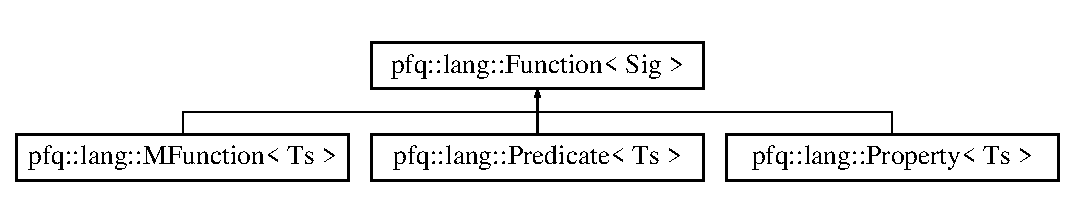
\includegraphics[height=2.000000cm]{structpfq_1_1lang_1_1Function}
\end{center}
\end{figure}
\subsection*{Public Types}
\begin{DoxyCompactItemize}
\item 
using \hyperlink{structpfq_1_1lang_1_1Function_ac7124e473c4804e25b24e9e15fe7b392}{type} = \hyperlink{structpfq_1_1lang_1_1Function}{Function}$<$ Sig $>$
\end{DoxyCompactItemize}


\subsection{Member Typedef Documentation}
\hypertarget{structpfq_1_1lang_1_1Function_ac7124e473c4804e25b24e9e15fe7b392}{\index{pfq\+::lang\+::\+Function@{pfq\+::lang\+::\+Function}!type@{type}}
\index{type@{type}!pfq\+::lang\+::\+Function@{pfq\+::lang\+::\+Function}}
\subsubsection[{type}]{\setlength{\rightskip}{0pt plus 5cm}template$<$typename Sig $>$ using {\bf pfq\+::lang\+::\+Function}$<$ Sig $>$\+::{\bf type} =  {\bf Function}$<$Sig$>$}}\label{structpfq_1_1lang_1_1Function_ac7124e473c4804e25b24e9e15fe7b392}


The documentation for this struct was generated from the following file\+:\begin{DoxyCompactItemize}
\item 
C++/pfq/lang/\hyperlink{lang_8hpp}{lang.\+hpp}\end{DoxyCompactItemize}

\hypertarget{structpfq_1_1lang_1_1FunctionDescr}{\section{pfq\+:\+:lang\+:\+:Function\+Descr Struct Reference}
\label{structpfq_1_1lang_1_1FunctionDescr}\index{pfq\+::lang\+::\+Function\+Descr@{pfq\+::lang\+::\+Function\+Descr}}
}


{\ttfamily \#include $<$lang.\+hpp$>$}

\subsection*{Public Attributes}
\begin{DoxyCompactItemize}
\item 
std\+::string \hyperlink{structpfq_1_1lang_1_1FunctionDescr_a21f51c65f55dddd54de1171d8914c030}{symbol}
\item 
std\+::array$<$ \hyperlink{structpfq_1_1lang_1_1Argument}{Argument}, 4 $>$ \hyperlink{structpfq_1_1lang_1_1FunctionDescr_a2be2814d79d9836cd8e4adbc4dc4e1ca}{arg}
\item 
std\+::size\+\_\+t \hyperlink{structpfq_1_1lang_1_1FunctionDescr_aed683dff23bcead8e4a16ac21ef8ae68}{next}
\end{DoxyCompactItemize}


\subsection{Member Data Documentation}
\hypertarget{structpfq_1_1lang_1_1FunctionDescr_a2be2814d79d9836cd8e4adbc4dc4e1ca}{\index{pfq\+::lang\+::\+Function\+Descr@{pfq\+::lang\+::\+Function\+Descr}!arg@{arg}}
\index{arg@{arg}!pfq\+::lang\+::\+Function\+Descr@{pfq\+::lang\+::\+Function\+Descr}}
\subsubsection[{arg}]{\setlength{\rightskip}{0pt plus 5cm}std\+::array$<${\bf Argument}, 4$>$ pfq\+::lang\+::\+Function\+Descr\+::arg}}\label{structpfq_1_1lang_1_1FunctionDescr_a2be2814d79d9836cd8e4adbc4dc4e1ca}
\hypertarget{structpfq_1_1lang_1_1FunctionDescr_aed683dff23bcead8e4a16ac21ef8ae68}{\index{pfq\+::lang\+::\+Function\+Descr@{pfq\+::lang\+::\+Function\+Descr}!next@{next}}
\index{next@{next}!pfq\+::lang\+::\+Function\+Descr@{pfq\+::lang\+::\+Function\+Descr}}
\subsubsection[{next}]{\setlength{\rightskip}{0pt plus 5cm}std\+::size\+\_\+t pfq\+::lang\+::\+Function\+Descr\+::next}}\label{structpfq_1_1lang_1_1FunctionDescr_aed683dff23bcead8e4a16ac21ef8ae68}
\hypertarget{structpfq_1_1lang_1_1FunctionDescr_a21f51c65f55dddd54de1171d8914c030}{\index{pfq\+::lang\+::\+Function\+Descr@{pfq\+::lang\+::\+Function\+Descr}!symbol@{symbol}}
\index{symbol@{symbol}!pfq\+::lang\+::\+Function\+Descr@{pfq\+::lang\+::\+Function\+Descr}}
\subsubsection[{symbol}]{\setlength{\rightskip}{0pt plus 5cm}std\+::string pfq\+::lang\+::\+Function\+Descr\+::symbol}}\label{structpfq_1_1lang_1_1FunctionDescr_a21f51c65f55dddd54de1171d8914c030}


The documentation for this struct was generated from the following file\+:\begin{DoxyCompactItemize}
\item 
C++/pfq/lang/\hyperlink{lang_8hpp}{lang.\+hpp}\end{DoxyCompactItemize}

\hypertarget{structpfq_1_1lang_1_1funptr__t}{}\section{pfq\+:\+:lang\+:\+:funptr\+\_\+t Struct Reference}
\label{structpfq_1_1lang_1_1funptr__t}\index{pfq\+::lang\+::funptr\+\_\+t@{pfq\+::lang\+::funptr\+\_\+t}}


{\ttfamily \#include $<$lang.\+hpp$>$}



The documentation for this struct was generated from the following file\+:\begin{DoxyCompactItemize}
\item 
C++/pfq/lang/\hyperlink{lang_8hpp}{lang.\+hpp}\end{DoxyCompactItemize}

\hypertarget{structpfq_1_1lang_1_1ipv4__t}{}\section{pfq\+:\+:lang\+:\+:ipv4\+\_\+t Struct Reference}
\label{structpfq_1_1lang_1_1ipv4__t}\index{pfq\+::lang\+::ipv4\+\_\+t@{pfq\+::lang\+::ipv4\+\_\+t}}


{\ttfamily \#include $<$lang.\+hpp$>$}

\subsection*{Public Member Functions}
\begin{DoxyCompactItemize}
\item 
\hyperlink{structpfq_1_1lang_1_1ipv4__t_a3237166f3fab90a77846d9656b0482c8}{ipv4\+\_\+t} ()=default
\item 
\hyperlink{structpfq_1_1lang_1_1ipv4__t_a86fa55f6ef31157415d65d43ce228fae}{ipv4\+\_\+t} (const char $\ast$addr)
\end{DoxyCompactItemize}
\subsection*{Public Attributes}
\begin{DoxyCompactItemize}
\item 
uint32\+\_\+t \hyperlink{structpfq_1_1lang_1_1ipv4__t_a5080d5f65781ad95e605d066f1693502}{value}
\end{DoxyCompactItemize}


\subsection{Constructor \& Destructor Documentation}
\index{pfq\+::lang\+::ipv4\+\_\+t@{pfq\+::lang\+::ipv4\+\_\+t}!ipv4\+\_\+t@{ipv4\+\_\+t}}
\index{ipv4\+\_\+t@{ipv4\+\_\+t}!pfq\+::lang\+::ipv4\+\_\+t@{pfq\+::lang\+::ipv4\+\_\+t}}
\subsubsection[{\texorpdfstring{ipv4\+\_\+t()=default}{ipv4_t()=default}}]{\setlength{\rightskip}{0pt plus 5cm}pfq\+::lang\+::ipv4\+\_\+t\+::ipv4\+\_\+t (
\begin{DoxyParamCaption}
{}
\end{DoxyParamCaption}
)\hspace{0.3cm}{\ttfamily [default]}}\hypertarget{structpfq_1_1lang_1_1ipv4__t_a3237166f3fab90a77846d9656b0482c8}{}\label{structpfq_1_1lang_1_1ipv4__t_a3237166f3fab90a77846d9656b0482c8}
\index{pfq\+::lang\+::ipv4\+\_\+t@{pfq\+::lang\+::ipv4\+\_\+t}!ipv4\+\_\+t@{ipv4\+\_\+t}}
\index{ipv4\+\_\+t@{ipv4\+\_\+t}!pfq\+::lang\+::ipv4\+\_\+t@{pfq\+::lang\+::ipv4\+\_\+t}}
\subsubsection[{\texorpdfstring{ipv4\+\_\+t(const char $\ast$addr)}{ipv4_t(const char *addr)}}]{\setlength{\rightskip}{0pt plus 5cm}pfq\+::lang\+::ipv4\+\_\+t\+::ipv4\+\_\+t (
\begin{DoxyParamCaption}
\item[{const char $\ast$}]{addr}
\end{DoxyParamCaption}
)\hspace{0.3cm}{\ttfamily [inline]}}\hypertarget{structpfq_1_1lang_1_1ipv4__t_a86fa55f6ef31157415d65d43ce228fae}{}\label{structpfq_1_1lang_1_1ipv4__t_a86fa55f6ef31157415d65d43ce228fae}


\subsection{Member Data Documentation}
\index{pfq\+::lang\+::ipv4\+\_\+t@{pfq\+::lang\+::ipv4\+\_\+t}!value@{value}}
\index{value@{value}!pfq\+::lang\+::ipv4\+\_\+t@{pfq\+::lang\+::ipv4\+\_\+t}}
\subsubsection[{\texorpdfstring{value}{value}}]{\setlength{\rightskip}{0pt plus 5cm}uint32\+\_\+t pfq\+::lang\+::ipv4\+\_\+t\+::value}\hypertarget{structpfq_1_1lang_1_1ipv4__t_a5080d5f65781ad95e605d066f1693502}{}\label{structpfq_1_1lang_1_1ipv4__t_a5080d5f65781ad95e605d066f1693502}


The documentation for this struct was generated from the following file\+:\begin{DoxyCompactItemize}
\item 
C++/pfq/lang/\hyperlink{lang_8hpp}{lang.\+hpp}\end{DoxyCompactItemize}

\hypertarget{structpfq_1_1lang_1_1is__monadic__function}{}\section{pfq\+:\+:lang\+:\+:is\+\_\+monadic\+\_\+function$<$ Tp $>$ Struct Template Reference}
\label{structpfq_1_1lang_1_1is__monadic__function}\index{pfq\+::lang\+::is\+\_\+monadic\+\_\+function$<$ Tp $>$@{pfq\+::lang\+::is\+\_\+monadic\+\_\+function$<$ Tp $>$}}


{\ttfamily \#include $<$lang.\+hpp$>$}

Inheritance diagram for pfq\+:\+:lang\+:\+:is\+\_\+monadic\+\_\+function$<$ Tp $>$\+:\begin{figure}[H]
\begin{center}
\leavevmode
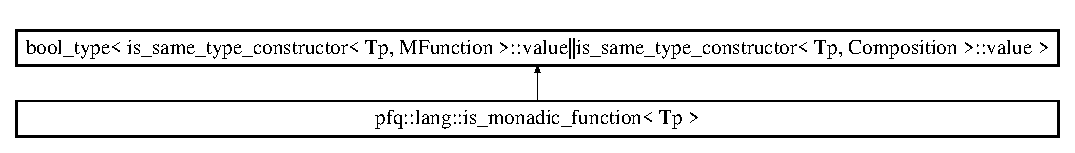
\includegraphics[height=1.637427cm]{structpfq_1_1lang_1_1is__monadic__function}
\end{center}
\end{figure}


The documentation for this struct was generated from the following file\+:\begin{DoxyCompactItemize}
\item 
C++/pfq/lang/\hyperlink{lang_8hpp}{lang.\+hpp}\end{DoxyCompactItemize}

\hypertarget{structpfq_1_1lang_1_1is__predicate}{\section{pfq\+:\+:lang\+:\+:is\+\_\+predicate$<$ Tp $>$ Struct Template Reference}
\label{structpfq_1_1lang_1_1is__predicate}\index{pfq\+::lang\+::is\+\_\+predicate$<$ Tp $>$@{pfq\+::lang\+::is\+\_\+predicate$<$ Tp $>$}}
}


{\ttfamily \#include $<$lang.\+hpp$>$}

Inheritance diagram for pfq\+:\+:lang\+:\+:is\+\_\+predicate$<$ Tp $>$\+:\begin{figure}[H]
\begin{center}
\leavevmode
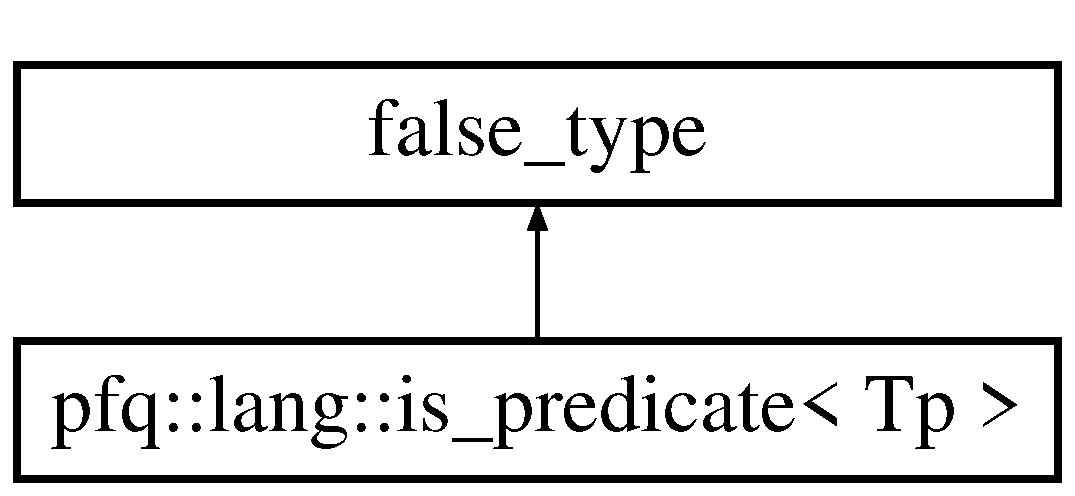
\includegraphics[height=0.645905cm]{structpfq_1_1lang_1_1is__predicate}
\end{center}
\end{figure}


The documentation for this struct was generated from the following file\+:\begin{DoxyCompactItemize}
\item 
C++/pfq-\/lang/\hyperlink{lang_8hpp}{lang.\+hpp}\end{DoxyCompactItemize}

\hypertarget{structpfq_1_1lang_1_1is__predicate_3_01Predicate_3_01Ts_8_8_8_4_01_4}{\section{pfq\+:\+:lang\+:\+:is\+\_\+predicate$<$ Predicate$<$ Ts...$>$ $>$ Struct Template Reference}
\label{structpfq_1_1lang_1_1is__predicate_3_01Predicate_3_01Ts_8_8_8_4_01_4}\index{pfq\+::lang\+::is\+\_\+predicate$<$ Predicate$<$ Ts...$>$ $>$@{pfq\+::lang\+::is\+\_\+predicate$<$ Predicate$<$ Ts...$>$ $>$}}
}


{\ttfamily \#include $<$lang.\+hpp$>$}

Inheritance diagram for pfq\+:\+:lang\+:\+:is\+\_\+predicate$<$ Predicate$<$ Ts...$>$ $>$\+:\begin{figure}[H]
\begin{center}
\leavevmode
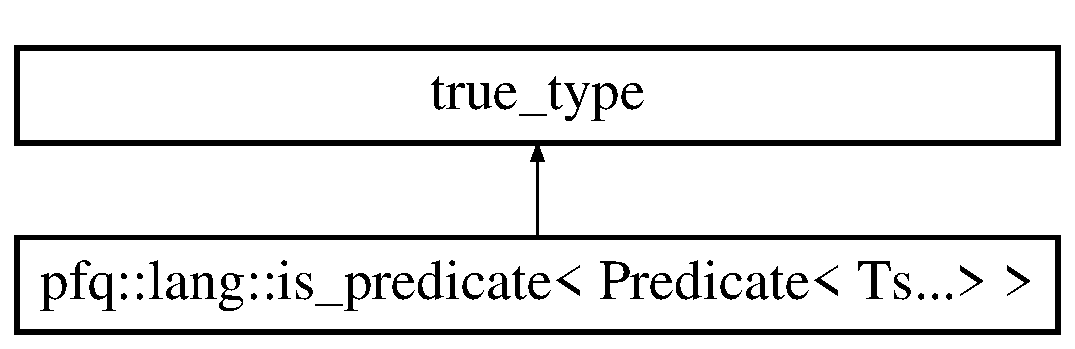
\includegraphics[height=2.000000cm]{structpfq_1_1lang_1_1is__predicate_3_01Predicate_3_01Ts_8_8_8_4_01_4}
\end{center}
\end{figure}


The documentation for this struct was generated from the following file\+:\begin{DoxyCompactItemize}
\item 
C++/pfq/lang/\hyperlink{lang_8hpp}{lang.\+hpp}\end{DoxyCompactItemize}

\hypertarget{structpfq_1_1lang_1_1is__property}{\section{pfq\+:\+:lang\+:\+:is\+\_\+property$<$ Tp $>$ Struct Template Reference}
\label{structpfq_1_1lang_1_1is__property}\index{pfq\+::lang\+::is\+\_\+property$<$ Tp $>$@{pfq\+::lang\+::is\+\_\+property$<$ Tp $>$}}
}


{\ttfamily \#include $<$lang.\+hpp$>$}

Inheritance diagram for pfq\+:\+:lang\+:\+:is\+\_\+property$<$ Tp $>$\+:\begin{figure}[H]
\begin{center}
\leavevmode
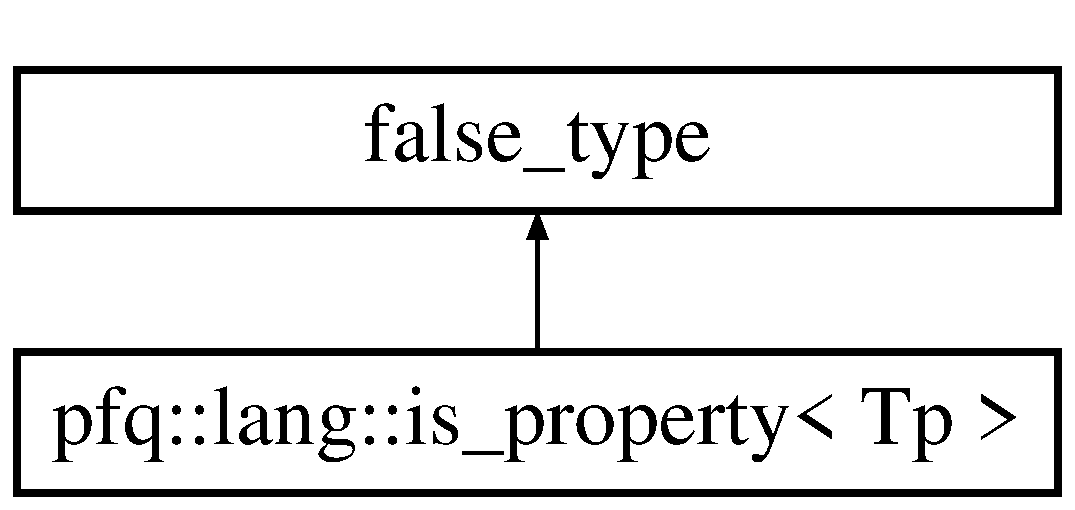
\includegraphics[height=2.000000cm]{structpfq_1_1lang_1_1is__property}
\end{center}
\end{figure}


The documentation for this struct was generated from the following file\+:\begin{DoxyCompactItemize}
\item 
C++/pfq/lang/\hyperlink{lang_8hpp}{lang.\+hpp}\end{DoxyCompactItemize}

\hypertarget{structpfq_1_1lang_1_1is__property_3_01Property_3_01Ts_8_8_8_4_01_4}{\section{pfq\+:\+:lang\+:\+:is\+\_\+property$<$ Property$<$ Ts...$>$ $>$ Struct Template Reference}
\label{structpfq_1_1lang_1_1is__property_3_01Property_3_01Ts_8_8_8_4_01_4}\index{pfq\+::lang\+::is\+\_\+property$<$ Property$<$ Ts...$>$ $>$@{pfq\+::lang\+::is\+\_\+property$<$ Property$<$ Ts...$>$ $>$}}
}


{\ttfamily \#include $<$lang.\+hpp$>$}

Inheritance diagram for pfq\+:\+:lang\+:\+:is\+\_\+property$<$ Property$<$ Ts...$>$ $>$\+:\begin{figure}[H]
\begin{center}
\leavevmode
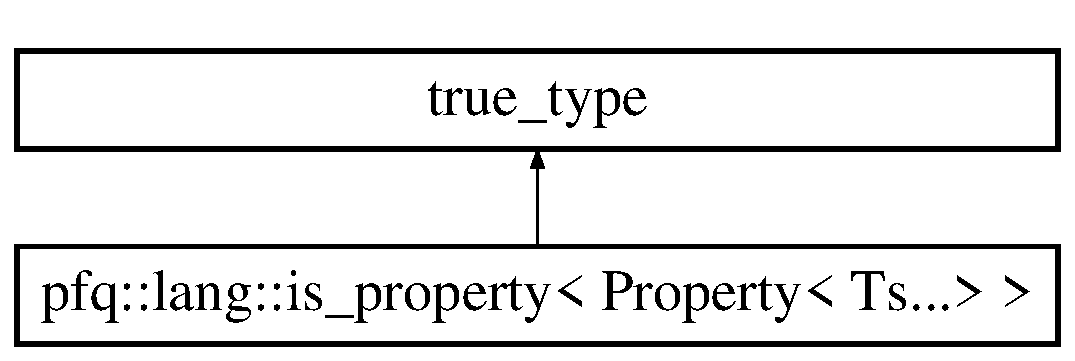
\includegraphics[height=2.000000cm]{structpfq_1_1lang_1_1is__property_3_01Property_3_01Ts_8_8_8_4_01_4}
\end{center}
\end{figure}


The documentation for this struct was generated from the following file\+:\begin{DoxyCompactItemize}
\item 
C++/pfq/lang/\hyperlink{lang_8hpp}{lang.\+hpp}\end{DoxyCompactItemize}

\hypertarget{structpfq_1_1lang_1_1kleisly}{\section{pfq\+:\+:lang\+:\+:kleisly$<$ F, G $>$ Struct Template Reference}
\label{structpfq_1_1lang_1_1kleisly}\index{pfq\+::lang\+::kleisly$<$ F, G $>$@{pfq\+::lang\+::kleisly$<$ F, G $>$}}
}


{\ttfamily \#include $<$lang.\+hpp$>$}



The documentation for this struct was generated from the following file\+:\begin{DoxyCompactItemize}
\item 
C++/pfq-\/lang/\hyperlink{lang_8hpp}{lang.\+hpp}\end{DoxyCompactItemize}

\hypertarget{structpfq_1_1lang_1_1kleisly_3_01Function_3_01M_3_01B_01_4_07A_08_01_4_00_01Composition_3_01F_00_01G_01_4_01_4}{\section{pfq\+:\+:lang\+:\+:kleisly$<$ Function$<$ M$<$ B $>$(A) $>$, Composition$<$ F, G $>$ $>$ Struct Template Reference}
\label{structpfq_1_1lang_1_1kleisly_3_01Function_3_01M_3_01B_01_4_07A_08_01_4_00_01Composition_3_01F_00_01G_01_4_01_4}\index{pfq\+::lang\+::kleisly$<$ Function$<$ M$<$ B $>$(\+A) $>$, Composition$<$ F, G $>$ $>$@{pfq\+::lang\+::kleisly$<$ Function$<$ M$<$ B $>$(\+A) $>$, Composition$<$ F, G $>$ $>$}}
}


{\ttfamily \#include $<$lang.\+hpp$>$}

\subsection*{Public Types}
\begin{DoxyCompactItemize}
\item 
using \hyperlink{structpfq_1_1lang_1_1kleisly_3_01Function_3_01M_3_01B_01_4_07A_08_01_4_00_01Composition_3_01F_00_01G_01_4_01_4_aa5c026817ce615e5e51ed76159b2e759}{type} = typename \hyperlink{structpfq_1_1lang_1_1kleisly}{kleisly}$<$ \hyperlink{structpfq_1_1lang_1_1Function}{Function}$<$ M$<$ B $>$(A)$>$, typename \hyperlink{structpfq_1_1lang_1_1kleisly}{kleisly}$<$ F, G $>$\+::\hyperlink{structpfq_1_1lang_1_1kleisly_3_01Function_3_01M_3_01B_01_4_07A_08_01_4_00_01Composition_3_01F_00_01G_01_4_01_4_aa5c026817ce615e5e51ed76159b2e759}{type} $>$\+::\hyperlink{structpfq_1_1lang_1_1kleisly_3_01Function_3_01M_3_01B_01_4_07A_08_01_4_00_01Composition_3_01F_00_01G_01_4_01_4_aa5c026817ce615e5e51ed76159b2e759}{type}
\end{DoxyCompactItemize}


\subsection{Member Typedef Documentation}
\hypertarget{structpfq_1_1lang_1_1kleisly_3_01Function_3_01M_3_01B_01_4_07A_08_01_4_00_01Composition_3_01F_00_01G_01_4_01_4_aa5c026817ce615e5e51ed76159b2e759}{\index{pfq\+::lang\+::kleisly$<$ Function$<$ M$<$ B $>$(\+A) $>$, Composition$<$ F, G $>$ $>$@{pfq\+::lang\+::kleisly$<$ Function$<$ M$<$ B $>$(\+A) $>$, Composition$<$ F, G $>$ $>$}!type@{type}}
\index{type@{type}!pfq\+::lang\+::kleisly$<$ Function$<$ M$<$ B $>$(\+A) $>$, Composition$<$ F, G $>$ $>$@{pfq\+::lang\+::kleisly$<$ Function$<$ M$<$ B $>$(\+A) $>$, Composition$<$ F, G $>$ $>$}}
\subsubsection[{type}]{\setlength{\rightskip}{0pt plus 5cm}template$<$template$<$ typename $>$ class M, typename A , typename B , typename F , typename G $>$ using {\bf pfq\+::lang\+::kleisly}$<$ {\bf Function}$<$ M$<$ B $>$(A) $>$, {\bf Composition}$<$ F, G $>$ $>$\+::{\bf type} =  typename {\bf kleisly}$<$ {\bf Function}$<$M$<$B$>$(A)$>$, typename {\bf kleisly}$<$F,G$>$\+::{\bf type}$>$\+::{\bf type}}}\label{structpfq_1_1lang_1_1kleisly_3_01Function_3_01M_3_01B_01_4_07A_08_01_4_00_01Composition_3_01F_00_01G_01_4_01_4_aa5c026817ce615e5e51ed76159b2e759}


The documentation for this struct was generated from the following file\+:\begin{DoxyCompactItemize}
\item 
C++/pfq-\/lang/\hyperlink{lang_8hpp}{lang.\+hpp}\end{DoxyCompactItemize}

\hypertarget{structpfq_1_1lang_1_1kleisly_3_01Function_3_01M_3_01B_01_4_07A_08_01_4_00_01Function_3_01M_3_01C_01_4_07B_08_4_01_4}{\section{pfq\+:\+:lang\+:\+:kleisly$<$ Function$<$ M$<$ B $>$(A) $>$, Function$<$ M$<$ C $>$(B)$>$ $>$ Struct Template Reference}
\label{structpfq_1_1lang_1_1kleisly_3_01Function_3_01M_3_01B_01_4_07A_08_01_4_00_01Function_3_01M_3_01C_01_4_07B_08_4_01_4}\index{pfq\+::lang\+::kleisly$<$ Function$<$ M$<$ B $>$(\+A) $>$, Function$<$ M$<$ C $>$(\+B)$>$ $>$@{pfq\+::lang\+::kleisly$<$ Function$<$ M$<$ B $>$(\+A) $>$, Function$<$ M$<$ C $>$(\+B)$>$ $>$}}
}


{\ttfamily \#include $<$lang.\+hpp$>$}

\subsection*{Public Types}
\begin{DoxyCompactItemize}
\item 
using \hyperlink{structpfq_1_1lang_1_1kleisly_3_01Function_3_01M_3_01B_01_4_07A_08_01_4_00_01Function_3_01M_3_01C_01_4_07B_08_4_01_4_add8114ae2219624ca829d1409d6695bc}{type} = \hyperlink{structpfq_1_1lang_1_1Function}{Function}$<$ M$<$ C $>$(A) $>$
\end{DoxyCompactItemize}


\subsection{Member Typedef Documentation}
\hypertarget{structpfq_1_1lang_1_1kleisly_3_01Function_3_01M_3_01B_01_4_07A_08_01_4_00_01Function_3_01M_3_01C_01_4_07B_08_4_01_4_add8114ae2219624ca829d1409d6695bc}{\index{pfq\+::lang\+::kleisly$<$ Function$<$ M$<$ B $>$(\+A) $>$, Function$<$ M$<$ C $>$(\+B)$>$ $>$@{pfq\+::lang\+::kleisly$<$ Function$<$ M$<$ B $>$(\+A) $>$, Function$<$ M$<$ C $>$(\+B)$>$ $>$}!type@{type}}
\index{type@{type}!pfq\+::lang\+::kleisly$<$ Function$<$ M$<$ B $>$(\+A) $>$, Function$<$ M$<$ C $>$(\+B)$>$ $>$@{pfq\+::lang\+::kleisly$<$ Function$<$ M$<$ B $>$(\+A) $>$, Function$<$ M$<$ C $>$(\+B)$>$ $>$}}
\subsubsection[{type}]{\setlength{\rightskip}{0pt plus 5cm}template$<$template$<$ typename $>$ class M, typename A , typename B , typename C $>$ using {\bf pfq\+::lang\+::kleisly}$<$ {\bf Function}$<$ M$<$ B $>$(A) $>$, {\bf Function}$<$ M$<$ C $>$(B)$>$ $>$\+::{\bf type} =  {\bf Function} $<$ M$<$C$>$(A) $>$}}\label{structpfq_1_1lang_1_1kleisly_3_01Function_3_01M_3_01B_01_4_07A_08_01_4_00_01Function_3_01M_3_01C_01_4_07B_08_4_01_4_add8114ae2219624ca829d1409d6695bc}


The documentation for this struct was generated from the following file\+:\begin{DoxyCompactItemize}
\item 
C++/pfq-\/lang/\hyperlink{lang_8hpp}{lang.\+hpp}\end{DoxyCompactItemize}

\hypertarget{structpfq_1_1lang_1_1MFunction}{\section{pfq\+:\+:lang\+:\+:M\+Function$<$ Ts $>$ Struct Template Reference}
\label{structpfq_1_1lang_1_1MFunction}\index{pfq\+::lang\+::\+M\+Function$<$ Ts $>$@{pfq\+::lang\+::\+M\+Function$<$ Ts $>$}}
}


{\ttfamily \#include $<$lang.\+hpp$>$}

Inheritance diagram for pfq\+:\+:lang\+:\+:M\+Function$<$ Ts $>$\+:\begin{figure}[H]
\begin{center}
\leavevmode
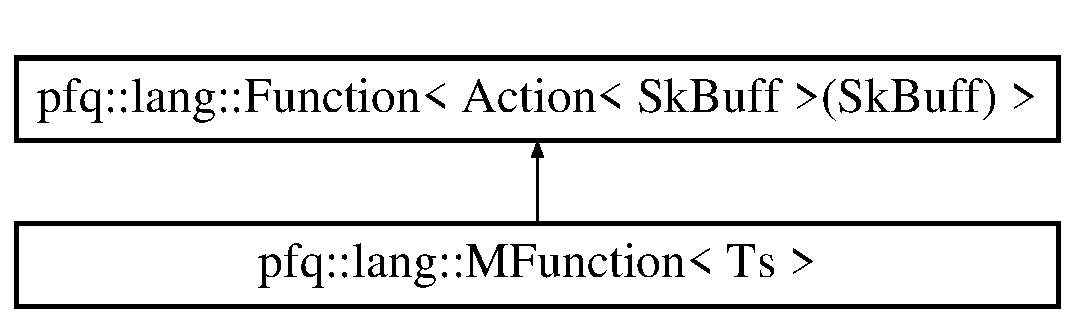
\includegraphics[height=2.000000cm]{structpfq_1_1lang_1_1MFunction}
\end{center}
\end{figure}
\subsection*{Public Member Functions}
\begin{DoxyCompactItemize}
\item 
{\footnotesize template$<$typename... Tp$>$ }\\\hyperlink{structpfq_1_1lang_1_1MFunction_a11626b481dd2a377eba5b472bffaec19}{M\+Function} (std\+::string symbol, Tp \&\&...args)
\end{DoxyCompactItemize}
\subsection*{Public Attributes}
\begin{DoxyCompactItemize}
\item 
std\+::string \hyperlink{structpfq_1_1lang_1_1MFunction_ad71e16a351d465079c8c4cc014157b2b}{symbol\+\_\+}
\item 
std\+::tuple$<$ Ts...$>$ \hyperlink{structpfq_1_1lang_1_1MFunction_a3259c7f79ac8c60bba3462bc01b859f7}{args\+\_\+}
\end{DoxyCompactItemize}
\subsection*{Additional Inherited Members}


\subsection{Constructor \& Destructor Documentation}
\hypertarget{structpfq_1_1lang_1_1MFunction_a11626b481dd2a377eba5b472bffaec19}{\index{pfq\+::lang\+::\+M\+Function@{pfq\+::lang\+::\+M\+Function}!M\+Function@{M\+Function}}
\index{M\+Function@{M\+Function}!pfq\+::lang\+::\+M\+Function@{pfq\+::lang\+::\+M\+Function}}
\subsubsection[{M\+Function}]{\setlength{\rightskip}{0pt plus 5cm}template$<$typename... Ts$>$ template$<$typename... Tp$>$ {\bf pfq\+::lang\+::\+M\+Function}$<$ Ts $>$\+::{\bf M\+Function} (
\begin{DoxyParamCaption}
\item[{std\+::string}]{symbol, }
\item[{Tp \&\&...}]{args}
\end{DoxyParamCaption}
)\hspace{0.3cm}{\ttfamily [inline]}}}\label{structpfq_1_1lang_1_1MFunction_a11626b481dd2a377eba5b472bffaec19}


\subsection{Member Data Documentation}
\hypertarget{structpfq_1_1lang_1_1MFunction_a3259c7f79ac8c60bba3462bc01b859f7}{\index{pfq\+::lang\+::\+M\+Function@{pfq\+::lang\+::\+M\+Function}!args\+\_\+@{args\+\_\+}}
\index{args\+\_\+@{args\+\_\+}!pfq\+::lang\+::\+M\+Function@{pfq\+::lang\+::\+M\+Function}}
\subsubsection[{args\+\_\+}]{\setlength{\rightskip}{0pt plus 5cm}template$<$typename... Ts$>$ std\+::tuple$<$Ts...$>$ {\bf pfq\+::lang\+::\+M\+Function}$<$ Ts $>$\+::args\+\_\+}}\label{structpfq_1_1lang_1_1MFunction_a3259c7f79ac8c60bba3462bc01b859f7}
\hypertarget{structpfq_1_1lang_1_1MFunction_ad71e16a351d465079c8c4cc014157b2b}{\index{pfq\+::lang\+::\+M\+Function@{pfq\+::lang\+::\+M\+Function}!symbol\+\_\+@{symbol\+\_\+}}
\index{symbol\+\_\+@{symbol\+\_\+}!pfq\+::lang\+::\+M\+Function@{pfq\+::lang\+::\+M\+Function}}
\subsubsection[{symbol\+\_\+}]{\setlength{\rightskip}{0pt plus 5cm}template$<$typename... Ts$>$ std\+::string {\bf pfq\+::lang\+::\+M\+Function}$<$ Ts $>$\+::symbol\+\_\+}}\label{structpfq_1_1lang_1_1MFunction_ad71e16a351d465079c8c4cc014157b2b}


The documentation for this struct was generated from the following file\+:\begin{DoxyCompactItemize}
\item 
C++/pfq/lang/\hyperlink{lang_8hpp}{lang.\+hpp}\end{DoxyCompactItemize}

\hypertarget{structpfq_1_1lang_1_1Predicate}{}\section{pfq\+:\+:lang\+:\+:Predicate$<$ Ts $>$ Struct Template Reference}
\label{structpfq_1_1lang_1_1Predicate}\index{pfq\+::lang\+::\+Predicate$<$ Ts $>$@{pfq\+::lang\+::\+Predicate$<$ Ts $>$}}


{\ttfamily \#include $<$lang.\+hpp$>$}

Inheritance diagram for pfq\+:\+:lang\+:\+:Predicate$<$ Ts $>$\+:\begin{figure}[H]
\begin{center}
\leavevmode
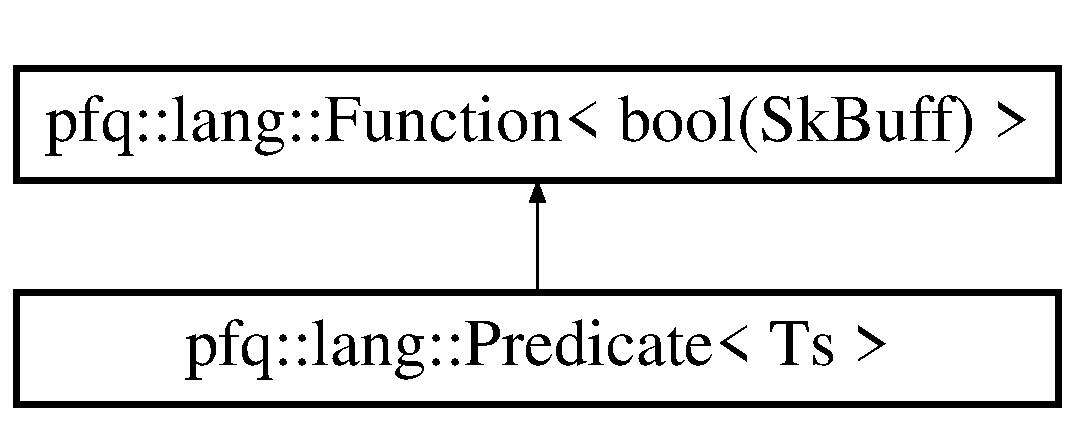
\includegraphics[height=2.000000cm]{structpfq_1_1lang_1_1Predicate}
\end{center}
\end{figure}
\subsection*{Public Member Functions}
\begin{DoxyCompactItemize}
\item 
{\footnotesize template$<$typename... Tp$>$ }\\\hyperlink{structpfq_1_1lang_1_1Predicate_ad604e102c7599051e801d790cca70591}{Predicate} (std\+::string symbol, Tp \&\&...args)
\end{DoxyCompactItemize}
\subsection*{Public Attributes}
\begin{DoxyCompactItemize}
\item 
std\+::string \hyperlink{structpfq_1_1lang_1_1Predicate_a5f3219d34d216f1af9f6b1cafb93cc62}{symbol\+\_\+}
\item 
std\+::tuple$<$ Ts... $>$ \hyperlink{structpfq_1_1lang_1_1Predicate_aee302feb9cdf55566e50249e6dcd50af}{args\+\_\+}
\end{DoxyCompactItemize}
\subsection*{Additional Inherited Members}


\subsection{Constructor \& Destructor Documentation}
\index{pfq\+::lang\+::\+Predicate@{pfq\+::lang\+::\+Predicate}!Predicate@{Predicate}}
\index{Predicate@{Predicate}!pfq\+::lang\+::\+Predicate@{pfq\+::lang\+::\+Predicate}}
\subsubsection[{\texorpdfstring{Predicate(std\+::string symbol, Tp \&\&...\+args)}{Predicate(std::string symbol, Tp &&...args)}}]{\setlength{\rightskip}{0pt plus 5cm}template$<$typename... Ts$>$ template$<$typename... Tp$>$ {\bf pfq\+::lang\+::\+Predicate}$<$ Ts $>$\+::{\bf Predicate} (
\begin{DoxyParamCaption}
\item[{std\+::string}]{symbol, }
\item[{Tp \&\&...}]{args}
\end{DoxyParamCaption}
)\hspace{0.3cm}{\ttfamily [inline]}}\hypertarget{structpfq_1_1lang_1_1Predicate_ad604e102c7599051e801d790cca70591}{}\label{structpfq_1_1lang_1_1Predicate_ad604e102c7599051e801d790cca70591}


\subsection{Member Data Documentation}
\index{pfq\+::lang\+::\+Predicate@{pfq\+::lang\+::\+Predicate}!args\+\_\+@{args\+\_\+}}
\index{args\+\_\+@{args\+\_\+}!pfq\+::lang\+::\+Predicate@{pfq\+::lang\+::\+Predicate}}
\subsubsection[{\texorpdfstring{args\+\_\+}{args_}}]{\setlength{\rightskip}{0pt plus 5cm}template$<$typename... Ts$>$ std\+::tuple$<$Ts...$>$ {\bf pfq\+::lang\+::\+Predicate}$<$ Ts $>$\+::args\+\_\+}\hypertarget{structpfq_1_1lang_1_1Predicate_aee302feb9cdf55566e50249e6dcd50af}{}\label{structpfq_1_1lang_1_1Predicate_aee302feb9cdf55566e50249e6dcd50af}
\index{pfq\+::lang\+::\+Predicate@{pfq\+::lang\+::\+Predicate}!symbol\+\_\+@{symbol\+\_\+}}
\index{symbol\+\_\+@{symbol\+\_\+}!pfq\+::lang\+::\+Predicate@{pfq\+::lang\+::\+Predicate}}
\subsubsection[{\texorpdfstring{symbol\+\_\+}{symbol_}}]{\setlength{\rightskip}{0pt plus 5cm}template$<$typename... Ts$>$ std\+::string {\bf pfq\+::lang\+::\+Predicate}$<$ Ts $>$\+::symbol\+\_\+}\hypertarget{structpfq_1_1lang_1_1Predicate_a5f3219d34d216f1af9f6b1cafb93cc62}{}\label{structpfq_1_1lang_1_1Predicate_a5f3219d34d216f1af9f6b1cafb93cc62}


The documentation for this struct was generated from the following file\+:\begin{DoxyCompactItemize}
\item 
C++/pfq/lang/\hyperlink{lang_8hpp}{lang.\+hpp}\end{DoxyCompactItemize}

\hypertarget{structpfq_1_1lang_1_1Property}{\section{pfq\+:\+:lang\+:\+:Property$<$ Ts $>$ Struct Template Reference}
\label{structpfq_1_1lang_1_1Property}\index{pfq\+::lang\+::\+Property$<$ Ts $>$@{pfq\+::lang\+::\+Property$<$ Ts $>$}}
}


{\ttfamily \#include $<$lang.\+hpp$>$}

Inheritance diagram for pfq\+:\+:lang\+:\+:Property$<$ Ts $>$\+:\begin{figure}[H]
\begin{center}
\leavevmode
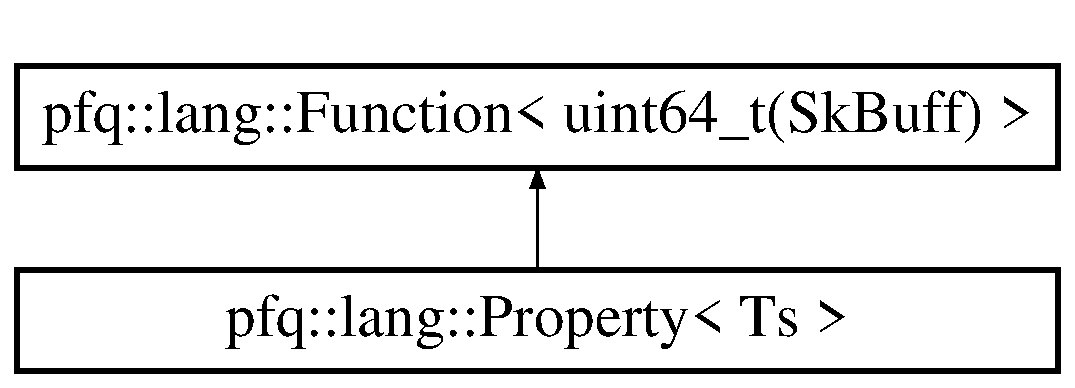
\includegraphics[height=2.000000cm]{structpfq_1_1lang_1_1Property}
\end{center}
\end{figure}
\subsection*{Public Member Functions}
\begin{DoxyCompactItemize}
\item 
{\footnotesize template$<$typename... Tp$>$ }\\\hyperlink{structpfq_1_1lang_1_1Property_a65d215ea79feeaf43feaa02f3c8a31a4}{Property} (std\+::string symbol, Tp \&\&...args)
\end{DoxyCompactItemize}
\subsection*{Public Attributes}
\begin{DoxyCompactItemize}
\item 
std\+::string \hyperlink{structpfq_1_1lang_1_1Property_a27cdbc97fd6ffc8b92ff75599c7dce72}{symbol\+\_\+}
\item 
std\+::tuple$<$ Ts...$>$ \hyperlink{structpfq_1_1lang_1_1Property_a01e0bf793226860cbafe4bea5075d507}{args\+\_\+}
\end{DoxyCompactItemize}
\subsection*{Additional Inherited Members}


\subsection{Constructor \& Destructor Documentation}
\hypertarget{structpfq_1_1lang_1_1Property_a65d215ea79feeaf43feaa02f3c8a31a4}{\index{pfq\+::lang\+::\+Property@{pfq\+::lang\+::\+Property}!Property@{Property}}
\index{Property@{Property}!pfq\+::lang\+::\+Property@{pfq\+::lang\+::\+Property}}
\subsubsection[{Property}]{\setlength{\rightskip}{0pt plus 5cm}template$<$typename... Ts$>$ template$<$typename... Tp$>$ {\bf pfq\+::lang\+::\+Property}$<$ Ts $>$\+::{\bf Property} (
\begin{DoxyParamCaption}
\item[{std\+::string}]{symbol, }
\item[{Tp \&\&...}]{args}
\end{DoxyParamCaption}
)\hspace{0.3cm}{\ttfamily [inline]}}}\label{structpfq_1_1lang_1_1Property_a65d215ea79feeaf43feaa02f3c8a31a4}


\subsection{Member Data Documentation}
\hypertarget{structpfq_1_1lang_1_1Property_a01e0bf793226860cbafe4bea5075d507}{\index{pfq\+::lang\+::\+Property@{pfq\+::lang\+::\+Property}!args\+\_\+@{args\+\_\+}}
\index{args\+\_\+@{args\+\_\+}!pfq\+::lang\+::\+Property@{pfq\+::lang\+::\+Property}}
\subsubsection[{args\+\_\+}]{\setlength{\rightskip}{0pt plus 5cm}template$<$typename... Ts$>$ std\+::tuple$<$Ts...$>$ {\bf pfq\+::lang\+::\+Property}$<$ Ts $>$\+::args\+\_\+}}\label{structpfq_1_1lang_1_1Property_a01e0bf793226860cbafe4bea5075d507}
\hypertarget{structpfq_1_1lang_1_1Property_a27cdbc97fd6ffc8b92ff75599c7dce72}{\index{pfq\+::lang\+::\+Property@{pfq\+::lang\+::\+Property}!symbol\+\_\+@{symbol\+\_\+}}
\index{symbol\+\_\+@{symbol\+\_\+}!pfq\+::lang\+::\+Property@{pfq\+::lang\+::\+Property}}
\subsubsection[{symbol\+\_\+}]{\setlength{\rightskip}{0pt plus 5cm}template$<$typename... Ts$>$ std\+::string {\bf pfq\+::lang\+::\+Property}$<$ Ts $>$\+::symbol\+\_\+}}\label{structpfq_1_1lang_1_1Property_a27cdbc97fd6ffc8b92ff75599c7dce72}


The documentation for this struct was generated from the following file\+:\begin{DoxyCompactItemize}
\item 
C++/pfq/lang/\hyperlink{lang_8hpp}{lang.\+hpp}\end{DoxyCompactItemize}

\hypertarget{structpfq_1_1lang_1_1SkBuff}{}\section{pfq\+:\+:lang\+:\+:Sk\+Buff Struct Reference}
\label{structpfq_1_1lang_1_1SkBuff}\index{pfq\+::lang\+::\+Sk\+Buff@{pfq\+::lang\+::\+Sk\+Buff}}


{\ttfamily \#include $<$lang.\+hpp$>$}



The documentation for this struct was generated from the following file\+:\begin{DoxyCompactItemize}
\item 
C++/pfq/lang/\hyperlink{lang_8hpp}{lang.\+hpp}\end{DoxyCompactItemize}

\chapter{File Documentation}
\hypertarget{default_8hpp}{\section{C++/pfq-\/lang/default.hpp File Reference}
\label{default_8hpp}\index{C++/pfq-\/lang/default.\+hpp@{C++/pfq-\/lang/default.\+hpp}}
}
{\ttfamily \#include $<$pfq-\/lang/lang.\+hpp$>$}\\*
{\ttfamily \#include $<$pfq-\/lang/details.\+hpp$>$}\\*
{\ttfamily \#include $<$functional$>$}\\*
{\ttfamily \#include $<$arpa/inet.\+h$>$}\\*
\subsection*{Namespaces}
\begin{DoxyCompactItemize}
\item 
 \hyperlink{namespacepfq__lang}{pfq\+\_\+lang}
\item 
 \hyperlink{namespacepfq__lang_1_1anonymous__namespace_02default_8hpp_03}{pfq\+\_\+lang\+::anonymous\+\_\+namespace\{default.\+hpp\}}
\end{DoxyCompactItemize}
\subsection*{Functions}
\begin{DoxyCompactItemize}
\item 
{\footnotesize template$<$typename P1 , typename P2 $>$ }\\auto \hyperlink{namespacepfq__lang_aa6f7aa80466e4cfd61a341fcf7a2eda4}{pfq\+\_\+lang\+::operator\&} (P1 const \&p1, P2 const \&p2) -\/$>$ decltype(predicate2(combinator(nullptr), p1, p2))
\item 
{\footnotesize template$<$typename P1 , typename P2 $>$ }\\auto \hyperlink{namespacepfq__lang_adeec773d44aae2b2f2957e1498c4ce8f}{pfq\+\_\+lang\+::operator$\vert$} (P1 const \&p1, P2 const \&p2) -\/$>$ decltype(predicate2(combinator(nullptr), p1, p2))
\item 
{\footnotesize template$<$typename P1 , typename P2 $>$ }\\auto \hyperlink{namespacepfq__lang_a29166c6bb957d6edd6892b7081f574df}{pfq\+\_\+lang\+::operator$^\wedge$} (P1 const \&p1, P2 const \&p2) -\/$>$ decltype(predicate2(combinator(nullptr), p1, p2))
\item 
{\footnotesize template$<$typename P $>$ }\\auto \hyperlink{namespacepfq__lang_a222bd443a88e69ec2b3acd886bb80e37}{pfq\+\_\+lang\+::operator$<$} (P const \&prop, uint64\+\_\+t arg) -\/$>$ decltype(predicate4(nullptr, prop, arg))
\item 
{\footnotesize template$<$typename P $>$ }\\auto \hyperlink{namespacepfq__lang_a67b8e80010c51a199869c1c2368b87be}{pfq\+\_\+lang\+::operator$<$=} (P const \&prop, uint64\+\_\+t arg) -\/$>$ decltype(predicate4(nullptr, prop, arg))
\item 
{\footnotesize template$<$typename P $>$ }\\auto \hyperlink{namespacepfq__lang_ab210ad49979608b563eaa74a0d42b63a}{pfq\+\_\+lang\+::operator$>$} (P const \&prop, uint64\+\_\+t arg) -\/$>$ decltype(predicate4(nullptr, prop, arg))
\item 
{\footnotesize template$<$typename P $>$ }\\auto \hyperlink{namespacepfq__lang_ac37c4aac9486ceca12814ccd9b4c3306}{pfq\+\_\+lang\+::operator$>$=} (P const \&prop, uint64\+\_\+t arg) -\/$>$ decltype(predicate4(nullptr, prop, arg))
\item 
{\footnotesize template$<$typename P $>$ }\\auto \hyperlink{namespacepfq__lang_ac55d12423490f127fcb57b29535ca791}{pfq\+\_\+lang\+::operator==} (P const \&prop, uint64\+\_\+t arg) -\/$>$ decltype(predicate4(nullptr, prop, arg))
\item 
{\footnotesize template$<$typename P $>$ }\\auto \hyperlink{namespacepfq__lang_a982f7b6137536d7e75fe9b2c13d581d4}{pfq\+\_\+lang\+::operator!=} (P const \&prop, uint64\+\_\+t arg) -\/$>$ decltype(predicate4(nullptr, prop, arg))
\item 
{\footnotesize template$<$typename P $>$ }\\auto \hyperlink{namespacepfq__lang_a9e93958b1fecbd660154947b474ffd05}{pfq\+\_\+lang\+::any\+\_\+bit} (P const \&prop, uint64\+\_\+t mask) -\/$>$ decltype(predicate4(nullptr, prop, mask))
\item 
{\footnotesize template$<$typename P $>$ }\\auto \hyperlink{namespacepfq__lang_a424b5bd6563ed52fd84807def8ba2f5f}{pfq\+\_\+lang\+::all\+\_\+bit} (P const \&prop, uint64\+\_\+t mask) -\/$>$ decltype(predicate4(nullptr, prop, mask))
\end{DoxyCompactItemize}
\subsection*{Variables}
\begin{DoxyCompactItemize}
\item 
auto \hyperlink{namespacepfq__lang_1_1anonymous__namespace_02default_8hpp_03_a43ee18537268245a58354e044a134df5}{pfq\+\_\+lang\+::anonymous\+\_\+namespace\{default.\+hpp\}\+::is\+\_\+ip} = predicate (\char`\"{}is\+\_\+ip\char`\"{})
\item 
auto \hyperlink{namespacepfq__lang_1_1anonymous__namespace_02default_8hpp_03_a107437a3539c86e92035db62e88b7d81}{pfq\+\_\+lang\+::anonymous\+\_\+namespace\{default.\+hpp\}\+::is\+\_\+ip6} = predicate (\char`\"{}is\+\_\+ip6\char`\"{})
\item 
auto \hyperlink{namespacepfq__lang_1_1anonymous__namespace_02default_8hpp_03_a120b37089690955fc25203beb98f0fe7}{pfq\+\_\+lang\+::anonymous\+\_\+namespace\{default.\+hpp\}\+::is\+\_\+udp} = predicate (\char`\"{}is\+\_\+udp\char`\"{})
\item 
auto \hyperlink{namespacepfq__lang_1_1anonymous__namespace_02default_8hpp_03_a219c50fd572a25336a32e00cf527c565}{pfq\+\_\+lang\+::anonymous\+\_\+namespace\{default.\+hpp\}\+::is\+\_\+tcp} = predicate (\char`\"{}is\+\_\+tcp\char`\"{})
\item 
auto \hyperlink{namespacepfq__lang_1_1anonymous__namespace_02default_8hpp_03_aecfdadd54cbd2d4e93a7f246b6bcd0fc}{pfq\+\_\+lang\+::anonymous\+\_\+namespace\{default.\+hpp\}\+::is\+\_\+icmp} = predicate (\char`\"{}is\+\_\+icmp\char`\"{})
\item 
auto \hyperlink{namespacepfq__lang_1_1anonymous__namespace_02default_8hpp_03_a31e93829d19f72f4aece81f57d7cef9c}{pfq\+\_\+lang\+::anonymous\+\_\+namespace\{default.\+hpp\}\+::is\+\_\+udp6} = predicate (\char`\"{}is\+\_\+udp6\char`\"{})
\item 
auto \hyperlink{namespacepfq__lang_1_1anonymous__namespace_02default_8hpp_03_a096d3a0faa81e83be5cfeb025526275d}{pfq\+\_\+lang\+::anonymous\+\_\+namespace\{default.\+hpp\}\+::is\+\_\+tcp6} = predicate (\char`\"{}is\+\_\+tcp6\char`\"{})
\item 
auto \hyperlink{namespacepfq__lang_1_1anonymous__namespace_02default_8hpp_03_abbce0d21ac217034eac2cd1366f78695}{pfq\+\_\+lang\+::anonymous\+\_\+namespace\{default.\+hpp\}\+::is\+\_\+icmp6} = predicate (\char`\"{}is\+\_\+icmp6\char`\"{})
\item 
auto \hyperlink{namespacepfq__lang_1_1anonymous__namespace_02default_8hpp_03_aa447a7b5765c5c5f9036de8358f86434}{pfq\+\_\+lang\+::anonymous\+\_\+namespace\{default.\+hpp\}\+::is\+\_\+l3\+\_\+proto} = \mbox{[}$\,$\mbox{]} (uint16\+\_\+t type) \{ return predicate1 (\char`\"{}is\+\_\+l3\+\_\+proto\char`\"{}, type); \}
\item 
auto \hyperlink{namespacepfq__lang_1_1anonymous__namespace_02default_8hpp_03_ac2363f68f819b20eb7afc4acdcdd0bf0}{pfq\+\_\+lang\+::anonymous\+\_\+namespace\{default.\+hpp\}\+::is\+\_\+l4\+\_\+proto} = \mbox{[}$\,$\mbox{]} (uint8\+\_\+t proto) \{ return predicate1 (\char`\"{}is\+\_\+l4\+\_\+proto\char`\"{}, proto); \}
\item 
auto \hyperlink{namespacepfq__lang_1_1anonymous__namespace_02default_8hpp_03_ad2840696177c5f4f6f2072bcaae7407e}{pfq\+\_\+lang\+::anonymous\+\_\+namespace\{default.\+hpp\}\+::has\+\_\+port} = \mbox{[}$\,$\mbox{]} (uint16\+\_\+t port) \{ return predicate1 (\char`\"{}is\+\_\+port\char`\"{}, port); \}
\item 
auto \hyperlink{namespacepfq__lang_1_1anonymous__namespace_02default_8hpp_03_ad6d8ed8e08a448b3bf5d23a929d887f9}{pfq\+\_\+lang\+::anonymous\+\_\+namespace\{default.\+hpp\}\+::has\+\_\+src\+\_\+port} = \mbox{[}$\,$\mbox{]} (uint16\+\_\+t port) \{ return predicate1 (\char`\"{}is\+\_\+src\+\_\+port\char`\"{}, port); \}
\item 
auto \hyperlink{namespacepfq__lang_1_1anonymous__namespace_02default_8hpp_03_accc3aed36db0c762dd6c95f3706c8741}{pfq\+\_\+lang\+::anonymous\+\_\+namespace\{default.\+hpp\}\+::has\+\_\+dst\+\_\+port} = \mbox{[}$\,$\mbox{]} (uint16\+\_\+t port) \{ return predicate1 (\char`\"{}is\+\_\+dst\+\_\+port\char`\"{}, port); \}
\item 
auto \hyperlink{namespacepfq__lang_1_1anonymous__namespace_02default_8hpp_03_ac3ef3eefe441b183db012637b4459836}{pfq\+\_\+lang\+::anonymous\+\_\+namespace\{default.\+hpp\}\+::has\+\_\+addr}
\item 
auto \hyperlink{namespacepfq__lang_1_1anonymous__namespace_02default_8hpp_03_aabc75799de679df702f4179ead82114c}{pfq\+\_\+lang\+::anonymous\+\_\+namespace\{default.\+hpp\}\+::has\+\_\+src\+\_\+addr}
\item 
auto \hyperlink{namespacepfq__lang_1_1anonymous__namespace_02default_8hpp_03_af223a0513ceffa69c0b8535a7cca12da}{pfq\+\_\+lang\+::anonymous\+\_\+namespace\{default.\+hpp\}\+::has\+\_\+dst\+\_\+addr}
\item 
auto \hyperlink{namespacepfq__lang_1_1anonymous__namespace_02default_8hpp_03_a32aab6804e2daac2458f7c050ed69cf1}{pfq\+\_\+lang\+::anonymous\+\_\+namespace\{default.\+hpp\}\+::is\+\_\+flow} = predicate (\char`\"{}is\+\_\+flow\char`\"{})
\item 
auto \hyperlink{namespacepfq__lang_1_1anonymous__namespace_02default_8hpp_03_a30a0c8d9bcd28cd17c6c1699c3339c3f}{pfq\+\_\+lang\+::anonymous\+\_\+namespace\{default.\+hpp\}\+::has\+\_\+vlan} = predicate (\char`\"{}has\+\_\+vlan\char`\"{})
\item 
auto \hyperlink{namespacepfq__lang_1_1anonymous__namespace_02default_8hpp_03_adddd2dea56164719f2853af158911a80}{pfq\+\_\+lang\+::anonymous\+\_\+namespace\{default.\+hpp\}\+::has\+\_\+vid} = \mbox{[}$\,$\mbox{]} (int value) \{ return predicate1 (\char`\"{}has\+\_\+vid\char`\"{}, value); \}
\item 
auto \hyperlink{namespacepfq__lang_1_1anonymous__namespace_02default_8hpp_03_a0f9dc3f39bf9793e766b6312718483f1}{pfq\+\_\+lang\+::anonymous\+\_\+namespace\{default.\+hpp\}\+::has\+\_\+mark} = \mbox{[}$\,$\mbox{]} (unsigned long value) \{ return predicate1(\char`\"{}has\+\_\+mark\char`\"{}, value); \}
\item 
auto \hyperlink{namespacepfq__lang_1_1anonymous__namespace_02default_8hpp_03_afc29e9877341008196788bba2bde3e04}{pfq\+\_\+lang\+::anonymous\+\_\+namespace\{default.\+hpp\}\+::ip\+\_\+tos} = property(\char`\"{}ip\+\_\+tos\char`\"{})
\item 
auto \hyperlink{namespacepfq__lang_1_1anonymous__namespace_02default_8hpp_03_a172d424ed5943dda09a80d7c63be9490}{pfq\+\_\+lang\+::anonymous\+\_\+namespace\{default.\+hpp\}\+::ip\+\_\+tot\+\_\+len} = property(\char`\"{}ip\+\_\+tot\+\_\+len\char`\"{})
\item 
auto \hyperlink{namespacepfq__lang_1_1anonymous__namespace_02default_8hpp_03_a7e1fd2e2131451ca8afe2f8ab07b97a8}{pfq\+\_\+lang\+::anonymous\+\_\+namespace\{default.\+hpp\}\+::ip\+\_\+id} = property(\char`\"{}ip\+\_\+id\char`\"{})
\item 
auto \hyperlink{namespacepfq__lang_1_1anonymous__namespace_02default_8hpp_03_a29f207a5d209c3968f5d2e8f3c19c239}{pfq\+\_\+lang\+::anonymous\+\_\+namespace\{default.\+hpp\}\+::ip\+\_\+frag} = property(\char`\"{}ip\+\_\+frag\char`\"{})
\item 
auto \hyperlink{namespacepfq__lang_1_1anonymous__namespace_02default_8hpp_03_a3fb042ff6cf76a1f01b4e97e35b30507}{pfq\+\_\+lang\+::anonymous\+\_\+namespace\{default.\+hpp\}\+::ip\+\_\+ttl} = property(\char`\"{}ip\+\_\+ttl\char`\"{})
\item 
auto \hyperlink{namespacepfq__lang_1_1anonymous__namespace_02default_8hpp_03_a4b3ea94407fb5f52e5dfd9e2511f04a8}{pfq\+\_\+lang\+::anonymous\+\_\+namespace\{default.\+hpp\}\+::tcp\+\_\+source} = property(\char`\"{}tcp\+\_\+source\char`\"{})
\item 
auto \hyperlink{namespacepfq__lang_1_1anonymous__namespace_02default_8hpp_03_a3123415d88452c599055bf8eaba2211e}{pfq\+\_\+lang\+::anonymous\+\_\+namespace\{default.\+hpp\}\+::tcp\+\_\+dest} = property(\char`\"{}tcp\+\_\+dest\char`\"{})
\item 
auto \hyperlink{namespacepfq__lang_1_1anonymous__namespace_02default_8hpp_03_aa8e6b2154ad12220fd1f348c37eaa621}{pfq\+\_\+lang\+::anonymous\+\_\+namespace\{default.\+hpp\}\+::tcp\+\_\+hdrlen} = property(\char`\"{}tcp\+\_\+hdrlen\char`\"{})
\item 
auto \hyperlink{namespacepfq__lang_1_1anonymous__namespace_02default_8hpp_03_a7d2943522cfb795fcb82c894dba83292}{pfq\+\_\+lang\+::anonymous\+\_\+namespace\{default.\+hpp\}\+::udp\+\_\+source} = property(\char`\"{}udp\+\_\+source\char`\"{})
\item 
auto \hyperlink{namespacepfq__lang_1_1anonymous__namespace_02default_8hpp_03_a4f869214bea58f5ed42b3faded5ab088}{pfq\+\_\+lang\+::anonymous\+\_\+namespace\{default.\+hpp\}\+::udp\+\_\+dest} = property(\char`\"{}udp\+\_\+dest\char`\"{})
\item 
auto \hyperlink{namespacepfq__lang_1_1anonymous__namespace_02default_8hpp_03_ab0dcf23db0f218100e7fe51562e0add1}{pfq\+\_\+lang\+::anonymous\+\_\+namespace\{default.\+hpp\}\+::udp\+\_\+len} = property(\char`\"{}udp\+\_\+len\char`\"{})
\item 
auto \hyperlink{namespacepfq__lang_1_1anonymous__namespace_02default_8hpp_03_a4adff7ced08caa2d0016a911dae6d2ed}{pfq\+\_\+lang\+::anonymous\+\_\+namespace\{default.\+hpp\}\+::icmp\+\_\+type} = property(\char`\"{}icmp\+\_\+type\char`\"{})
\item 
auto \hyperlink{namespacepfq__lang_1_1anonymous__namespace_02default_8hpp_03_aad0f666aca065f5aaf283857e5c933ce}{pfq\+\_\+lang\+::anonymous\+\_\+namespace\{default.\+hpp\}\+::icmp\+\_\+code} = property(\char`\"{}icmp\+\_\+code\char`\"{})
\item 
auto \hyperlink{namespacepfq__lang_1_1anonymous__namespace_02default_8hpp_03_af339132b49ec24313a1b3d33cefb1628}{pfq\+\_\+lang\+::anonymous\+\_\+namespace\{default.\+hpp\}\+::steer\+\_\+link} = netfunction(\char`\"{}steer\+\_\+link\char`\"{})
\item 
auto \hyperlink{namespacepfq__lang_1_1anonymous__namespace_02default_8hpp_03_ad32804252244d5b572b9f5fe0cdda675}{pfq\+\_\+lang\+::anonymous\+\_\+namespace\{default.\+hpp\}\+::steer\+\_\+vlan} = netfunction(\char`\"{}steer\+\_\+vlan\char`\"{})
\item 
auto \hyperlink{namespacepfq__lang_1_1anonymous__namespace_02default_8hpp_03_ab44cbea49db522460c5bce82d04280cd}{pfq\+\_\+lang\+::anonymous\+\_\+namespace\{default.\+hpp\}\+::steer\+\_\+ip} = netfunction(\char`\"{}steer\+\_\+ip\char`\"{})
\item 
auto \hyperlink{namespacepfq__lang_1_1anonymous__namespace_02default_8hpp_03_a011de504f63578469615a302f823d238}{pfq\+\_\+lang\+::anonymous\+\_\+namespace\{default.\+hpp\}\+::steer\+\_\+ip6} = netfunction(\char`\"{}steer\+\_\+ip6\char`\"{})
\item 
auto \hyperlink{namespacepfq__lang_1_1anonymous__namespace_02default_8hpp_03_aee7b4eb8c316f9c0cd6ee7bc22b517ef}{pfq\+\_\+lang\+::anonymous\+\_\+namespace\{default.\+hpp\}\+::steer\+\_\+flow} = netfunction(\char`\"{}steer\+\_\+flow\char`\"{})
\item 
auto \hyperlink{namespacepfq__lang_1_1anonymous__namespace_02default_8hpp_03_a16b18fdc10f8dd8c0974d9f0d6c13af9}{pfq\+\_\+lang\+::anonymous\+\_\+namespace\{default.\+hpp\}\+::steer\+\_\+rtp} = netfunction(\char`\"{}steer\+\_\+rtp\char`\"{})
\item 
auto \hyperlink{namespacepfq__lang_1_1anonymous__namespace_02default_8hpp_03_a2c53e95204f3841919f780940b607d68}{pfq\+\_\+lang\+::anonymous\+\_\+namespace\{default.\+hpp\}\+::steer\+\_\+net}
\item 
auto \hyperlink{namespacepfq__lang_1_1anonymous__namespace_02default_8hpp_03_a27d30e7744c84a7cdc41a710ee16b885}{pfq\+\_\+lang\+::anonymous\+\_\+namespace\{default.\+hpp\}\+::ip} = netfunction(\char`\"{}ip\char`\"{})
\item 
auto \hyperlink{namespacepfq__lang_1_1anonymous__namespace_02default_8hpp_03_a566cbe8627dd2ae05071690ef64dbd12}{pfq\+\_\+lang\+::anonymous\+\_\+namespace\{default.\+hpp\}\+::ip6} = netfunction(\char`\"{}ip6\char`\"{})
\item 
auto \hyperlink{namespacepfq__lang_1_1anonymous__namespace_02default_8hpp_03_a1f18de2040dd9d74a07b1c535911abdf}{pfq\+\_\+lang\+::anonymous\+\_\+namespace\{default.\+hpp\}\+::udp} = netfunction(\char`\"{}udp\char`\"{})
\item 
auto \hyperlink{namespacepfq__lang_1_1anonymous__namespace_02default_8hpp_03_a4046140746c0012b4d1ea8d3ef53f084}{pfq\+\_\+lang\+::anonymous\+\_\+namespace\{default.\+hpp\}\+::tcp} = netfunction(\char`\"{}tcp\char`\"{})
\item 
auto \hyperlink{namespacepfq__lang_1_1anonymous__namespace_02default_8hpp_03_a84b7a888d00d5dfea606f7df96ba0ad3}{pfq\+\_\+lang\+::anonymous\+\_\+namespace\{default.\+hpp\}\+::udp6} = netfunction(\char`\"{}udp6\char`\"{})
\item 
auto \hyperlink{namespacepfq__lang_1_1anonymous__namespace_02default_8hpp_03_a734af11014e5ccaef77d6fa39cea0d6b}{pfq\+\_\+lang\+::anonymous\+\_\+namespace\{default.\+hpp\}\+::tcp6} = netfunction(\char`\"{}tcp6\char`\"{})
\item 
auto \hyperlink{namespacepfq__lang_1_1anonymous__namespace_02default_8hpp_03_ab1e01b177ae34e48f61eed78580aeac0}{pfq\+\_\+lang\+::anonymous\+\_\+namespace\{default.\+hpp\}\+::icmp6} = netfunction(\char`\"{}icmp6\char`\"{})
\item 
auto \hyperlink{namespacepfq__lang_1_1anonymous__namespace_02default_8hpp_03_a78f5b5ec52d0563083f1e41d746843f6}{pfq\+\_\+lang\+::anonymous\+\_\+namespace\{default.\+hpp\}\+::vlan} = netfunction(\char`\"{}vlan\char`\"{})
\item 
auto \hyperlink{namespacepfq__lang_1_1anonymous__namespace_02default_8hpp_03_a180c8185595965a528fd2590da7dbeb9}{pfq\+\_\+lang\+::anonymous\+\_\+namespace\{default.\+hpp\}\+::icmp} = netfunction(\char`\"{}icmp\char`\"{})
\item 
auto \hyperlink{namespacepfq__lang_1_1anonymous__namespace_02default_8hpp_03_a90497b962aed613834286418cd7ea722}{pfq\+\_\+lang\+::anonymous\+\_\+namespace\{default.\+hpp\}\+::flow} = netfunction(\char`\"{}flow\char`\"{})
\item 
auto \hyperlink{namespacepfq__lang_1_1anonymous__namespace_02default_8hpp_03_a13ac072f4d7f860256ef22d7f5a1a9ac}{pfq\+\_\+lang\+::anonymous\+\_\+namespace\{default.\+hpp\}\+::rtp} = netfunction(\char`\"{}rtp\char`\"{})
\item 
auto \hyperlink{namespacepfq__lang_1_1anonymous__namespace_02default_8hpp_03_a3b7dd001dfb2302c93212313c0bfa82a}{pfq\+\_\+lang\+::anonymous\+\_\+namespace\{default.\+hpp\}\+::broadcast} = netfunction(\char`\"{}broadcast\char`\"{})
\item 
auto \hyperlink{namespacepfq__lang_1_1anonymous__namespace_02default_8hpp_03_a68a2502f951a2b671a7d0496609f5d2a}{pfq\+\_\+lang\+::anonymous\+\_\+namespace\{default.\+hpp\}\+::kernel} = netfunction(\char`\"{}kernel\char`\"{})
\item 
auto \hyperlink{namespacepfq__lang_1_1anonymous__namespace_02default_8hpp_03_a453450a8ebf5660ab590a3ffb79057e1}{pfq\+\_\+lang\+::anonymous\+\_\+namespace\{default.\+hpp\}\+::forward\+\_\+kernel} = netfunction(\char`\"{}forward\+\_\+kernel\char`\"{})
\item 
auto \hyperlink{namespacepfq__lang_1_1anonymous__namespace_02default_8hpp_03_ad708862e729d0cc6a217d86bb25b1061}{pfq\+\_\+lang\+::anonymous\+\_\+namespace\{default.\+hpp\}\+::sink} = netfunction(\char`\"{}sink\char`\"{})
\item 
auto \hyperlink{namespacepfq__lang_1_1anonymous__namespace_02default_8hpp_03_abed0412f2864624f755594077d255b1e}{pfq\+\_\+lang\+::anonymous\+\_\+namespace\{default.\+hpp\}\+::drop} = netfunction(\char`\"{}drop\char`\"{})
\item 
auto \hyperlink{namespacepfq__lang_1_1anonymous__namespace_02default_8hpp_03_ae78caafebdc64f9180032a049b7c3b3a}{pfq\+\_\+lang\+::anonymous\+\_\+namespace\{default.\+hpp\}\+::unit} = netfunction(\char`\"{}unit\char`\"{})
\item 
auto \hyperlink{namespacepfq__lang_1_1anonymous__namespace_02default_8hpp_03_a27a683ef93570a66844e1a0106e6336a}{pfq\+\_\+lang\+::anonymous\+\_\+namespace\{default.\+hpp\}\+::class\+\_\+} = \mbox{[}$\,$\mbox{]} (int value) \{ return netfunction1(\char`\"{}class\char`\"{}, value); \}
\item 
auto \hyperlink{namespacepfq__lang_1_1anonymous__namespace_02default_8hpp_03_a9baf04657b3da63a2a6d574bbcdafb76}{pfq\+\_\+lang\+::anonymous\+\_\+namespace\{default.\+hpp\}\+::deliver} = \mbox{[}$\,$\mbox{]} (int value) \{ return netfunction1(\char`\"{}deliver\char`\"{}, value); \}
\item 
auto \hyperlink{namespacepfq__lang_1_1anonymous__namespace_02default_8hpp_03_a7fbe4b2614dd240727bf1696b4d06523}{pfq\+\_\+lang\+::anonymous\+\_\+namespace\{default.\+hpp\}\+::forward} = \mbox{[}$\,$\mbox{]} (int index) \{ return netfunction1(\char`\"{}forward\char`\"{}, index); \}
\item 
auto \hyperlink{namespacepfq__lang_1_1anonymous__namespace_02default_8hpp_03_ad6142fe3a0fc859f25ea16956f52a5f0}{pfq\+\_\+lang\+::anonymous\+\_\+namespace\{default.\+hpp\}\+::mark} = \mbox{[}$\,$\mbox{]} (unsigned long value) \{ return netfunction1(\char`\"{}mark\char`\"{}, value); \}
\item 
auto \hyperlink{namespacepfq__lang_1_1anonymous__namespace_02default_8hpp_03_a876b4be1c6cf97e317f74242d8fb3da4}{pfq\+\_\+lang\+::anonymous\+\_\+namespace\{default.\+hpp\}\+::dummy} = \mbox{[}$\,$\mbox{]} (int value) \{ return netfunction1(\char`\"{}dummy\char`\"{}, value); \}
\item 
auto \hyperlink{namespacepfq__lang_1_1anonymous__namespace_02default_8hpp_03_a14246183085ec07f08ab9b0d53907ae5}{pfq\+\_\+lang\+::anonymous\+\_\+namespace\{default.\+hpp\}\+::inc} = \mbox{[}$\,$\mbox{]} (int value) \{ return netfunction1(\char`\"{}inc\char`\"{}, value); \}
\item 
auto \hyperlink{namespacepfq__lang_1_1anonymous__namespace_02default_8hpp_03_a6e71e558e459e950a4e9beeaaaf12cf6}{pfq\+\_\+lang\+::anonymous\+\_\+namespace\{default.\+hpp\}\+::dec} = \mbox{[}$\,$\mbox{]} (int value) \{ return netfunction1(\char`\"{}dec\char`\"{}, value); \}
\item 
auto \hyperlink{namespacepfq__lang_1_1anonymous__namespace_02default_8hpp_03_aed01dd5380a873d92397ec0d4c07abac}{pfq\+\_\+lang\+::anonymous\+\_\+namespace\{default.\+hpp\}\+::l3\+\_\+proto} = \mbox{[}$\,$\mbox{]} (uint16\+\_\+t type) \{ return netfunction1 (\char`\"{}l3\+\_\+proto\char`\"{}, type); \}
\item 
auto \hyperlink{namespacepfq__lang_1_1anonymous__namespace_02default_8hpp_03_a75da77904f1cff4cc42fc3a081f80670}{pfq\+\_\+lang\+::anonymous\+\_\+namespace\{default.\+hpp\}\+::l4\+\_\+proto} = \mbox{[}$\,$\mbox{]} (uint8\+\_\+t proto) \{ return netfunction1 (\char`\"{}l4\+\_\+proto\char`\"{}, proto); \}
\item 
auto \hyperlink{namespacepfq__lang_1_1anonymous__namespace_02default_8hpp_03_a1b370b44e5eedc364f3bb306d5042738}{pfq\+\_\+lang\+::anonymous\+\_\+namespace\{default.\+hpp\}\+::port} = \mbox{[}$\,$\mbox{]} (uint16\+\_\+t port) \{ return netfunction1 (\char`\"{}port\char`\"{}, port); \}
\item 
auto \hyperlink{namespacepfq__lang_1_1anonymous__namespace_02default_8hpp_03_ad4d03d1e69ba9608a2d87ac91a2b521f}{pfq\+\_\+lang\+::anonymous\+\_\+namespace\{default.\+hpp\}\+::src\+\_\+port} = \mbox{[}$\,$\mbox{]} (uint16\+\_\+t port) \{ return netfunction1 (\char`\"{}src\+\_\+port\char`\"{}, port); \}
\item 
auto \hyperlink{namespacepfq__lang_1_1anonymous__namespace_02default_8hpp_03_aceccbe6ec912638fb8d5d3d9e0372a09}{pfq\+\_\+lang\+::anonymous\+\_\+namespace\{default.\+hpp\}\+::dst\+\_\+port} = \mbox{[}$\,$\mbox{]} (uint16\+\_\+t port) \{ return netfunction1 (\char`\"{}dst\+\_\+port\char`\"{}, port); \}
\item 
auto \hyperlink{namespacepfq__lang_1_1anonymous__namespace_02default_8hpp_03_aafce8334d1be83bff9a2115439c8c453}{pfq\+\_\+lang\+::anonymous\+\_\+namespace\{default.\+hpp\}\+::addr}
\item 
auto \hyperlink{namespacepfq__lang_1_1anonymous__namespace_02default_8hpp_03_a63c87ff605d7cefa807fd61bc463785d}{pfq\+\_\+lang\+::anonymous\+\_\+namespace\{default.\+hpp\}\+::src\+\_\+addr}
\item 
auto \hyperlink{namespacepfq__lang_1_1anonymous__namespace_02default_8hpp_03_a4b72bac7c3af312ffe7c670eb2583f9a}{pfq\+\_\+lang\+::anonymous\+\_\+namespace\{default.\+hpp\}\+::dst\+\_\+addr}
\item 
auto \hyperlink{namespacepfq__lang_1_1anonymous__namespace_02default_8hpp_03_a4e7cf4874b42c5722f420fc54f360242}{pfq\+\_\+lang\+::anonymous\+\_\+namespace\{default.\+hpp\}\+::hdummy} = std\+::bind(details\+::hcomp(), \char`\"{}hdummy\char`\"{}, \+\_\+1)
\item 
auto \hyperlink{namespacepfq__lang_1_1anonymous__namespace_02default_8hpp_03_a10e1a2f363aa41a978622f322ac6241f}{pfq\+\_\+lang\+::anonymous\+\_\+namespace\{default.\+hpp\}\+::when} = std\+::bind(details\+::hcomp1(), \char`\"{}when\char`\"{}, \+\_\+1, \+\_\+2)
\item 
auto \hyperlink{namespacepfq__lang_1_1anonymous__namespace_02default_8hpp_03_af01f3831a7b0294b6ffef87a09b481d7}{pfq\+\_\+lang\+::anonymous\+\_\+namespace\{default.\+hpp\}\+::unless} = std\+::bind(details\+::hcomp1(), \char`\"{}unless\char`\"{}, \+\_\+1, \+\_\+2)
\item 
auto \hyperlink{namespacepfq__lang_1_1anonymous__namespace_02default_8hpp_03_a022d0075edf2fff575b93377aec0c228}{pfq\+\_\+lang\+::anonymous\+\_\+namespace\{default.\+hpp\}\+::conditional} = std\+::bind(details\+::hcomp2(), \char`\"{}conditional\char`\"{}, \+\_\+1, \+\_\+2, \+\_\+3)
\item 
auto \hyperlink{namespacepfq__lang_1_1anonymous__namespace_02default_8hpp_03_aaa12e1daf6bd2719a3b8592e673acf84}{pfq\+\_\+lang\+::anonymous\+\_\+namespace\{default.\+hpp\}\+::crc16} = netfunction(\char`\"{}crc16\char`\"{})
\end{DoxyCompactItemize}

\hypertarget{experimental_8hpp}{\section{C++/pfq-\/lang/experimental.hpp File Reference}
\label{experimental_8hpp}\index{C++/pfq-\/lang/experimental.\+hpp@{C++/pfq-\/lang/experimental.\+hpp}}
}
{\ttfamily \#include $<$pfq-\/lang/lang.\+hpp$>$}\\*
{\ttfamily \#include $<$pfq-\/lang/details.\+hpp$>$}\\*
{\ttfamily \#include $<$functional$>$}\\*
{\ttfamily \#include $<$arpa/inet.\+h$>$}\\*
\subsection*{Namespaces}
\begin{DoxyCompactItemize}
\item 
 \hyperlink{namespacepfq}{pfq}
\item 
 \hyperlink{namespacepfq_1_1lang}{pfq\+::lang}
\item 
 \hyperlink{namespacepfq_1_1lang_1_1experimental}{pfq\+::lang\+::experimental}
\item 
 \hyperlink{namespacepfq_1_1lang_1_1experimental_1_1anonymous__namespace_02experimental_8hpp_03}{pfq\+::lang\+::experimental\+::anonymous\+\_\+namespace\{experimental.\+hpp\}}
\end{DoxyCompactItemize}
\subsection*{Variables}
\begin{DoxyCompactItemize}
\item 
auto \hyperlink{namespacepfq_1_1lang_1_1experimental_1_1anonymous__namespace_02experimental_8hpp_03_ae9cec76098e666e9b129804f44a93ae1}{pfq\+::lang\+::experimental\+::anonymous\+\_\+namespace\{experimental.\+hpp\}\+::filter} = std\+::bind(details\+::polymorphic\+\_\+hfunction(), \char`\"{}filter\char`\"{}, \+\_\+1)
\item 
auto \hyperlink{namespacepfq_1_1lang_1_1experimental_1_1anonymous__namespace_02experimental_8hpp_03_a55ce0b220b42a47460d1d40d3d5fdd5d}{pfq\+::lang\+::experimental\+::anonymous\+\_\+namespace\{experimental.\+hpp\}\+::class\+\_\+} = \mbox{[}$\,$\mbox{]} (int value) \{ return mfunction1(\char`\"{}class\char`\"{}, value); \}
\item 
auto \hyperlink{namespacepfq_1_1lang_1_1experimental_1_1anonymous__namespace_02experimental_8hpp_03_aabd600ebf1ee62184fa0765f49f9f990}{pfq\+::lang\+::experimental\+::anonymous\+\_\+namespace\{experimental.\+hpp\}\+::deliver} = \mbox{[}$\,$\mbox{]} (int value) \{ return mfunction1(\char`\"{}deliver\char`\"{}, value); \}
\item 
auto \hyperlink{namespacepfq_1_1lang_1_1experimental_1_1anonymous__namespace_02experimental_8hpp_03_a52cf166afea2ff74bffc6efbf839af0a}{pfq\+::lang\+::experimental\+::anonymous\+\_\+namespace\{experimental.\+hpp\}\+::forward} = \mbox{[}$\,$\mbox{]} (std\+::string dev) \{ return mfunction1(\char`\"{}forward\char`\"{}, std\+::move(dev)); \}
\item 
auto \hyperlink{namespacepfq_1_1lang_1_1experimental_1_1anonymous__namespace_02experimental_8hpp_03_a03fc8960a5fbbe59f000bd9c5a74b7fe}{pfq\+::lang\+::experimental\+::anonymous\+\_\+namespace\{experimental.\+hpp\}\+::bridge} = \mbox{[}$\,$\mbox{]} (std\+::string dev) \{ return mfunction1(\char`\"{}bridge\char`\"{}, std\+::move(dev)); \}
\item 
auto \hyperlink{namespacepfq_1_1lang_1_1experimental_1_1anonymous__namespace_02experimental_8hpp_03_a1c49a70b83c2e42067c558a8bfcf8211}{pfq\+::lang\+::experimental\+::anonymous\+\_\+namespace\{experimental.\+hpp\}\+::tee} = std\+::bind(details\+::polymorphic\+\_\+mfunction2(), \char`\"{}tee\char`\"{}, \+\_\+1, \+\_\+2)
\item 
auto \hyperlink{namespacepfq_1_1lang_1_1experimental_1_1anonymous__namespace_02experimental_8hpp_03_a66641cfa5d43270458e7fbfb626d0e2e}{pfq\+::lang\+::experimental\+::anonymous\+\_\+namespace\{experimental.\+hpp\}\+::tap} = std\+::bind(details\+::polymorphic\+\_\+mfunction2(), \char`\"{}tap\char`\"{}, \+\_\+1, \+\_\+2)
\end{DoxyCompactItemize}

\hypertarget{lang_8hpp}{\section{C++/pfq-\/lang/lang.hpp File Reference}
\label{lang_8hpp}\index{C++/pfq-\/lang/lang.\+hpp@{C++/pfq-\/lang/lang.\+hpp}}
}
{\ttfamily \#include $<$iostream$>$}\\*
{\ttfamily \#include $<$sstream$>$}\\*
{\ttfamily \#include $<$string$>$}\\*
{\ttfamily \#include $<$cstring$>$}\\*
{\ttfamily \#include $<$vector$>$}\\*
{\ttfamily \#include $<$memory$>$}\\*
{\ttfamily \#include $<$array$>$}\\*
{\ttfamily \#include $<$type\+\_\+traits$>$}\\*
{\ttfamily \#include $<$linux/pf\+\_\+q.\+h$>$}\\*
\subsection*{Classes}
\begin{DoxyCompactItemize}
\item 
struct \hyperlink{structpfq_1_1lang_1_1is__same__type__constructor}{pfq\+::lang\+::is\+\_\+same\+\_\+type\+\_\+constructor$<$ T, Tp $>$}
\item 
struct \hyperlink{structpfq_1_1lang_1_1is__same__type__constructor_3_01Tp_3_01Ti_8_8_8_4_00_01Tp_01_4}{pfq\+::lang\+::is\+\_\+same\+\_\+type\+\_\+constructor$<$ Tp$<$ Ti...$>$, Tp $>$}
\item 
struct \hyperlink{structpfq_1_1lang_1_1has__insertion__operator}{pfq\+::lang\+::has\+\_\+insertion\+\_\+operator$<$ T $>$}
\item 
struct \hyperlink{structpfq_1_1lang_1_1StorableShowBase}{pfq\+::lang\+::\+Storable\+Show\+Base}
\item 
struct \hyperlink{structpfq_1_1lang_1_1StorableShow}{pfq\+::lang\+::\+Storable\+Show$<$ Tp, typename $>$}
\item 
struct \hyperlink{structpfq_1_1lang_1_1StorableShow_3_01Tp_00_01typename_01std_1_1enable__if_3_01has__insertion__od122cff4f7f007817c88f5b20f967bec}{pfq\+::lang\+::\+Storable\+Show$<$ Tp, typename std\+::enable\+\_\+if$<$ has\+\_\+insertion\+\_\+operator$<$\+Tp $>$\+::value $>$\+::type $>$}
\item 
struct \hyperlink{structpfq_1_1lang_1_1StorableShow_3_01Tp_00_01typename_01std_1_1enable__if_3_9has__insertion__op9c58e317fa180887b2f1b929c60377c7}{pfq\+::lang\+::\+Storable\+Show$<$ Tp, typename std\+::enable\+\_\+if$<$!has\+\_\+insertion\+\_\+operator$<$\+Tp $>$\+::value $>$\+::type $>$}
\item 
struct \hyperlink{structpfq_1_1lang_1_1Argument}{pfq\+::lang\+::\+Argument}
\item 
struct \hyperlink{structpfq_1_1lang_1_1FunctionDescr}{pfq\+::lang\+::\+Function\+Descr}
\item 
struct \hyperlink{structpfq_1_1lang_1_1SkBuff}{pfq\+::lang\+::\+Sk\+Buff}
\item 
struct \hyperlink{structpfq_1_1lang_1_1Action}{pfq\+::lang\+::\+Action$<$ a $>$}
\item 
struct \hyperlink{structpfq_1_1lang_1_1Function}{pfq\+::lang\+::\+Function$<$ Sig $>$}
\item 
struct \hyperlink{structpfq_1_1lang_1_1is__Function}{pfq\+::lang\+::is\+\_\+\+Function$<$ Tp $>$}
\item 
struct \hyperlink{structpfq_1_1lang_1_1is__Function_3_01Function_3_01S_01_4_01_4}{pfq\+::lang\+::is\+\_\+\+Function$<$ Function$<$ S $>$ $>$}
\item 
struct \hyperlink{structpfq_1_1lang_1_1MFunction2}{pfq\+::lang\+::\+M\+Function2$<$ P $>$}
\item 
struct \hyperlink{structpfq_1_1lang_1_1HFunction}{pfq\+::lang\+::\+H\+Function$<$ P $>$}
\item 
struct \hyperlink{structpfq_1_1lang_1_1HFunction1}{pfq\+::lang\+::\+H\+Function1$<$ P, F $>$}
\item 
struct \hyperlink{structpfq_1_1lang_1_1HFunction2}{pfq\+::lang\+::\+H\+Function2$<$ P, F1, F2 $>$}
\item 
struct \hyperlink{structpfq_1_1lang_1_1HFunction3}{pfq\+::lang\+::\+H\+Function3$<$ F $>$}
\item 
struct \hyperlink{structpfq_1_1lang_1_1HFunction4}{pfq\+::lang\+::\+H\+Function4$<$ F, G $>$}
\item 
struct \hyperlink{structpfq_1_1lang_1_1Predicate2}{pfq\+::lang\+::\+Predicate2$<$ Prop $>$}
\item 
struct \hyperlink{structpfq_1_1lang_1_1Predicate3}{pfq\+::lang\+::\+Predicate3$<$ Prop $>$}
\item 
struct \hyperlink{structpfq_1_1lang_1_1Combinator1}{pfq\+::lang\+::\+Combinator1$<$ Pred $>$}
\item 
struct \hyperlink{structpfq_1_1lang_1_1Combinator2}{pfq\+::lang\+::\+Combinator2$<$ Pred1, Pred2 $>$}
\item 
struct \hyperlink{structpfq_1_1lang_1_1Composition}{pfq\+::lang\+::\+Composition$<$ F, G $>$}
\item 
struct \hyperlink{structpfq_1_1lang_1_1is__property}{pfq\+::lang\+::is\+\_\+property$<$ Tp $>$}
\item 
struct \hyperlink{structpfq_1_1lang_1_1is__predicate}{pfq\+::lang\+::is\+\_\+predicate$<$ Tp $>$}
\item 
struct \hyperlink{structpfq_1_1lang_1_1is__mfunction}{pfq\+::lang\+::is\+\_\+mfunction$<$ Tp $>$}
\item 
struct \hyperlink{structpfq_1_1lang_1_1Combinator1}{pfq\+::lang\+::\+Combinator1$<$ Pred $>$}
\item 
struct \hyperlink{structpfq_1_1lang_1_1Combinator2}{pfq\+::lang\+::\+Combinator2$<$ Pred1, Pred2 $>$}
\item 
struct \hyperlink{structpfq_1_1lang_1_1Property}{pfq\+::lang\+::\+Property}
\item 
struct \hyperlink{structpfq_1_1lang_1_1Property1}{pfq\+::lang\+::\+Property1}
\item 
struct \hyperlink{structpfq_1_1lang_1_1Predicate}{pfq\+::lang\+::\+Predicate}
\item 
struct \hyperlink{structpfq_1_1lang_1_1Predicate1}{pfq\+::lang\+::\+Predicate1}
\item 
struct \hyperlink{structpfq_1_1lang_1_1Predicate2}{pfq\+::lang\+::\+Predicate2$<$ Prop $>$}
\item 
struct \hyperlink{structpfq_1_1lang_1_1Predicate3}{pfq\+::lang\+::\+Predicate3$<$ Prop $>$}
\item 
struct \hyperlink{structpfq_1_1lang_1_1MFunction}{pfq\+::lang\+::\+M\+Function}
\item 
struct \hyperlink{structpfq_1_1lang_1_1MFunction1}{pfq\+::lang\+::\+M\+Function1}
\item 
struct \hyperlink{structpfq_1_1lang_1_1MFunction2}{pfq\+::lang\+::\+M\+Function2$<$ P $>$}
\item 
struct \hyperlink{structpfq_1_1lang_1_1HFunction}{pfq\+::lang\+::\+H\+Function$<$ P $>$}
\item 
struct \hyperlink{structpfq_1_1lang_1_1HFunction1}{pfq\+::lang\+::\+H\+Function1$<$ P, F $>$}
\item 
struct \hyperlink{structpfq_1_1lang_1_1HFunction2}{pfq\+::lang\+::\+H\+Function2$<$ P, F1, F2 $>$}
\item 
struct \hyperlink{structpfq_1_1lang_1_1HFunction3}{pfq\+::lang\+::\+H\+Function3$<$ F $>$}
\item 
struct \hyperlink{structpfq_1_1lang_1_1HFunction4}{pfq\+::lang\+::\+H\+Function4$<$ F, G $>$}
\item 
struct \hyperlink{structpfq_1_1lang_1_1kleisly}{pfq\+::lang\+::kleisly$<$ F, G $>$}
\item 
struct \hyperlink{structpfq_1_1lang_1_1Composition}{pfq\+::lang\+::\+Composition$<$ F, G $>$}
\item 
struct \hyperlink{structpfq_1_1lang_1_1kleisly_3_01Function_3_01M_3_01B_01_4_07A_08_01_4_00_01Function_3_01M_3_01C_01_4_07B_08_4_01_4}{pfq\+::lang\+::kleisly$<$ Function$<$ M$<$ B $>$(\+A) $>$, Function$<$ M$<$ C $>$(\+B)$>$ $>$}
\item 
struct \hyperlink{structpfq_1_1lang_1_1kleisly_3_01Function_3_01M_3_01B_01_4_07A_08_01_4_00_01Composition_3_01F_00_01G_01_4_01_4}{pfq\+::lang\+::kleisly$<$ Function$<$ M$<$ B $>$(\+A) $>$, Composition$<$ F, G $>$ $>$}
\end{DoxyCompactItemize}
\subsection*{Namespaces}
\begin{DoxyCompactItemize}
\item 
 \hyperlink{namespacepfq}{pfq}
\item 
 \hyperlink{namespacepfq_1_1lang}{pfq\+::lang}
\end{DoxyCompactItemize}
\subsection*{Typedefs}
\begin{DoxyCompactItemize}
\item 
{\footnotesize template$<$bool Value$>$ }\\using \hyperlink{namespacepfq_1_1lang_a9e5878bb1c3720d53960d8218107fe2c}{pfq\+::lang\+::bool\+\_\+type} = std\+::integral\+\_\+constant$<$ bool, Value $>$
\item 
using \hyperlink{namespacepfq_1_1lang_aa02ee91ad7ff586907fc8526b84e0f53}{pfq\+::lang\+::\+Net\+Function} = Function$<$ Action$<$ Sk\+Buff $>$(Sk\+Buff) $>$
\item 
using \hyperlink{namespacepfq_1_1lang_a3c5b96416a3c3834aefd442157498bbd}{pfq\+::lang\+::\+Net\+Predicate} = Function$<$ bool(Sk\+Buff) $>$
\item 
using \hyperlink{namespacepfq_1_1lang_aa39ba7aedac05c562ea2f9f399e7f370}{pfq\+::lang\+::\+Net\+Property} = Function$<$ uint64\+\_\+t(Sk\+Buff) $>$
\end{DoxyCompactItemize}
\subsection*{Functions}
\begin{DoxyCompactItemize}
\item 
static std\+::string \hyperlink{namespacepfq_1_1lang_aaf4ac849c61e156a5be17b618b9eb3bc}{pfq\+::lang\+::show} (pfq\+\_\+functional\+\_\+descr const \&descr)
\item 
{\footnotesize template$<$typename Tp $>$ }\\std\+::vector$<$ Tp $>$ \hyperlink{namespacepfq_1_1lang_a54f9b99ed2adf6dc2e74d21a38be3bf3}{pfq\+::lang\+::operator+} (std\+::vector$<$ Tp $>$ v1, std\+::vector$<$ Tp $>$ \&\&v2)
\item 
{\footnotesize template$<$typename Tp $>$ }\\std\+::vector$<$ Tp $>$ \hyperlink{namespacepfq_1_1lang_ae66ee716bfcd7329fbf24620066e48e0}{pfq\+::lang\+::operator+} (std\+::vector$<$ Tp $>$ v1, std\+::vector$<$ Tp $>$ const \&v2)
\item 
{\footnotesize template$<$typename C $>$ }\\static char \hyperlink{namespacepfq_1_1lang_aa17006c974b74619f845353f18646f1a}{pfq\+::lang\+::has\+\_\+insertion\+\_\+test} (typename std\+::remove\+\_\+reference$<$ decltype((std\+::cout$<$$<$ std\+::declval$<$ C $>$())) $>$\+::type $\ast$)
\item 
{\footnotesize template$<$typename C $>$ }\\static short \hyperlink{namespacepfq_1_1lang_ad0cb2b1dba5436f8bdf5500f7eaf114c}{pfq\+::lang\+::has\+\_\+insertion\+\_\+test} (...)
\item 
static Argument \hyperlink{namespacepfq_1_1lang_a7f8ab6d31efcb32e736e5655745fa07c}{pfq\+::lang\+::make\+\_\+argument} ()
\item 
static Argument \hyperlink{namespacepfq_1_1lang_ac67ba9000c18dc8ea7d065ee7ff57331}{pfq\+::lang\+::make\+\_\+argument} (std\+::string s)
\item 
static Argument \hyperlink{namespacepfq_1_1lang_a0d4fa0e6d432e19c5780707dbd248304}{pfq\+::lang\+::make\+\_\+argument} (const char $\ast$arr)
\item 
{\footnotesize template$<$typename Tp $>$ }\\static Argument \hyperlink{namespacepfq_1_1lang_ac8f57f13608b2809f1590509fe76d3c3}{pfq\+::lang\+::make\+\_\+argument} (Tp const \&pod)
\item 
{\footnotesize template$<$typename Tp $>$ }\\static Argument \hyperlink{namespacepfq_1_1lang_a8ef23f9871a84600db586c5af58c31ce}{pfq\+::lang\+::make\+\_\+argument} (std\+::vector$<$ Tp $>$ const \&pod)
\item 
static std\+::string \hyperlink{namespacepfq_1_1lang_ad43471f09bd362680d44c350bc1d5020}{pfq\+::lang\+::show} (const Argument \&arg)
\item 
static std\+::string \hyperlink{namespacepfq_1_1lang_aa6334537f6f9c4a38e18f40adb03f35e}{pfq\+::lang\+::pretty} (const Argument \&arg)
\item 
static std\+::string \hyperlink{namespacepfq_1_1lang_ade377a90a5d90f3ef0fc4107ebc48471}{pfq\+::lang\+::show} (const Function\+Descr \&descr)
\item 
{\footnotesize template$<$typename P $>$ }\\static std\+::string \hyperlink{namespacepfq_1_1lang_ad5cfbb22afd79e969a6b21e8236a1965}{pfq\+::lang\+::pretty} (Combinator1$<$ P $>$ const \&comb)
\item 
{\footnotesize template$<$typename P1 , typename P2 $>$ }\\static std\+::string \hyperlink{namespacepfq_1_1lang_ad00356faeaf12c5b65a824ebee6629e9}{pfq\+::lang\+::pretty} (Combinator2$<$ P1, P2 $>$ const \&comb)
\item 
{\footnotesize template$<$typename Pred $>$ }\\static std\+::pair$<$ std\+::vector\\*
$<$ Function\+Descr $>$, std\+::size\+\_\+t $>$ \hyperlink{namespacepfq_1_1lang_af97ab509179c2d57177219547cb14785}{pfq\+::lang\+::serialize} (Combinator1$<$ Pred $>$ const \&f, std\+::size\+\_\+t n)
\item 
{\footnotesize template$<$typename Pred1 , typename Pred2 $>$ }\\static std\+::pair$<$ std\+::vector\\*
$<$ Function\+Descr $>$, std\+::size\+\_\+t $>$ \hyperlink{namespacepfq_1_1lang_a5f4dd4471b7c3eb1b78c8adb39736731}{pfq\+::lang\+::serialize} (Combinator2$<$ Pred1, Pred2 $>$ const \&f, std\+::size\+\_\+t n)
\item 
static std\+::string \hyperlink{namespacepfq_1_1lang_aa396077a67092f815f05169787e16de1}{pfq\+::lang\+::pretty} (Property const \&descr)
\item 
static std\+::string \hyperlink{namespacepfq_1_1lang_a5f817beebd58ca5e70e6ad4c60be1576}{pfq\+::lang\+::pretty} (Property1 const \&descr)
\item 
static std\+::pair$<$ std\+::vector\\*
$<$ Function\+Descr $>$, std\+::size\+\_\+t $>$ \hyperlink{namespacepfq_1_1lang_a4d922875a0f74d43321119f5d5aa6f0a}{pfq\+::lang\+::serialize} (Property const \&p, std\+::size\+\_\+t n)
\item 
static std\+::pair$<$ std\+::vector\\*
$<$ Function\+Descr $>$, std\+::size\+\_\+t $>$ \hyperlink{namespacepfq_1_1lang_a9550f71fb887f40a1027c7268535c261}{pfq\+::lang\+::serialize} (Property1 const \&p, std\+::size\+\_\+t n)
\item 
static std\+::string \hyperlink{namespacepfq_1_1lang_a7e4929e7476337181cea4718f020e72c}{pfq\+::lang\+::pretty} (Predicate const \&descr)
\item 
static std\+::string \hyperlink{namespacepfq_1_1lang_a7e78fc6d6cde9b53a811e428625f8fd6}{pfq\+::lang\+::pretty} (Predicate1 const \&descr)
\item 
{\footnotesize template$<$typename Prop $>$ }\\static std\+::string \hyperlink{namespacepfq_1_1lang_a30e378e8630d90cde8c39e782b139faf}{pfq\+::lang\+::pretty} (Predicate2$<$ Prop $>$ const \&descr)
\item 
{\footnotesize template$<$typename Prop $>$ }\\static std\+::string \hyperlink{namespacepfq_1_1lang_a560f240c17ab1e38106c8336d71a958c}{pfq\+::lang\+::pretty} (Predicate3$<$ Prop $>$ const \&descr)
\item 
static std\+::pair$<$ std\+::vector\\*
$<$ Function\+Descr $>$, std\+::size\+\_\+t $>$ \hyperlink{namespacepfq_1_1lang_acbdd232e78cf2a16205f97faf702769e}{pfq\+::lang\+::serialize} (Predicate const \&p, std\+::size\+\_\+t n)
\item 
static std\+::pair$<$ std\+::vector\\*
$<$ Function\+Descr $>$, std\+::size\+\_\+t $>$ \hyperlink{namespacepfq_1_1lang_aaff9742f444f4986947e9aecb37b8c6f}{pfq\+::lang\+::serialize} (Predicate1 const \&p, std\+::size\+\_\+t n)
\item 
{\footnotesize template$<$typename Prop $>$ }\\static std\+::pair$<$ std\+::vector\\*
$<$ Function\+Descr $>$, std\+::size\+\_\+t $>$ \hyperlink{namespacepfq_1_1lang_a5696d3dc742be387c491814e4b6540d3}{pfq\+::lang\+::serialize} (Predicate2$<$ Prop $>$ const \&p, std\+::size\+\_\+t n)
\item 
{\footnotesize template$<$typename Prop $>$ }\\static std\+::pair$<$ std\+::vector\\*
$<$ Function\+Descr $>$, std\+::size\+\_\+t $>$ \hyperlink{namespacepfq_1_1lang_ad76e5cdc169ff3a550ae186142ab8781}{pfq\+::lang\+::serialize} (Predicate3$<$ Prop $>$ const \&p, std\+::size\+\_\+t n)
\item 
static std\+::string \hyperlink{namespacepfq_1_1lang_a59d9313b8e96c8fd21f7d20bd5ce72f3}{pfq\+::lang\+::pretty} (M\+Function const \&descr)
\item 
static std\+::string \hyperlink{namespacepfq_1_1lang_a66a25c6ce92b86189f2223cce610af21}{pfq\+::lang\+::pretty} (M\+Function1 const \&descr)
\item 
{\footnotesize template$<$typename P $>$ }\\static std\+::string \hyperlink{namespacepfq_1_1lang_a1dd4a00215cc7dadddbe8bb6c08bfa49}{pfq\+::lang\+::pretty} (M\+Function2$<$ P $>$ const \&descr)
\item 
{\footnotesize template$<$typename P $>$ }\\static std\+::string \hyperlink{namespacepfq_1_1lang_a365fd63fa46f090e02d4ec2bad0ddc16}{pfq\+::lang\+::pretty} (H\+Function$<$ P $>$ const \&descr)
\item 
{\footnotesize template$<$typename P , typename C $>$ }\\static std\+::string \hyperlink{namespacepfq_1_1lang_aafc318bd812367683e44226086cc8215}{pfq\+::lang\+::pretty} (H\+Function1$<$ P, C $>$ const \&descr)
\item 
{\footnotesize template$<$typename P , typename C1 , typename C2 $>$ }\\static std\+::string \hyperlink{namespacepfq_1_1lang_acb9b57a7225b66123cea67db8f168bf0}{pfq\+::lang\+::pretty} (H\+Function2$<$ P, C1, C2 $>$ const \&descr)
\item 
{\footnotesize template$<$typename F $>$ }\\static std\+::string \hyperlink{namespacepfq_1_1lang_aad6b4861613894dae0fb5a21ca186632}{pfq\+::lang\+::pretty} (H\+Function3$<$ F $>$ const \&descr)
\item 
{\footnotesize template$<$typename F , typename G $>$ }\\static std\+::string \hyperlink{namespacepfq_1_1lang_a8ad4ec1c5174bba39f08dd1a7ed36f12}{pfq\+::lang\+::pretty} (H\+Function4$<$ F, G $>$ const \&descr)
\item 
{\footnotesize template$<$typename C1 , typename C2 $>$ }\\static std\+::string \hyperlink{namespacepfq_1_1lang_a449449892532a695e7c86c8668569bcf}{pfq\+::lang\+::pretty} (Composition$<$ C1, C2 $>$ const \&descr)
\item 
static std\+::pair$<$ std\+::vector\\*
$<$ Function\+Descr $>$, std\+::size\+\_\+t $>$ \hyperlink{namespacepfq_1_1lang_acdb17bd5f9bb4a95d2c4f15d3e91bf40}{pfq\+::lang\+::serialize} (M\+Function const \&f, std\+::size\+\_\+t n)
\item 
static std\+::pair$<$ std\+::vector\\*
$<$ Function\+Descr $>$, std\+::size\+\_\+t $>$ \hyperlink{namespacepfq_1_1lang_a551d32c83ccf4de7285893966f93b6ba}{pfq\+::lang\+::serialize} (M\+Function1 const \&f, std\+::size\+\_\+t n)
\item 
{\footnotesize template$<$typename P $>$ }\\static std\+::pair$<$ std\+::vector\\*
$<$ Function\+Descr $>$, std\+::size\+\_\+t $>$ \hyperlink{namespacepfq_1_1lang_a2c195b87ea4abc38a9c93d6bc00c0077}{pfq\+::lang\+::serialize} (M\+Function2$<$ P $>$ const \&f, std\+::size\+\_\+t n)
\item 
{\footnotesize template$<$typename P $>$ }\\static std\+::pair$<$ std\+::vector\\*
$<$ Function\+Descr $>$, std\+::size\+\_\+t $>$ \hyperlink{namespacepfq_1_1lang_ab731311e8d76703379efc2edc97b2d0e}{pfq\+::lang\+::serialize} (H\+Function$<$ P $>$ const \&f, std\+::size\+\_\+t n)
\item 
{\footnotesize template$<$typename P , typename C $>$ }\\static std\+::pair$<$ std\+::vector\\*
$<$ Function\+Descr $>$, std\+::size\+\_\+t $>$ \hyperlink{namespacepfq_1_1lang_a26ce8ae36ffa58bb3be5314b032ecc14}{pfq\+::lang\+::serialize} (H\+Function1$<$ P, C $>$ const \&f, std\+::size\+\_\+t n)
\item 
{\footnotesize template$<$typename P , typename C1 , typename C2 $>$ }\\static std\+::pair$<$ std\+::vector\\*
$<$ Function\+Descr $>$, std\+::size\+\_\+t $>$ \hyperlink{namespacepfq_1_1lang_ac1b6c13810860bd478f49c1c7a305375}{pfq\+::lang\+::serialize} (H\+Function2$<$ P, C1, C2 $>$ const \&f, std\+::size\+\_\+t n)
\item 
{\footnotesize template$<$typename F $>$ }\\static std\+::pair$<$ std\+::vector\\*
$<$ Function\+Descr $>$, std\+::size\+\_\+t $>$ \hyperlink{namespacepfq_1_1lang_a6e073a072d9149dcb481d0fef9c99ed0}{pfq\+::lang\+::serialize} (H\+Function3$<$ F $>$ const \&f, std\+::size\+\_\+t n)
\item 
{\footnotesize template$<$typename F , typename G $>$ }\\static std\+::pair$<$ std\+::vector\\*
$<$ Function\+Descr $>$, std\+::size\+\_\+t $>$ \hyperlink{namespacepfq_1_1lang_aeb124f3ef05c52970f1c002b65ffde16}{pfq\+::lang\+::serialize} (H\+Function4$<$ F, G $>$ const \&fun, std\+::size\+\_\+t n)
\item 
{\footnotesize template$<$typename C1 , typename C2 $>$ }\\static std\+::pair$<$ std\+::vector\\*
$<$ Function\+Descr $>$, std\+::size\+\_\+t $>$ \hyperlink{namespacepfq_1_1lang_ac7dbccc17d33bf88ebe4d45cc001d8ad}{pfq\+::lang\+::serialize} (Composition$<$ C1, C2 $>$ const \&f, std\+::size\+\_\+t n)
\item 
static std\+::pair$<$ std\+::vector\\*
$<$ Function\+Descr $>$, std\+::size\+\_\+t $>$ \hyperlink{namespacepfq_1_1lang_ad74d03630e74b910bd77068cdb01cceb}{pfq\+::lang\+::serialize} (std\+::vector$<$ M\+Function $>$ const \&cont, std\+::size\+\_\+t n)
\item 
{\footnotesize template$<$typename P $>$ }\\Combinator1$<$ P $>$ \hyperlink{namespacepfq_1_1lang_ab44ced92c6fdf4c10166eb113ff89860}{pfq\+::lang\+::combinator1} (std\+::string symbol, P const \&pred)
\item 
{\footnotesize template$<$typename P1 , typename P2 $>$ }\\Combinator2$<$ P1, P2 $>$ \hyperlink{namespacepfq_1_1lang_aae4d5ff79879ea73b1feaab4afc77712}{pfq\+::lang\+::combinator2} (std\+::string symbol, P1 const \&pred1, P2 const \&pred2)
\item 
Predicate \hyperlink{namespacepfq_1_1lang_a6c156f209614d0291b280153416dba97}{pfq\+::lang\+::predicate} (std\+::string symbol)
\item 
{\footnotesize template$<$typename Tp $>$ }\\Predicate1 \hyperlink{namespacepfq_1_1lang_a3e018f096545ca95a68e67027c8e3144}{pfq\+::lang\+::predicate1} (std\+::string symbol, Tp const \&arg)
\item 
{\footnotesize template$<$typename Prop $>$ }\\Predicate2$<$ Prop $>$ \hyperlink{namespacepfq_1_1lang_aad65feb15e89bba3150e63c4c09baf45}{pfq\+::lang\+::predicate2} (std\+::string symbol, Prop const \&p)
\item 
{\footnotesize template$<$typename Prop , typename Tp $>$ }\\Predicate3$<$ Prop $>$ \hyperlink{namespacepfq_1_1lang_a0af021183fcd14e3cdbd714538f1ec1b}{pfq\+::lang\+::predicate3} (std\+::string symbol, Prop const \&p, Tp const \&arg)
\item 
Property \hyperlink{namespacepfq_1_1lang_a3f461785d825c3f5e024dd65c18ea3dc}{pfq\+::lang\+::property} (std\+::string symbol)
\item 
{\footnotesize template$<$typename T $>$ }\\Property1 \hyperlink{namespacepfq_1_1lang_adeff1cc02b2a332e791f15ce091a2d83}{pfq\+::lang\+::property1} (std\+::string symbol, const T \&arg)
\item 
M\+Function \hyperlink{namespacepfq_1_1lang_ac3ec84f09576bf5fb5db464623a4c165}{pfq\+::lang\+::mfunction} (std\+::string symbol)
\item 
{\footnotesize template$<$typename T $>$ }\\M\+Function1 \hyperlink{namespacepfq_1_1lang_a68d775c68562fbd0ab9ef213f2519499}{pfq\+::lang\+::mfunction1} (std\+::string symbol, const T \&arg)
\item 
{\footnotesize template$<$typename T , typename P $>$ }\\M\+Function2$<$ P $>$ \hyperlink{namespacepfq_1_1lang_ab4343181a897b7f0c278314daa8dc106}{pfq\+::lang\+::mfunction2} (std\+::string symbol, T const \&arg, P const \&p)
\item 
{\footnotesize template$<$typename P $>$ }\\H\+Function$<$ P $>$ \hyperlink{namespacepfq_1_1lang_ad20d93f65c3c6d32089cbcc8cd056364}{pfq\+::lang\+::hfunction} (std\+::string symbol, P const \&p)
\item 
{\footnotesize template$<$typename P , typename C $>$ }\\H\+Function1$<$ P, C $>$ \hyperlink{namespacepfq_1_1lang_af2f75576ac2932ec71d0ea53a474a638}{pfq\+::lang\+::hfunction1} (std\+::string symbol, P const \&p, C const \&c)
\item 
{\footnotesize template$<$typename P , typename C1 , typename C2 $>$ }\\H\+Function2$<$ P, C1, C2 $>$ \hyperlink{namespacepfq_1_1lang_a8f842ec74b3098263d6444df60370807}{pfq\+::lang\+::hfunction2} (std\+::string symbol, P const \&p, C1 const \&c1, C2 const \&c2)
\item 
{\footnotesize template$<$typename F $>$ }\\H\+Function3$<$ F $>$ \hyperlink{namespacepfq_1_1lang_a2875d9c29d6fed1e92664e6f44010ab7}{pfq\+::lang\+::hfunction3} (std\+::string symbol, F const \&fun)
\item 
{\footnotesize template$<$typename F , typename G $>$ }\\H\+Function4$<$ F, G $>$ \hyperlink{namespacepfq_1_1lang_a5858a4473d19510d936613e34aa87564}{pfq\+::lang\+::hfunction4} (std\+::string symbol, F const \&f, G const \&g)
\item 
{\footnotesize template$<$typename C1 , typename C2 , typename  = typename kleisly$<$typename C1\+::type, typename C2\+::type$>$\+::type$>$ }\\Composition$<$ C1, C2 $>$ \hyperlink{namespacepfq_1_1lang_aa5c4ec63004bfee1742b763ca4a53b23}{pfq\+::lang\+::operator$>$$>$} (C1 c1, C2 c2)
\end{DoxyCompactItemize}

%--- End generated contents ---

% Index
\newpage
\phantomsection
\addcontentsline{toc}{chapter}{Index}
\printindex

\end{document}
